% --------------------------------------- %
% Modello di tesi di laurea o di dottorato
% di Luca Maggiori ©
%
% basato sul modello proposto da Lorenzo Pantieri
% (http://www.lorenzopantieri.net/LaTeX.html)
% e con la possibilità di attivare le impostazioni
% di impaginazione previste dal Politecnico di Milano
%
% versione 1.0	-- 4 maggio 2014
%	- prima versione completa
% versione 1.1	-- 5 maggio 2014
%	- aggiunta codici di esempio
%	- attivazione elenco dei codici
% --------------------------------------- %
%
%
% --------------------------------------- %
% Le impostazioni specifiche per il Politecnico di Milano
% sono definite sulla base del seguente documento:
% http://www.ingind.polimi.it/cms/file/1262/Norme_per_la_stesura_di_tesi_di_laurea_specialistica.pdf
% già presente nella cartella AltroMateriale
%
% Alcune delle impostazioni sono commentate e sostituite
% da altre ritenute in qualche modo 'migliori'; possono
% essere ripristinate commentando/decommentando i vari comandi
% --------------------------------------- %
%
%
% --------------------------------------- %
% I seguenti commenti speciali impostano:
% - applemac come codifica di input,
% - PDFLaTeX come motore di composizione;
% - Tesi.tex come documento principale;
% - il controllo ortografico italiano per l'editor.
%
% !TEX encoding = UTF-8 Unicode
% !TEX TS-program = pdflatex
% !TEX root = Tesi.tex
% !TEX spellcheck = it-IT
% --------------------------------------- %
%
%
% --------------------------------------- %
% 	PREAMBOLO
% --------------------------------------- %
%
\documentclass[12pt,	% 10-11-12pt (12pt preferibile)
	a4paper,		%
	twoside,		% fronte-retro
	openright,		% nuovi capitoli iniziano nella pagina dispari
	titlepage,% 	% nuova pagina dopo il titolo (necessario per frontespizio)
	]{book}
%
% --------------------------------------- %
%
\usepackage[T1]{fontenc}
% codifica di output
% N.B. richiede una distribuzione completa di LaTeX
%
\usepackage[utf8]{inputenc}
% codifica di input; anche [latin1] va bene
% N.B. va accordata con le preferenze dell'editor
%
\usepackage[italian,english]{babel}	% scelta lingua, sillabazione...
 % l'ultima lingua sarà la predefinita
%
\usepackage{microtype}
% micro-tipografia
%
% --------------------------------------- %
%
% 	LAYOUT - MARGINI - RILEGATURA
%
% -- AUTOMATICO
\usepackage[binding=5mm]{layaureo} 	% margini ottimizzati per l'A4; rilegatura di 5 mm
%
% -- MANUALE (Impostazioni PoliMi)
% \usepackage{geometry}
% \geometry{
% % verbose,	% verbose = displays the parameter results on the terminal
% 	top=43mm,	% margine superiore (PoliMi=43mm)
% 	bottom=44mm,	% margine inferiore (PoliMi=44mm)
% 	inner=41mm,	% margine interno pagina (PoliMi=41mm)
% 	outer=32mm,	% margine esterno pagina (PoliMi=32mm)
% 	bindingoffset=5mm,	% margine per la rilegatura
% 	heightrounded}
%
% --------------------------------------- %
%
\usepackage[
swapnames,
norules,
nouppercase
]
{frontespizio} 
% frontespizio (elegante ma non previsto al PoliMi)
%		% per includerlo nel documento bisogna:
%		% 1. compilare una prima volta Tesi.tex;
%		% 2. compilare a parte Tesi-frn.tex, generato dalla compilazione precedente;
%		% 3. compilare ancora Tesi.tex.
%		% Non è necessario fare questi passaggi altre volte
%		% se il frontespizio non è più modificato.
%
\usepackage{changepage,calc} % centra il frontespizio
%
\usepackage{emptypage} % pagine vuote senza testatina e piede di pagina
%
\usepackage{indentfirst} % rientra il primo paragrafo di ogni sezione
%
\usepackage{booktabs} % tabelle (\toprule, \midrule, \bottomrule)
%
\usepackage{tabularx} % tabelle di larghezza prefissata
%
\usepackage{graphicx} % immagini
%
\usepackage[figuresright]{rotating}	% tabelle a 90 gradi
%
\usepackage{subfig}	% sottofigure, sottotabelle
%
\usepackage{caption} % didascalie
%
\usepackage{listings} % codici
%
\usepackage[font=small]{quoting} % citazioni
%
\usepackage{amsmath,amssymb} % matematica
\usepackage{mathtools} % matematica
\newcommand\numberthis{\addtocounter{equation}{1}\tag{\theequation}}

\usepackage{amsthm} % matematica
\theoremstyle{definition}
\newtheorem{definition}{Definition}[chapter]

\usepackage{bbm}

% \usepackage[output-decimal-marker={,}]{siunitx}	% SI (con separatore decimale=virgola)
%
\usepackage[italian]{varioref} % riferimenti completi, con indicazione della pagina (\vref)
%
\usepackage{mparhack,fixltx2e}% finezze tipografiche (bug fixes di LaTeX)
%
\usepackage{relsize} % make text larger or smaller than the surrounding text
% % \larger[i] \smaller[i]
%
% --------------------------------------- %
%
% 	BIBLIOGRAFIA
%
% adatta lo stile delle citazioni alla lingua corrente del documento
% \usepackage[autostyle,italian=guillemets]{csquotes}
\usepackage[autostyle, english = american]{csquotes}
\MakeOuterQuote{"} % prettier quotes/virgolette, "

%%%%%%%%%%%%%%%%%%%%%%%%%%%%%%%%%%%%%%%%%%%%%%
% pacchetto biblatex
%%%%%%%%%%%%%%%%%%%%%%%%%%%%%%%%%%%%%%%%%%%%%%
% STILI di citazione:
% style=numeric-comp,	<-- ufficialmente richiesto dal PoliMi (numeri tra [ ])
% style=philosophy-modern,	<-- autore-anno (meno anonimo, più immediato e più elegante)
%
\usepackage[
% style=alphabetic,
% numeric-comp oppure philosophy-modern,
% maxbibnames=99,
% minbibnames=1,
maxcitenames=1,
% mincitenames=1,
style=authoryear,
% style=apa,
% style=numeric-comp,
%
uniquelist=false,
hyperref, % riferimenti cliccabili
backref, % link alle pagine in cui il riferimento è citato
natbib, % mantiene compatibilità con eventuali comandi natbib
backend=biber, % motore bibliografico (v. ArteLatex di Pantieri)
defernumbers=false,	% riferimenti ordinati in ordine di comparsa
sorting=nty
]{biblatex}
\addbibresource{Bibliografia.bib}	% database bibliografico
\let\cite\citep
% \let\cite\parencite
 
%
% --------------------------------------- %
%
% Per generare effettivamente la bibliografia nel documento
% questa è la sequenza di composizione:
% 1. si compone il documento con LATEX una prima volta;
% 2. si lancia il programma Biber premendo l’apposito pulsante dell’editor;
% 3. si compone il documento altre 2 volte con LATEX (ma anche 3, NdA)
% Tale sequenza deve essere ripetuta solo se vengono fatte modifiche/aggiunte
% al database bibliografico.
%
% --------------------------------------- %
%
\usepackage[dvipsnames]{xcolor}	% colori - 68 colori predefiniti:
% http://en.wikibooks.org/wiki/LaTeX/Colors
\usepackage{lipsum} % testo fittizio
% \usepackage{eurosym} % simbolo dell'euro
\usepackage{setspace}
\usepackage{hyperref} % collegamenti ipertestuali
\usepackage{bookmark} % gestione segnalibri del PDF

% \usepackage{guit} % simboli del Guit
\usepackage{fancyhdr} % testatine e piede personalizzati
\setlength{\headheight}{15pt}

\usepackage{colortbl} % per colorare i filetti delle tabelle
\usepackage[
    footnote, % descrizione acronimo fatta a piè di pagina
    smaller, % acronimo scritto con dimensione ridotta
]{acronym} % acronimi
\usepackage{multirow} % celle tabelle alte più di una riga
\usepackage{pdfpages} % inclusione di files pdf esterni
%
% --------------------------------------- %
% 	PREAMBOLO - SETUP
% --------------------------------------- %
%
% ------------------------------------------------------------------------ %
% !TEX encoding = UTF-8 Unicode
% !TEX TS-program = pdflatex
% !TEX root = Tesi.tex
% !TEX spellcheck = it-IT
% ------------------------------------------------------------------------ 
%
% ------------------------------------------------------------------------ %
% PREAMBOLO - SETUP
% ------------------------------------------------------------------------ %
% Comandi personali
% ------------------------------------------------------------------------ %
%
\newcommand{\myName}{Federico Angelo Mor}			% autore
\newcommand{\myMatricola}{221429}			% matricola
% \newcommand{\myTitle}{Modello di Tesi di Laurea in \LaTeX{}}	% titolo
\newcommand{\myTitle}{Tesi Federico Angelo Mor}	% titolo
\newcommand{\myUni}{Politecnico di Milano}		% università
\newcommand{\myFaculty}{Scuola di Ingegneria Industriale e dell'Informazione}	% facoltà/scuola
\newcommand{\myDegree}{Ingegneria Meccanica}		% laurea
\newcommand{\myThesis}{Tesi di Laurea Magistrale}	% tipo di tesi
\newcommand{\myDepartment}{Dipartimento di Meccanica}	% dipartimento
\newcommand{\myProf}{Prof.~Charles~Dickens}		% relatore
\newcommand{\myOtherProf}{Ing.~Emilio~Salgari}		% eventuale correlatore
\newcommand{\myLocation}{Milano}			% dove
\newcommand{\myTime}{Aprile 2014}			% quando
\newcommand{\myAcademicYear}{2012--2013}		% anno accademico
% \newcommand{\myLogo}{polimi2}			% logo
% \newcommand{\myLogoCFD}{logoPoliMiCFD}		% logo CFD :-)
\newcommand{\myUrlUni}{www.polimi.it}			% sito PoliMi
\newcommand{\myUrlFaculty}{www.ingindinf.polimi.it}	% sito Facoltà
%
% ------------------------------------------------------------------------ %
% Impostazioni di amsmath, amssymb, amsthm
% ------------------------------------------------------------------------ %
%
% ------------------------------------------------------------------------ %
% Impostazioni di biblatex
% ------------------------------------------------------------------------ %
%
% -- commentare o cancellare tutto se si desidera bibliografia standard
%
% I comandi seguenti saranno poi usati in Bibliografia.tex
% per suddividere i riferimenti bibliografici tra materiale citato
% e materiale non citato nel testo, con l'ulteriore distinzione in
% materiale cartaceo e materiale online (con link)
%
% Al termine si riportano anche pubblicazioni legate a Latex
% e alla stesura della tesi di laurea
%
% \newcommand{\bibtitolocitati}{Riferimenti citati nel testo}
% \newcommand{\bibtitolocitaticarta}{Pubblicazioni e Manuali}
% \newcommand{\bibtitolocitatiweb}{Materiale Online}
% \newcommand{\bibtitolononcitati}{Ulteriore materiale consultato}
% \newcommand{\bibtitolononcitaticarta}{Pubblicazioni e Manuali}
% \newcommand{\bibtitolononcitatiweb}{Materiale Online}
% \newcommand{\bibtitololatex}{{\LaTeX{}}}
% %
% \DeclareBibliographyCategory{citati}
% %
% \defbibheading{citati-cartacei}{\subsection*{\bibtitolocitaticarta}}
% \defbibheading{citati-web}{\subsection*{\bibtitolocitatiweb}}
% \defbibheading{non-citati}{\section*{\bibtitolononcitati}}
% \defbibheading{non-citati-cartacei}{\subsection*{\bibtitolononcitaticarta}}
% \defbibheading{non-citati-web}{\subsection*{\bibtitolononcitatiweb}}
% \defbibheading{latex}{\subsection*{\bibtitololatex}}
% %
% \AtEveryCitekey{\addtocategory{citati}{\thefield{entrykey}}}
% %
% \AtEveryBibitem{
%     \clearfield{doi}
%     \clearfield{eprint}
% }
% %
% \nocite{*}	% manda in bibliografia anche tutte le opere non citate
%
% ------------------------------------------------------------------------ %
%
% Decommentare i comandi che seguono
% se si vuole ripristinare bibliografia standard
% (commentando tutto il blocco precedente)
%
\defbibheading{bibliography}{%
	\cleardoublepage%
	\phantomsection%
	\addcontentsline{toc}{chapter}{\bibname}%
	\chapter*{\bibname\markboth{\bibname}{\bibname}}%
	}
%
% ------------------------------------------------------------------------ %
% Impostazioni di xcolor
% ------------------------------------------------------------------------ %

% webcolors
\definecolor{webgreen}{rgb}{0,.5,0}
\definecolor{webbrown}{rgb}{.6,0,0}

\definecolor{bluePoli}{cmyk}{0.4,0.1,0,0.4}

\definecolor{darkbluePoliMi}{rgb}{0,0.18,0.40}		%rgb(0, 46, 103)
\definecolor{midbluePoliMi}{rgb}{0.33,0.47,0.62}	%rgb(84, 121, 157)
\definecolor{lightbluePoliMi}{rgb}{0.53,0.64,0.73}	%rgb(134, 163, 186)
\definecolor{orangePoliMi}{rgb}{1,0.59,0}			%rgb(255, 151, 0)

\definecolor{redSapienza}{rgb}{0.514,0.031,0.165}	%rgb(131, 8, 42)


% ------------------------------------------------------------------------ %
% Titoli
% ------------------------------------------------------------------------ %
%
% \usepackage{sectsty}
% \chapterfont{\color{darkbluePoliMi}}  % sets colour of chapters
% \sectionfont{\color{bluePoli}}  % sets colour of sections
% \subsectionfont{\color{bluePoli}}  % sets colour of sections


% ------------------------------------------------------------------------ %
% Impostazioni di listings
% ------------------------------------------------------------------------ %
%
\lstset{
	basicstyle=\smaller[0]\ttfamily,		% Black & White:
	keywordstyle=\color{RoyalBlue},	% keywordstyle=\color{black}\bfseries,
	commentstyle=\color{webgreen},	% commentstyle=\color{gray},
	stringstyle=\color{webbrown},		% stringstyle=\color{black},
	numbers=left,
	numberstyle=\smaller[2],
	stepnumber=1,
	numbersep=8pt,
	showspaces=false,
	showstringspaces=false,
	showtabs=false,
	breaklines=true,
	frameround=ffff,
	frame=single,
	tabsize=2,
	captionpos=t,
	breakatwhitespace=false,
	}
%
% Solution to the encoding issue
\lstset{literate=
  {á}{{\'a}}1 {é}{{\'e}}1 {í}{{\'i}}1 {ó}{{\'o}}1 {ú}{{\'u}}1
  {Á}{{\'A}}1 {É}{{\'E}}1 {Í}{{\'I}}1 {Ó}{{\'O}}1 {Ú}{{\'U}}1
  {à}{{\`a}}1 {è}{{\`e}}1 {ì}{{\`i}}1 {ò}{{\`o}}1 {ù}{{\`u}}1
  {À}{{\`A}}1 {È}{{\'E}}1 {Ì}{{\`I}}1 {Ò}{{\`O}}1 {Ù}{{\`U}}1
  {ä}{{\"a}}1 {ë}{{\"e}}1 {ï}{{\"i}}1 {ö}{{\"o}}1 {ü}{{\"u}}1
  {Ä}{{\"A}}1 {Ë}{{\"E}}1 {Ï}{{\"I}}1 {Ö}{{\"O}}1 {Ü}{{\"U}}1
  {â}{{\^a}}1 {ê}{{\^e}}1 {î}{{\^i}}1 {ô}{{\^o}}1 {û}{{\^u}}1
  {Â}{{\^A}}1 {Ê}{{\^E}}1 {Î}{{\^I}}1 {Ô}{{\^O}}1 {Û}{{\^U}}1
  {œ}{{\oe}}1 {Œ}{{\OE}}1 {æ}{{\ae}}1 {Æ}{{\AE}}1 {ß}{{\ss}}1
  {ç}{{\c c}}1 {Ç}{{\c C}}1 {ø}{{\o}}1 {å}{{\r a}}1 {Å}{{\r A}}1
  {€}{{\EUR}}1 {£}{{\pounds}}1
}
%
% Definizione ambienti per i vari linguaggi
%
% \lstnewenvironment{Matlab}{\lstset{language=Matlab}}{}
% \lstnewenvironment{C++}{\lstset{language=C++}}{}
% \lstnewenvironment{bash}{\lstset{language=bash}}{}
%
%
% Comando per dare nome alla lista dei codici
%
% \addto\captionsitalian{\renewcommand{\lstlistingname}{Codice}}
% \addto\captionsitalian{\renewcommand{\lstlistlistingname}{Elenco dei codici}}
%\renewcommand{\lstlistingname}{Elenco dei codici}
%\renewcommand{\lstlistlistingname}{\lstlistingname}
%
% ------------------------------------------------------------------------ %
% Impostazioni di hyperref
% ------------------------------------------------------------------------ %
%
% per la descrizione delle varie opzioni vedere
% la guida del pacchetto hyperref
%
\hypersetup{
	%hyperfootnotes=false,
	%plainpages=false,
	%pdfpagelabels,
	% colorlinks=true,
	linktocpage=false,	% true=link nei numeri pagina / false=link nel titolo
	pdfstartpage=1,
	pdfstartview=FitV,
	breaklinks=true,
	pageanchor=true,
	pdfpagemode=UseOutlines,
	%bookmarksnumbered,
	%bookmarksopen=true,
	bookmarksopenlevel=1,
	hypertexnames=true,
	pdfhighlight=/O,
%	urlcolor=purple,			% colore dei link a pagine web
	% linkcolor=darkbluePoliMi,		% colore dei collegamenti nel testo
%	citecolor=webgreen,			% colore delle citazioni
	pdftitle={\myTitle},		% da qui in poi compilazione metadati
	pdfauthor={\textcopyright\ \myName, \myUni},
	pdfsubject={},
	pdfcreator={pdfLaTeX},
	pdfproducer={LaTeX with hyperref},
	pdfkeywords={polimi,
		tesi,
		latex,
		laurea},
}
%
% comando per inviare mail
\newcommand{\mail}[1]{\href{mailto:#1}{\texttt{#1}}}
%
% Si possono avere tutti i collegamenti in nero e senza riquadri
% scrivendo semplicemente:
% \hypersetup{hidelinks}
%
% ------------------------------------------------------------------------ %
% Impostazioni di graphicx
% ------------------------------------------------------------------------ %
%
% Elenco dei percorsi in cui saranno cercate le immagini da inserire
%
% In questo modo non è necessario specificare il percorso relativo
% dell'immagine all'interno di \includegraphics{}, ma solo il nome.
%
% N.B. assicurarsi che non siano presenti più immagini
% con lo stesso nome.
%
\graphicspath{
	{Immagini/}
	{Immagini/Introduzione/}
	{Immagini/ProveSperimentali/}
	{Immagini/ProveSperimentali/Subfolder1/}
	{Immagini/ProveSperimentali/Subfolder2/}
	{Immagini/AnalisiNumeriche/}
	}
%
% ------------------------------------------------------------------------ %
% Impostazioni di caption
% ------------------------------------------------------------------------ %
%
\captionsetup{tableposition=top,
	figureposition=bottom,
	font=footnotesize,
	% font=small,
	% format=hang,
	% labelfont={bf,sc}
	labelfont=bf
        % labelfont={color=bluePoli}
        }
%
% ------------------------------------------------------------------------ %
% Impostazioni di fancyhdr
% ------------------------------------------------------------------------ %
%
% Impostazioni preferibili, ma NON del tutto adeguate alle norme POLIMI
% N.B. si possono usare queste impostazioni senza problemi anche per il PoliMi.
%
\pagestyle{fancy}
% sostituisce \pagestyle{header} standard
%
%\renewcommand{\chaptermark}[1]{ % ridefinisce indicazione capitolo
%	\markboth{\chaptername\ \thechapter.\ #1}{}}
%
\makeatletter 			% necessary for using \@chapapp
\renewcommand{\chaptermark}[1]{	% ridefinisce indicazione capitolo
  \markboth{\@chapapp\ \thechapter.\ #1}{}} % distinzione 'Capitolo' / 'Appendice'
\makeatother
%
\renewcommand{\sectionmark}[1]{	% ridefinisce indicazione sezione
	\markright{\thesection.\ #1}}
%

\fancyhf{}										% svuota testatine e piede
% \fancyhead[LE,RO]{\bfseries\thepage}			% numero pagine in alto
\fancyhead[LE,RO]{\thepage}
% \fancyhead[LO]{\bfseries\rightmark}				% info sezione nelle pag. dispari
% \fancyhead[RE]{\bfseries\leftmark}				% info capitolo nelle pag.pari
\fancyhead[LO]{\rightmark}				
\fancyhead[RE]{\leftmark}
\renewcommand{\headrulewidth}{0.1pt}			% spessore linea header
\renewcommand{\footrulewidth}{0pt}				% spessore linea footer (0pt=nascosta)
\fancypagestyle{plain}{							% ridefinizione stile inizio capitolo
		\fancyhead{}							% header vuoto
		\fancyfoot[C]{\thepage}		% numeri in grassetto al centro
		\renewcommand{\headrulewidth}{0pt}		% no linea
		}
% ------------------------------------------------------------------------ %
% Impostazioni maggiormente in linea con le norme POLIMI
% (decommentare l'intero blocco e commentare il blocco precedente)
%
% N.B. si possono usare le impostazioni precedenti senza problemi anche
% per il PoliMi (e infatti io ho usato le precedenti). Il mio consiglio è di
% usare, tra le 2 versioni proposte, quella sopra.
%
%\pagestyle{fancy}			% sostituisce \pagestyle{header} standard
%%
%\makeatletter 			% necessary for using \@chapapp
%\renewcommand{\chaptermark}[1]{%
%  \markboth{\@chapapp\ \thechapter.\ #1}{}} % distinzione 'Capitolo' / 'Appendice'
%\makeatother
%%
%\fancyhf{}				% svuota testatine e piede
%\fancyfoot[LE,RO]{\bfseries\thepage}	% numero pagine in basso
%\fancyhead[RO]{\bfseries\leftmark}	% info capitolo pagine dispari
%\fancyhead[LE]{\bfseries\leftmark}	% info capitolo pagine pari
%\renewcommand{\headrulewidth}{0.4pt}	% spessore linea header
%\renewcommand{\footrulewidth}{0pt}	% spessore linea footer (0pt=nascosta)
%\fancypagestyle{plain}{				% ridefinizione stile inizio capitolo
%		\fancyhf{}				% header e footer azzerati
%		\fancyfoot[C]{\bfseries\thepage}		% numero di pagina al centro
%		\renewcommand{\headrulewidth}{0pt}	% no linea header
%		}
%
% ------------------------------------------------------------------------ %
% Impostazioni degli acronimi
% ------------------------------------------------------------------------ %
%
% descrizione acronimi GIUSTIFICATA
% \makeatletter
% \def\bflabel#1{{\textbf{\textsf{#1}}\hfill}}
% \renewenvironment{AC@deflist}[1]%
% {\ifAC@nolist%
% \else%
% \begin{list}{}%
% {\settowidth{\labelwidth}{\textbf{\textsf{#1}}}%
% \setlength{\leftmargin}{\labelwidth}%
% \addtolength{\leftmargin}{\labelsep}%
% \renewcommand{\makelabel}{\bflabel}}%
% \fi}%
% {\ifAC@nolist%
% \else%
% \end{list}%
% \fi}%
% \makeatother
%
% ------------------------------------------------------------------------ %
% Finezze tipografiche per il Politecnico di Milano
% ------------------------------------------------------------------------ %
%
% Le seguenti modifiche possono essere commentate
% o adeguate ad un'altra università (es. 'Yale Blue'
% per l'università di Yale, 'Rosso Sapienza' per La Sapienza..)
%
% Filetti tabelle colorati
% \arrayrulecolor{darkbluePoliMi}
%
% Righe delle note a piè di pagina colorate

% \renewcommand{\footnoterule}{%
%   \kern -3pt
%   {\color{darkbluePoliMi} \hrule width 0.4\textwidth}
%   \kern 2.6pt
% }
%
% ------------------------------------------------------------------------ % % file con le impostazioni personali

\newcommand{\iter}{ \text{iter}}
\newcommand{\fit}{ \text{fit}}
\newcommand{\op}[1]{\operatorname{#1}}

\renewcommand{\tt}{\texttt}
\renewcommand{\sf}{\textsf}


%%% Math stuff
\usepackage{bm}
\renewcommand{\vec}{\boldsymbol}
\DeclareMathOperator{\diag}{diag}
\DeclareMathOperator{\var}{var}
\newcommand{\simind}{\overset{\text{ind}}{\sim}}
\newcommand{\simiid}{\overset{\text{iid}}{\sim}}
\renewcommand{\P}{\mathbb{P}}
\newcommand{\E}{\mathbb{E}}
\newcommand{\G}{\mathcal{G}}
\newcommand{\N}{\mathcal{N}}
\newcommand{\Ncan}{\mathcal{N}\text{Canon}}
\newcommand{\U}{\mathcal{U}}
\newcommand{\invgamma}{\text{invGamma}}
\newcommand{\Beta}{\text{Beta}}
\newcommand{\Ber}{\text{Ber}}
\newcommand{\csi}{\xi}

\newcommand{\indicator}[1]{\mathbbm{1}_{[#1]}}
% \newcommand{\indicator}[1]{\mathbbm{1}{#1}}

\renewcommand{\L}{\mathcal{L}}
\newcommand{\law}{\mathcal{L}}
% \newcommand{\law}{\mathfrak{L}}
\newcommand{\ari}{\operatorname{ARI}}
\newcommand{\ARI}{\operatorname{ARI}}
\renewcommand{\ln}{\operatorname{ln}}
\newcommand{\post}{\text{(post)}}
\newcommand{\postp}[1]{#1\text{(post)}}
\newcommand{\expp}[1]{ \exp \left\{ #1 \right\} }


\newcommand{\blue}[1]{\textcolor{blue}{#1}}
\newcommand{\magenta}[1]{\textcolor{magenta}{#1}}
\newcommand{\gray}[1]{\textcolor{gray}{#1}}
\newcommand{\alert}[1]{\textcolor{RedViolet}{#1}}


% \newcommand{\cmark}{\textcolor[RGB]{100, 200, 100}{\ding{51}}}%
% \newcommand{\xmark}{\textcolor[RGB]{200, 100, 100}{\ding{55}}}%
\newcommand{\cmark}{\textcolor[RGB]{58, 119, 186}{\ding{51}}}%
\newcommand{\xmark}{\textcolor[RGB]{190, 206, 220}{\ding{55}}}%

%%% Project stuff
\newcommand{\pmten}{\ensuremath\text{PM}_{10}} 

%%% Gif stuff not nec in the report
% \usepackage{multimedia}
% \usepackage{animate}
% \usepackage{xmpmulti}
\usepackage{multirow}
\usepackage{todonotes}

\newcommand{\mcal}[1]{\mathcal{#1}}

% \newenvironment{captioning}[1][0]{\begin{minipage}{0.6/textwidth}}{\end{minipage}}
\newenvironment{captioning}
    {
    \begin{minipage}{0.9\textwidth}
    \centering
    }
    {
    \end{minipage}
    }

\renewcommand{\epsilon}{\varepsilon}
\renewcommand{\theta}{\vartheta}
% \renewcommand{\rho}{\varrho}
\renewcommand{\phi}{\varphi}

\usepackage{epigraph}
\raggedbottom

\setlength\epigraphwidth{.8\textwidth}
\setlength\epigraphrule{0pt}

\usepackage{tikz}
\usetikzlibrary{arrows.meta}

% --------------------------------------- %
% 	BEGIN DOCUMENT
% --------------------------------------- %

\usepackage{minted}
\newcommand{\mjline}[1]{\mintinline{julia}{#1}}
\usemintedstyle{friendly}
% \usemintedstyle{pastie}

\setlength{\parskip}{5pt}

\usepackage{caption}
\captionsetup[table]{skip=5pt}

\usepackage{listings}
\newenvironment{code}{\captionsetup{type=listing}}{}
% https://it.overleaf.com/learn/latex/Code_Highlighting_with_minted#Reference_guide

\usepackage[
linesnumbered,
commentsnumbered,
ruled,
lined,
boxed,
vlined
]{algorithm2e}

% \newcommand\mycommfont[1]{\footnotesize\ttfamily\textcolor{blue}{#1}}
% \SetCommentSty{mycommfont}

\allowdisplaybreaks

% \usepackage{tocloft} % for toc spacing
% \renewcommand\cftchapafterpnum{\vskip2pt}
% \renewcommand\cftsecafterpnum{\vskip2pt}

\usepackage{physics} % for log with proper parenthesis

\usepackage{todonotes}
\newcommand{\nota}[1]{\todo[size=\scriptsize	,linecolor=Plum,backgroundcolor=Plum!25,bordercolor=Plum]{#1}}
\usepackage{pifont}% http://ctan.org/pkg/pifont


% try to help image positioning
% \renewcommand{\topfraction}{.85}
% \renewcommand{\bottomfraction}{.7}
% \renewcommand{\textfraction}{.15}
% \renewcommand{\floatpagefraction}{.66}
% \renewcommand{\dbltopfraction}{.66}
% \renewcommand{\dblfloatpagefraction}{.66}
% \setcounter{topnumber}{9}
% \setcounter{bottomnumber}{9}
% \setcounter{totalnumber}{20}
% \setcounter{dbltopnumber}{9}

\usepackage{siunitx}
% \usepackage{subcaption}

% \usepackage[all]{nowidow}
\usepackage{nowidow}

\begin{document}
%
% --------------------------------------- %
% 	FRONTMATTER
% --------------------------------------- %
\frontmatter
\pdfbookmark[1]{Frontespizio}{Frontespizio}

\begin{frontespizio}
\begin{Preambolo*}
% rinomino Matricola in Matr
\renewcommand{\frontsmallfont}[1]{\small Matr. }
% \renewcommand{\fronttitlefont}{\fontsize{17}{21}\scshape}
\renewcommand{\frontfootfont}{\fontsize{12}{14}}
\end{Preambolo*}
%
% modifico i margini {sinistro}{basso}{destro}{alto}
\Margini{1.5cm}{1.5cm}{1.5cm}{1.5cm}
%
\Istituzione{}
% \Istituzione{Politecnico of Milan}
\Istituzione{Politecnico di Milano}
%
\Logo[4cm]{Immagini/polimi0}
% \Logo[3.5cm]{Immagini/polimi0}
% \Logo[5cm]{Immagini/polimi1}
% \Logo[2.5cm]{Immagini/polimi2}
%
% \Divisione{Scuola di Ingegneria Industriale e dell'Informazione}
\Divisione{School of Industrial and Information Engineering}
%
%\Dipartimento{Meccanica}
%
\Corso[Master of Science]{Mathematical Engineering}
%
% \Titoletto{Tesi di Laurea Magistrale}
\Titoletto{master thesis}

% \Titolo{Including covariates and spatial information into (DRPM), a bayesian time-dependent model for clustering}
% \Titolo{The DRPM Strikes Back: Improvements on a\\ Bayesian Spatio-Temporal Clustering Model}
\Titolo{The DRPM Strikes Back: More Flexibility for a\\Bayesian Spatio-Temporal Clustering Model}
% \Titolo{The DRPM Strikes Back: more flexibility through covariates in the Dependent Random Partition Model for clustering}
% \Titolo{On DRPM's Secret Service: Improvements on a\\ Bayesian Spatio-Temporal Clustering Model}
%
\NCandidato{Candidate}
\Candidato[221429]{Federico Angelo Mor}
%
\NRelatore{Advisor}{Advisors}
\Relatore{Prof. Alessandra Guglielmi}
%
\NCorrelatore{Coadvisor}{Coadvisors}
\Correlatore{Prof. Alessandro Carminati}
%
\Annoaccademico{2023--2024}
%
\Punteggiatura{}
%
\Rientro{1cm}
%
\end{frontespizio}

\IfFileExists{\jobname-frn.pdf}{}{%
\immediate\write18{pdflatex \jobname-frn}}
% \lstinputlisting{output-frn.log}

% \pagestyle{empty}
% \newgeometry{top=12mm,bottom=15mm,inner=25mm,outer=25mm}
\begin{titlepage}
% \begin{spacing}{1.4}
%
\begin{figure}[ht]
\centering
\includegraphics[height=65mm]{FIGURES/LOGO_UNISI_VERTICALE_NERO_0.pdf}
\end{figure}
%
\begin{center}
{\scshape \Large
Department of\\Information Engineering and Mathematics
}

\vspace{5mm}

% \rule{100mm}{0.1mm}
% \rule[5mm]{100mm}{0.4mm}

{\large 
M. Sc. Program \\ 
{ ELECTRONICS AND COMMUNICATIONS ENGINEERING}
}

\vspace{22mm}

% \begin{spacing}{2.0}
{\huge \bf Fantastic and Extraordinary Title of Your Incredibly Long and Beautiful Thesis}
% \end{spacing}

\end{center}

\vspace{8mm}
\noindent
\begin{minipage}[t]{0.5\textwidth}
\bf Supervisor:\\
Prof. Name Surname\\
 
Adjunt Supervisors:\\
Prof. Name Surname\\
Dr. Name Surname\\
\end{minipage}
\hfill
\begin{minipage}[t]{0.5\textwidth}\raggedleft
\bf Candidate:\\
Name Surname\\
Mat. 002234
\end{minipage}

\vfill

\begin{center}
\large Academic Year 2021-2022
\end{center}

% \end{spacing}


\end{titlepage}
\restoregeometry

% \cleardoublepage
% frontespizio figo ma non ufficiale al PoliMi
%\input{AltroMateriale/DescrizioneOpera}
% non c'entra nulla con la tesi vera e propria

% Frontespizio ufficiale del Politecnico di Milano
% \includepdf{Frontespizio-Official-Word.pdf}
% % ------------------------------------------------------------------------ %
% !TEX encoding = UTF-8 Unicode
% !TEX TS-program = pdflatex
% !TEX root = ../Tesi.tex
% !TEX spellcheck = it-IT
% ------------------------------------------------------------------------ %
%
% ------------------------------------------------------------------------ %
% 	COLOPHON
% ------------------------------------------------------------------------ %
%
\clearpage
%
\phantomsection
%
\thispagestyle{empty}
%
\pdfbookmark[1]{Colophon}{Colophon}
%
% ------------------------------------------------------------------------ %
%
\hfill
%
\vfill
%
% ------------------------------------------------------------------------ %
%
\noindent\myName:
%
\textit{\myTitle} \textbar\
%
\myThesis\ in \myDegree, \myUni.
%
\\
%
\textcopyright\ Copyright \myTime.

\vspace{0.5cm}
\hrule
\bigskip

\noindent{\myUni}: \\
\href{http://\myUrlUni}{\myUrlUni}

\medskip
\noindent{\myFaculty}: \\
\href{http://\myUrlFaculty}{\myUrlFaculty}
%
% ------------------------------------------------------------------------ %
% % ------------------------------------------------------------------------ %
% !TEX encoding = UTF-8 Unicode
% !TEX TS-program = pdflatex
% !TEX root = ../Tesi.tex
% !TEX spellcheck = it-IT
% ------------------------------------------------------------------------ %
%
% ------------------------------------------------------------------------ %
% 	RINGRAZIAMENTI
% ------------------------------------------------------------------------ %
%
\cleardoublepage
%
\phantomsection
%
\pdfbookmark{Ringraziamenti}{ringraziamenti}
%
\chapter*{Ringraziamenti}
%
\lipsum[1]

\medskip

Desidero inoltre ringraziare esplicitamente:
\begin{description}
\item[{\scshape Esplicito1}] per vari motivi;
\item[{\scshape Esplicito2}] per altri motivi;
\item[{\scshape Esplicito3}] per puro piacere, senza particolari motivi.
\end{description}
%

\bigskip
 
\noindent\textit{\myLocation, \myTime}
\hfill L.~M.
%
% ------------------------------------------------------------------------ %
% % ------------------------------------------------------------------------ %
% !TEX encoding = UTF-8 Unicode
% !TEX TS-program = pdflatex
% !TEX root = ../Tesi.tex
% !TEX spellcheck = it-IT
% ------------------------------------------------------------------------ %
%
% ------------------------------------------------------------------------ %
% 	DEDICA
% ------------------------------------------------------------------------ %
%
\cleardoublepage
%
\phantomsection
%
\thispagestyle{empty}
%
% \pdfbookmark{Dedica}{Dedica}
%
\vspace*{\stretch{0.7}}
%
\begin{flushright}
% \textit{to my cats \emph{Otto}\\ and \emph{La Micia}}
\textit{to my cats Otto\\ and La Micia}
\end{flushright}
%
\vspace{\stretch{2.3}}
%
% ------------------------------------------------------------------------ %
% \input{FrontMatter/Indici}
% % ------------------------------------------------------------------------ %
% !TEX encoding = UTF-8 Unicode
% !TEX TS-program = pdflatex
% !TEX root = ../Tesi.tex
% !TEX spellcheck = it-IT
% ------------------------------------------------------------------------ %
%
% ------------------------------------------------------------------------ %
% 	SOMMARIO + ABSTRACT
% ------------------------------------------------------------------------ %
%
\cleardoublepage
%
\phantomsection
%
\pdfbookmark{Sommario}{Sommario}
%
% ------------------------------------------------------------------------ %
% consento presenza di più capitoli nella stessa pagina
\begingroup
%\let\clearpage\relax
\let\cleardoublepage\relax
\let\cleardoublepage\relax
% ------------------------------------------------------------------------ %
%
\chapter*{Sommario}
%
\lipsum[1-2]

\medskip
%
\noindent \textbf{Parole chiave:} 
PoliMi,
Tesi,
LaTeX,
Scribd
%
\clearpage
%\vfill
%
% ------------------------------------------------------------------------ %
%
\selectlanguage{english}
%
\pdfbookmark{Abstract}{Abstract}
%
\chapter*{Abstract}
%
Text of the abstract in english\dots\\
\lipsum[1-2]

\medskip
%
\noindent \textbf{Keywords:} 
PoliMi,
Master Thesis,
LaTeX,
Scribd
%
% ------------------------------------------------------------------------ %
%
\selectlanguage{italian}
%
\endgroup			
%
%\vfill
%
% ------------------------------------------------------------------------ %
% \cleardoublepage


\cleardoublepage
\phantomsection
\thispagestyle{empty}
% \pdfbookmark{Dedica}{Dedica}
\vspace*{\stretch{0.7}}
\begin{flushright}
% \textit{to my cats \emph{Otto}\\ and \emph{La Micia}}
\textit{to my cats Otto\\ and La Micia}

% \begin{figure}[h]
% \hfill\includegraphics[width=0.7\linewidth]{Immagini/micia_cut.jpg}
% \end{figure}

% \begin{figure}[h]
% \hfill\includegraphics[width=0.7\linewidth]{Immagini/micio_1.jpg}
% \end{figure}

\end{flushright}
\vspace{\stretch{2.3}}

\cleardoublepage

% \pdfbookmark[0]{Abstract}{Abstract}
\chapter*{Abstract}
\addcontentsline{toc}{chapter}{Abstract}

% cite \cite{1-drpm}\\
% citep \citep{1-drpm}\\
% citep* \citep*{1-drpm}\\
% citet \citet{1-drpm}\\
% citet* \citet*{1-drpm}\\
% parencite \parencite{1-drpm}\\
% autocite \autocite{1-drpm}\\
% Model-based clustering methods can effectively tame this complexity, often yielding to more accurate and interpretable results with respect to traditional frequentist approaches, due to the possibility of encoding data information directly inside the model.

Clustering is a key technique for identifying patterns and structures in complex datasets, whose relevance is intensified in spatio-temporal contexts where observations are simultaneously influenced by multiple factors such as space, time, and covariates. 
This complexity can be effectively tamed by model-based clustering methods, which often provide more accurate and interpretable results with respect to traditional frequentist approaches thanks to the possibility of encoding data information directly inside the model. 
To this end, the Dependent Random Partition Model \cite{1-drpm} is one of the most relevant Bayesian models due to its explicit consideration of temporal dependence in the partitions. However, the current formulation of the model and the implementation of the associated MCMC algorithm lacks the inclusion of covariates, the handling of missing data, and the efficiency in execution times. Therefore, in this work we improve the original model by addressing those issues through updates on the model formulation and a brand new implementation in Julia \cite{Julia-cite}. These advancements are then tested on synthetic and real-world datasets, including air quality data from the AgrImOnIA project \cite{agrimonia} in Lombardy, Italy.

\textsc{Keywords:} Bayesian modelling, clustering, spatio-temporal data, MCMC, Julia


\cleardoublepage

% \pdfbookmark[0]{Sommario}{Sommario}
\chapter*{Sommario}
\addcontentsline{toc}{chapter}{Sommario}

\selectlanguage{italian}
Il clustering è una tecnica fondamentale per identificare strutture e pattern in dataset complessi, la cui importanza è intensificata nei contesti spazio-temporali in cui le osservazioni sono influenzate simultaneamente da molteplici fattori come spazio, tempo e covariate. 
Questa complessità può essere efficacemente gestita da metodi di clustering basati su modelli, che spesso forniscono risultati più precisi e interpretabili rispetto agli approcci frequentisti tradizionali grazie alla possibilità di inserire informazioni riguardo ai dati direttamente all'interno del modello.
In tal senso, il Dependent Random Partition Model \cite{1-drpm} è uno dei modelli bayesiani più rilevanti in quanto tiene conto in modo esplicito della dipendenza temporale delle partizioni. 
Tuttavia, l'attuale formulazione del modello e la sua corrispondente implementazione dell'algoritmo di campionamento mancano dell'inclusione di covariate, della gestione dei dati mancanti, e di efficienza nei tempi di esecuzione. In questo lavoro abbiamo quindi migliorato il modello originale affrontando tali problemi tramite aggiornamenti sulla formulazione del modello e una nuova, fiammante implementazione in Julia \cite{Julia-cite}. Questi sviluppi sono stati poi testati su dataset sintetici e reali, compresi i dati sulla qualità dell'aria in Lombardia del progetto AgrImOnIA \cite{agrimonia}.

\textsc{Parole chiave:} modellistica bayesiana, clustering, dati spazio-temporali, MCMC, Julia

\selectlanguage{english}

\cleardoublepage

% \begin{spacing}{0.9}
\pdfbookmark[0]{Contents}{Contents}
    \tableofcontents
    % \markboth{Contents}{Contents}

% \end{spacing}

\listoffigures

\listoftables
% \markboth{List of Tables}{List of Tables}

% \listofalgorithms
% \lstlistoflistings




% --------------------------------------- %
% 	MAINMATTER
% --------------------------------------- %
\cleardoublepage
\mainmatter
% \input{MainMatter/Introduzione}
% \input{MainMatter/StatoArte}
% \input{MainMatter/ProveSperimentali}
% \input{MainMatter/AnalisiNumeriche}
% \input{MainMatter/Conclusioni}

\chapter*{Introduction}
\addcontentsline{toc}{chapter}{Introduction}
\markboth{Introduction}{Introduction}

Clustering is a fundamental technique of unsupervised learning where a set of data points has to be divided into homogenous groups of units which exhibit a similar behaviour relative to a target variable. It has long been a powerful tool for identifying structures and patterns in data, especially in contexts where relationships between observations are complex such as when the target variable is affected by multiple factors simultaneously. For this reason, clustering methods have become increasingly popular across a variety of scientific fields, including social sciences, climate and environmental analysis, economics, and healthcare. 

%%%% why model based clustering
Clustering approaches are generally divided into two main categories: algorithmic and model-based methods. 

Algorithmic methods such as hierarchical, partition-based, or density-based methods, address the clustering problem as an optimization problem where a certain metric has to be minimised (or maximised). For instance, partition-based methods as $k$-means \cite{kmeans} generate clusters around a set of centroids which are iteratively updated to minimize the within-cluster variance, i.e. the mean squared distance of the units from their assigned cluster centroid. However, these methods require specifying the desired number $k$ of clusters in advance and are limited to numerical data.
Hierarchical clustering methods, on the other hand, build a tree-like structure of clustering solutions, represented as a dendrogram, which captures the relationships among potential clusters \cite{cl-8} \cite{cl-9}. This is done through either an agglomerative (bottom-up) strategy, where each unit starts in her own cluster that gets iteratively combined with other units or clusters, or in a divisive (top-down) strategy, where units start in a single cluster that is iteratively subdivided. These methods do not require a predefined number of clusters, but are highly sensitive to the choice of the distance metric which drives all merging and splitting decisions. Consequently, changing the distance metric can lead to significantly different clustering configurations.
Lastly, density-based methods such as DBSCAN \cite{dbscan} define clusters through a density metric, which can produce more flexible structures with clusters of varying shapes unlike the ones generated by means of a distance metric. However, these methods remain sensitive to the choice of the density parameters and may yield clusters that are less interpretable and irregular.

In summary, these algorithmic approaches are largely heuristic \cite{paper-35}, performing well only with well-separated clusters or standard geometric forms but often failing in more complex scenarios. Furthermore, lacking a solid statistical foundation, these methods can lead to unsatisfactory results and provide no assessment about clustering uncertainty.\nowidow

%%%% towards bayesian clustering
An alternative and more flexible approach is therefore provided by model-based methods, which assume a probabilistic modelling of the data. This is generally achieved through a mixture model \cite{mixture-1} \cite{mixture-2} \cite{mixture-3}, where each mixture component corresponds to a cluster with its specific cluster parameters. In this way, each observation is assumed to arise from one of the $J$ possible groups which are mixed together in various proportions. More formally, for each unit $i=1,\ldots,n$ we have that
\begin{equation*}
f(y_i|\vec{\pi},\vec{\theta}^\star_1, \ldots, \vec{\theta}^\star_J)  = \sum_{j=1}^J \pi_j f_j(y_i|\vec{\theta}^\star_j) 
%\label{mixture 1}
\end{equation*}
where $y_i$ is the data point of the $i$-th observation, $\vec{\pi}$ is the set of weights satisfying $\pi_j \in [0,1]$ for $j=1,\ldots,J$ and $\sum_{j=1}^J \pi_j=1$, $\vec{\theta}_j^\star$ are the cluster-specific parameters, and $f_j(\cdot|\vec{\theta}_j^\star)$ is the density of the $j$-th cluster \cite{paper-33}. A common modelling choice is a Gaussian mixture model, where each cluster follows a normal distribution and thus making $\vec{\theta_j^\star} = (\mu_j^\star, \sigma^{2\star}_j)$, or $\vec{\theta_j^\star} = (\vec{\mu}_j^\star, \Sigma^{\star}_j)$ in the multivariate case. This choice is flexible and effective since, especially in the multivariate case, Gaussian distributions are able to capture very different clustering structures \cite{paper-36}.

In this model-based approach, the goal is to estimate the cluster-specific parameters $\vec{\theta}_1, \ldots, \vec{\theta}_J$ and the mixing proportions $\pi_1, \ldots, \pi_J$. The estimation step is often performed through the Expectation-Maximization (EM) algorithm \cite{EM-2} \cite{EM-1}, which iteratively refines the estimates of the parameters via maximum likelihood estimation (MLE). Once the cluster-specific parameters are estimated, each observation can be assigned to a component, i.e. to a cluster, based on the highest posterior probability of belonging to that component, which can be computed through the Bayes rule.

This approach of a mixture model can be naturally reframed into a Bayesian context. As opposed to MLE, Bayesian mixture models incorporate prior information on the parameters, allowing to assess uncertainty in the clustering structure \cite{paper-34} since each parameter is treated as a random variable with a corresponding prior distribution. The Bayesian framework is considerably much powerful and accommodates more complex formulations. For instance, by adopting a Bayesian non-parametric approach, an infinite mixture model, which does not require a predetermined number $J$ of components, can be introduced \cite{paper-33}.

However, implementing Bayesian models requires the design of Markov Chain Monte Carlo (MCMC) algorithms, which can often be challenging and computationally intensive. In MCMC algorithms, complicated or impossible analytical calculations are replaced by simulated approximations \cite{paper-36} derived from a Markov chain that ultimately generates samples from the posterior distribution of the model parameters, allowing inference on the generated quantities \cite{gelman-bayesian} \cite{mcmcm-stat-methods}. The iterative nature of MCMC, along with the need for a burn-in period to allow convergence of the chain to its stationary distribution, implies that considerable computational resources may be needed, particularly for models with high-dimensional parameter spaces or when working with large-scale datasets. As a result, while Bayesian methods provide a robust framework for modelling uncertainty and incorporating prior knowledge, they also demand significant computational effort and expertise in algorithm design to effectively realize their full potential.

%%%% now introducing temporal stuff and DRPM
Nonetheless, the effectiveness of Bayesian model-based approaches, along with their computational demands, becomes particularly pronounced when applied to spatio-temporal datasets.
This type of data, in which observations are collected over time and across various spatial locations, is inherently complex due to the interplay between spatial and temporal dimensions; a complexity that is further compounded when covariates are also available.
% where observations are collected over time and across various spatial locations, potentially concealing trends behind both information levels. This type of data is inherently complex due to the interplay between spatial and temporal dimensions; a complexity that is further compounded when covariates are also available. 
Consequently, compared to traditional algorithmic methods, model-based methods are fairly more suited to tackle this task as they are able to integrate all these different levels of information. A model-based analysis of spatio-temporal data should also account for the temporal dependencies among the partitions to more effectively identify trends occurring over time and thus producing clusters that evolve in a more gentle and interpretable way. Additionally, these methods should also provide efficient implementations suitable for large scale datasets, which are commonly accessible in this spatio-temporal context.

Recently, the use of Bayesian models to perform clustering has become more popular, particularly in this field of spatio-temporal datasets. Bayesian clustering, in fact, allows to incorporate prior information into the model thereby enhancing the quality of the results. Throughout the years, several models have been proposed in the Bayesian literature. Among these, the Dependent Random Partition Model \cite{1-drpm} is particularly relevant as it explicitly addresses the temporal dependence of partitions into the model formulation. However, the current implementation of its MCMC algorithm, written in C and accessible via an R interface, lacks some significant features. These comprise the inclusion of covariates, that could further improve the generation and informativeness of the clusters, the handling of missing data, and an efficient implementation that would accelerate the fitting process.

% thanks to the implementation choice of Julia instead of C.
% In fact, by implementing the model in Julia instead of C, we leveraged its high-performance capabilities and robust statistical ecosystem.
% We will conduct a comparative analysis on both synthetic and real-world datasets, with the latter case involving air quality measurements from the AgrImOnIA project \cite{agrimonia}, a comprehensive record of air pollutant levels and other environmental variables measured across the Lombardy region of Italy.
% In this work, we tackled these three issues by enhancing the flexibility and performance of the original model. We revised the model formulation and, consequently, the associated MCMC algorithm, by inserting two 

% The second update also improves the quality of the sampled parameters as our distribution choice recovers conjugacy in the model, thereby providing better mixing properties of the chain during the sampling process. However, the core updates happened "behind the scenes". % were the possibility of covariate-informed fits and the performance speedup.

In this work, we tackled these three issues by enhancing the flexibility and performance of the original model. We revised the model formulation and the associated MCMC algorithm through the incorporation of a new regression term that accounts for covariates in the likelihood, as well as modifications to the distributions of the variance parameters. The regression term facilitates a more accurate estimation of the target values, which subsequently leads to improved estimates of the model parameters. The change to the variances distribution also enhances the quality of the sampled variables as it restores conjugacy within the model, thereby improving the mixing properties of the Markov chain during the sampling process.

However, the core updates occurred behind the scenes. We revised the definition of the prior distribution for the partitions, originally designed to generate spatially-informed clusters that evolve over time, to also include covariates information. This inclusion is expected to significantly improve the accuracy and interpretability of the generated clusters estimates, given the additional information provided by covariates. Moreover, we developed a brand new implementation of our updated model and its associated MCMC algorithm in Julia, rather than C. This innovative choice of the Julia programming language resulted in a remarkable performance improvement, achieving speedups of up to 2x compared to the original C implementation.

Lastly, our generalized model can now accommodate datasets with missing values in the target variable, thereby providing additional flexibility to address real-world scenarios in which data may be absent due to malfunctions or inactivities of the measuring units. 

In the following chapters, we will detail how these updates were derived and demonstrate how they led to an improvement from both statistical and computational perspectives.

Chapter \ref{cap: description of the model} provides a brief overview of the literature on Bayesian clustering models for spatio-temporal data, followed by an in-depth analysis and description of the Dependent Random Partition Model and our proposed generalization.

Chapter \ref{Implementation and optimizations} explores the computational aspects of implementing the MCMC algorithm, motivating our choice of the Julia programming language and discussing various optimization opportunities that emerged during the development process.

In Chapter \ref{chap: testing} we evaluate the performance of both the original model formulation and our generalization. We start by comparing their results under identical testing conditions, specifically using the same dataset, hyperparameters values, and MCMC iteration settings. Next, we examine the effectiveness of our updates by considering fits that involve missing data and fits that incorporate covariates. These experiments will be conducted using both a synthetic and a real-world dataset. Finally, we present a comparative analysis of the computational performances of the two models, detailing execution times with respect to the size of the dataset and the information levels included in the fit.
 
Finally, in Chapter \ref{chap: conclusion}, we briefly review the strengths and drawbacks that this work revealed, and suggest possible further improvements or development paths.

% \setlength\epigraphwidth{0.7\textwidth}
% \epigraph{\itshape
% So this is all my introduction. I fully agree that it is quite unnecessary, but since it is already written, I shall let it stand. And now let’s get down to business.
% }{--- F\"{e}dor Dostoevskij, \textit{Brothers Karamazov}}
% % }{--- \textsc{F\"{e}dor Dostoevskij}, Notes from the Underground}
% \setlength\epigraphwidth{0.8\textwidth}



% \setlength\epigraphwidth{0.7\textwidth}
% \epigraph{\itshape
% So this is all my introduction. I fully agree that it is quite unnecessary, but since it is already written, I shall let it stand. And now let’s get down to business.
% }{--- F\"{e}dor Dostoevskij, \textit{Brothers Karamazov}}
% % }{--- \textsc{F\"{e}dor Dostoevskij}, Notes from the Underground}
% \setlength\epigraphwidth{0.8\textwidth}

% \setlength\epigraphwidth{.7\textwidth}
% \epigraph{\itshape
% So this is all my introduction. I fully agree that it is quite unnecessary, but since it is already written, I shall let it stand. And now let’s get down to business.
% }{--- F\"{e}dor Dostoevskij, \textit{Brothers Karamazov}}
% \setlength\epigraphwidth{.8\textwidth}



\chapter{Description of the model}
\label{cap: description of the model}

\epigraph{\itshape
% Well, gentlemen, why don't we reduce all this reasonableness to dust with one good kick, for the sole purpose of sending all these logarithms to the devil and living once more according to our own stupid
% will!” 
% "I say, gentleman, hadn't we better kick over the whole show and scatter rationalism to the winds, simply to send these logarithms to the devil, and to enable us to live once more at our own sweet foolish will!"
% "Come on, gentlemen, why shouldn't we get rid of all this calm reasonableness with one kick, just so as to send all these logarithms to the devil and be able to live our own lives at our own sweet will?"
"Come on, gentlemen, why shouldn't we get rid of all this calm reasonableness with one good kick, just so as to send all these logarithms to the devil and be able to live our own lives at our own sweet will?"
% ma non penso verrà approvata l'idea di inserirla
% mi piaceva solo perché mi piace dostoevskij e perché lì cita i logaritmi, che appaiono anche nell'algoritmo di campionamento quando si usa metropolis
}{--- F\"{e}dor Dostoevskij, \textit{Notes from the Underground}}
% }{--- \textsc{F\"{e}dor Dostoevskij}, Notes from the Underground}

Bayesian models for clustering can be grouped into two main classes, each characterized by distinct methodologies and assumptions regarding the underlying data distribution.
% Bayesian models for clustering can be grouped into two main classes of models, each with distinct methodologies and assumptions regarding the underlying data distribution.

The first class of models assumes data points (or random effects) to be independent and identically distributed (i.i.d.) from a mixture density \cite{mixture-1} \cite{mixture-2} \cite{mixture-3}, where each mixture component corresponds to a cluster with its cluster-specific parameters. In this way, each observation is assumed to arise from one of the $J$ possible groups which are mixed together in various proportions. For each unit $i=1,\ldots,n$, this relationship can be expressed as
% Each mixture component corresponds to a cluster defined by its cluster-specific parameters, so that each observation is assumed to originate from one of the $J$ possible groups which are mixed together in various proportions. For each unit $i=1,\ldots,n$, this relationship can be expressed as
% In this way, each observation is assumed to have arisen from one of $J$ possible groups which are mixed together in various proportions, so that for each unit $i=1,\ldots,n$ we have that
\begin{equation}
f(y_i|\vec{\pi},\vec{\theta}^\star_1, \ldots, \vec{\theta}^\star_J)  = \sum_{j=1}^J \pi_j f_j(y_i|\vec{\theta}^\star_j) \label{mixture 1}
\end{equation}
where $y_i$ is the data point corresponding to the $i$-th observation, $\vec{\pi}$ represents the set of weights satisfying $\pi_j \in [0,1]$ for $j=1,\ldots,J$ and $\sum_{j=1}^J \pi_j=1$, $\vec{\theta}_j^\star$ are the cluster-specific parameters, and $f_j(\cdot|\vec{\theta}_j^\star)$ denotes the density function of the $j$-th cluster \cite{paper-33}. 

In this model-based approach, the objective is to estimate the cluster-specific parameters $\vec{\theta}_1^\star, \ldots, \vec{\theta}_J^\star$ and the mixing proportions $\pi_1, \ldots, \pi_J$. While these estimates can be obtained through algorithmic optimization techniques such as the Expectation-Maximization (EM) algorithm \cite{EM-2} \cite{EM-1} which iteratively refines the estimates of the parameters via maximum likelihood estimation (MLE), a more natural modelling is provided by the Bayesian framework. Bayesian mixture models incorporate prior information about the parameters, facilitating an assessment of uncertainty in the generated clustering configuration \cite{paper-34}. In this context, each parameter is treated as a random variable with an associated prior distribution. This leads \eqref{mixture 1} to be reformulated into
% While this step can be performed through algorithmic optimization methods as the Expectation-Maximization (EM) algorithm \cite{EM-2} \cite{EM-1}, a natural interpretation lies within the Bayesian context. As opposed to MLE, Bayesian mixture models incorporate prior information on the parameters, allowing to assess uncertainty in the clustering structure \cite{paper-34} since each parameter is treated as a random variable with a corresponding prior distribution. This leads \eqref{mixture 1} to be reformulated into
\begin{align*}
    y_i|c_i,\vec{\pi},\vec{\theta}^\star_1, \ldots, \vec{\theta}^\star_J & \simiid f_{c_i}(y_i|\vec{\theta}_{c_i}^\star)\\
    c_1, \ldots, c_n & \sim \text{Cat}(\pi_1, \ldots, \pi_J)\\
    \vec{\theta}_1^\star,\ldots,\vec{\theta}_J^\star & \simiid F_0\\
    \pi_1,\ldots,\pi_J & \sim \text{Dir}(\gamma_1,\ldots,\gamma_J)
    \numberthis \label{mixture bayesian}
\end{align*}
where the cluster labels $c_1, \ldots, c_n$ are assigned a multinomial distribution with probabilities defined by the vector of weights $\vec{\pi}$, the cluster-specific parameters $\vec{\theta}_j^\star$ are assigned a prior distribution $F_0$, and the weights are assigned a Dirichlet distribution characterized by parameters $\gamma_j$ which regulate the information incorporated into the model about prior cluster assignments \cite{paper-33}. The clustering labels $c_i$, which identify the component of the mixture each unit is associated to, define the clustering of the units. 

However, the Bayesian framework is notably powerful and accommodates more complex formulations. In fact, for the second class of models, we transition to a Bayesian non-parametric context wherein an infinite mixture model can be introduced. This model does not necessitate a predetermined number $J$ of components, leading to a formulation in which the likelihood of each unit is assigned conditioned to a random parameter, namely
% The Bayesian framework is however much powerful and allows for more complex formulations. In fact, for the second class of models, we move to a Bayesian non-parametric context in which an infinite mixture model \cite{paper-33}, which does not require a predetermined number $J$ of components, can be introduced. This leads to a model formulation in which the likelihood of each unit is assigned conditioned to a random parameter, i.e.
\begin{align*}
    y_i|\vec{\theta}_i & \simind f(y_i|\vec{\theta}_i)\\
    \vec{\theta}_1, \ldots, \vec{\theta}_n|P & \simiid P\\
    P & \sim \text{discrete RPM} 
    \numberthis \label{mixture nonparam}
\end{align*}
where RPM denotes a random probability measure \cite{paper-33}. The discreteness of $P$ implies the existence of ties among the parameters $\vec{\theta}_1, \ldots, \vec{\theta}_n$ which induce a partition $\rho_n$ identifiable by units that exhibit identical values of the parameter $\vec{\theta}_i$. More precisely, letting $\vec{\theta}_1^\star, \ldots, \vec{\theta}_K^\star$ represent the unique values of $ \vec{\theta}_1, \ldots, \vec{\theta}_n$, the generic $h$-cluster can be defined as $S_h=\{ i \in \{1,\ldots,n\} : \vec{\theta}_i = \vec{\theta}_h^\star \}$. 
Therefore, this second class of models specifies the conditional distribution of data points given a realization of the partition of the units, and a prior is assigned to this partition by means of the discreteness of the RPM.
% The second class of models, therefore, specifies the conditional distribution of the data points given a realization of the partition of all the units, and a prior is assigned to this partition by means of the discreteness of the RPM which reflects onto the parameters $\vec{\theta}_j$.

One of the main tools employed in infinite mixture models is the Dirichlet process (DP) \cite{ferguson-dp}. This allows for modelling the discrete RPM in \eqref{mixture nonparam} as $P|\alpha,P_0 \sim DP(\alpha,P_0)$, where $P_0$ is the base distribution and $\alpha$ is the concentration parameter. The Dirichlet process plays a significant role in Bayesian nonparametrics in general, but particularly in clustering. Its effectiveness is also secured by the various implementation possibilities given by the stick-breaking representation \cite{seth-stick}, the Pólya urn representation \cite{polya-main}, and the Chinese restaurant process (CRP) \cite{aldous-crp}.
% One of the main tools used in infinite mixture model is the Dirichlet process (DP) \cite{ferguson-dp}, which allows to model the discrete RPM of \eqref{mixture nonparam} as $P|\alpha,P_0 \sim DP(\alpha,P_0)$, where $F_0$ is the base distribution and $\alpha$ the concentration parameter. The Dirichlet process plays a significant role in general in Bayesian nonparametrics \cite{paper-33}, but especially in clustering, thanks to its implementation possibilities given by the stick-breaking representation \cite{seth-stick}, the P\'{o}lya urn representation \cite{polya-main}, and the Chinese restaurant process (CRP) \cite{aldous-crp}.

Implementing Bayesian models requires the design of Markov Chain Monte Carlo (MCMC) algorithms, which can often be complex and computationally intensive. In MCMC algorithms, complicated or impossible analytical calculations are replaced by simulated approximations \cite{paper-36} derived from a Markov chain that ultimately generates samples from the posterior distribution of the model parameters, allowing inference on the generated quantities \cite{gelman-bayesian} \cite{mcmcm-stat-methods}. The iterative nature of MCMC, along with the need for a burn-in period to allow convergence of the chain to its stationary distribution, implies that considerable computational resources may be needed, particularly for models with high-dimensional parameter spaces or when working with large-scale datasets.
% Moreover, This process requires careful tuning of hyperparameters and thorough convergence diagnostics to ensure result reliability.
% However, implementing Bayesian models requires the design of Markov Chain Monte Carlo (MCMC) algorithms, which can often be complex and computationally intensive. MCMC techniques, such as the Metropolis-Hastings and Gibbs sampling algorithms, are essential for approximating the posterior distributions of the model parameters and to allow inference on the generated clusters \cite{gelman-bayesian} \cite{mcmcm-stat-methods}. These algorithms work by constructing a Markov chain that eventually generates samples from the target distribution; a process that requires a certain tuning of the hyperparameters and final convergence diagnostics to ensure reliability of the results. The iterative nature of MCMC, along with the need for a burn-in period where initial samples are discarded to allow the chain to converge to its stationary distribution, implies that considerable computational resources may be needed, particularly for models with an high-dimensional parameter space or simply when working with large datasets.
% Additionally, —adds further complexity to the implementation process.

In summary, while Bayesian methods offer a robust framework for modelling uncertainty and incorporating prior knowledge, they also demand substantial computational effort and expertise in algorithm design to fully realize their potential.
% Consequently, while Bayesian methods provide a robust framework for modelling uncertainty and incorporating prior knowledge, they also demand significant computational effort and expertise in algorithm design to effectively extract their full potential. 


% Consequently, model-based methods and especially Bayesian methods are suited to tackle this task as they are able to integrate all these different levels of information. A model-based analysis of spatio-temporal data should also account for the temporal dependencies among the partitions to more effectively identify trends occurring over time and thus producing clusters that evolve in a more gentle and interpretable way. Additionally, these methods should also provide efficient implementations suitable for large scale datasets, which are commonly accessible in this spatio-temporal context.

The effectiveness of Bayesian model-based approaches, along with their computational demands, becomes particularly pronounced when applied to spatio-temporal datasets. Such data, characterized by observations collected over time and across various spatial locations, is inherently complex due to the interplay between spatial and temporal dimensions; a complexity that is further compounded when covariates are also available.
% Nonetheless, the effectiveness of Bayesian model-based approaches, along with their computational demands, becomes particularly pronounced when applied to spatio-temporal datasets. This type of data, in which observations are collected over time and across various spatial locations, is inherently complex due to the interplay between spatial and temporal dimensions; a complexity that is further compounded when covariates are also available. 

Recently, the use of Bayesian models for clustering has gained popularity, especially in the context of spatio-temporal datasets. Bayesian clustering models facilitate the incorporation of prior information into the model, thereby enhancing both flexibility of the formulation and interpretability of the results. Over the years, several models have been proposed in the Bayesian literature. Among these, the Dependent Random Partition Model (DRPM) \cite{1-drpm} is particularly relevant for explicitly addressing in its formulation the temporal dependencies among the partitions. This characteristic allows for a more effective identification of trends over time, resulting in clusters that evolve in a more gentle and interpretable way.
% Recently, the use of Bayesian models to perform clustering has become more popular, particularly in this field of spatio-temporal datasets. Bayesian clustering, in fact, allows to incorporate prior information into the model enhancing the flexibility and interpretability of the results. Throughout the years, several models have been proposed in the Bayesian literature, but one of the most relevant is the Dependent Random Partition Model (DRPM) \cite{1-drpm} which stands out for being able to address explicitly the temporal dependence of partitions into the model formulation.
%%% while also considering the spatial information.
% The consideration of temporal dependencies among the partitions identifies more effectively trends occurring over time and thus produces clusters that evolve in a more gentle and interpretable way.
% Before investigating why the DRPM has been a turning point model, we define the notation used throughout this work. We consider spatio-temporal context where there are $n$ units to be clustered at all time points $t=1,\ldots,T$. Units are represented as $i=1,\ldots,n$. We denote by $\rho_t=\{S_{1t}, \ldots, S_{k_tt}\}$ the partition at time $t$, of the $n$ experimental units, composed by $k_t$ cluster. Another possible representation of the partition is through cluster membership labels $\vec{c}_t = \{ c_{1t}, \ldots, c_{nt}\}$, where $c_{it}=j$ if unit $i$ belongs to cluster $S_{jt}$. Finally, we will denote with a $\star$ superscript all the variables or quantities which are cluster-specific.

Several Bayesian models that establish temporal correlations among sequences of random probability measures have been developed \cite{stick-br1} \cite{stick-br2} \cite{stick-br3} \cite{stick-br4} \cite{stick-br5} \cite{stick-br6} \cite{stick-br7} \cite{polya-competitor}. However, these models implement temporal dependence through the atoms or weights associated with the representation of the discrete RPM. Consequently, the induced random partitions typically exhibit only weak dependence; even when the sequence of random probability measures is highly correlated, as there is no guarantee that correlated parameters will yield strong correlations among the partitions themselves \cite{1-drpm}. Therefore, when the sequence of partitions is the primary inferential object of interest, it is essential to model these partitions directly rather than relying on induced random partition models as seen in equation \eqref{mixture nonparam}.
% Other Bayesian models that temporally correlate the sequence of RPMs have been developed \cite{stick-br1} \cite{stick-br2} \cite{stick-br3} \cite{stick-br4} \cite{stick-br5} \cite{stick-br6} \cite{stick-br7} \cite{polya-competitor}, but they all implement this temporal dependence in the sequence of random measures by means of the atoms or weights behind the representation of the discrete random probability measure. However, the induced random partitions only exhibit weak dependence even when a sequence of random probability measures is highly correlated, as there is no guarantee that correlated parameters would produce strong correlations among the partitions themselves\cite{1-drpm}. Therefore, when the sequence of partitions is the actual inferential object of interest, the sequence of partitions should be modelled directly rather than relying on induced random partition models as \eqref{mixture nonparam}.


% We now explore how to model temporal dependence within the sequence of partitions, which will lead to the formulation of the Dependent Random Partition Model.
% We now examine how temporal dependence in the sequence of partitions can be modelled, which will bring to the formulation of DRPM.
% Before providing the full model formulation, we examine how the temporal dependence in the sequence of partitions can be modelled. 

We now examine how \cite{1-drpm} modelled the temporal dependence within the sequence of partitions, which will lead to the formulation of the Dependent Random Partition Model presented in \eqref{cdrpm model}.
First, we define the notation employed throughout this work. We consider a spatio-temporal context where there are $n$ units to be clustered at all time points $t=1,\ldots,T$. Each unit is represented as $i=1,\ldots,n$. We denote by $\rho_t=\{S_{1t}, \ldots, S_{k_tt}\}$ the partition at time $t$ of the $n$ experimental units, composed by $k_t$ clusters. An alternative representation of this partition is possible through cluster labels $\vec{c}_t = \{ c_{1t}, \ldots, c_{nt}\}$, with $c_{it}=j$ indicating that unit $i$ belongs to cluster $S_{jt}$. Finally, we will denote with a $\star$ superscript all the variables or quantities which are cluster-specific.
% We now explore how \cite{1-drpm} modelled the temporal dependence within the sequence of partitions, which will lead to the formulation of DRPM in \eqref{cdrpm model}. 

Introducing temporal dependence in a collection of partitions requires the formulation of a joint probability model for $(\rho_1, \ldots, \rho_T)$, denoted as $P(\rho_1, \ldots, \rho_T)$. Temporal dependence among the $\rho_t$’s implies that the cluster configuration in $\rho_t$ may be influenced by the cluster configurations found in $\rho_{t-1}, \rho_{t-2}, \ldots, \rho_1$. However, this principle is too complex and general to be modelled efficiently; therefore \cite{1-drpm} restricted this temporal connection to a first-order Markovian structure. Specifically, the conditional distribution of $\rho_t$ given all the predecessors $\rho_{t-1}, \rho_{t-2}, \ldots, \rho_1$ actually depends only on $\rho_{t-1}$. This led to the construction of the joint probability model for $(\rho_1, \ldots, \rho_T)$ as
\begin{equation}
P(\rho_1, \ldots, \rho_T) = P(\rho_T|\rho_{T-1}) \cdots P(\rho_2|\rho_1) P(\rho_1)
\label{P rhos 1}
\end{equation}
Here, $P(\rho_1)$ is an exchangeable partition probability function (EPPF), which describes how the $n$ experimental units at time period 1 are grouped into $k_1$ distinct clusters. A commonly encountered EPPF is that induced by a Dirichlet process, implemented by \cite{1-drpm} through a Chinese restaurant process (CRP) \cite{sample-size-consistency}. The EPPF used is given by the following product partition model (PPM) structure
% which can be seen as a special case from the family of product partition models (PPM). The used EPPF is
\begin{equation}
    % P(\rho_1|M) = \frac{M^{k_1}}{\prod_{i=1}^n (M+i-1)} \prod_{j=1}^{k_1} (|S_j|-1)!
    P(\rho_1|M) \propto \prod_{j=1}^{k_1} M\cdot(|S_j|-1)!
    \label{eppf rho1}
\end{equation}
where $k_1$ denotes the number of clusters in $\rho_1$ and $M$ is a concentration parameter that controls the number of clusters. Sections \ref{Spatial cohesion analysis} and \ref{Covariates similarity analysis} will detail how this EPPF can be adapted to incorporate spatial and covariates information.

To characterize the other terms $P(\rho_t|\rho_{t-1})$ in \eqref{P rhos 1} (whose derivation will be detailed in Section \ref{MCMC algorithm}), the following auxiliary variables need to be introduced to explicitly model how $\rho_{t-1}$ influences $\rho_t$. For all units $i=1,\ldots,n$ we define
% Here $P(\rho_1)$ is an exchangeable partition probability function (EPPF) that describes how the $n$ experimental units at time period 1 are grouped into $k_1$ distinct groups. A commonly encountered EPPF is that induced by a Dirichlet process which in \cite{1-drpm} is implemented through a Chinese restaurant process (CRP) \cite{sample-size-consistency}. 
\begin{equation}
\gamma_{it} = \begin{cases}
    1 & \text{if unit $i$ is \emph{not} reallocated when moving from time $t-1$ to $t$} \\
    0 & \text{otherwise (namely, unit \emph{is} reallocated)}
\end{cases}
\end{equation}
These parameters model the similarity between $\rho_{t-1}$ and $\rho_t$. If the partitions $\rho_{t-1}$ and $\rho_{t}$ are highly dependent, their cluster configurations will change minimally, resulting in only a few of the $n$ experimental units changing their cluster assignments. Conversely, partitions exhibiting low dependence will likely manifest significantly different cluster configurations, leading to a majority of the units being reallocated.
% In turn, partitions that exhibit low dependence will likely be comprised of very different cluster configurations, leading the majority of units to get reallocated.

By construction, we set $\gamma_{i1}=0$ for all $i$, meaning that at the first time instant all units will get reallocated since there is no partition at time $t=0$. \cite{1-drpm} assume $\gamma_{it} \mathrel{\raisebox{-2.1pt}{$\simind$}} \Ber(\alpha_t)$ where $\alpha_t \in [0,1]$ serves as a temporal dependence parameter. At one extreme, $\alpha_t=1$ denotes perfect temporal dependence, with $\rho_t = \rho_{t-1}$; conversely, $\alpha_t=0$ implies full independence of $\rho_t$ from $\rho_{t-1}$. The parameter $\alpha_t$ can be either global (denoted as $\alpha$), or specific to time and/or unit (represented as $\alpha_t$, $\alpha_i$, or $\alpha_{it}$). For clarity, the vector $\vec{\gamma}_t = (\gamma_{1t},\ldots,\gamma_{nt})$ is introduced, so that the $T$ pairs of parameters $(\vec{\gamma}_j,\rho_j)$ are explicitly reported in the augmented formulation of the joint model \eqref{P rhos 1}, which becomes
\begin{equation}
P(\vec{\gamma}_1,\rho_1, \ldots, \vec{\gamma}_T,\rho_T) = P(\rho_T|\vec{\gamma}_T,\rho_{T-1})P(\vec{\gamma}_T) \cdots P(\rho_2|\vec{\gamma}_2,\rho_1)P(\vec{\gamma}_2) P(\rho_1) 
\label{trpm - P rhos 2}
\end{equation}


Once the partition model is specified, there is considerable flexibility in how to define the remainder of the Bayesian model. To facilitate the propagation of temporal dependence throughout the model, an autoregressive AR(1) component is incorporated at both the data level and the cluster-specific parameter level. This approach led \cite{1-drpm} to the model formulation presented in \eqref{cdrpm model}, 
% Once the partition model is specified, there is great flexibility in how to setup the rest of the hierarchical model. To allow temporal dependence to propagate through the model, an autoregressive $\text{AR}(1)$ component is also added to the formulation of the model, both at the data and cluster-specific parameters level. All this led \cite{1-drpm} to model \eqref{cdrpm model}.
\begin{align*}
% \begin{split}
Y_{it}|Y_{it-1},\vec{\mu}^{\star}_t,\vec{\sigma}^{2\star}_t, \vec{\eta},\vec{c}_t &\simind \mathcal{N}(\mu_{c_{it}t}^\star+\eta_{1i}Y_{it-1},\sigma^{2\star}_{c_{it}t}(1-\eta_{1i}^2))  \\
% &\phantom{\simind} \text{ for } i=1,\ldots,n\text{ and } t=2,\ldots,T\\
Y_{i1} &\simind \mathcal{N}(\mu^\star_{c_{i1}1},\sigma^{2\star}_{c_{i1}1})\\
%
\xi_i = \text{Logit$(\tfrac{1}{2}(\eta_{1i}+1)$}) &\simind \text{Laplace$(a,b)$}\\
%
( \mu_{jt}^\star, \sigma_{jt}^\star) &\simind \N(\theta_t,\tau_t^2) \times \U(0,A_\sigma)\\
%
\theta_t | \theta_{t-1} &\simind \N((1-\phi_1)\phi_0 + \phi_1\theta_{t-1},\lambda^2(1-\phi_1^2))\\
%
(\theta_1,\tau_t) &\simiid \N(\phi_0,\lambda^2) \times \U(0,A_\tau)\\
%
(\phi_0,\phi_1,\lambda) &\sim \N(m_0,s_0^2) \times \U(-1,1) \times \U(0,A_\lambda)\\
%
\{\vec{c}_t, \ldots, \vec{c}_T\} &\sim \text{tRPM}(\vec{\alpha}, M) \text{ with } \alpha_t \simiid \text{Beta}(a_\alpha, b_\alpha)
 \numberthis \label{cdrpm model}
% \end{split}
\end{align*}
where $Y_{it}$ denotes the response variable measured at the $i$-th unit at time $t$, $\N$ denotes the normal distribution, $\U$ denotes the uniform distribution, and $\text{tRPM}(\vec{\alpha}, M)$ represents the temporal random partition model \eqref{trpm - P rhos 2} parametrised by $\alpha_1, \ldots, \alpha_T$ and the EPPF in \eqref{eppf rho1}. 

Our generalization of the original DRPM is presented in \eqref{jdrpm model}, with a visual representation provided in Figure \ref{fig: model graph}. Changes and additions that differ from the original model \eqref{cdrpm model} are highlighted in dark red. 
% Our generalization of the DRPM model is instead presented in model \eqref{jdrpm model}, with a visual representation proposed in Figure \ref{fig: model graph}. Changes and insertions that differ from the original model \eqref{cdrpm model} are highlighted in dark red.
\begin{align*}
% \begin{split}
Y_{it}|Y_{it-1},\vec{\mu}^{\star}_t,\vec{\sigma}^{2\star}_t, \vec{\eta},\vec{c}_t &\simind \mathcal{N}(\mu_{c_{it}t}^\star+\eta_{1i}Y_{it-1} + \alert{\vec{x}_{it}^T\vec{\beta}_t},\sigma^{2\star}_{c_{it}t}(1-\eta_{1i}^2)) \\
Y_{i1} &\simind \mathcal{N}(\mu^\star_{c_{i1}1}+ \alert{\vec{x}_{i1}^T\vec{\beta}_1},\sigma^{2\star}_{c_{i1}1})\\
% &\text{for } i=1,\ldots,n\text{ and } t=2,\ldots,T\\
%
\alert{\vec{\beta}_t} &\; \alert{\simind} \; \alert{\N_p(\vec{b},s^2 I)}\\
\xi_i = \text{Logit$(\tfrac{1}{2}(\eta_{1i}+1)$}) &\simind \text{Laplace$(a,b)$}\\
%
( \mu_{jt}^\star, \alert{\sigma_{jt}^{2\star}}) &\simind \N(\theta_t,\tau_t^2) \times \alert{\invgamma(a_\sigma,b_\sigma)}\\
%
\theta_t | \theta_{t-1} &\simind \N((1-\phi_1)\phi_0 + \phi_1\theta_{t-1},\lambda^2(1-\phi_1^2))\\
%
(\theta_1,\alert{\tau_t^2}) &\simiid \N(\phi_0,\lambda^2) \times  \alert{\invgamma (a_\tau,b_\tau)}\\
%
(\phi_0,\phi_1,\alert{\lambda^2}) &\sim \N(m_0,s_0^2) \times \U(-1,1) \times \alert{\invgamma (a_\lambda,b_\lambda)}\\
%
\{\vec{c}_t, \ldots, \vec{c}_T\} &\sim \text{tRPM}(\vec{\alpha}, M) \text{ with } \alpha_t \simiid \text{Beta}(a_\alpha, b_\alpha)
 \numberthis \label{jdrpm model}
% \end{split}
\end{align*}


% \end{center}
In our updated formulation, we opted to model the variances $\sigma^{2\star}_{jt}$, $\tau^2_t$, and $\lambda^2$ using an inverse gamma distribution instead of the uniform distribution employed originally by \cite{1-drpm}. This choice is more sophisticated, as tuning the parameters of an $\invgamma(a,b)$ distribution is more complex than simply setting bounds of a $\U(l,u)$. However, our choice should ensure better mixing in the Markov chain. In fact, as will be derived in Section \ref{MCMC algorithm}, the inverse gamma distributions recover conjugacy within the model, allowing for variance updates to be performed using the analytically exact Gibbs sampler rather than relying on the acceptance-rejection method of Metropolis algorithm. 

Moreover, we introduced a regression parameter $\vec{\beta}_t$ in the likelihood, to improve accuracy in the fitted estimates of the target variable. We chose to make this parameter only time-dependent, rather than also unit-dependent, to simplify what is already a quite complex formulation.
% In our updated formulation, we chose to model the variances $\sigma^{2\star}_{jt}$, $\tau^2_t$, and $\lambda^2$ through an inverse gamma distribution rather than the uniform employed originally. This is indeed a more sophisticate choice, since the tuning of the parameters of an $\invgamma(a,b)$ is a bit more difficult than simply setting the bounds of a $\U(l,u)$, but should guarantee a better mixing in the chain. In fact, as will be derived in Section \ref{MCMC algorithm}, the $\invgamma$ distributions recovers conjugacy in the model % thanks to the normal law assigned to the other parameters allowing the update step of the variances to be performed through the analytically exact Gibbs sampler rather than the acceptance-rejection method of Metropolis algorithm. Finally, to improve the accuracy in fitting the target values, we added a regression parameter $\vec{\beta}_t$ in the likelihood. We decided to make it only time-dependent, and not also unit-dependent, to lighten the already quite-heavy formulation.

% \begin{center}
\begin{figure}[H]
    % \hspace{-36pt} 
    \centering
     \hspace*{-0.04\linewidth}
\begin{tikzpicture}
\begin{scope}[every node/.style={align=center}]
% \begin{scope}[every node/.style={draw,align=center}]
    \node (Y) at (0,10.5) {
    $Y_{it}\sim \mathcal{N}(\mu_{c_{it}t}^\star+\eta_{1i}Y_{it-1} + \alert{\vec{x}_{it}^T\vec{\beta}_t},\sigma^{2\star}_{c_{it}t}(1-\eta_{1i}^2))$ 
    \\ 
    $Y_{i1} \sim \mathcal{N}(\mu^\star_{c_{i1}1} + \alert{\vec{x}_{i1}^T\vec{\beta}_1},\sigma^{2\star}_{c_{i1}1})$
    };
    \node (eta1) at (3,7) {$\xi_i = \text{Logit$(\tfrac{1}{2}(\eta_{1i}+1)$}) \sim \text{Laplace$(a,b)$}$};
    \node (sigma) at (-6,8) {$\sigma_{jt}^{2\star} \sim \alert{\invgamma(a_\sigma, b_\sigma)}$};
    \node (beta) at (6,8) {\alert{$\vec{\beta}_t \sim \N_p(\vec{b},s^2 I)$}};
    \node (mu) at (-3,7) {$\mu_{jt}^\star \sim \N(\theta_t,\tau_t^2)$};
    \node (tau) at (-4,4) {$\tau^2_t \sim \alert{\invgamma(a_\tau,b_\tau)}$};
    \node (theta) at (3,4) {$\theta_t \sim \N((1-\phi_1)\phi_0 + \phi_1\theta_{t-1},\lambda^2(1-\phi_1^2))$\\$\theta_1 \sim \N(\phi_0,\lambda^2)$};
   % \node (internals) at (-6.5,2.3){\color{Gray!20!Black!70}$\alpha_{(it)} \sim \text{Beta}(a_{\alpha(i)}, b_{\alpha(i)})$\\\color{Gray!20!Black!70}$ \gamma_{it}\simind \text{Ber}(\alpha_{(it)})$};  
   \node (internals) at (-6.5,2.3){\color{Gray}$\alpha_{(it)} \sim \text{Beta}(a_{\alpha(i)}, b_{\alpha(i)})$\\\color{Gray}$ \gamma_{it}\simind \text{Ber}(\alpha_{(it)})$};
    \node (phi0) at (-3,1){$\phi_0\sim \N(m_0,s_0^2)$};
    \node (phi1) at (1,1) {$\phi_1\sim \U(-1,1)$};
    \node (lam2) at (5,1) {$\lambda^2 \sim \alert{\invgamma (a_\lambda,b_\lambda)}$};
\end{scope}
% \begin{scope}[>={Stealth[black]},
\begin{scope}[>={latex[black]},
              % every node/.style={fill=white,circle},
              every edge/.style={draw=black,thick}]
    \path [->] (Y) edge (eta1);
    \path [->] (Y) edge (mu);
    \path [->] (Y) edge (sigma);
    \path [->] (Y) edge (beta);
    \path [->] (mu) edge (tau);
    \path [->] (mu) edge (theta);
    \path [->] (theta) edge (phi0);
    \path [->] (theta) edge (phi1);
    \path [->] (theta) edge (lam2);
    % \path [->] (eta1) edge[bend right=60] node {$1$} (E); 
\end{scope}
\end{tikzpicture}
% \vspace{2pt}
    \caption[Updated formulation of DRPM, graph visualization]{Graph visualization of our generalized DRPM formulation, with highlighted in dark red the changes that we made to the original formulation and in gray the internal variables of the model.}
    \label{fig: model graph}
\end{figure}

We will now dive deeper into the characteristics of the original DRPM formulation by outlining its associated MCMC algorithm. Subsequently, we will describe how the prior distribution for the partitions $\rho_1,\ldots,\rho_T$ can be augmented with spatial information and, in our generalized model, with covariates, through dedicated cohesions functions and similarities functions respectively. Additionally, we will examine the behaviour of the cohesion and similarity functions proposed in the literature and implemented in our generalized model by conducting experiments using a test case partition.
% We will now dive more deeply into the characteristics of the original DRPM formulation of model \eqref{cdrpm model} by outlining the associated MCMC algorithm. Subsequently, we will detail how the prior for the partitions $\rho_1, \ldots, \rho_T$ can be augmented by the spatial information and, in the case of our generalized model, by also the covariates. We will then inspect the behaviours of the different spatial cohesions and covariates similarities functions proposed in literature.

For the sake of clarity, throughout this work we will refer to CDRPM for the original model formulation by \cite{1-drpm}, and to JDRPM for our updated version. The letters C and J denote the programming languages used to implement their corresponding MCMC algorithms: C for the former, Julia for the latter.
% In the course of this work, for the sake of clarity, we will refer to CDRPM for the original model formulation of \cite{1-drpm}, and to JDRPM for our updated version. The starting letters C and J refer to the languages in which their corresponding MCMC algorithms have been implemented: C for the former, Julia for the latter. 

\section{MCMC algorithm}
\label{MCMC algorithm}

We now detail the MCMC algorithm developed by \cite{1-drpm}, which is necessary for sampling from the posterior distributions implied by model \eqref{cdrpm model}. The MCMC algorithm associated to our generalized model \eqref{jdrpm model} required only minor adjustments to the original structure.
% We now detail the MCMC algorithm, developed by \cite{1-drpm}, needed to sample from the posterior distributions implied by model \eqref{cdrpm model}. The MCMC algorithm for our generalized model \eqref{jdrpm model} required only minor adjustments to the structure that we now present.

To develop the MCMC algorithm, the iterative structure of \eqref{trpm - P rhos 2} suggests the use of a Gibbs sampler, where $\vec{\gamma}_t$ and $\rho_t$ are updated sequentially. The Markovian assumption reduces computational costs as we only need to consider $\rho_{t-1}$ and $\rho_{t+1}$ when updating $\rho_{t}$. To perform this update, the terms $P(\rho_1)$ and $P(\rho_t|\rho_{t-1})$ of \eqref{trpm - P rhos 2} need to be clarified. While $P(\rho_1)$ is defined by \eqref{eppf rho1}, the derivation of $P(\rho_t|\rho_{t-1})$ necessitates the concept of compatibility.
\begin{definition}[compatibility]
Two partitions $\rho_t$ and $\rho_{t-1}$ are said to be \textit{compatible} with respect to $\vec{\gamma}_t$ if $\rho_t$ can be obtained from $\rho_{t-1}$ by reallocating items as indicated by $\gamma_t$; that is, by moving the units $i$ for which $\gamma_{it}=0$. 
\end{definition}
To perform this compatibility check, it suffices to ensure that the reduced partitions from $\rho_t$ and $\rho_{t-1}$ are identical. Here, "reduced" refers to the restriction of partitions $\rho_t$ and $\rho_{t-1}$ to the units that cannot move. Indeed, if these fixed units are clustered in the same way, then the free movers from $\rho_{t}$ can be assigned labels to match the ones assigned in $\rho_{t-1}$. Denoting the set of fixed units at time $t$ as $\mathfrak{R}_t= \{ i : \gamma_{it}=1\}$,  this check translates into verifying that $\rho_t^{\mathfrak{R}_t} = \rho_{t-1}^{\mathfrak{R}_t}$.

This compatibility must be verified during the update steps of parameters $\gamma_{it}$ and cluster labels $c_{it}$ to ensure that the new sampled draws remain valid and coherent across all partitions and parameters involved. For instance, when updating $\gamma_{it}$ during each iteration $d$ of the algorithm, potential issues arise when transitioning from $\gamma_{it}^{(d-1)}=0$ to $\gamma_{it}^{(d)}=1$. This transition indicates that a unit $i$ previously free to be reassigned (according to the parameters from the previous iteration) is now deemed to stay fixed in her cluster. However, this change may conflict with the current sampled values of partitions $\rho_{t-1}^{(d)}$ and $\rho_t^{(d-1)}$. Therefore, compatibility between their reductions to the units in the set $\mathfrak{R}_t \cup \{i\}$ needs to be checked. If this check fails, the tentative update $\gamma_{it}^{(d-1)}=0 \to \gamma_{it}^{(d)}=1$ is disallowed, and we enforce $\gamma_{it}^{(d)}=0$ in the sampling algorithm. 

Similar checks are conducted when updating $\rho_t$. In this step, only units that can actually move, i.e. units with $\gamma_{it}=0$, are updated, and therefore there are no compatibility issues between $\rho_{t-1}$ and $\rho_t$. However, since the update of $\gamma_{it}$ occurs prior to the update of the partition, compatibility must be verified between $\rho_{t}$ and $\rho_{t+1}$. Further details on this updating constraints can be found in the supplementary material of \cite{1-drpm}.


% The insertion of these additional variables makes the model very powerful in describing the temporal dependence of the partitions but slightly hinders the design of the sampling algorithm. To outline it, 

Once this compatibility concept is introduced, we can finally derive $P(\rho_t|\rho_{t-1})$. Let $\mathcal{P}$ denote the set of all partitions of the $n$ units and $\mathcal{P}_{C_t}=\{ \rho_t \in \mathcal{P} : \rho_{t-1}^{\mathfrak{R}_t} = \rho_t^{\mathfrak{R}_t} \}$ the collection of partitions at time $t$ that are compatible with $\rho_{t-1}$ based on $\vec{\gamma}_t$. Then, by construction, we find that $P(\rho_t|\rho_{t-1})$ is a random partition distribution with support $\mathcal{P}_{C_t}$ and density
\[
P(\rho_t=\lambda|\vec{\gamma}_t,\rho_{t-1}) = \frac{P(\rho_t = \lambda) \indicator{\lambda \in \mathcal{P}_{C_t}}}{\sum_{\lambda'} P(\rho_t = \lambda') \indicator{\lambda' \in \mathcal{P}_{C_t}}}
\]
While this formulation is not statistically appealing, \cite{1-drpm} proved that, under the construction outlined thus far, % ($\rho_1 \sim \text{EPPF}$ of \eqref{eppf rho1} and the model \eqref{trpm - P rhos 2} defined through the introduction of $\vec{\gamma}_t$ with $\vec{\gamma}_1 = \vec{0}$), 
marginally $\rho_1,\ldots, \rho_T$ are identically distributed with law derived from the EPPF used to model $\rho_1$. This result, along with the previously outlined compatibility analysis, enables the derivation of the complete update rules rules for $\gamma_{it}$ and $c_{it}$.
% The compatibility check and the relabeling process of the clusters, needed to control the label-switching problem of Bayesian clustering models, are also the main reason of the ... slowness of the code vabe non importa dirlo ora

Once the sampling scheme for $\gamma_{it}$ and $\rho_t$ is established, updating the other parameters becomes straightforward. Each parameter will either require a Gibbs step \cite{gibbs-1} \cite{gibbs-2} or a Metropolis step \cite{metropolis}, depending on the conjugacy of the prior associated with that parameter.

We now report the update rules for all parameters involved in our generalized model JDRPM, presented in \eqref{jdrpm model}, detailing the differences compared to the original CDRPM formulation \eqref{cdrpm model}. The derivation of the following full conditionals, with the extended calculations provided in Appendix \ref{app: theoretical details}, was theoretically straightforward, relying on the principle that $\textit{posterior} \propto \textit{likelihood} \cdot \textit{prior}$. However, we followed useful suggestions and tricks from \cite{full-conditional-derivation}. 

% The other variables not included here, namely $\eta_{1i}$ and $\phi_1$, involved instead the classical Metropolis update in both CDRPM and JDRPM's MCMC algorithms. 

\begin{itemize}

\item update $\sigma^{2\star}_{jt}$. This full conditional derivation is characteristic of JDRPM only, since in CDRPM the variance had a uniform law and was therefore updated through a Metropolis step. 
\begin{align*}
% \begin{split}
&\text{for $t=1$} \text{: }
  f(\sigma^{2\star}_{jt}|-)\propto \text{kernel of a $\invgamma(a_{\postp{\sigma}}, b_{\postp{\sigma}})$ with}\\
&a_{\postp{\tau}}= a_\sigma + \frac{|S_{jt}|}{2} \quad
%
b_{\postp{\tau}}=b_\sigma + \frac{1}{2}\sum_{i \in S_{jt}}(Y_{it}-\mu^\star_{jt}-\vec{x}_{it}^T\vec{\beta}_t)^2 \\
% \end{split}
% \begin{split}
&\text{for $t>1$}\text{: }
  f(\sigma^{2\star}_{jt}|-) \propto \text{kernel of a $\invgamma(a_{\postp{\sigma}}, b_{\postp{\sigma}})$ with}\\
&a_{\postp{\tau}}= a_\sigma + \frac{|S_{jt}|}{2} \quad
%
b_{\postp{\tau}}=b_\sigma + \frac{1}{2}\sum_{i \in S_{jt}}(Y_{it}-\mu^\star_{jt}-\eta_{1i}Y_{it-1}-\vec{x}_{it}^T\vec{\beta}_t)^2 
% \tag{\stepcounter{equation}\theequation}
 \numberthis \label{update sigma2h}
% \end{split}
\end{align*}


\item update $\mu^\star_{jt}$. The update rule is the same for both JDRPM and CDRPM, and requires a Gibbs step defined by the following full conditional.
\begin{align*}
% \begin{split}
&\text{for $t=1$} \text{: }
 f(\mu^\star_{jt}|-) \propto \text{kernel of a $\N(\mu_{\postp{\mu^\star_{jt}}},\sigma^2_{\postp{\mu^\star_{jt}}})$ with}\\
&\sigma^2_{\postp{\mu^\star_{jt}}}=\frac{1}{\frac{1}{\tau^2_t}+\frac{|S_{jt}|}{\sigma^{2\star}_{jt}}}\quad
% \sigma^2_{\postp{\mu^\star_{jt}}}&=1 \bigg/ \left[ \tau^2_t+\frac{|S_{jt}|}{\sigma^{2\star}_{jt}}\right]\\
%
\mu_{\postp{\mu^\star_{jt}}}=\sigma^2_{\postp{\mu^\star_{jt}}}\left( \frac{\theta_t}{\tau_t^2} + \frac{\sum_{i \in S_{jt}} (Y_{i1}-\vec{x}_{it}^T\vec{\beta}_t)}{\sigma^{2\star}_{jt}} \right)\\
% \begin{split}
&\text{for $t>1$} \text{: }
 f(\mu^\star_{jt}|-) \propto \text{kernel of a $\N(\mu_{\postp{\mu^\star_{jt}}},\sigma^2_{\postp{\mu^\star_{jt}}})$ with}\\
&\sigma^2_{\postp{\mu^\star_{jt}}}=\frac{1}{\frac{1}{\tau_t^2}+\frac{\sum_{i \in S_{jt}} \frac{1}{1-\eta_{1i}^2}}{\sigma^{2\star}_{jt}}}\quad
%
\mu_{\postp{\mu^\star_{jt}}}=\sigma^2_{\postp{\mu^\star_{jt}}}\left( \frac{\theta_t}{\tau_t^2} + \frac{\sum_{i \in S_{jt}} \frac{Y_{it}-\eta_{1i}Y_{i,t-1}-\vec{x}_{it}^T\vec{\beta}_t}{1-\eta_{1i}^2}}{\sigma_{jt}^{2\star}} \right)
 \numberthis \label{update muh}
% \tag{\stepcounter{equation}\theequation}
% \end{split}
\end{align*}


\item update $\vec{\beta}_t$. This full conditional derivation is characteristic of JDRPM only, since the insertion of a regression term in the likelihood is a feature introduced by our generalized model.
\begin{align*}
% \begin{split}
&  \text{for $t=1$} \text{: }
  f(\vec{\beta}_t|-) \propto \text{kernel of a $\N(\vec{b}_\post, A_\post)$ with}\\
 &A_\post = \left( \frac{1}{s^2}I + \sum_{i=1}^n \frac{\vec{x}_{it}\vec{x}_{it}^T}{\sigma^{2\star}_{c_{it}t}}\right)^{-1} \quad
\vec{b}_\post = A_\post \left( \frac{\vec{b}}{s^2} +\sum_{i=1}^n \frac{(Y_{it}-\mu^\star_{c_{it}t})\vec{x}_{it}}{\sigma^{2\star}_{c_{it}t}} \right) \\
&\text{i.e. } f(\vec{\beta}_t|-) \propto \text{kernel of a $\Ncan(\vec{h}_\post, J_\post)$ with}\\
&\vec{h}_\post = \left( \frac{\vec{b}}{s^2} +\sum_{i=1}^n \frac{(Y_{it}-\mu^\star_{c_{it}t})\vec{x}_{it}}{\sigma^{2\star}_{c_{it}t}} \right) \quad
J_\post = \left( \frac{1}{s^2}I + \sum_{i=1}^n \frac{\vec{x}_{it}\vec{x}_{it}^T}{\sigma^{2\star}_{c_{it}t}}\right)\\
% \begin{split}
& \text{for $t>1$} \text{: }
 f(\vec{\beta}_t|-) \propto \text{kernel of a $\N(\vec{b}_\post, A_\post)$ with}\\
 &A_\post = \left( \frac{1}{s^2}I + \sum_{i=1}^n \frac{\vec{x}_{it}\vec{x}_{it}^T}{\sigma^{2\star}_{c_{it}t}}\right)^{-1} \quad
\vec{b}_\post = A_\post \left( \frac{\vec{b}}{s^2} +\sum_{i=1}^n \frac{(Y_{it}-\mu^\star_{c_{it}t}- \eta_{1i}Y_{it-1})\vec{x}_{it}}{\sigma^{2\star}_{c_{it}t}} \right) \\
 &\text{i.e. } f(\vec{\beta}_t|-) \propto \text{kernel of a $\Ncan(\vec{h}_\post, J_\post)$ with}\\
&\vec{h}_\post = \left( \frac{\vec{b}}{s^2} +\sum_{i=1}^n \frac{(Y_{it}-\mu^\star_{c_{it}t}- \eta_{1i}Y_{it-1})\vec{x}_{it}}{\sigma^{2\star}_{c_{it}t}} \right) \quad
J_\post  = \left( \frac{1}{s^2}I + \sum_{i=1}^n \frac{\vec{x}_{it}\vec{x}_{it}^T}{\sigma^{2\star}_{c_{it}t}}\right)
 \numberthis \label{update betat}
% \tag{\stepcounter{equation}\theequation}
% \end{split}
\end{align*}
Here $\Ncan(\vec{h},J)$ is the canonical formulation of the $\N(\vec{\mu},\Sigma)$, with $\vec{h} = \Sigma^{-1}\vec{\mu}$ and $J = \Sigma^{-1}$. This other distribution facilitates the sampling, since these full conditional computations allow to derive directly the parameters of the canonical one, e.g. the inverse of the variance matrix rather than the variance matrix itself; and therefore sampling through it does not require any inversion of matrices which would produce more computational load, numerical instabilities, and loss of accuracy. As a consequence, in Julia we can write
\mjline{rand(MvNormalCanon(h_star, J_star))}
rather than the riskier one
\mjline{rand(MvNormal(inv(J_star)*h_star, inv(J_star)))}; which apart from the previously mentioned disadvantages would be a statistically equivalent form.

\item update $\eta_{1i}$. The update rule is the same for both JDRPM and CDRPM, and requires a Metropolis step.

\item update $\tau^2_t$. This full conditional derivation is characteristic of JDRPM only, since in CDRPM the variance had a uniform law and was therefore updated through a Metropolis step. 
\begin{align*}
% \begin{split}
&f(\tau^2_t|-)\propto \text{kernel of a $\invgamma(a_{\postp{\tau}}, b_{\postp{\tau}})$ with}\\
&a_{\postp{\tau}}=\frac{k_t}{2}+a_\tau \quad
%
b_{\postp{\tau}}= \frac{\sum_{j=1}^{k_t}(\mu_{jt}^\star-\theta_t)^2}{2}+b_\tau
% \tag{\stepcounter{equation}\theequation}
 \numberthis \label{update tau2t}
% \end{split}
\end{align*}
    

\item update $\theta_t$. The update rule is the same for both JDRPM and CDRPM, and requires a Gibbs step defined by the following full conditional.
\begin{align*}
% \begin{split}
    \text{for }t=T &\text{: }
     f(\theta_t|-)\propto \text{kernel of a $\N(\mu_{\postp{\theta_t}},\sigma^2_{\postp{\theta_t}})$ with}\\
    \sigma^2_{\postp{\theta_t}}&=\dfrac{1}{\frac{1}{\lambda^2(1-\phi_1^2)}+\frac{k_t}{\tau_t^2}}\\
    \mu_{\postp{\theta_t}}&=\sigma^2_{\postp{\theta_t}}\left(\frac{\sum_{j=1}^{k_t}\mu^\star_{jt}}{\tau^2_t} + \frac{(1-\phi_1)\phi_0+\phi_1\theta_{t-1}}{\lambda^2(1-\phi_1^2)} \right)\\
% \begin{split}
    % \text{for $1<t<T$: }
\text{for } 1<t&<T \text{: }
     f(\theta_t|-)\propto \text{kernel of a $\N(\mu_{\postp{\theta_t}},\sigma^2_{\postp{\theta_t}})$ with}\\
    \sigma^2_{\postp{\theta_t}}&=\dfrac{1}{\frac{1+\phi_1^2}{\lambda^2(1-\phi_1^2)}+\frac{k_t}{\tau^2_t}}\\
    \mu_{\postp{\theta_t}}&=\sigma^2_{\postp{\theta_t}}\left(\frac{\sum_{j=1}^{k_t}\mu^\star_{jt}}{\tau^2_t} + \frac{\phi_1(\theta_{t-1}+\theta_{t+1}) + \phi_0(1-\phi_1)^2}{\lambda^2(1-\phi_1^2)} \right)\\
% \begin{split}
    \text{for }t=1 &\text{: }
     f(\theta_t|-)\propto \text{kernel of a $\N(\mu_{\postp{\theta_t}},\sigma^2_{\postp{\theta_t}})$ with}\\
    \sigma^2_{\postp{\theta_t}}&=\dfrac{1}{\frac{1}{\lambda^2}+\frac{\phi_1^2}{\lambda^2(1-\phi_1^2)}+\frac{k_t}{\tau^2_t}}\\
\mu_{\postp{\theta_t}}&=\sigma^2_{\postp{\theta_t}}\left(\frac{\phi_0}{\lambda^2}+\frac{\phi_1(\theta_{t+1}-(1-\phi_1)\phi_0)}{\lambda^2(1-\phi_1^2)}+\frac{\sum_{j=1}^{k_t}\mu^\star_{jt}}{\tau^2_t} \right)
% \tag{\stepcounter{equation}\theequation}
 \numberthis \label{update thetat}
% \end{split}
\end{align*}


\item update $\phi_0$. The update rule is also the same for both JDRPM and CDRPM, and requires a Gibbs step defined by the following full conditional.
\begin{align*}
% \begin{split}
     f(\phi_0|-) &\propto \text{kernel of a $\N(\mu_{\phi_0\post},\sigma^{2}_{\phi_0\post})$ with}\\
    \sigma^{2}_{\postp{\phi_0}} &= \dfrac{1}{\frac{1}{s_0^2}+\frac{1}{\lambda^2}+\frac{(T-1)(1-\phi_1)^2}{\lambda^2(1-\phi_1^2)}}\\
    % \mu_{\phi_0\post} &= \sigma^{2}_{\phi_0\post} \left[\dfrac{m_0}{s_0^2}+\dfrac{\theta_1}{\lambda^2}+\dfrac{1-\phi_1}{\lambda^2(1-\phi_1^2)}\left( \sum_{t=2}^T \theta_t-\phi_1\theta_{t-1}\right)\right]
    \mu_{\phi_0\post} &= \sigma^{2}_{\phi_0\post} \left(\dfrac{m_0}{s_0^2}+\dfrac{\theta_1}{\lambda^2}+\dfrac{1-\phi_1}{\lambda^2(1-\phi_1^2)}\sum_{t=2}^T(\theta_t-\phi_1\theta_{t-1})\right)
% \tag{\stepcounter{equation}\theequation}
 \numberthis \label{update phi0}
% \end{split}
\end{align*}

\item update $\lambda^2$. This full conditional derivation is characteristic of JDRPM only, since in CDRPM the variance had a uniform law and was therefore updated through a Metropolis step. 
% \begin{equation} \label{eq1}
\begin{align*}
% \begin{split}
     f(\lambda^2|-)&\propto \text{kernel of a $\invgamma(a_{\postp{\lambda}}, b_{\postp{\lambda}})$ with}\\
a_{\postp{\lambda}}&=\frac{T}{2}+a_\lambda\\
%
b_{\postp{\lambda}}&=  \frac{(\theta_1-\phi_0)^2}{2}
 + \sum_{t=2}^T \frac{\left( \theta_t - (1-\phi_1)\phi_0 -\phi_1\theta_{t-1}\right)^2}{2}+b_\lambda
 % \tag{\stepcounter{equation}\theequation}
 \numberthis \label{update lambda2}
% \end{split}
\end{align*}
% \end{equation}

\item update $\alpha$. The update rule is the same for both JDRPM and CDRPM, and requires a Gibbs step defined by the following full conditional.
\begin{align*}
% \begin{equation}
% \begin{split}
    \text{if global $\alpha$: } & f(\alpha|-)\propto \text{kernel of a $\Beta(a_{\postp{\alpha}},b_{\postp{\alpha}})$ with}\\
    a_{\postp{\alpha}} &= a_\alpha+\sum_{i=1}^n \sum_{t=1}^T \gamma_{it} \quad
    b_{\postp{\alpha}} = b_\alpha+nT-\sum_{i=1}^n \sum_{t=1}^T \gamma_{it}\\
    %
    \text{if time specific $\alpha$: } & f(\alpha_t|-)\propto \text{kernel of a $\Beta(a_{\postp{\alpha}},b_{\postp{\alpha}})$ with}\\
    a_{\postp{\alpha}} &= a_\alpha+\sum_{i=1}^n \gamma_{it} \quad
    b_{\postp{\alpha}} = b_\alpha+n-\sum_{i=1}^n \gamma_{it}\\
    %
    \text{if unit specific $\alpha$: } & f(\alpha_i|-)\propto \text{kernel of a $\Beta(a_{\postp{\alpha}},b_{\postp{\alpha}})$ with}\\
    a_{\postp{\alpha}} &= a_{\alpha i}+\sum_{t=1}^T \gamma_{it} \quad
    b_{\postp{\alpha}} = b_{\alpha i}+T-\sum_{t=1}^T \gamma_{it}\\
    %
    \text{if time and unit specific} & \text{ $\alpha$: } f(\alpha_{it}|-)\propto \text{kernel of a $\Beta(a_{\postp{\alpha}},b_{\postp{\alpha}})$ with}\\
    a_{\postp{\alpha}} &= a_{\alpha i}+\gamma_{it} \quad
    b_{\postp{\alpha}} = b_{\alpha i}+1- \gamma_{it}
    % \tag{\stepcounter{equation}\theequation}
    \numberthis \label{update alpha}
    % \label{eq test}
% \end{split}
% \end{equation}
\end{align*}

\item update a missing observation $Y_{it}$. This full conditional derivation is characteristic of JDRPM only, since the handling of missing data feature introduced by our generalized model. Experiments conducted in Sections \ref{With spatial information} and \ref{Covariates in the likelihood} will confirm the correctness of this derivation.
\begin{align*}
% \begin{equation}\begin{split}
\text{for }t=1 &\text{: }
  f(Y_{it}|-)\propto \text{$\N(\mu_{\postp{Y_{it}}},\sigma^2_{\postp{Y_{it}}})$ with}\\
\sigma^2_{\postp{Y_{it}}}&= \frac{1}{\frac{1}{\sigma^{2\star}_{c_{it}t}} + \frac{\eta_{1i}^2}{2\sigma^{2\star}_{c_{it+1}t+1}(1-\eta_{1i}^2)}}\\
\mu_{\postp{Y_{it}}}&=  \sigma^2_{\postp{Y_{it}}} \left( \frac{\mu^\star_{c_{it}t} + \vec{x}_{it}^T\vec{\beta}_t}{\sigma^{2\star}_{c_{it}t}} + \frac{\eta_{1i}(Y_{it+1}-\mu^\star_{c_{it+1}t+1} - \vec{x}_{it+1}^T\vec{\beta}_{t+1})}{\sigma^{2\star}_{c_{it+1}t+1}(1-\eta_{1i}^2)} \right)\\
\text{for } 1<t&<T \text{: }
  f(Y_{it}|-)\propto \text{$\N(\mu_{\postp{Y_{it}}},\sigma^2_{\postp{Y_{it}}})$ with}\\
\sigma^2_{\postp{Y_{it}}}&= \frac{1-\eta_{1i}^2}{\frac{1}{\sigma^{2\star}_{c_{it}t}} + \frac{\eta_{1i}^2}{\sigma^{2\star}_{c_{it+1}t+1}}}\\
\mu_{\postp{Y_{it}}}&=  \sigma^2_{\postp{Y_{it}}} \left( \frac{\mu^\star_{c_{it}t} + \eta_{1i}Y_{it-1} 
 + \vec{x}_{it}^T\vec{\beta}_t}{\sigma^{2\star}_{c_{it}t}(1-\eta_{1i}^2)} + \frac{\eta_{1i}(Y_{it+1}-\mu^\star_{c_{it+1}t+1} - \vec{x}_{it+1}^T\vec{\beta}_{t+1})}{\sigma^{2\star}_{c_{it+1}t+1}(1-\eta_{1i}^2)} \right)\\
\text{for } t=T & \text{: }
    f(Y_{it}|-)\text{ is just the likelihood of $Y_{it}$}
% \tag{\stepcounter{equation}\theequation}
\numberthis \label{update yit}
\end{align*}
% \end{split}\end{equation}

\item update $\phi_1$. The update rule is the same for both JDRPM and CDRPM, and requires a Metropolis step.

\end{itemize}

Finally, in Algorithm \ref{jmcmc} we provide a brief outline of the steps involved in the MCMC sampling algorithm for our generalized model. The computation of the LPML and WAIC metrics follows established methodologies from \cite{paper-20} and \cite{paper-21}

\begin{algorithm}[!p]
\SetAlgoLined
% \KwIn{$T$ (number of time points), $m$ (number of units), $D$ (number of MCMC iterations)}
% \KwOut{MCMC samples for parameters}

\For{$d = 1, \dots, \texttt{draws}$}{
    \If{\tt{target variable has missing values}}{
        update the missing $Y_{it}$'s using \eqref{update yit}
    }

    \For{$t = 1, \dots, T$}{
        % \tcp{For each $t$, update the entire $\gamma_t$ vector first and then $c_t$}
        \For{$i = 1, \dots, n$}{
           \eIf{$t=1$}{
            $\gamma_{it} = 0$
            }{
            update $\gamma_{it}$
            }
        }
        % \itshape{\tt{movable\_units}} = $\{ i : \gamma_{it}=0\}$\\
        \For{$i \in \{\xi : \gamma_{\xi t}=0 \}$}{
            \tcp{the loop only updates the units which can be reallocated}
            update $c_{it}$ (i.e. update $\rho_t$)
        }
        
        update $\mu^\star_{jt}$ using \eqref{update muh}\\
        update $\sigma^{2\star}_{jt}$ using \eqref{update sigma2h}\\
        \If {\tt{are there covariates in the likelihood}}{
            update $\vec{\beta}_t$ using \eqref{update betat}
        }
        update $\theta_t$ using \eqref{update thetat}\\
        update $\tau^2_t$ using \eqref{update tau2t}
    }
    \If {\tt{update\_eta = true}}{
        update $\eta_{1i}$ using Metropolis sampling    
    }
    \If {\tt{update\_alpha = true}}{
        update $\alpha$ using \eqref{update alpha}
    }
    update $\phi_0$ using \eqref{update phi0}\\
    \If {\tt{update\_phi1 = true}}{
        update $\phi_{1}$ using Metropolis sampling    
    }
    update $\lambda^2$ using \eqref{update lambda2}\\
    % \If{$d>\texttt{burnin}$ and $d \operatorname{mod} \texttt{thin} = 0$}{
    \If{$d>\texttt{burnin}$ and $d \;\%\, \texttt{thin} = 0$}{
        save MCMC current iterate
    }
}
compute LPML and WAIC metrics
% \If{\tt{perform diagnostics}}{
% print diagnostics (ESS and $\hat R$) on parameters $\lambda^2$, $\phi_0$, $\tau^2_t$, $\theta_t$, $\eta_{1i}$, $\alpha$
% }
% \caption{Pseudocode for the MCMC algorithm of the JDRPM model.}
\caption{Pseudocode for the MCMC fitting algorithm of our generalized model \eqref{jdrpm model}.}
\label{jmcmc}
\end{algorithm}



The core of the clustering process, as we described, involves updating $\gamma_{it}$ and $\rho_t$. Their update step is inherently complex, as it necessitates checking for compatibility issues. The approach entails simulating the assignment of each unit $i$, currently belonging to cluster $j$, to either one of the existing clusters or to a new singleton cluster. For each scenario, we compute the probability of this assignment to occur, from which we derive weights to inform the sampling decision for the next iteration. Key elements influencing the definition of these weights include spatial cohesions and, in our JDRPM updated formulation, covariates similarities. We will now explore both these functions.
% and compute for each case the odds of this to happen, deriving probabilities from which we sample the decision for the next iteration. The key elements participating into the definition of these probabilities are the spatial cohesions and, in the case of the JDRPM updated formulation, also the covariate similarities, which we will now investigate. 




\section{Spatial cohesions}
\label{Spatial cohesion analysis}

Based on our generic joint probability model of \eqref{trpm - P rhos 2}, it is straightforward to incorporate additional information into the partition model such as space or covariates. The incorporation of spatial information can be effectively accommodated through the EPPF in our framework, resulting in spatially informed clusters that evolve over time \cite{1-drpm}.
% Based on our generic joint model construction of \eqref{trpm - P rhos 2}, it is straightforward to incorporate other information in the partition model such as space or covariates. Incorporating spatial dependence can be easily accommodated via the EPPF in our construction, which would result in spatially-informed clusters that evolve over time.

To introduce this extension, let $\vec{s}_i$ denote the spatial coordinates of the $i$-th (noting that these coordinates do not change over time), and let $\vec{s}^\star_{jt}$ denote the subset of spatial coordinates of the units belonging to cluster $S_{jt}$. Then, we can express the EPPF for the $t$-th partition in the following product form
\begin{equation}
    % P(\rho_t|M,\mathcal{S}) \propto \prod_{j=1}^{k_t} c(S_{jt}|M) C(S_{jt},\vec{s}_{jt}^\star|\mathcal{S})
    P(\rho_t|M,\mathcal{S}) \propto \prod_{j=1}^{k_t} C(S_{jt},\vec{s}_{jt}^\star|M,\mathcal{S})
    \label{eppf spatially informed}
\end{equation}
Compared to the original formulation of \eqref{eppf rho1}, where $P(\rho_t|M) \propto \prod_{j=1}^{k_t} c(S_{jt}|M)$, \eqref{eppf spatially informed} incorporates a spatial component into the partition weights through the spatial cohesion function $C(S_{jt},\vec{s}_{jt}^\star|M,\mathcal{S})$. The original term $c(S_{jt}|M)$ describes how units inside cluster $S_{jt}$ are likely to be clustered together a priori, while the cohesion function $C(S_{jt},\vec{s}_{jt}^\star|M,\mathcal{S})$, parametrised by a set of parameters $\mathcal{S}$, measures the compactness of the spatial coordinates $\vec{s}_{jt}^\star$. 
% Higher values of $C(\vec{s}_{jt}^\star|\mathcal{S})$ will correspond to denser configurations of the spatial locations.

With these two functions established, we transition to a spatially informed dependent random partition model, so that in models \eqref{cdrpm model} and \eqref{jdrpm model} we can replace $\text{tRPM$(\vec{\alpha},M)$}$ with $\text{stRPM$(\vec{\alpha},M,\mathcal{S})$}$ to denote our spatio-temporal random partition model \eqref{trpm - P rhos 2} parametrised by $\alpha_1,\ldots,\alpha_T$ and the EPPF in \eqref{eppf spatially informed}.

In this section, we will present the different cohesions functions available in both CDRPM and JDRPM implementations. We will discuss their definition and conduct experiments on each cohesion function, to observe how their tuning parameters influence the computed values. For these experiments, we will consider the clusters configuration illustrated in Figure \ref{fig: cohesions_test}, which represents the spatial coordinates of the units of the spatio-temporal dataset that will be used in Chapter \ref{chap: testing}. For visualization purposes, these values will be presented in a log-transformed form to better highlight differences among the weights assigned to each cluster. Moreover, for clarity, we will use the notation $S_h$ to refer to a generic $h$-th cluster, rather than the more precise notation $S_{jt}$, as we now focus on analysing the behaviour of spatial cohesions.

The underlying idea of the following formulas is to favour few spatially connected clusters rather than numerous singleton clusters, thereby yielding more interpretable and meaningful results. In fact, all formulations employ the term $M \cdot \Gamma(|S_h|)$ which is used to encourage a small number of large clusters \cite{paper-3} and was employed in the original EPPF formulation of \eqref{eppf rho1}. The parameter $M$ regulates the number of clusters, as from literature it is known that the expected number of clusters a priori of $n$ units under the DP induced probability distribution on partitions is approximately $M \log(\frac{M+n}{M})$ \cite{paper-3}. However, when this term is coupled with other distance penalties, as in the following cases, it becomes unclear how the number of expected clusters a priori grows as a function of $M$. In our analysis, we considered $M=1$.


\begin{figure}[!ht]
    \centering
    % \includegraphics[width=1\linewidth]{model description/spatial cohesion analysis/cohesions_test.pdf}
    \includegraphics[width=1\linewidth]{model description/new space plots/cohesions_test.pdf}
    \caption[Partition considered for the spatial cohesion analysis]{Partition considered for the spatial cohesion analysis.}
    \label{fig: cohesions_test}
\end{figure}


\begin{equation}    
C_1(S_{h},\vec{s}_{h}^\star) = \begin{cases}
    \dfrac{M \cdot \Gamma(|S_h|)}{\Gamma(\alpha \mathcal{D}_h) \indicator{\mathcal{D}_h\geq 1} + \mathcal{D}_h \indicator{\mathcal{D}_h<1}} & \text{if } |S_h| > 1\\ 
   \hfil M & \text{if } |S_h| = 1
\end{cases}
\end{equation}
% uses a tessellation idea from
The first cohesion function \cite{cohesion1-denison} considers $\mathcal{D}_h = \sum_{i \in S_h} \| \vec{s}_i - \vec{\bar s}_h\|$ as the total distance from the units to the cluster centroid $\vec{\bar s}_h$. The definition of this cohesion is an adjustment of a decreasing function in terms of $\mathcal{D}_h$ to assign higher weights to denser clusters, i.e., those with lower values of $\mathcal{D}_h$. The additional parameter $\alpha$ provides control on the level of penalization.

\begin{equation}    
C_2(S_{h},\vec{s}_{h}^\star) = M \cdot \Gamma(|S_h|) \cdot \prod_{i,j \in S_h} \indicator{\| \vec{s}_i - \vec{s}_j \| \leq a}
\end{equation}
The second cohesion function \cite{paper-3} establishes a hard cluster boundary, assigning a weight of 1 only if all distances between every possible pair of points within the cluster are below the threshold parameter $a$, i.e. if all units are "close enough" to each other. If even a single pair of points does not meet this criterion, the returned value is 0, reflecting the maximum penalization. The strictness of this requirement can be adjusted through the parameter $a$.

However, $C_1$ and $C_2$ do not preserve the exchangeability property. This means that marginalizing the random partition model over the last of $m$ units does not yield the same model as if only $m-1$ units were considered. This coherence property, known as sample size consistency or addition rule \cite{sample-size-consistency}, is often desirable for theoretical or computational purposes. Therefore, the following two cohesion functions are able to provide such property.

\begin{equation}    
C_3(S_{h},\vec{s}_{h}^\star) = M \cdot \Gamma(|S_h|) \cdot \int \prod_{i \in S_h} q(\vec{s}_i|\vec{\csi}_h) q(\vec{\csi}_h) \, d\vec{\csi}_h
\end{equation}
Cohesion 3 \cite{paper2}, referred to as auxiliary similarity function, treats spatial the spatial coordinates $\vec{s}_i$ as if they were random variables, applying on them a model such as the Normal/Normal-Inverse-Wishart, where $\vec{\csi} = (\vec{m},V)$, $\vec{s}|\vec{\csi} \sim \N(\vec{m},V)$ and $\vec{\csi} \sim \mathcal{NIW}( \vec{\mu}_0,\kappa_0, \nu_0, \Lambda_0)$. This cohesion function assigns a larger weight to clusters that yield larger marginal likelihood values, i.e. clusters which the random model considers more likely to occur.
% $q(\vec{s}|\vec{\csi}) = \law_{\N(\vec{\csi} = (\vec{m},V))}(\vec{s})$ and $q(\vec{\csi}) = \law_{\mathcal{NIW}(\vec{\mu}_0,\kappa_0, \nu_0, \Lambda_0)}(\vec{\csi})$.

\begin{equation}    
C_4(S_{h},\vec{s}_{h}^\star) = M \cdot \Gamma(|S_h|) \cdot \int \prod_{i \in S_h} q(\vec{s}_i|\vec{\csi}_h) q(\vec{\csi}_h|\vec{s}_h^\star) \, d\vec{\csi}_h
\end{equation}
Cohesion 4 \cite{paper-37}, referred to as double dipper cohesion, employs the posterior predictive distribution rather than the prior predictive distribution used in cohesion 3.

\begin{equation}    
C_5(S_{h},\vec{s}_{h}^\star) = M\cdot \Gamma(|S_h|)\cdot \expp{-\phi \sum_{i \in S_h} \| \vec{s}_i - \vec{\bar{s}}_h\| }
\end{equation}
\begin{equation}    
C_6(S_{h},\vec{s}_{h}^\star) = M\cdot \Gamma(|S_h|)\cdot \expp{-\phi \log( \sum_{i \in S_h} \| \vec{s}_i - \vec{\bar{s}}_h\| )}
\end{equation}
The final two cohesions derive from the cluster variance/entropy similarity function \cite{paper6}, a very general methodology to measure the closeness of a set of values which in fact will come back in the covariates similarities. Similar to cohesion 1, both $C_5$ and $C_6$ employ a summary metric that quantifies the the closeness of the spatial coordinates $\vec{s}^\star_h$ by summing the distances of the units from the cluster centroid $\vec{\bar s}_h$. The parameter $\phi$ controls the degree to which dissimilar values are penalized. 

%%%%%%%%%%%%%%%%%% COHESION COMMENTS
All these cohesion functions appeared to agree on the ranking of the clusters shown in Figure \ref{fig: cohesions_test}. Cohesion 3 and 4, corresponding to Figures \ref{sub:cohes3} and \ref{sub:cohes4}, clearly indicate the order of clusters as orange, green, purple, and blue, sorted from highest to lowest cohesion weight. This ranking is also reflected in the results of the other cohesions; however, different evaluations can emerge by adjusting their associated tuning parameters. For instance, Figures \ref{sub:cohes1}, \ref{sub:cohes5}, and \ref{sub:cohes6}, corresponding to $C_1$, $C_5$ and $C_6$, show how the singleton (purple) cluster tends to receive the highest weight as the penalization parameters increase. In contrast, cohesion 2, illustrated in Figure \ref{sub:cohes2}, ranks the singleton cluster at the top, followed by the green cluster, being the first among the non-singletons that activates $C_2$ when increasing its threshold parameter $a$, and lastly by clusters orange and blue.

\begin{figure}[!p]
\centering
\includegraphics[width=1\linewidth]{model description/new space plots/cohesion1.pdf}
\caption[Spatial cohesion 1 analysis]{Cohesion 1 log-transformed values computed on the test case partition of Figure \ref{Spatial cohesion analysis}, with respect to different values of its tuning parameter $\alpha$.}
\label{sub:cohes1}
\includegraphics[width=1\linewidth]{model description/new space plots/cohesion2.pdf}
\caption[Spatial cohesion 2 analysis]{Cohesion 2 values computed on the test case partition of Figure \ref{Spatial cohesion analysis}, with respect to different values of its tuning parameter $a$. The term $M\cdot \Gamma(|S_h|)$ was ignored to highlight the boundary effect which this cohesion provides.}
% The values here are not log-transformed for plotting purposes since otherwise the values would have been $-\infty$ and $0$.}
\label{sub:cohes2}
\includegraphics[width=1\linewidth]{model description/new space plots/cohesion3.pdf}
\caption[Spatial cohesion 3 analysis]{Cohesion 3 log-transformed values computed on the test case partition of Figure \ref{Spatial cohesion analysis}, with respect to different values of its tuning parameter $\nu_0$.}
\label{sub:cohes3}
\end{figure}

\begin{figure}[!p]
\centering
\includegraphics[width=1\linewidth]{model description/new space plots/cohesion4.pdf}
\caption[Spatial cohesion 4 analysis]{Cohesion 4 log-transformed values computed on the test case partition of Figure \ref{Spatial cohesion analysis}, with respect to different values of its tuning parameter $\nu_0$.}
\label{sub:cohes4}
\includegraphics[width=1\linewidth]{model description/new space plots/cohesion5.pdf}
\caption[Spatial cohesion 5 analysis]{Cohesion 5 log-transformed values computed on the test case partition of Figure \ref{Spatial cohesion analysis}, with respect to different values of its tuning parameter $\phi$.}
\label{sub:cohes5}
\includegraphics[width=1\linewidth]{model description/new space plots/cohesion6.pdf}
\caption[Spatial cohesion 6 analysis]{Cohesion 6 log-transformed values computed on the test case partition of Figure \ref{Spatial cohesion analysis}, with respect to different values of its tuning parameter $\phi$.}
\label{sub:cohes6}
\end{figure}

\section{Covariates similarities}
\label{Covariates similarity analysis}

The incorporation of covariates information, a characteristic feature of our generalized model, can be integrated into the EPPF \eqref{eppf spatially informed} in a way similar to that used for the spatial information. To introduce this extension, let $X_{jt}^\star$ denote the $p \times |S_{jt}|$ matrix that contains the covariates of the units belonging to cluster $S_{jt}$, i.e. $X_{jt}^\star = \{ \vec{x}_{it}^\star = (x_{it1}, \ldots, x_{itp})^T : i \in S_{jt} \}$. In the current implementation of JDRPM we chose to treat each covariate individually. Therefore, the new term in the definition of the EPPF for $P(\rho_t)$ will be a function of the vector $\vec{x}_{jtr}^\star$ that collects the values of the $r$-th covariate for the units inside cluster $S_{jt}$, i.e. row $r$ of matrix $X_{jt}^\star$. Then, each contribution of the covariates will be considered independently, leading to an EPPF in the form
\begin{equation}
P(\rho_t|M,\mathcal{S},\mathcal{C}) \propto \prod_{j=1}^{k_t} C(S_{jt},\vec{s}_{jt}^\star|M,\mathcal{S}) \left( \prod_{r=1}^p g(S_{jt},\vec{x}_{jtr}^\star|\mcal{C}) \right)
    \label{eppf covariates informed}
\end{equation}
This approach is convenient as it can seamlessly accommodate numerical and categorical covariates. Nonetheless, a unified and multidimensional treatment of the covariates would be possible, with appropriate adjustments to the similarity functions, and would yield an EPPF in the form
\begin{equation}
P(\rho_t|M,\mathcal{S},\mathcal{C}) \propto \prod_{j=1}^{k_t}C(S_{jt},\vec{s}_{jt}^\star|M,\mathcal{S}) g(S_{jt},X_{jt}^\star|\mcal{C})
    \label{eppf covariates informed NON NOSTRO}
\end{equation}

We therefore transition to a spatially and covariates-informed dependent random partition model, so that in model \eqref{jdrpm model} we can replace $\text{tRPM$(\vec{\alpha},M)$}$ with $\text{stRPMx$(\vec{\alpha},M,\mathcal{S},\mathcal{C})$}$ to denote our spatio-temporal covariates-informed random partition model \eqref{trpm - P rhos 2} parametrised by $\alpha_1,\ldots,\alpha_T$ and the EPPF defined in \eqref{eppf covariates informed}.

As in the previous section, we will now present the covariates similarity functions implemented in JDRPM, discussing their definition and conducting experiments on each function. These experiments refer to the test case partition illustrated in Figure \ref{fig: similarity tests}, which considers the \tt{Altitude} covariate from the spatio-temporal dataset that will be used in Chapter \ref{chap: testing}. For consistency, we will again employ a simplified notation by omitting spatio-temporal indicators.
% As in the previous section, we will now discuss all the covariates similarities implemented in the JDRPM model and perform tests on each of them. All the tests will be referred to the test case partition displayed in Figure \ref{fig: similarity tests} which is about the \tt{Altitude} covariate from the spatio-temporal dataset that will be used in Chapter \ref{chap: testing}. Regarding the notation, we will again employ the simpler and general one dropping the spatio-temporal indicators.

\begin{figure}[ht!]
    \centering
    % \includegraphics[width=1\linewidth]{model description/covariate similarity analysis/similarity_sorted_test.pdf}
    \includegraphics[width=1\linewidth]{model description/new cova plots/similarity_sorted_test.pdf}
    \caption[Partition considered for the covariates similarity analysis]{Partition considered for the covariates similarity analysis.}
    % The order of the units has been modified to plot together all units belonging to the same cluster.}
    \label{fig: similarity tests}
\end{figure}



The first similarity is the cluster variance/entropy similarity function \cite{paper6} which is suitable for both numerical and categorical covariates. 
\begin{equation}    
g_1(S_h,\vec{x}_{h}^\star) = \expp{-\phi H(S_h,\vec{x}_{h}^\star)}
\end{equation}
Here, $H(S_h,\vec{x}_{h}^\star) = \sum_{i \in S_h} ( x_i - \bar{x}_h)^2 $ for numerical covariates, where $\bar x_h$ is the mean value of the vector $\vec{x}_{h}^\star$, while $H(S_h,\vec{x}_{h}^\star) = - \sum^{\raisebox{-0.4ex}{\scriptsize $C$}}_{c=1} %\sum^{C}_{c=1}
\hat p_c \log(\hat p_c)$ for categorical covariates, with $\hat p_c$ denoting the relative frequency at which each category appears. The parameter $\phi$ controls the degree of penalization applied to dissimilar values. This similarity function can be easily extended to the multidimensional case, for numerical covariates, with the $H$ function becoming $H(S_h,X_{h}^\star) =  \sum_{r=1}^p \| \vec{x}_{r} - \vec{\bar{x}}_h \|^2$.


Another commonly used similarity function is the Gower similarity \cite{gower}. The core idea behind this function is to compare all cluster-specific pair-wise similarities, leading to the total Gower similarity function.
\begin{equation}    
g_2(S_h,\vec{x}_{h}^\star) = \expp{-\alpha \sum_{i,j \in S_h, \,i\neq j} d(x_i,x_j) }
\end{equation}
However, this function $g_2$ is strictly increasing with respect to cluster size, which tends to promote a large number of small clusters \cite{paper6}. To address this issue, a correction can be applied that accounts for the size of the cluster $S_h$, leading to the average Gower similarity function.
\begin{equation}    
g_3(S_h,\vec{x}_{h}^\star) = \expp{-\dfrac{2\alpha}{|S_h|(|S_h|-1)} \sum_{i,j \in S_h, \,i\neq j} d(x_i,x_j) }
\end{equation}
In both functions, $d(x_i,x_j)$ represents the Gower dissimilarity between $x_i$ and $x_j$. For numerical covariates, it is defined as $d(x_i,x_j) =  |x_i - x_j|/R$, where $R=\max(\vec{x}) - \min(\vec{x})$ denotes the range of the covariate values across all units; for categorical covariates, it is defined as $d(x_i,x_j) = \indicator{x_i \neq x_j}$. As a dissimilarity metric, values closer to 0 indicate similar data points, while values closer to 1 indicate similar data; therefore the negative sign in the exponents of $g_2$ and $g_3$ converts these functions into measures of similarity. These similarity functions can be naturally extended to the multivariate context, resulting in $g_2(S_h,X^\star_h)$ and $g_2(S_h,X^\star_h)$. In this case, the comparison is performed on vectors of covariates, rather than individual values, through the function $d$ becoming $d(\vec{x}_i,\vec{x}_j)=\frac{1}{p}\sum_{r=1}^p d(x_{ir},x_{jr})$.


% Another popular choice is the Gower similarity function \cite{gower}, which was originally designed for a multivariate context, where vectors of covariates are compared to each other. As a consequence, some work was required to adapt it to the univariate case. The simple idea of comparing all cluster-specific pair-wise similarities leads to the total Gower similarity.
% \begin{equation}    
% g(S_h,\vec{x}_{h}^\star) = \expp{-\alpha \sum_{\substack{i,j \in S_h\\ i\neq j}} d(x_i,x_h) }
% \end{equation}
% \begin{equation}    
% g(S_h,\vec{x}_{h}^\star) = \expp{-\dfrac{2\alpha}{|S_h|(|S_h|-1)} \sum_{\substack{i,j \in S_h\\ i\neq j}} d(x_i,x_h) }
% \end{equation}


\begin{equation}    
g_4(S_h,\vec{x}_{h}^\star) = \int \prod_{i \in S_h} q(x_i|\vec{\csi}_h) q(\vec{\csi}_h) \, d\vec{\csi}_h
\end{equation}
The final similarity function \cite{paper-3}, referred to as auxiliary similarity function, employs a similar approach to that used in spatial cohesion 3 by treating covariates as if they were random variables. However, in this unidimensional setting, we choose a Normal/Normal-Inverse-Gamma model with parameters $\vec{\csi} = (\mu,\sigma^2)$, $x|\vec{\csi} \sim \N(\mu_0,\sigma^2)$, and $\mu \sim \N(\mu_0, \sigma^2/\lambda_0)$, $\sigma^2 \sim \invgamma(a_0,b_0)$, i.e. $\vec{\csi} \sim \N\invgamma(\mu_0, \lambda_0, a_0, b_0)$. Nonetheless, a multivariate extension is possible through the same Normal/Normal-Inverse-Wishart model employed for the spatial coordinates.

All these similarity functions appeared to agree on the ranking of the clusters shown in Figure \ref{fig: similarity tests}. The purple cluster, the singleton, consistently ranked at the top across all similarity functions, with the exception of certain parameter combinations in $g_4$. All the similarities, except for $g_2$, agreed on the classification of non-singleton clusters, with red exhibiting the highest similarity, followed by orange, blue, and green. This is illustrated in Figures \ref{sub:sim1}, \ref{sub:sim3}, which corresponds to functions $g_1$ and $g_3$, as well as in Figures \ref{sub:sim4b1} through \ref{sub:sim4b3}, corresponding to $g_4$. In contrast, Figure \ref{sub:sim2} shows that similarity 2 ranks the green and red clusters at the top, followed by blue and orange. This classification is intriguing because the green cluster appeared relatively sparse according to Figure \ref{fig: similarity tests}, yet it captured all "outlier" values, thereby justifying an high similarity score. Notably, similarities 2 and 4 seem to be the only functions able to assign substantial weight to the green partition.

Other experiments were also conducted on different covariates and clusters configurations. Similarity 4 exhibited significant flexibility in computing the similarity weights by adjusting the parameters that govern the inverse gamma distribution for $\sigma^2$. This was also evident by Figures \ref{sub:sim4b1} through \ref{sub:sim4b3}, from the experiments on the \tt{Altitude} covariate, where different parameters $a_0$ and $b_0$ led $g_4$ to various possible rankings in the clusters. This flexibility suggests that covariates should be standardized prior to their use, to simplify the analysis and ensure a consistent selection of the most appropriate set of parameters. In any case, the JDRPM implementation is not rigid in this regard as it allows for separate assignments of parameters $a_0$ and $b_0$ for each covariate included in the prior. 

In contrast, similarity 1 proved to be the most predictable function, consistently yielding reasonable cluster rankings across all experiments. For instance, Figure \ref{sub:sim1} shows how $g_1$ proposed the ranking red, orange, blue and green, which are intuitively valid by looking at the configuration of Figure \ref{fig: similarity tests}. However, $g_1$ tends to penalize a lot sparse clusters, suggesting that alternative distance metrics, rather than the $L^2$ norm, could be employed in the computation of $H(S_h,\vec{x}_h^\star)$.

Lastly, in Table \ref{tab: sim cat test} we present a brief exemplification of the behaviour of these similarity functions with categorical covariates. Similarity 4 is not included as it applies only to numerical covariates. 

\begin{table}[!ht]
    \centering
    \caption[Analysis of similarity functions, categorical covariates]{Values of the three similarity functions which can be applied to categorical covariates, computed on a string of 20 characters composed by letters A and B, with the numbers next to each letter indicating their frequency. The tuning parameters $\phi$ of $g_1$ and $\alpha$ of $g_2$ and $g_3$ were set to 1.}
    \label{tab: sim cat test}
    \begin{tabular}{cccc}
        \toprule
        $\vec{x}^\star_h$ & Similarity 1 & Similarity 2 & Similarity 3 \\
        \midrule
        % "AAABBB" & 0.5000 & 1.2341e-4 & 0.5488 \\
        % "AAAABB" & 0.5391 & 3.3546e-4 & 0.5866 \\
        % "AAAAAB" & 0.6472 & 6.7379e-3 & 0.7165 \\
        % "AAAAAA" & 1 & 1 & 1 \\
10 A, 10 B & 0.5 & 3.7201e-44 & 0.5908\\
11 A, 9 B  & 0.5025 & 1.0112e-43 & 0.5939\\
12 A, 8 B  & 0.5102 & 2.0311e-42 & 0.6033\\
13 A, 7 B  & 0.5234 & 3.0144e-40 & 0.6194\\
14 A, 6 B  & 0.5429 & 3.3057e-37 & 0.6427\\
15 A, 5 B  & 0.5699 & 2.6786e-33 & 0.6739\\
16 A, 4 B  & 0.6063 & 1.6038e-28 & 0.7140\\
17 A, 3 B  & 0.6553 & 7.0955e-23 & 0.7646\\
18 A, 2 B  & 0.7225 & 2.3195e-16 & 0.8274\\
19 A, 1 B  & 0.8199 & 5.6028e-09 & 0.9048\\
20 A, 0 B  & 1.0 & 1.0 & 1.0\\
        \bottomrule
    \end{tabular}
\end{table}



\begin{figure}[!p]
\centering
\includegraphics[width=1\linewidth]{model description/new cova plots/similarity1_log_false.pdf}
\caption[Covariates similarity 1 analysis]{Similarity 1 values computed on the test case partition of Figure \ref{fig: similarity tests}, with respect to different values of its tuning parameter $\alpha$.}
% The values were not log-transformed to better highlight the difference of the computed values among the clusters.}
\label{sub:sim1}
\includegraphics[width=1\linewidth]{model description/new cova plots/similarity2.pdf}
\caption[Covariates similarity 2 analysis]{Similarity 2 log-transformed values computed on the test case partition of Figure \ref{fig: similarity tests}, with respect to different values of its tuning parameter $\alpha$.}
\label{sub:sim2}
\includegraphics[width=1\linewidth]{{model description/new cova plots/similarity3.pdf}}
\caption[Covariates similarity 3 analysis]{Similarity 3 log-transformed values computed on the test case partition of Figure \ref{fig: similarity tests}, with respect to different values of its tuning parameter $\alpha$.}
\label{sub:sim3}
\end{figure}


\begin{figure}[!p]
\centering
\includegraphics[width=1\linewidth]{model description/new cova plots/similarity4_lambda1_bc1.pdf}
\caption[Covariates similarity 4 analysis (case $b_0=1$)]{Similarity 4 log-transformed values values computed on the test case partition of Figure \ref{fig: similarity tests}, with respect to different values of its tuning parameter $a_0$. The other parameters has been set to $\mu_0=0$, $\lambda_0=1$, $b_0=1$.}
\label{sub:sim4b1}
\includegraphics[width=1\linewidth]{model description/new cova plots/similarity4_lambda1_bc2.pdf}
\caption[Covariates similarity 4 analysis (case $b_0=2$)]{Similarity 4 log-transformed values computed on the test case partition of Figure \ref{fig: similarity tests}, with respect to different values of its tuning parameter $a_0$. The other parameters has been set to $\mu_0=0$, $\lambda_0=1$, $b_0=2$.}
\label{sub:sim4b2}
\includegraphics[width=1\linewidth]{{model description/new cova plots/similarity4_lambda1_bc3.pdf}}
\caption[Covariates similarity 4 analysis (case $b_0=3$)]{Similarity 4 log-transformed values computed on the test case partition of Figure \ref{fig: similarity tests}, with respect to different values of its tuning parameter $a_0$. The other parameters has been set to $\mu_0=0$, $\lambda_0=1$, $b_0=3$.}
\label{sub:sim4b3}
\end{figure}

% The clustering relies on the Product Partition Model (PPM) \cite{ppm1} \cite{ppm2} \cite{ppm3}. At its core, this model assigns a prior for $\rho_t$ in the form $P(\rho_t) \propto \prod_{j=1}^{k_t} C(S_{jt})$, with the function $C(S_{jt})$ that measures how likely elements of $S_{jt}$ would be grouped in the same cluster a priori. To enhance this model by incorporating spatial information, the PPM can be extend from being a function of just $C(S_{jt})$ to the more informed one $C(S_{jt},\vec{s}_{jt}^\star)$, where $\vec{s}_{jt}^\star$ is the subset of spatial coordinates of the units inside $S_{jt}$. 

% The following results, as well as the ones of the next section, are presented with the logarithm applied to better highlight the differences among them, otherwise for example all values could be really close together and make the analysis less understandable, and moreover because this is the actual perspective in which the implementation works. In fact, the fitting algorithm first saves the log-transformed values generated by the cohesions, in order to avoid numerical problems and instabilities, and secondly exponentiates and normalizes them into proper scaled probabilities, from which finally draw the cluster assignments.  


% A wide spectrum of choice is also available for covariates similarities \cite{paper6}. To account for them, the idea consists in extending the PPM to make it function of $S_{jt}$, $\vec{s}_{jt}^\star$, and now also of 

\chapter{Implementation and optimizations}
\label{Implementation and optimizations}

% We shall have to work out our future happiness by suffering; pay for it somehow by fresh miseries

\epigraph{\itshape \flushright
"You see, I've brought you my Nellie," I said, going in.
}{--- F\"{e}dor Dostoevskij, \textit{Humiliated and Insulted}}



% questa molto forzata
% \epigraph{\itshape \flushright
% I used to float, now I just fall down
% }{--- Billie Eilish, \textit{What Was I Made For?}}


% \chapter{Implementation and optimizations}

% Julia is a high-level, high-performance dynamic programming language, developed with the core idea to solve the famous "two language problem" of scientific computing. In fact, when implementing a solution to a certain problem, there is typically a trade-off between productivity and performance. High-level interpreted languages such as R, Python, or Matlab offer an easy-to-use syntax and a friendly environment which make them attractive to a wider audience and allow for a faster development, at the cost of usually lacking in execution speed. In contrast, low-level compiled languages such as C, C++, or Fortran are able to produce more efficient code, but at the cost of an higher complexity and therefore longer development stages. To narrow this gap, two-tiered architectures have also emerged, where interface logic is written in simpler high-level languages while all the hard work is delegated to more sophisticated low-level ones. This is also the case of the current implementation of the DRPM model, which calls C code from an R library interface. However, such "compromise" can often come with significant drawbacks. Julia, instead, resolves this problem proposing a new approach which provides productivity and performance at once.

The MCMC algorithm to compute the posterior samples of our updated model, described in Section \ref{MCMC algorithm}, has been implemented in Julia \cite{Julia-cite}.

Julia is a relatively new programming language that combines the ease and expressiveness of high-level languages with the efficiency and performance characteristics of low-level languages. This balance is primarily achieved through just-in-time (JIT) compilation, using the LLVM framework, along with features as dynamic multiple dispatch and extensive code specialization against multiple run-time types.
% Julia is a relatively new programming language that combines the ease and expressiveness of high-level languages to the efficiency and performance of low-level ones. Such balance is largely achieved through the just-in-time (JIT) compilation, implemented using the LLVM framework, together with many nice features like dynamic multiple dispatch and heavy code specialization against multiple run-time types. 
Such design enables Julia to be used interactively, in the same fashion as the R, MATLAB, or Python consoles, while also supporting the traditional execution style of statically compiled languages like C, C++, and Fortran. This flexibility facilitates faster development phases, since code sections can be easily evaluated and tested, even line by line, while still guaranteeing efficient implementations through the compilation process. Performance is further enhanced by the native integration of optimized BLAS \cite{blas} and LAPACK libraries for linear algebra operations, which are essential for many scientific applications.
% This design choice allows Julia to be used interactively, in the same fashion to the R, Matlab, or Python consoles, while also supporting the more traditional program execution style of statically compiled languages such as C, C++ and Fortran. This solution provides faster development phases, since for examples code sections can be evaluated and tested line by line, but at the same time guarantees efficient implementations. Performances are further enhanced by the native integration of the optimized BLAS \cite{blas} and LAPACK libraries for linear algebra operations, which are often at the core of all scientific applications. 
Moreover, Julia features an extensive ecosystem currently comprising over ten thousand packages that span nearly all branches of science and engineering. Most of these packages are well-tested and highly optimized, thus significantly reducing the implementation time required to users. For instance, in this work, we employed the \mjline{Distributions} \cite{JSSv098i16} \cite{Distributions.jl-2019} and \mjline{Statistics} packages, whereas the original C implementation required developing all statistical functionalities from scratch. Given these benefits, choosing Julia was a natural decision.
% Moreover, Julia provides an extensive ecosystem, currently comprised by more than ten thousand packages, spanning over almost all branches of science and engineering. Most of those packages are already highly tested and optimized, and can therefore reduce the implementation time required to the users. As an example, in this work we employed the \mjline{Distributions} \cite{JSSv098i16} \cite{Distributions.jl-2019} and \mjline{Statistics} packages, while the original C implementation had to write all the statistical functionalities from scratch. Considering all this, the Julia choice was deemed very natural.

% \section{Algorithm implementation}
% forse questa section sta meglio nel capitolo precedente

As we will discuss in Chapter \ref{chap: testing}, we obtained improved performance in Julia, with respect to the original C implementation, despite the increased complexity of the model and the associated MCMC algorithm. This enhancement came at the reasonable cost of a modest increase in memory requirements, which nowadays is generally manageable given the currently available technologies. Such improvement was made possible through various refinements and optimizations, which we now briefly outline. \nowidow
% As we will see in Chapter \ref{chap: testing}, even despite the higher complexity of the model we managed to get better performance in Julia compared to the original C implementation, at the reasonable cost of a smaller increase in the memory requirements, which nowadays should not be a big deal. Anyway, this improvement was possible through several refinements and optimizations, which we will now briefly discuss.

\section{Optimizations}
% One of the primary challenges encountered during the implementation of the MCMC algorithm in Julia was managing memory usage and allocations required by certain functions, structures, or algorithms. Initially, during the development and testing phases—where the correctness of the algorithm was the top priority—we observed that a significant portion of execution time was consumed by Julia's garbage collector. This component is responsible for tracking allocated memory and reclaiming unused memory to make it available for new computations.
One of the primary challenges encountered during the implementation of the MCMC algorithm in Julia was managing the amount of memory and allocations that some functions, structures, or algorithms would require. Initially, during the development and testing phases, where the correctness of the algorithm was the only priority, we observed that a significant portion of execution time was actually consumed by Julia's garbage collector, which had the burden of tracking all the allocated memory and reclaiming the unused one to make it available again for new computations. Therefore, an obvious optimization strategy has been to minimize unnecessary allocations and manage memory more efficiently. Additionally, ensuring type stability in the code is another crucial factor for enhancing performance; and Julia provides several tools to inspect and address both aspects.
% Together with avoiding useless allocations, or in general managing more precisely the memory, another important aspect to focus on to get better performance is ensuring type stability of the function. Luckily, Julia disposes of several tools to inspect and address both problems. 

Regarding type stability, there are various tools available, such as the \mjline{Cthulhu} package or the simple \mjline{@code_warntype} macro, which help to verify that a function is type-stable, which means that the types of all variables can be correctly predicted by the compiler and remain consistent throughout execution. Type stability is essential for performance as it allows the compiler to generate optimized machine code, eliminating the overhead associated with run-time type checks. In fact, Julia is dynamically-typed, meaning that variables do not need to be explicitly declared with their types, unlike fully statically-typed languages such as C. In Julia, for instance, a variable initialized as an integer could later become a float or even a string, during execution. However, for performance reasons, such dynamisms should be avoided. Using the aforementioned tools we successfully reduced unnecessary type instabilities, yet we retained some degree of instability to maintain a certain level of flexibility, e.g. to allow the selection of cohesion and similarity functions at runtime.
% Regarding the second point, there are several packages such as \mjline{Cthulhu} or even the simple \mjline{@code_warntype} macro which allow to ensure that a function is type-stable, i.e. that the types of all variables can be correctly predicted by the compiler and stay consistent throughout the execution. Type stability is crucial for performance as it enables the compiler to generate optimized machine code, removing the load derived from dynamic type checks. In fact, Julia is dynamically typed, which means that variables do not have necessarily to be declared with their type, in contrast to fully statically typed languages such as C, and they could change it during execution. For example, a variable initialized as an integer could later become a float, or even a string. However, for performance purposes, these dynamicisms should be avoided, and those tools help to ensure that this happens. We managed to reduce all the useless type instabilities, but some are instead still present to guarantee some flexibility to the users, e.g. to select at run time which cohesion and similarity functions use in the fit.


% Each section, identified with a colored box, represents a function call with its stack trace below, i.e. all the other subsequent function calls generated from the initial top one. The widths are proportional to allocation counts, i.e. to how many times a memory allocation was required for their corresponding box. The plot should be read from top to bottom with respect to function calls, and from left to right with respect to the fitting steps.

Regarding memory issues, we deeply inspected the code performance using the \mjline{ProfileCanvas} package. This profiler generates a flame graph, illustrated in Figure \ref{fig: flame graph}, which represents different sections of code with regions whose size is proportional to specific metrics such as execution time or, in this analysis, the amount of memory allocations required for each section. The flame graph is read from left to right regarding the order of execution of the different sections, and from top to bottom according to the stack trace, meaning the order of subsequent function calls originating from the initial top one. This visualization enables to detect whether execution time is spent on productive operations or, instead, on less efficient activities such as garbage collection and runtime evaluations, thereby highlighting the portions of code that could possibly be optimized.
\begin{figure}[!ht]
    \centering
    \includegraphics[width=1\linewidth]{Testing//Scaling possibilities/flame graph actual model allocs count.png}
    \caption[Flame graph derived from an example fit]{Flame graph derived from an example JDRPM fit with $n=20$ and $T=50$, ran for 10000 iterates.}
    % The syntax \texttt{\#MCMC\_fit\#k} inside the first boxes is a reference to the $k$th line in the source file.
    \label{fig: flame graph}
\end{figure}
% Regarding the first point, the memory issues, we heavily inspected it through the \mjline{ProfileCanvas} package. This profiler generates a plot, the flame graph, represented in Figure \ref{fig: flame graph}, which illustrates the different sections of code with regions whose size is proportional to a certain metric, e.g. the time spent on them during execution or, in this case of memory investigation, the number or size of allocations that was required for that section. This allows to see if the running time is spent on actual useful operations or instead on "bad" ones, such as garbage collection and run-time evaluations; therefore highlighting the sections of code which could possibly be optimized. 


The key solution derived from this analysis has been to refactor the code to operate more in-place. This involved passing as arguments the variables that would be modified by a function, and applying those changes directly within the function, rather than returning values and subsequently using them to update the original variables. Additionally, we preallocated all the modelling and working variables and implemented other straightforward improvements, thanks to the Julia language functionalities, such as the \mjline{@view} macro. This macro allows to eliminate unnecessary copies of vectors and matrices by passing references to the specific slices needed for a certain computation, rather than passing the entire structures. For example, when only the first row of a matrix \mjline{M} needs to be passed to a function, using \mjline{@view M[1,:]} instead of \mjline{M[1,:]} prevents a memory allocation. 
% All the modelling and working variables were of course preallocated, but the key idea has been to refactor the code to make it work more \textit{in-place}, passing which would be modified by a function and applying those changes directly inside the function, rather than returning some values and then use them to modify the initial variables. On top of that, some other easier improvements were possible through various features of the Julia language, such as the \mjline{@view} macro which allowed to remove unnecessary copies by just passing a reference to the portion of vectors or matrices which was needed to perform a certain computation, rather than passing the whole structure.

Another valuable package to conduct performance analyses was \mjline{BenchmarkTools} \cite{BenchmarkTools.jl-2016}, which allowed to compare entire functions as well as specific portions of code. Regarding the latter, this package facilitates straightforward testing of different versions of equivalent instructions to determine which is the most efficient, as in this case, where we are computing the current number of clusters by counting the non-zero entries of the \mjline{nh_tmp} variable
\begin{code}
\begin{minted}
[
breaklines,
baselinestretch=1,
autogobble,
% breaksymbolsepleft=2,
fontsize=\footnotesize,
% linenos
mathescape,
tabsize=4,obeytabs
]{julia}
using BenchmarkTools
nh_tmp = rand(100)
@btime nclus_temp = sum($nh_tmp .> 0)
# 168.956 ns (2 allocations: 112 bytes)
@btime nclus_temp = count(x->(x>0), $nh_tmp)
# 11.612 ns (0 allocations: 0 bytes)
\end{minted}
\end{code}
or this other, where we are retrieving the indexes of the units assigned to cluster $k$ 
\begin{code}
\begin{minted}
[
breaklines,
baselinestretch=1,
autogobble,
% breaksymbolsepleft=2,
fontsize=\footnotesize,
% linenos
mathescape,
tabsize=4,obeytabs
]{julia}
n = 100; rho_tmp = rand((1:5),n); k = 1
@btime findall(j -> ($rho_tmp)[j]==$k, 1:n) # with anonymous function
# 272.302 ns (5 allocations: 384 bytes)
@btime findall_faster(j -> ($rho_tmp)[j]==$k, 1:n) # custom implementation 
# 214.259 ns (3 allocations: 960 bytes)
@btime findall($rho_tmp .== $k) # with element-wise comparison
# 184.112 ns (3 allocations: 320 bytes)
\end{minted}
\end{code}
The \mjline{$} symbol is employed for interpolating a variable, ensuring to treat the variable as a local variable within the scope of benchmark, thereby eliminating any performance bias that might arise from accessing a global variable. 

During the final stages of code refinement, we also exploited low-level tools such as the \mjline{--track-allocation} option, which requests Julia to execute the code while also annotating the source file, line by line, to indicate where allocations occurred and of which amount. 

These tools collectively contributed to achieving an optimal level of performance. Table \ref{tab: perf comparison memory management jopt} provides a final reference of the effectiveness of these optimizations.
% The \mjline{$} symbol is used for interpolating a variable, ensuring to treat it as a local variable inside the benchmark and therefore avoiding any performance bias caused by accessing a global variable. During the finer and final refinements of the code we also used more low-levels analysis tools such as the \mjline{--track-allocation} option which asks Julia to execute the code and annotate, line by line, the source file to see where and of which amount allocations occurred.
% All these tools helped to recover an optimal level of performance. Table \ref{tab: perf comparison memory management jopt} provides a final reference to the optimization effectiveness. 

\begin{table}[!htb]
    \caption[Comparison of JDRPM's MCMC algorithm implementations]{Performance analysis of JDRPM's MCMC algorithm implementations, comparing an early stage code to the final version. The metrics are derived from an example fit ran for 1000 iterations, using a dataset with $n=50$ and $T=20$. The "\% gc time" metric represents the percentage of execution time spent in garbage collection operations.}
    \centering
    % \begin{tabular}{cccccc}
    \begin{tabular}{cccc}
    \toprule
    & execution time & memory allocated & \% gc time \\
   \midrule
        early stage version & 17.314s & 18.233 GiB & 9.22\%\\
        final version &\textbf{ 4.515s} & \textbf{2.236 GiB} & \textbf{4.64\%}\\
        \bottomrule
    \end{tabular}
    \label{tab: perf comparison memory management jopt}
\end{table}

\subsection{Optimizing spatial cohesions}

The issue of memory allocation was particularly pronounced in the computation of spatial cohesions. This computation occurs in both the update steps of $\gamma_{it}$ and $\rho_t$, which are nested within outer loops on draws, time, and units, and involve additional loops over clusters. Consequently, these cohesion computations would potentially be executed millions of times during each fit: a simple inspection of the MCMC algorithm suggests a number of calls between $dTn$ and $dTn^2$, where $d$ represents the number of iterations, $T$ the time horizon, and $n$ the number of units. A more precise estimate is not possible due to the variability and randomness inherent in the inner loops which depend on the distribution of the clusters. Given this context, optimizing the performance of the cohesion functions was crucial to provide fast execution times.
% The memory allocation problem was especially visible in the spatial cohesion computation. In fact, such computation appears in both sections of updating $\gamma_{it}$ and updating $\rho_t$, which are inside of outer loops on draws, time, and units, and involve themselves some other loops on clusters. All this implied that those cohesion computations will be executed possibly millions of times during each fit. A simple and quick inspection suggests a value between $dTn$ and $dTn^2$, being $d$ the number of iterations, $T$ the time horizon and $n$ the number of units. We can't provide more precise estimate due to the variability and randomicity of the inside loops, which depend on the distribution of the clusters. With all that in mind, it was crucial to optimize the performance of the cohesion functions.

The optimization efforts focused on carefully designing the implementations of the cohesion functions. Cohesions 1, 2, 5, and 6 did not present any complications or need for further optimization: the natural conversion into code from their mathematical models proved to be already optimally performing. 

The main challenges emerged with cohesions 3 and 4, the auxiliary and double dippery, which involve linear algebra operations with vectors and matrices that would increase the computational demands.
% The only optimizing task consisted in carefully designing the cohesion function implementations. Cohesions 1, 2, 5 and 6 didn't exhibit any complication or need for optimization: the natural conversion in code from their mathematical models proved to be already optimally performing. The main problem was instead with cohesions 3 and 4, the auxiliary and double dippery, which by nature would involve some linear algebra computations with vectors and matrices. 
% The first implementation of those cohesions turned out to be really slow, due to the overhead generated by allocating and then freeing, at each call, the memory devoted to all vectors and matrices. This in the end meant that most of the execution time was actually spent by the garbage collector, rather than in the real and useful operations. A first solution was then to resort to a scalar implementation, which would remove the overhead of the more complex memory structures. In the end, we managed to combine the readability of the first idea with the performance of the second one into a final version, as we can see from Listing \ref{list: cohes3}.
The initial implementation of these cohesions was notably slow due to the overhead associated with allocating and freeing the memory of vectors and matrices at each call. As a result, a significant portion of execution time was devoted to garbage collection rather than to actual computations. A preliminary solution involved resorting to a scalar implementation, which processed each component individually rather than operating on entire vectors and matrices. This approach effectively eliminated the overhead associated with the more complex memory structures. Ultimately, we succeeded in combining the readability of the first method with the efficiency of the second method into a final, refined solution. Listing~\ref{list: cohes3} showcases the logic behind the three different solutions.

\begin{code}
\caption[Three versions of cohesion 3 and 4 implementation]{Snippets of Julia code for the three implementation solutions of the spatial cohesions 3 and 4. The first is the naive vector implementation, the second is its scalar conversion, and the third is the static vector solution.}
\label{list: cohes3}
\begin{minted}
[
breaklines,
baselinestretch=1,
autogobble,
% breaksymbolsepleft=2,
fontsize=\footnotesize,
% linenos
mathescape,
tabsize=4,obeytabs
]{julia}
# original vector version
sbar = [mean(s1), mean(s2)] # this is a standard vector
# all the following matrices and vector will be standard structures
vtmp = sbar - mu_0 
Mtmp = vtmp * vtmp'
Psi_n = Psi + S + (k0*sdim) / (k0+sdim) * Mtmp

# scalar-only version
sbar1 = mean(s1); sbar2 = mean(s2)
vtmp_1 = sbar1 - mu_0[1]
vtmp_2 = sbar2 - mu_0[2]
Mtmp_1 = vtmp_1^2
Mtmp_2 = vtmp_1 * vtmp_2
Mtmp_3 = copy(Mtmp_2)
Mtmp_4 = vtmp_2^2
aux1 = k0 * sdim; aux2 = k0 + sdim
Psi_n_1 = Psi[1] + S1 + aux1 / (aux2) * Mtmp_1
Psi_n_2 = Psi[2] + S2 + aux1 / (aux2) * Mtmp_2
Psi_n_3 = Psi[3] + S3 + aux1 / (aux2) * Mtmp_3
Psi_n_4 = Psi[4] + S4 + aux1 / (aux2) * Mtmp_4

# static improved version
sbar1 = mean(s1); sbar2 = mean(s2)
sbar = SVector((sbar1, sbar2)) # this is a statically-sized vector
# all the following matrices and vector will be statically-sized
vtmp = sbar .- mu_0 
Mtmp = vtmp * vtmp'
aux1 = k0 * sdim; aux2 = k0 + sdim
Psi_n = Psi .+ S .+ aux1 / (aux2) .* Mtmp
\end{minted}
\end{code}

\begin{figure}[!ht]
\centering
\begin{tabular}{cc}
 %    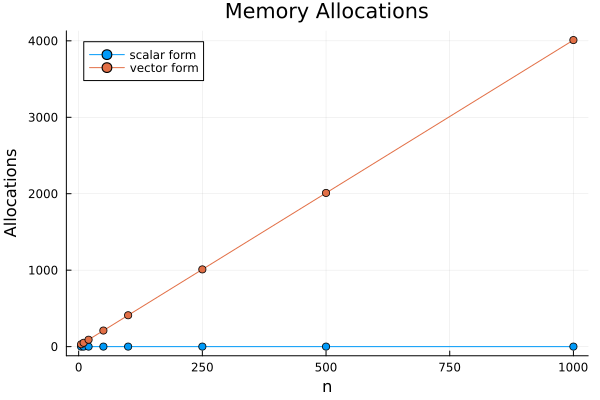
\includegraphics[width=0.48\linewidth]{Plots/memory_allocations.pdf}(a)
 % &    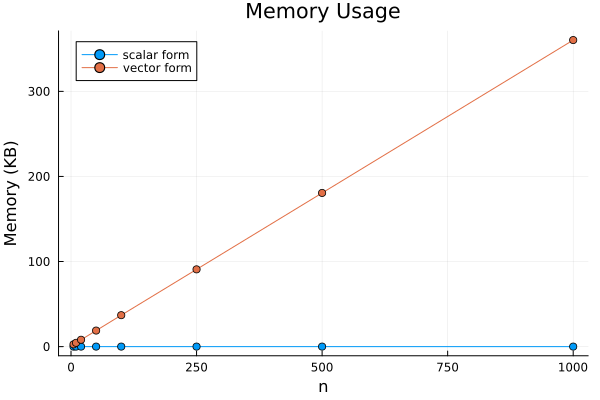
\includegraphics[width=0.48\linewidth]{Plots/memory_usage.pdf}(b) \\  
 %    \multicolumn{2}{c}{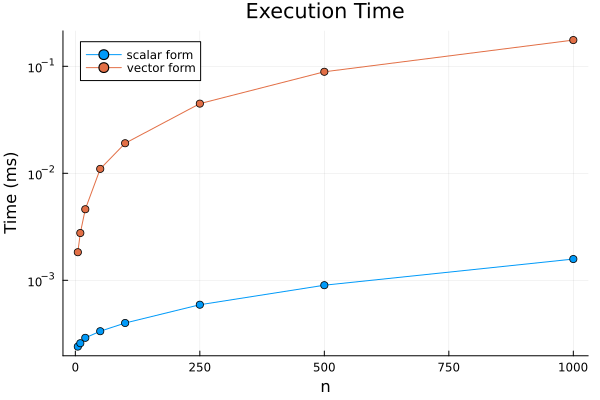
\includegraphics[width=1\linewidth]{Plots/execution_time.pdf}(c)}\\
 %%%%%%%%%%%%%%%%%%%
 %     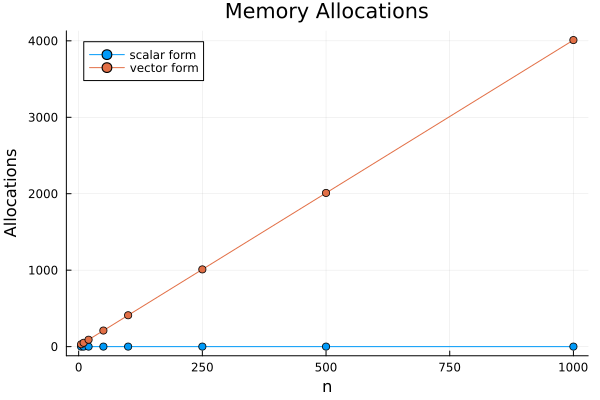
\includegraphics[width=0.48\linewidth]{Plots/memory_allocations.pdf}
 % &    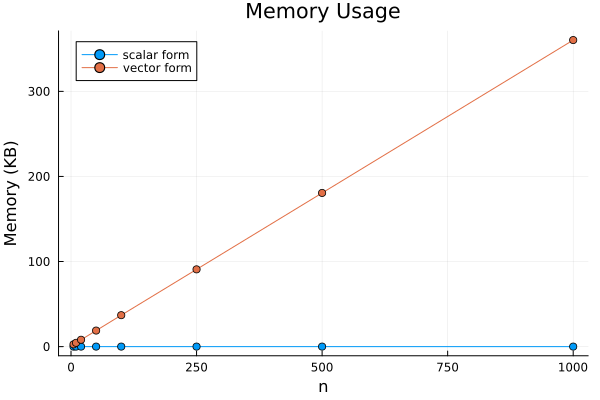
\includegraphics[width=0.48\linewidth]{Plots/memory_usage.pdf} \\ 
 % \footnotesize{(a)} & \footnotesize{(b)} \\
 %    \multicolumn{2}{c}{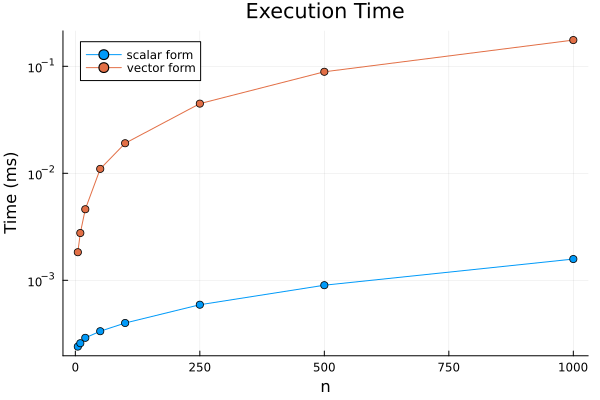
\includegraphics[width=1\linewidth]{Plots/execution_time.pdf}}\\
 %    \multicolumn{2}{c}{\footnotesize{(c)}}\\
 %%%%%%%%%%%%%%%%%%%
      \footnotesize{(a)}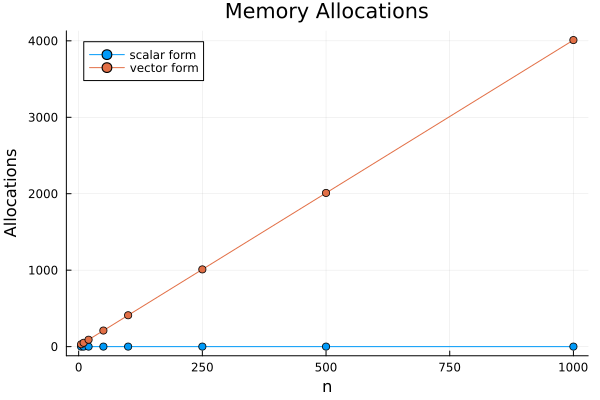
\includegraphics[width=0.48\linewidth]{Plots/memory_allocations.pdf}
 &    \footnotesize{(b)}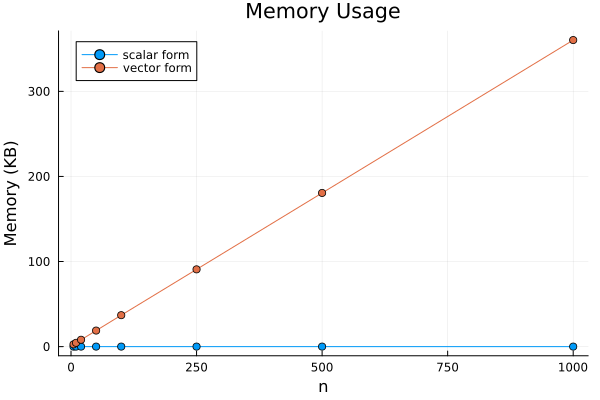
\includegraphics[width=0.48\linewidth]{Plots/memory_usage.pdf} \\[10pt] 
    \multicolumn{2}{c}{\footnotesize{(c)}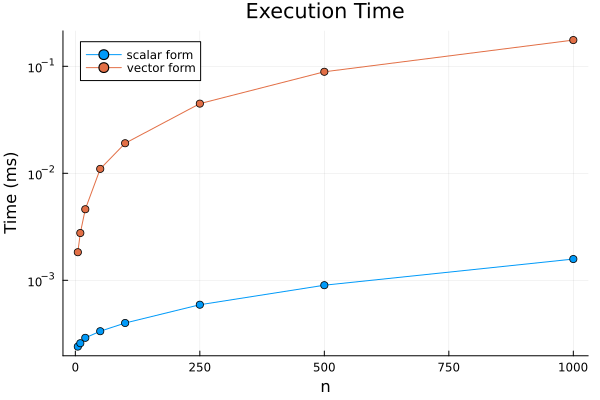
\includegraphics[width=1\linewidth]{Plots/execution_time.pdf}}\\
\end{tabular}
\caption[Performance comparison of cohesions 3 and 4 implementations]{Performance comparison among the three versions of the cohesion 4 function. Similar results stand for cohesion 3. Panels (a) and (b) are constant at zero for both the scalar and static cases.}
% Tests ran through the \mintinline{julia}{BenchmarkTools} package of Julia by randomly generating the spatial coordinates of the various test sizes $n$,
\label{fig: cohesion3 comparison}
\end{figure}

% \begin{figure}[!ht]
% \centering
% % \begin{tabular}{cc}
% %     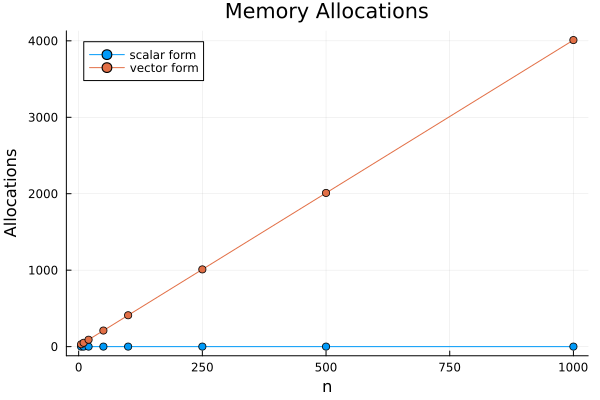
\includegraphics[width=0.5\linewidth]{Plots/memory_allocations.pdf}
% %  &    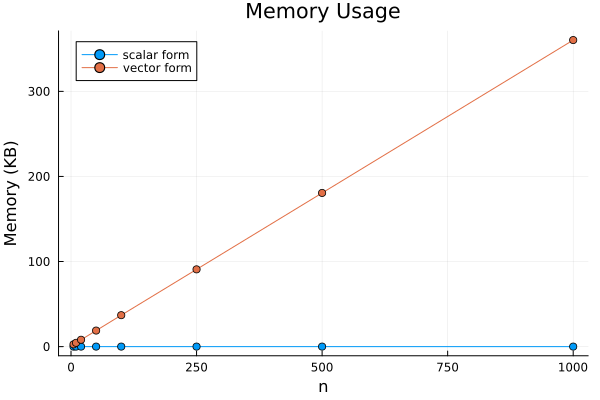
\includegraphics[width=0.5\linewidth]{Plots/memory_usage.pdf} \\  
% %     \multicolumn{2}{c}{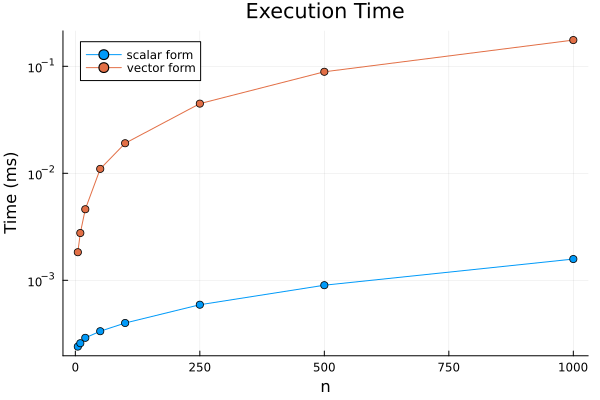
\includegraphics[width=1\linewidth]{Plots/execution_time.pdf} }\\
% % \end{tabular}
%     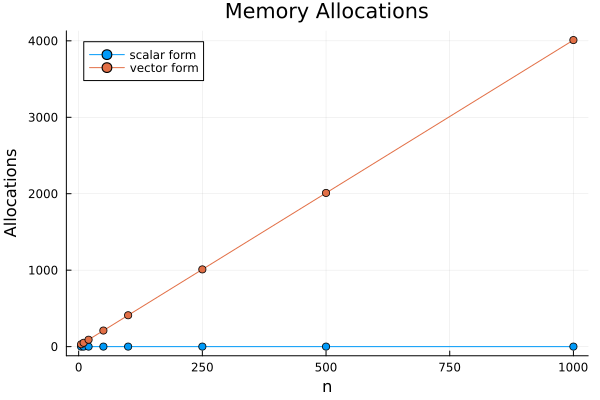
\includegraphics[width=0.5\linewidth]{Plots/memory_allocations.pdf}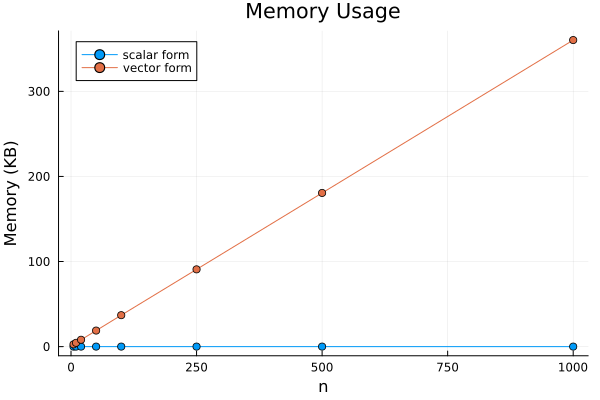
\includegraphics[width=0.5\linewidth]{Plots/memory_usage.pdf} \\  
%     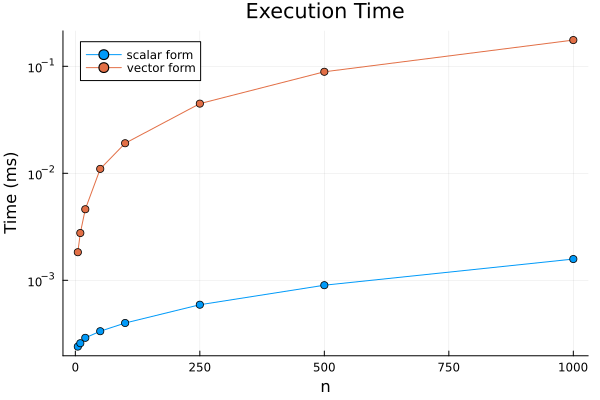
\includegraphics[width=1\linewidth]{Plots/execution_time.pdf}
% \caption[Cohesions 3 and 4 implementation comparison]{Performance comparison between the three versions of the cohesion 4 function. Tests ran through the \mintinline{julia}{BenchmarkTools} package of Julia by randomly generating the spatial coordinates of the various test sizes $n$, with similar results standing for cohesion 3. The memory allocation and usage plots are constant at zero for both the scalar and vector static cases.}
% \label{fig: cohesion3 comparison}
% \end{figure}

This final version employs the \mjline{StaticArrays} package of Julia, which enables more efficient use of vectors and matrices when their sizes are known at compile time. This is suited for the spatial cohesion computations as we consistently work with $2\times 1$ vectors and $2\times 2$ matrices, due to the context of planar spatial coordinates. The benefits of this final implementation include preserving the natural mathematical form of the first solution, thus enhancing code clarity, while also capitalizing on the performance improvements seen in the second solution. In fact, with static structures, the compiler is able to optimize all memory allocations related to vectors and matrices just as it does with simple scalar variables.
% This final version exploits the \mjline{StaticArrays} package of Julia, which allows to use vectors and matrices more efficiently if their size is known at compile time; which is the case of the spatial cohesions computation since working with planar spatial coordinates we will always have $2\times 1$ vectors and $2 \times 2$ matrices. The benefits of this final version are that we maintain the natural mathematical form of the first one, improving the clearness of the code, together with the efficiency of the second one, since now with static structures the compiler is able to optimize all memory allocations as it was doing with the simple scalar variables.

Figure \ref{fig: cohesion3 comparison} provides a performance comparison of the three solutions. Panel \ref{fig: cohesion3 comparison}c proves that the scalar and static versions exhibited similar performance, and both significantly outpaced the initial vector implementation, and both are significantly faster than the initial vector implementation. Additionally, panels \ref{fig: cohesion3 comparison}a and \ref{fig: cohesion3 comparison}b highlight the substantial reduction in memory requirements compared to the first solution. This comparison was conducted by running the three implementations against multiple sets of spatial coordinates with a varying number of units $n$.

% Figure \ref{fig: cohesion3 comparison} shows the comparison of their performances, where we can see how the scalar and static versions indeed perform very similarly to each other, and more quickly with respect to the first version.
Notably, the CDRPM implementation of the corresponding MCMC algorithm was not required to consider these optimizations, since C does not natively support vectors and matrices and was therefore forced to the scalar implementation without much deliberation.
% Noticeably, the C implementation of the model didn't have to worry about all this reasoning, since C can't natively, nor gracefully, work with vectors and matrices and was therefore forced to the scalar implementation. 
% So one point for the old lad.


% \section{Covariates similarities optimized computation}
\subsection{Optimizing covariates similarities}

Another significant challenge that we faced consisted in optimizing the computation of the similarity functions. As the cohesion functions, the similarities would potentially be called millions of times, or even more considering that multiple covariates can be incorporated in the prior and thus introducing an additional loop based on $p$, the number of included covariates. As in the case of the previous analysis, many of the similarity functions did not exhibit a significant need for optimization. However, the fourth function, the auxiliary similarity function, required optimization due to the computational load associated with calculating the sum of the squares of the covariate values, as illustrated in Listing \ref{list: sim4}.
% Another problem has been understanding how to speed up the computation of the similarity functions, since those would also be called possibly millions of times as the cohesion ones or even more, considering that we can incorporate more than one covariate into the clustering process, and this would add an additional loop based on $p$, the number of covariates decided to be included.

% As in the previous case, some of the functions didn't show any special need or room for relevant optimizations. The fourth one instead, the auxiliary similarity function, was essential to be optimized not only because it is one the most common choice among the similarities, but also because it involves a computationally heavy sum of the squares of the covariate values, as we can see in Listing \ref{list: sim4}.

\begin{code}
\caption[Similarity 4 implementation with all optimizing annotations]{Similarity 4 function implementation, with all optimizing annotations. The performance analysis will just focus on that inside loop.}
\label{list: sim4}
\begin{minted}
[breaklines,
baselinestretch=1,
autogobble,
% breaksymbolsepleft=2,
fontsize=\footnotesize,
% linenos
mathescape,
tabsize=4,obeytabs
]{julia}
function similarity4(X_jt::AbstractVector{<:Real}, mu_c::Real, lambda_c::Real, a_c::Real, b_c::Real, lg::Bool)
	n = length(X_jt)
	nm = n/2
	xbar = mean(X_jt)
	aux2 = 0.
	@inbounds @fastmath @simd for i in eachindex(X_jt)
		aux2 += X_jt[i]^2
	end
	aux1 = b_c + 0.5 * (aux2 - (n*xbar + lambda_c*mu_c)^2/(n+lambda_c) + lambda_c*mu_c^2 )
	out = -nm*log2pi + 0.5*log(lambda_c/(lambda_c+n)) + lgamma(a_c+nm) - lgamma(a_c) + a_c*log(b_c) + (-a_c-nm)*log(aux1)
	return lg ? out : exp(out)
end
\end{minted}
\end{code}

The optimization strategy involved annotating the loop with several macros provided by Julia. They were the following:
\begin{itemize}
    \item \mjline{@inbounds} eliminates array bounds checking within expressions. This allows the compiler to bypass these checks, thus saving execution time. This annotation is safe to use as long as we can guarantee that the code will not access elements outside the array bounds; otherwise undefined behaviour may occur. In our case, the loop structure is simple and safe, so this assumption holds true.

    % This allows to skip those checks to save some execution time. This insertion is harmless as long as we are sure that in our code design no out-of-bounds or wrong accesses will occur. Otherwise some undefined behaviour will take place. The above loop is indeed very simple and safe, so this assumption is clearly satisfied. 

    \item \mjline{@fastmath} executes a modified version of the expression that may invoke functions violating strict IEEE semantics\footnote{Institute of Electrical and Electronics Engineers. The IEEE-754 standard specifies floating-point formats, which dictate how real numbers are represented in hardware, along with the expected behaviour of arithmetic operations on them, including precision, rounding, and the handling of special values (e.g., NaN (Not a Number) and infinity).}. For instance, using this macro could result in $(a+b)+c \neq a+(b+c)$, but only in highly pathological cases. Again, this is not an issue for our loop, which computes $\sum X_i^2$, as there is no intrinsic "correct order" for performing this operation.
    % \item \mjline{@fastmath} executes a transformed version of the expression which calls functions that may violate strict IEEE semantics\footnote{Institute of Electrical and Electronics Engineers. The IEEE-754 standard defines floating-point formats, i.e. the ways to represent real numbers in hardware, and the expected behaviour of arithmetic operations on them, including precision, rounding, and handling of special values (e.g. NaN (Not a Number) and infinity).}. For example, its use could make $(a+b)+c \neq a+(b+c)$, but just in very pathological cases. Again, this is not a problem in our function, where we are just computing $\sum X_i^2$, since it does not have an intrinsically "right order" in which it has to be done.

    \item \mjline{@simd} (Single Instruction Multiple Data) allows the compiler to apply further optimizations to the loop. This technique is akin to parallelism; however, rather than distributing the computational load across multiple processors, \mjline{@simd} vectorizes the loop. This means that the CPU can execute the same instruction (summing the square of the $i$-th component into a reduction variable) on multiple data chunks simultaneously using vector registers. As a result, this approach accelerates computation by eliminating the need to process each element of the vector individually.
    % \item \mjline{@simd} (single instruction multiple data) annotate a for loop to allow the compiler to take extra liberties to allow loop re-ordering. This is a sort of parallelism technique, but rather than distributing the computational load on more processors we just \textit{vectorize} the loop, i.e. we enable the CPU to perform that single instruction (summing the square of the $i$-th component to a reduction variable) on multiple data chunks at once, using vector registers, rather than working on each element of the vector individually.
\end{itemize}

\begin{figure}[!ht]
    \centering
    % \includegraphics[width=1\linewidth]{Plots/execution_time_tests_sims.pdf}
    \includegraphics[width=1\linewidth]{Plots/execution_time_tests_sims_pow2.pdf}
    %Their numerical output results are indeed the same for all cases. There are no memory allocation and usage plots since the analysis has been conducted only to evaluate the performances of the inside loop, which has no memory issues.}
    \caption[Performance comparison of similarity 4 annotations]{Performance comparison of the different loop annotations in the similarity 4 implementation.}
    \label{fig: exec time sim}
\end{figure}

As illustrated in Figure \ref{fig: exec time sim}, the observed performance difference primarily arises from the use of \mjline{@simd}, while the other two annotations have minimal impact. Consequently, also to address concerns from pure mathematicians, we opted to remove the \mjline{@fastmath} annotation, retaining only \mjline{@inbounds} and \mjline{@simd}. Memory allocation and usage panels are not reported since the analysis focused solely on evaluating the performance of the inner loop, which does not present any memory-related issues.
% As we can see from Figure \ref{fig: exec time sim}, the actual performance difference basically derives just from the use of \mjline{@simd}, with the other two annotations making not much of a difference. For that reason, and to reassure all pure mathematicians, we decided to remove the \mjline{@fastmath} annotation, leaving just \mjline{@inbounds} and \mjline{@simd}.

Moreover, we observe that experiments employing the \mjline{@simd} annotation tend to run faster when $n$ is a power of two compared to $n$ being its nearest rounded integers, even though this configuration involves processing relatively more data points (for instance, 256 versus 250 or 512 versus 500).
This pattern underscores the effectiveness of the SIMD approach: depending on the architectures, CPUs can support various register sizes (e.g. 64, 128, 256, or 512 bits) and when the total memory occupied by the data points aligns perfectly with these register sizes, i.e. when the number of elements is a power of two, the data can be efficiently loaded into registers without any waste. Conversely, if the data size does not match, there will be "leftover chunks" that still need to be processed, which can introduce some overhead due to the inefficiencies associated with the imperfect fit.
% Interestingly, we also observe that experiments with the \mjline{@simd} annotation execute more quickly when $n$ is a power of two compared to their nearest rounded integers, e.g. 256 versus 250 or 512 versus 500, despite having a relatively larger dataset. 
% This phenomenon demonstrates the effectiveness of the SIMD paradigm: depending on the architecture, CPUs can provide varying register sizes (e.g., 64, 128, 256, or 512 bits). When the total memory occupied by the elements is a multiple of the register size—such as when the number of data values is a power of two—the data can be perfectly subdivided into these registers. Conversely, if this condition is not met, there will be "leftover chunks" that must still be processed. However, this imperfect fit can introduce some overhead due to additional processing requirements.
% We can also notice interestingly how the tests with \mjline{@simd} annotation run quicker in the case of $n$ being a power of two, compared to their closest rounded integers (e.g. 256 against 250 or 512 against 500), despite having relatively some more data. This is a proof of the effectiveness of the SIMD paradigm: according to the different architectures, the CPUs can provide different register sizes (e.g. 64, 128, 256 or 512 bits) and therefore the data subdivision can fit perfectly in them when the total memory occupied by the elements is a multiple of that register size (i.e. the number of data values is a power of two). Otherwise there will be some "leftovers chunks", which will of course be processed, but will also cause, as a consequence of the imperfect fit, a bit of overhead.





\chapter{Analysis of the models}
\label{chap: testing}

% \setlength\epigraphwidth{.65\textwidth}
% \epigraph{\itshape
% I admit that twice two makes four is an excellent thing, but if we are to give everything its due, twice two makes five is sometimes a very charming thing too.
% }{--- F\"{e}dor Dostoevskij, \textit{Notes from the Underground}}
% \setlength\epigraphwidth{.8\textwidth}


In the following analyses, we will make use of the Adjusted Rand Index (ARI) \cite{ari-paper} to compare the partitions generated by the models. The ARI index serves as a correlation metric that quantifies the similarity between two clusterings. Specifically, for two partitions $\rho_1$ and $\rho_2$, the function $\ari(\rho_1,\rho_2)$ produces a value within the range $[-1,1]$ where higher values indicate greater agreement between the partitions. A perfect match $\rho_1=\rho_2$ is represented with the limit case $\ari(\rho_1,\rho_2)=1$.

% In the following analysis we will make use of the Adjusted Random Index (ARI) \cite{ari-paper} to compare the partitions generated by the models. The ARI index is a correlation index to measure similarities between clusterings. More precisely, given two partitions $\rho_1$ and $\rho_2$, the $\ari(\rho_1,\rho_2)$ returns a value between $[-1,1]$ where higher values indicates higher levels of agreement between the partitions, with the limit case of $\ari(\rho_1,\rho_2)=1$ when $\rho_1=\rho_2$. 
% Being a \textit{random} index, it has an expected value and it is equal to zero, which corresponds to the case of comparing two randomly generated partitions. 

We will employ this index to analyse the temporal evolution of the partitions, examining whether $\rho_{t+k}$ correlates with $\rho_{t}$, and to evaluate the level of agreement between the two models, by comparing clusters estimates generated by CDRPM and JDRPM. These clusters estimates will be computed using the \texttt{salso} function, with the binder loss, using the associated \texttt{salso} library \cite{salso} on R.

% We will use this index both to study the time evolution of the clusterings, to see e.g. if $\rho_{t+k}$ is correlated to $\rho_{t}$, that is, how the clusters show the time dependent structure that the models implement, and also to check the level of agreement between the two models, comparing the clusters produced by CDRPM and JDRPM.

All analyses of this Chapter were conducted on a laptop equipped with 8 GB of RAM and a 1.80 GHz CPU base clock speed. The software used was R \cite{R-cite}, interfaced with Julia through the \texttt{JuliaConnectoR} library \cite{juliaconnectoR}.
% This library handled all the communication between R and Julia, where the JDRPM's MCMC algorithm is implemented.
The CDRPM implementation was also accessible from R via a dedicated package, \texttt{drpm}, developed by \cite{1-drpm}, which similarly employs a wrapper to invoke the C code where the MCMC algorithm is implemented.

% All the following runs have been performed on my laptop, which for performance references has 8 GB of RAM and 1.80 GHz CPU base clock speed, on the software R \cite{R-cite} and through the \tt{JuliaConnectoR} library \cite{juliaconnectoR}, which allowed the interface between R and Julia where JDRPM is implemented. The CDPRM is also accessible from R through a dedicated package \tt{drpm}, which also uses a similar wrapper to call native C code.


\section{Comparing the two algorithms}
\label{Assessing the equivalence of the models}

Our model, along with its corresponding MCMC algorithm, represents a generalization of the original DRPM and its associated algorithm. The improvements, as outlined in previous chapters, include the ability to incorporate covariates into both the prior and likelihood levels of the Bayesian model, the possibility of allowing for missing data in the response variable, and the guarantee of greater computational efficiency. In this regard, our updates serve as extensions to the original model; therefore, when tested under identical datasets, hyperparameters, and MCMC configurations, both models are expected to perform similarly and produce comparable clusters estimates.

% Our model, and the corresponding Julia code, is an improvement of the original DRPM with his relative C implementation. These improvements, as described in the previous chapters, refer to the possibility of adding covariates in the Bayesian model, in the prior and in the likelihood, the possibility of allowing for missing data in the response, and the computational efficiency. In this sense, our updates are just add-ons to the original model, and therefore at a common testing level, i.e. under equivalent hyperparameters and MCMC setup, they should perform similarly by agreeing in the clusters that they produce on a given dataset.

To evaluate the numerical performance of both algorithms, we will analyse posterior samples and clusters estimates in two scenarios: first using a synthetic dataset that includes only the response variable, and secondly employing a real-world spatio-temporal dataset. The latter also provides covariates; however, their effects will be extensively examined in the dedicated Section \ref{Effects of the covariates}.\noclub

% To assess this ideally equivalent behaviour we ran two tests: the first one with only the target values, using synthetic data, while the second including spatial information, using a real spatio-temporal dataset.
% For the sake of clarity, also in these sections we will refer to CDRPM for the original model and implementation from \cite{1-drpm}, while to JDRPM for the updated version derived from this thesis work.

\subsection{On a synthetic dataset}
\label{Target variable only}

For the initial comparison we generated a dataset consisting of $n=10$ units and $T=12$ time instants. The data generating function was the same employed in \cite{1-drpm} for their analyses, and it allows for the creation of data points with temporal dependence. %which could be adjusted through specific parameters. 
Regarding the MCMC setup, both algorithms were executed deriving 2000 iterates from a total of 50000 iterations, by discarding the first 40000 as burnin and then thinning by 5. Both models were fitted using a time specific $\alpha$ and using their full formulations, i.e. including and updating also the optional autoregression parameters $\eta_{1i}$ and $\phi_1$.


\begin{table}[!htb]
    % \caption[Accuracy metrics of CDRPM and JDRPM fits, target values only]{Summary of the comparison between the two fits on target values only. The MSE columns refer to the accuracy between the fitted values generated by the models (estimated by taking the mean and the median of the returned 1000 iterates) and the true values of the target variable. Higher LPML and lower WAIC indicate a better fit.}
    \caption[Comparison of CDRPM and JDRPM, simulated data scenario]{Comparison between CDRPM and JDRPM fits and their associated algorithms, in the simulated data scenario.}
    \centering
    % \begin{tabular}{cccccc}
    \begin{tabular}{cccc}
    \toprule
       % & MSE mean &  MSE median & LPML & WAIC & exec. time  \\
       % \midrule
       %  CDRPM &  1.6731  & 1.5861  & -249.61 & 469.69 & 4.8s\\
       %  JDRPM & \textbf{1.2628}  & \textbf{1.2181}  & \textbf{-227.83} &  \textbf{415.03}  &  \textbf{2.5s} \\
       %  \bottomrule
          & MSE mean &  MSE median & execution time  \\
       \midrule
        CDRPM &   1.6221  &  1.5823  & 19s\\
        JDRPM & \textbf{1.2634}  & \textbf{1.2034}  &   \textbf{13s} \\
        \bottomrule
    \end{tabular}
    \label{tab: fits metrics no space}
\end{table}

\begin{figure}[!htb]
    \centering
    \includegraphics[width=1\linewidth]{Testing/Assessing correctness/no space/ari.pdf}
    \caption[Lagged ARI values of CDRPM and JDRPM, simulated data scenario]{Lagged ARI values of CDRPM and JDRPM fits, in the simulated data scenario.}
    \label{fig:ari no space}
\end{figure}

During this first experiment, the clusters were defined solely by the target values from $Y_{it}$, and both models achieved satisfactory results. Fitted values are presented in Figure \ref{fig: fitted and target values no space} alongside the original data. From Table \ref{tab: fits metrics no space} we can see how JDRPM exhibited greater accuracy, as proven by the lower mean squared error (MSE), and a faster execution time. In the table, the MSEs were computed by comparing the fitted values generated by the models, estimated through the mean and the median of the 2000 iterations, with the true values of the target variable. We do not report fitting metrics for WAIC and LPML since, in this first analysis, both models were conceptually equivalent and tested under identical conditions. Consequently, any observed differences in these metrics would be likely attributable to chance.
% change or random variations

% At this testing stage there were just the target values from $Y_{it}$ to dictate the clusters definition, and both models managed to provide good fits, as we can read from Table \ref{tab: fits metrics no space}. In the table, the MSE columns refer to the accuracy between the fitted values generated by the models (estimated by taking the mean and the median of the returned 2000 iterates) and the true values of the target variable. We can see how JDRPM obtained a faster execution time, which is however not really relevant in this small-sized fit. Regarding the fitted values, displayed in Figure \ref{fig: fitted and target values no space} together with the original data, they turned out to be also more precise than the one generated by CDRPM, having lower mean squared errors. We do not report the fitting metrics of WAIC and LPML since the models were conceptually equivalent and tested under the same hyperparameters and MCMC iteration setup. Therefore, any observed difference in these metrics could be likely attributed to chance.

\begin{figure}[!htb]
    \centering
    \includegraphics[width=1\linewidth]{Testing/Assessing correctness/no space/partizioni_nums.pdf}
    \caption[Clusters estimates of CDRPM and JDRPM, simulated data scenario]{Clusters estimates produced by CDRPM and JDRPM fits, in the simulated data scenario. Time instants are annotated on the $x$ axis, units are indicated vertically by their number, and colors represent the cluster label.}
    \label{fig:partizioni no space}
\end{figure}
\begin{figure}[!htb]
    \centering
    \includegraphics[width=1\linewidth]{Testing/Assessing correctness/no space/clusters_C.pdf}
    \includegraphics[width=1\linewidth]{Testing/Assessing correctness/no space/clusters_J.pdf}
    \caption[Visual representation of the clusters estimates of CDRPM and JDRPM, simulated data scenario]{Visual representation of the clusters estimates produced by CDRPM and JDRPM fits, in the simulated data scenario. Cluster labels are represented as colored dots overlaid to the trend of the target variable.}
    \label{fig:clusters no space}
\end{figure}



% The resulting partitions, estimated using the \texttt{salso} function from the corresponding R library \cite{salso}, were remarkably similar. Their temporal trend, depicted in Figure \ref{fig:ari no space}, shows how both models accurately captured the temporal trend of the response variable. Figures \ref{fig:partizioni no space} and \ref{fig:clusters no space} illustrate the clusters estimates, from which we can see how only two minor differences occurred, that we will now address.

% The resulting clusters, estimated using the \mjline{salso} function from the corresponding R library \cite{salso}, were indeed very similar. Figure \ref{fig:ari no space} shows how they manifest the same temporal trend, while Figure \ref{fig:partizioni no space} highlights how the clusters produced are effectively the same except for some small differences that we now discuss.
% Although this was a simple test, there is still room for relevant comments. 


As illustrated in Figure \ref{fig:ari no space}, both models effectively captured the same temporal trend of the clusters. Indeed, the estimated partitions were remarkably similar, as proven by Figure \ref{fig:partizioni no space}, except for two minor differences which we will now discuss. 

A closer examination of the clusters presented in Figure \ref{fig:clusters no space} reveals interesting distinctions at times $t=1$ and $t=9$. At $t=1$, JDRPM classified unit 7 as a singleton within the green cluster, whereas CDRPM assigned it to the black cluster. Both classifications are reasonable: the data point is indeed closer to the black cluster, but it later aligns more distinctly to the red cluster, suggesting the classification given by JDRPM as a detection of its initial anomalous behaviour. At $t=10$, both models successfully identified a small, temporary third cluster resulting from the transition of units 9 and 10. The JDRPM interprets this transition as a label swap: between times $t=9$ and $t=11$, unit 9 shifts from the red cluster to the black cluster, while unit 10 from the black cluster to red cluster. In contrast, at $t=9$ CDRPM assigns both units to the red cluster, potentially reflecting a misclassification considering the temporal trend of unit 10 which, until $t=10$, exhibited a closer alignment with the black cluster.

% By visually inspecting the clusters from Figure \ref{fig:clusters no space}, we can see how at $t=1$ the JDRPM assigned posed unit 7 into a singleton, the green cluster, while CDRPM assigned it into the black label. Both choices seem reasonable: that data point is closer to the black pack, however in the following time instants would be clearly part of the red cluster, therefore we could interpret that closeness as an anomalous behaviour which would require a singleton. At time $t=10$, both models are able to identify a small third cluster, created from the transition of units 9 and 10 to opposite clusters between times $t=9$ and $t=11$. That is, unit 10 transitions among black, green, red; while unit 9 among red, green, black. While JDRPM manages to capture this change, CDRPM at $t=9$ assigns unit 10 still to the red cluster in a possibly improper way.


\begin{figure}[!p]
    \centering
    \includegraphics[width=0.97\linewidth]{Testing//Assessing correctness//no space/test_1_generated_data.pdf}
    \includegraphics[width=0.97\linewidth]{Testing//Assessing correctness//no space/C_mean_prediction.pdf}
    \includegraphics[width=0.97\linewidth]{Testing//Assessing correctness//no space/J_mean_prediction.pdf}
    \caption[Fitted values of CDRPM and JDRPM, simulated data scenario]{Fitted values of CDRPM (middle) and JDRPM (bottom) fits, in the simulated data scenario, alongside the generated target values (top).}
    \label{fig: fitted and target values no space}
\end{figure}


\subsection{On spatio-temporal data}
\label{On spatio-temporal data}

In this section we examine a real-world application by fitting CDRPM's and JDRPM's MCMC algorithms on a spatio-temporal dataset. Specifically, we used the AgrImOnIA dataset \cite{agrimonia} which encompasses measurements of air pollutants, together with many other environmental variables, in the Lombardy region of Italy from 2016 to 2021. 

% We now consider a more realistic scenario in which we fit the models using a spatio-temporal dataset. In particular, we used the AgrImOnIA \cite{agrimonia} dataset which stores measurements about air pollutants, together with many other environmental variables, in the Lombardy region from 2016 to 2021. For the following testing fits, we employed a summary dataset composed by weekly averages of the data from year 2018. 

\begin{figure}[!ht]
    \centering
    % \includegraphics[width=1\linewidth]{Testing/Covariates/corollary images/WE_tot_precipitationcentered wrt global mean.pdf}
    % \includegraphics[width=1\linewidth]{Testing/Covariates/corollary images/WE_tot_precipitationcentered wrt time-wise mean.pdf}
    \includegraphics[width=1\linewidth]{Testing/Covariates/corollary images/AQ_pm10centered wrt global mean.pdf}
    \includegraphics[width=1\linewidth]{Testing/Covariates/corollary images/AQ_pm10centered wrt time-wise mean.pdf}
    \caption[Comparison of the two mean centering methods]{Values of the target variable \tt{AQ\_pm10} adjusted using the global mean (top) and the time-wise mean (bottom). Coloring is based on the ranking of $\pmten$ values of the units according to their median, from highest (red) to lowest (blue).}
    \label{fig:different means conceptions PM10}
\end{figure}
% This second choice helps to adjust the values range while keeping, or even highlighting, the clustering structural information. 


For our subsequent analyses, we employed a dataset comprising weekly averages from the year 2018. The target variable chosen for these studies was $\pmten$, which represents the concentration of particulate matter with a diameter of less than \SI{10}{\micro\metre}. This variable underwent log-transformation, to recover a normal distribution, and was centered with respect to time-wise means. More precisely, each observation $Y_{it}$ was adjusted by subtracting the mean $\bar{Y}_t$ of all observations at that time instant $t$. This approach, consistent with the methodology employed by \cite{1-drpm} during their analyses, helps to emphasize variations within each time point rather than across the entire dataset. This approach is particularly beneficial for understanding how individual units deviate from their typical behaviour at specific times, thereby highlighting temporal trends and anomalies. Moreover, this method effectively mitigates any temporal bias that may arise from periods in which all target values are disproportionately high or low due to external anomalous factors. In contrast, the traditional approach of centering the data around their global mean $\bar{Y}$ would primarily facilitate the detection of overall trends, without providing an elaborate examination of each time step. For instance, preliminary analyses using global centering revealed only three clusters across all time points. While this result is indeed valid in light of the trend illustrated in Figure \ref{fig:different means conceptions PM10}, our alternative approach produced multiple clusters, thereby enhancing the specialization of the clusters together with their interpretability.

% For our subsequent analyses, we employed a dataset consisting of weekly averages of the year 2018. The chosen target variable was $\pmten$ whose values had been log-transformed, to recover a normal distribution, and centered with respect to time-wise means. More precisely, each unit $Y_{it}$ was corrected by subtracting the mean $\bar{Y}_t$ of all the observations of that time instant. This procedure, which was the same employed by the authors of the original DRPM during their spatial tests, helps to emphasize the variations within each time point rather than across the entire dataset. This can be particularly useful to understand how units deviate from their typical behaviour at specific times, potentially highlighting temporal trends and anomalies. 
% This method also removes any temporal bias, e.g. time instants in which all target values were particularly high or low for any particular reason. In contrast, the more traditional choice of centering with respect to the global mean $\bar{Y}$ of the dataset would be useful to just detect global trends, without inspecting deeply into each step. From some test fits performed on the target values with the classical global centering indeed only three clusters appeared, for all time instants. This is of course correct, in some sense, since it's reasonable according to the trend displayed in the top image of Figure \ref{fig:different means conceptions PM10}. However, as we will see shortly, the other version was able to produce several clusters, or at least different partitions at different time instants, improving the specializations of the clusters and the interpretability of the obtained results.

To perform the fit, we used all the available stations in the dataset, amounting to $n=105$, but restricted the time horizon to $T=12$, corresponding to a three-month monitoring period. This limitation was implemented solely to reduce the computational time required to conduct the analyses. As in the previous section, both CDRPM's and JDRPM's MCMC algorithms were fitted with a time-specific parameter $\alpha$ and using their complete model formulations including the optional parameters $\eta_{1i}$ and $\phi_1$. Regarding the spatial cohesion, we selected $C_3$, the auxiliary similarity function. To ensure convergence, we inspected the trace plots of both model and, in the case of JDRPM, we checked numerical diagnostics as the Effective Sample Size (ESS) and $\hat R$. In fact, the JDRPM's implementation is able to provide such statistical assessments directly from the Julia fitting function. Regarding the MCMC setup, we derived 4000 iterates from 110000 total iterations, by discarding the first 90000 as burnin and then thinning by 5.

% We took all the $n=105$ stations available in the dataset but we limited the time horizon to $T=12$, which corresponds to a three-month monitoring period, just to reduce the time needed to perform all tests. We ran both CDRPM and JDRPM models using the same complete modelling setup, as in Section \ref{Target variable only}, and using a time specific $\alpha$. Convergence was ensured visually by inspecting trace plots and, for the JDRPM model, by numerical diagnostics such as ESS and $\hat R$, which instead the CDRPM model is not able to provide directly from the fit. We collected 4000 iterates, from 110000 total iterates with a burnin of 90000 and thinning by 5. 

\begin{table}[!ht]
    \caption[Comparison of CDRPM and JDRPM, real-world scenario]{Comparison between CDRPM and JDRPM fits and their associated algorithms, in the real-world scenario.}
    % Higher LPML and lower WAIC indicate a better fit.}
    \centering
    \begin{tabular}{cccc}
    \toprule
          % & \multicolumn{2}{c}{MSE using} & \multicolumn{2}{c}{Fit metrics} & \\
           % \cmidrule(lr){2-3}
           % \cmidrule(lr){4-5}
       % & MSE mean &  MSE median & LPML & WAIC & exec. time  \\
       % \midrule
       %  CDRPM &   0.0142   & 0.0149   & \textbf{ 694.81} & -1768.42 & 1h38m\\
       %  JDRPM & \textbf{0.0131}  & \textbf{0.0138}   & 624.91 & \textbf{-1898.05}  &  \textbf{48m}\\
       %  \bottomrule
              & MSE mean &  MSE median & execution time  \\
       \midrule
        CDRPM &   0.0142   & 0.0149  & 1h38m\\
        JDRPM & \textbf{0.0131}  & \textbf{0.0138}    &  \textbf{48m}\\
        \bottomrule
    \end{tabular}
    \label{tab: fits metrics space}
\end{table}


\begin{figure}[!ht]
    \centering
    \includegraphics[width=1\linewidth]{Testing/Assessing correctness/space/ari.pdf}
    \caption[Lagged ARI values of CDRPM and JDRPM, real-world scenario]{Lagged ARI values of CDRPM and JDRPM fits, in the real-world scenario.}
    \label{fig:ari space}
\end{figure}


\begin{figure}[!p]
    \centering
    \includegraphics[width=0.97\linewidth]{Testing//Assessing correctness//space/test_2_spatial_data.pdf}
    \includegraphics[width=0.97\linewidth]{Testing//Assessing correctness//space/C_mean_prediction.pdf}
    \includegraphics[width=0.97\linewidth]{Testing//Assessing correctness//space/J_mean_prediction.pdf}
    \caption[Fitted values of CDRPM and JDRPM, real-world scenario]{Fitted values of CDRPM (middle) and JDRPM (bottom) fits, in the real-world scenario, alongside the generated target values (top).}
    % \caption[Target and fitted values of JDRPM and CDRPM fits, target plus space values]{Target $Y_{it}$ values (top), together with their fitted values estimate through the mean of the 4000 iterates generated by model CDRPM (middle) and JDRPM (bottom).}
    \label{fig: fitted and target values space}
\end{figure}

Table \ref{tab: fits metrics space} demonstrates that both models achieved remarkable accuracy in their fitted values, with JDRPM leading over CDRPM in terms of MSEs. As previously mentioned, we have chosen not to report the fitting metrics for WAIC and LPML due to the theoretical equivalence of the evaluated models and their corresponding MCMC setup. While execution times are included, they may not fully reflect the actual performance, as when performing the fits I was concurrently engaged in writing this thesis, which limited my laptop's computational resources for the fitting process. Nonetheless, more precise assessment of performance timings will be presented in Section \ref{chap: Scaling performances}.
% Table \ref{tab: fits metrics space} shows how both model managed to be accurate in terms of the fitted values, with JDRPM again performing better in terms of MSEs. As in the previous section, we do not report the fitting metrics of WAIC and LPML because of the theoretical equivalence of the models. Execution times are also reported, but they are somewhat inaccurate since during the fitting I was busy in writing this thesis, meaning that not all the computational resources of my laptop were devoted to the fitting task. In any case, more precise performance evaluations on the timings will be conducted in Section \ref{chap: Scaling performances}.

Figure \ref{fig:ari space} reveals a similar temporal trend, further validating the correct implementation of JDRPM's MCMC algorithm. In terms of clusters similarity, a partition plot as in Figure \ref{fig:partizioni no space} would appear more congested due to the increased number of units. To effectively convey this information, we computed the adjusted Rand index $\ari(\rho_{\text{JDRPM}}(t),\rho_{\text{CDRPM}}(t))$ for all time points $t=1,\ldots,12$. The results yielded a mean of 0.80 and a median of 0.86, denoting a strong agreement between the clusters estimates generated by the two models.
% From Figure \ref{fig:ari space} we can see how the temporal trend was very similar, confirming again the correctness of the JDRPM implementation. Regarding the similarity of the produced clusters, the partition plot as the one of Figure \ref{fig:partizioni no space} would now be more crowded due to the high number of units. For this reason, in order to still convey that information, we computed $\ari(\rho_{\text{JDRPM}}(t),\rho_{\text{CDRPM}}(t))$ for all time instants $t=1,\ldots,12$, and we obtained a mean of 0.80 and a median of 0.86, denoting high levels of agreement in the clusters produced.

% \begin{figure}[!p]
%     \centering
%     \includegraphics[width=1\linewidth]{Testing/Assessing correctness/simple maps/fitCDRPM target + space_simple_map.pdf}
%     \includegraphics[width=1\linewidth]{Testing/Assessing correctness/simple maps/fitJDRPM target + space_simple_map.pdf}
%     \caption[Visual representation of the clusters estimates of CDRPM and JDRPM, real-world scenario]{Visual representation of the clusters estimates produced by CDRPM and JDRPM fits, in the real-world scenario.}
%     % \caption[Clusters generated by CDRPM and JDRPM fits, target plus space values]{Clusters generated by the CDRPM and JDRPM fits with target plus space values.}
%     \label{fig:clusters space basic simple}
% \end{figure}

% Figure \ref{fig:clusters space basic simple} offers a visual representation of the clusters, which will be discussed in greater detail in Section \ref{Covariates in the clustering}. This section will also include an analysis of the fits that incorporate covariates into the clustering process.
A visual representation of the clusters estimates generated by the two models is provided in Figures \ref{fig:clusters visualized CDRPM space} and \ref{fig:clusters visualized JDRPM space}. Nevertheless, a more comprehensive analysis and discussion of the generated clusters will take place in Section \ref{Covariates in the clustering}, where we will also examine fits which include covariates in the prior and likelihood levels.
% A visual representation of the clusters is provided in Figure \ref{fig:clusters space basic simple}, but will be further detailed and commented in Section \ref{Covariates in the clustering} together with the fits including covariates in the clustering.



% \begin{figure}[!ht]
%     \centering
%     \includegraphics[width=1\linewidth]{Testing/Assessing correctness/space/clusters_C.pdf}
%     \includegraphics[width=1\linewidth]{Testing/Assessing correctness/space/clusters_J.pdf}
%     \caption[Visual representation of the clusters of the JDRPM and CDRPM fits with target plus space values]
% {Visual representation of the clusters produced by the models, on the fit with target plus space data, with units' labels represented as colored dots overlaid to the trend of the target variable.}
%     \label{fig:clusters space}
% \end{figure}



% \begin{figure}[!p]
%     \centering
%     \includegraphics[width=1\linewidth]{Testing/Covariates/corollary images/LA_hvi.pdf}
%     \includegraphics[width=1\linewidth]{Testing/Covariates/corollary images/LA_hvi.pdf}
%     \includegraphics[width=1\linewidth]{Testing/Covariates/corollary images/LA_hvi.pdf}
%     \caption{Enter Caption}
%     \label{fig:enter-label}
% \end{figure}



% \section{Behaviour in presence of missing values}
\section{Performance with missing values}
\label{Performance with missing values}

In this section, we replicate the analyses and evaluations from Section \ref{Assessing the equivalence of the models}, this time focusing on scenarios involving missing values. Our objective is to investigate how the JDRPM performs in the absence of complete datasets and to determine whether it maintains effective performances under such conditions.

Given the extent of missing values in the AgrImOnIA dataset \cite{agrimonia}, which was used for the spatio-temporal analysis, we opted to set 10\% of the values as missing (NAs). To implement this, we randomly selected $nT/10$ indexes from the sets $[1,\ldots,n]$ and $[1,\ldots,T]$ to identify all the pairs $(i,t)$ that would be designated as missing in the target variable $Y_{it}$. The ability to handle missing data is an enhancement introduced by the JDRPM; therefore these studies cannot be repeated with the original CDRPM, which does not accept incomplete datasets.

% We now repeat the analyses and evaluations of the previous section in both scenarios but, this time, with missing values, to see how the JDRPM model reacts to the absence of a full dataset and check if it can still perform well. Based on the amount of missing values in the AgrImOnIA dataset \cite{agrimonia}, used for the spatio-temporal tests, we chose to set at 10\% the amount of values that would be replaced by NAs. To perform such replacements, we randomly drew $nT/10$ indexes from the sets $[1,\ldots,n]$ and $[1,\ldots,T]$ to get all the pairs $(i,t)$ which would become missing values in the target variable $Y_{it}$. The dealing of NAs was an upgrade brought by the JDRPM model, so we cannot perform these tests with the original CDRPM model since it cannot handle missing data. 

All the following fits were conducted under the same conditions of their full-dataset counterpart, i.e. using the same models formulation, parameters, and MCMC setup.

\begin{figure}[!ht]
    \centering
    % \includegraphics[width=1\linewidth]{Testing/NA data/no space NA/test_1_generated_data.pdf}
    \includegraphics[width=1\linewidth]{Testing/NA data/no space NA/J_mean_prediction.pdf}
    % \caption{Generated target values (top), together with their fitted values estimate through the mean of the 1000 iterates generated by model JDRPM (bottom). Special point markers are devoted to the data points corresponding to missing values, to highlight the gaps between the fit on the full dataset and the fit on the NA dataset.}
    \caption[Fitted values of JDRPM, simulated data scenario, dataset with missing values]{Fitted values of JDRPM fit, in the simulated data scenario, with missing values in the target variable. Special square markers are devoted to the data points which were missing, highlighting the gaps between the fitted values on the full dataset (green) and the fitted values on the dataset with missing values (red).}
    \label{fig: target values estimates no space NA}
\end{figure}

\subsection{No spatial information}
\label{No spatial information}

The JDRPM demonstrated remarkable performance even in the presence of missing values. As shown in Table \ref{tab: fits metrics no space julias na full}, the model's performance is understandably lower compared to the full dataset scenario; however, it clearly remains satisfactory. The MSE has naturally increased due to the absence of some data points, which produced less accurate fitted values for the corresponding missing entries. Nevertheless, the fitted values, illustrated in Figure \ref{fig: target values estimates no space NA}, remain closely aligned with the ones derived from the full dataset analysis.

% The JDRPM seems to exhibit good performance also with missing values. From Table \ref{tab: fits metrics no space julias na full} we can see how the performances are naturally worse than the fit in the full case, but are still good. The MSE is inevitably higher since the model did not see all the data points, resulting in less precise fitted values for the corresponding missing spots in the dataset. Nonetheless, the fitted values, represented in Figure \ref{fig: target values estimates no space NA}, are still close the one obtained with the fit on full dataset. 

\begin{table}[!ht]
    \caption[Comparison of JDRPM, simulated data scenario, dataset with missing values]{Comparison of JDRPM fits, in the simulated data scenario, on a complete dataset and on a dataset with missing values.}
    \centering
    \begin{tabular}{cccccc}
    \toprule
          % & \multicolumn{2}{c}{MSE using} & \multicolumn{2}{c}{Fit metrics} & \\
           % \cmidrule(lr){2-3}
           % \cmidrule(lr){4-5}
            & MSE mean &  MSE median & LPML & WAIC & exec. time  \\
           % & mean &  median & LPML & WAIC & execution time  \\
           \midrule
        NA data &   1.4721   & 1.2101 & -236.93 & 401.44 & 13s\\
        full data& 1.2634 & 1.2034  & -223.36 & 393.97  &  13s \\
        \bottomrule
    \end{tabular}
    \label{tab: fits metrics no space julias na full}
\end{table}


\begin{figure}[!ht]
    \centering
    \includegraphics[width=1\linewidth]{Testing/NA data/no space NA/partizioni_nums.pdf}
    \caption[Clusters estimates of JDRPM, simulated data scenario, dataset with missing values]{Clusters estimates produced by JDRPM fits, in the simulated data scenario, on a dataset with missing values. Time instants are annotated on the $x$ axis, units are indicated vertically by their number, and colors represent the cluster label.}
    \label{fig: partizioni no space NA}
\end{figure}

\begin{figure}[!ht]
    \centering
    \includegraphics[width=1\linewidth]{Testing/NA data/no space NA/ari.pdf}
    \caption[Lagged ARI values of JDRPM, simulated data scenario, dataset with missing values]{Lagged ARI values of JDRPM fits, in the simulated data scenario, on a dataset with missing values.}
    \label{fig:ari no space NA}
\end{figure}

\begin{figure}[!ht]
    \centering
    \includegraphics[width=1\linewidth]{Testing/NA data/no space NA/clusters_J.pdf}
    \caption[Visual representation of the clusters estimates of JDRPM, simulated data scenario, dataset with missing values]{Visual representation of the clusters estimates produced by JDRPM fit, in the simulated data scenario, on a dataset with missing values. Cluster labels are represented as colored dots overlaid to the trend of the target variable, with special point markers devoted to data points corresponding to missing values.}
    \label{fig:clusters no space NA}
\end{figure}

\begin{figure}[!ht]
    \centering
    % \includegraphics[width=1\linewidth]{Testing/NA data/no space NA/target_only_NA_CIs.pdf}
    \includegraphics[width=1\linewidth]{Testing/NA data/no space NA/target_only_NA_CIs_SORTED.pdf}
    \caption[Credible intervals of JDRPM, simulated data scenario, dataset with missing values]{Credible intervals, computed with the highest posterior density (HPD) method at a 95\% confidence, for the fitted values of the missing units in the JDRPM fit, in the simulated data scenario, on a dataset with missing values. In gray are reported the indexes of units $i$ and time instants $t$ which where missing, while green dots refer to the true values of the missing data.}
    \label{fig: CIs target only}
\end{figure}

From Figure \ref{fig:ari no space NA}, we observe a nearly identical temporal trend to the trend of the full dataset analysis, indicating how JDRPM effectively captured a robust temporal dependency structure even when some data points were missing. Additionally, the clusters generated, as shown in Figure \ref{fig:clusters no space NA}, appeared remarkably similar. The only notable difference occurred around time $t=10$, where the model now failed to identify the green cluster that characterized the final transition phase of units 9 and 10. This discrepancy may be attributed to the NA assignment of unit 9 at time 10, which likely removed critical information necessary for identifying that specific third cluster.
% From Figures \ref{fig:ari no space NA} we can see how we get almost the same temporal trend which we saw in the case without missing data, meaning that the JDRPM is able to recover a good temporal dependency structure even if some data are missing. Also the generated clusters, represented in Figure \ref{fig:clusters no space NA}, appeared to be really similar. The only relevant different occurred at time $t=10$, where now the model was not able to identify the green cluster which characterized the final transition phase of units 9 and 10. This is possibly due to the fact that the random creation of the NA data set unit 9 at time 10 to be missing, therefore removing important information for the retrieving of that special third cluster.  

Finally, Figure \ref{fig: CIs target only} presents the 95\% credible intervals for the fitted values corresponding to the missing data points. Except for one case, the true value always fell within the credible interval, demonstrating the accuracy of JDRPM in providing reliable estimates of the target values, even in situations where no additional information was available from either space or covariates.
% Finally, Figure \ref{fig: CIs target only} shows the 95\% credible intervals for the fitted values corresponding to the missing data points. We can see how in almost all cases, except for one, the true value lies inside the credible interval, denoting the accuracy of JDPRM in retrieving good estimates of the target values, even in this case where no additional information was available either through space or covariates.


\subsection{With spatial information}
\label{With spatial information}

The JDRPM demonstrated robust performance also in real-world scenario involving a dataset with missing values. Table \ref{tab: fits metrics space julias na full} indicates a slight reduction in accuracy, which is expected due to the presence of missing data; however, the decline is not substantial. The fitted values are displayed in Figure \ref{fig: target values estimates space NA}, revealing how the estimation of the missing data becomes more challenging for the points that lie farther away from the main trajectory of the distribution. It is worth noting that the reported execution times may not fully reflect reality, as previously mentioned, due to my laptop’s resources not being entirely devoted to the fitting process. In fact, the JDRPM fit with missing data ran faster than the JDRPM fit with complete data, which raises some eyebrows since we should expect additional computational demands when dealing with missing $Y_{it}$ values, due to their sampling step in the MCMC algorithm. Again, for more accurate performance assessments we refer to Section \ref{chap: Scaling performances}.

\begin{table}[!ht]
    \caption[Comparison of JDRPM, real-world scenario, dataset with missing values]{Comparison of JDRPM fits, in the real-world scenario, on a complete dataset and on a dataset with missing values.}
    \centering
    \begin{tabular}{cccccc}
    \toprule
          % & \multicolumn{2}{c}{MSE using} & \multicolumn{2}{c}{Fit metrics} & \\
           % \cmidrule(lr){2-3}
           % \cmidrule(lr){4-5}
            & MSE mean &  MSE median & LPML & WAIC & exec. time  \\
           % & mean &  median & LPML & WAIC & execution time  \\
           \midrule 
        NA data & 0.0160 &  0.0170  &  502.86 & -1793.64 & 43m\\
        full data & 0.0131  & 0.0138   & 624.91 & -1898.05  &  48m \\
        % \midrule
        % & & & & mean & median \\
        % \multicolumn{4}{c}{$\ari(\rho_{\text{JDRPM\_NA}}(t),\rho_{\text{CDRPM\_full}}(t))$} & 1 & 2 \\
        \bottomrule
    \end{tabular}
    \label{tab: fits metrics space julias na full}
\end{table}

\begin{figure}[!ht]
    \centering
    % \includegraphics[width=1\linewidth]{Testing/NA data/no space NA/test_1_generated_data.pdf}
    \includegraphics[width=1\linewidth]{Testing/NA data/space/J_mean_prediction.pdf}
    \caption[Fitted values of JDRPM, real-world scenario, dataset with missing values]{Fitted values of JDRPM fit, in the real-world scenario, on a dataset with missing values. Special square markers are devoted to the data points which were missing, highlighting the gaps between the fitted values on the full dataset (green) and the fitted values on the dataset with missing values (red).}
    \label{fig: target values estimates space NA}
\end{figure}


\begin{figure}[!ht]
    \centering
    \includegraphics[width=1\linewidth]{Testing/NA data/space/ari.pdf}
    \caption[Lagged ARI values of JDRPM, real-world scenario, dataset with missing values]{Lagged ARI values of JDRPM fits, in the real-world scenario, on a dataset with missing values.}
    \label{fig: ari space na}
\end{figure}

% The JDRPM model seems able to perform well also in the case of fits including spatial information. Table \ref{tab: fits metrics space julias na full} shows how the accuracy reduces, which again is inevitable since we are fitting with missing data, but not drastically. In fact, the drops in LPML and WAIC metrics are just of 3.16\% and 0.95\% respectively. Fitted values are reported in Figure \ref{fig: target values estimates space NA}. Regarding the reported execution times, they are not completely truthful, as already said before, due to the not-full commitment of my laptop resources to the fitting task. In fact, the fit with NA data appeared to be faster than the one with full data, which is somewhat implausible since in the presence of NA data there is the additional load of updating the missing $Y_{it}$ values. Again, more accurate results will be provided in Section \ref{chap: Scaling performances}.

The temporal trend remained consistent with what we observed in Section \ref{On spatio-temporal data}, as evidenced by Figure \ref{fig: ari space na}. Interestingly, the ARI plot for the JDRPM fit with missing data closely mirrors the original trend displayed by the CDRPM fit on the complete dataset; a similar pattern was also noticeable in the previous section regarding fits in the simulated data scenario. To precisely evaluate clusters similarity, we computed the adjusted Rand index $\ari(\rho_\text{JDRPM\_NA}(t),\rho_\text{JDRPM\_full}(t))$ for each time point $t=1,\ldots,12$. The results yielded a mean of 0.82 and a median of 0.86, indicating a strong level of agreement in the partitions despite the loss of a significant amount of data (121 points out of 1260 from the full dataset).
% The temporal trend managed as well to remain similar to the trend we saw in Section \ref{On spatio-temporal data}, as proved by Figure \ref{fig: ari space na}. Noticeably, the ARI plot of the fit with NA data managed to resemble more the original trend displayed by the CDRPM fit on the full data; this same fact happened also in the previous section on fits without the additional spatial information. Regarding the similarity of the produced clusters, we computed the values $\ari(\rho_{\text{JDRPM\_NA}}(t),\rho_{\text{JDRPM\_full}}(t))$ for all time instants $t=1,\ldots,12$, and we obtained a mean of 0.82 and a median of 0.86, denoting still a relatively high level of agreement in the partitions despite the loss of quite some data (121 points out of the 1260 of the full dataset).


\section{Effects of the covariates}
\label{Effects of the covariates}

% To perform the fits that will now follow, all the included covariates were treated in the same way as the target value, with the time-wise centering procedure and reasoning described in Section \ref{On spatio-temporal data}. 
% Figure \ref{fig:different mean correection covariate blh} provides an exemplification of the effect of this transformation on one of the covariates.
% Again, this was performed in order to remove any trend or bias on the covariates and to equalize their contribution at each time instant.


% \begin{figure}[!ht]
%     \centering
%     % \includegraphics[width=1\linewidth]{Testing/Covariates/corollary images/WE_blh_layer_maxcentered wrt global mean.pdf}
%     % \includegraphics[width=1\linewidth]{Testing/Covariates/corollary images/WE_blh_layer_maxcentered wrt time-wise mean.pdf}
%     % \caption[Comparison of the two possible mean centering methods on a covariate]{Values of the \tt{WE\_blh\_layer\_max} covariate corrected using the global mean (top) and using the time-wise mean (bottom). Coloring is based on the ranking of $\pmten$ values of the units according to their median, from highest (red) to lowest (blue).} 
%     % \includegraphics[width=1\linewidth]{Testing/Covariates/corollary images/WE_tot_precipitationcentered wrt global mean.pdf}
%     % \includegraphics[width=1\linewidth]{Testing/Covariates/corollary images/WE_tot_precipitationcentered wrt time-wise mean.pdf}
%     % \caption[Comparison of the two possible mean centering methods on a covariate]{Values of the \tt{WE\_tot\_precipitation} covariate corrected using the global mean (top) and using the time-wise mean (bottom). Coloring is based on the ranking of $\pmten$ values of the units according to their median, from highest (red) to lowest (blue).}
%     % \label{fig:different mean correection covariate blh}
%     \includegraphics[width=1\linewidth]{Testing/Covariates/corollary images/WE_rh_meancentered wrt global mean.pdf}
%     \includegraphics[width=1\linewidth]{Testing/Covariates/corollary images/WE_rh_meancentered wrt time-wise mean.pdf}
%     \caption[Comparison of the two possible mean centering methods on a covariate]{Values of the \tt{WE\_rh\_meancentered} covariate corrected using the global mean (top) and using the time-wise mean (bottom). Coloring is based on the ranking of $\pmten$ values of the units according to their median, from highest (red) to lowest (blue).}
%     \label{fig:different mean correection covariate blh}
% \end{figure}

We now conduct several experiments to explore the key advancement introduced by the JDRPM: the inclusion of covariates. Given their distinctly different purposes, we study separately the effects of including covariates in the likelihood and including covariates in the prior. Nevertheless, an analysis of the combined use of both information levels will be provided in Section \ref{Inference on a new location}. For the upcoming fits, all included covariates underwent the same time-wise correction applied to the target variable $\pmten$, as outlined in Section \ref{On spatio-temporal data}.

% We will now see some testing fits which employ the core advancement of the JDRPM update, i.e. the inclusion of covariates. Being with radically different purposes, we will distinguish the cases of covariates in the likelihood and covariates in the clustering. To perform the fits that will now follow, all the included covariates were treated in the same way as the target value, with the time-wise centering procedure and reasoning described in Section \ref{On spatio-temporal data}. 

\subsection{Covariates in the likelihood}
\label{Covariates in the likelihood}
% \subsubsection{Including covariates in the likelihood}
Following the discussion of the previous section, we can explore whether the inclusion of covariates in the likelihood can enhance accuracy in fits that deal with missing data. In fact, the main purpose of introducing the regression parameter $\vec{\beta}t$ was to improve the quality of the model's estimates of the target values $Y_{it}$, without significantly influencing the process of clusters generation. Therefore, the most natural application of this parameter arises when fitting models with missing data.
% Building on the discussion from the previous section, we can investigate whether incorporating covariates into the likelihood can enhance accuracy in models with missing data. The primary objective of adding the regression parameter $\vec{\beta}t$ is to improve the model's accuracy in estimating the target values $Y{it}$, while minimizing any negative impact on cluster generation. Given this context, the most intuitive application of this parameter arises when fitting models with missing values.
% Continuing on the line of the previous section, we can test if the insertion of covariates in the likelihood can help to recover some accuracy in the case of fits with missing data. In fact, the addition of the regression parameter $\vec{\beta}_t$ had the main goal of improving the accuracy of the model when estimating the target values $Y_{it}$, without affecting too much the cluster generation. With that in mind, the most natural use case of such parameter would be when fitting with missing values. 


\begin{table}[!ht]
    \caption[Comparison of JDRPM, real-world scenario, covariates in the likelihood, dataset with missing values]{Comparison of JDRPM fits, in the real-world scenario, with and without the inclusion of covariates in the likelihood, on a complete dataset and on a dataset with missing values.}
    % The MSE columns refer to the accuracy between the fitted values generated by the models (estimated by taking the mean and the median of the returned 4000 iterates) and the true values of the target variable. Higher LPML and lower WAIC indicate a better fit.
    \centering
    \begin{tabular}{cccccc}
    \toprule
          % & \multicolumn{2}{c}{MSE using} & \multicolumn{2}{c}{Fit metrics} & \\
           % \cmidrule(lr){2-3}
           % \cmidrule(lr){4-5}
            & MSE mean &  MSE median & LPML & WAIC & exec. time  \\
           % & mean &  median & LPML & WAIC & execution time  \\
           \midrule 
        full data & 0.0131  & 0.0138   & 624.91 & -1898.05  &  \textbf{48m} \\
        full data + Xlk & \textbf{0.0112}  & \textbf{0.0113}   & \textbf{778.96} & \textbf{-2029.84}  &  56m \\
        \midrule
        NA data & 0.0160 &  0.0170  &  502.86 & -1793.64 & \textbf{43m}\\
        NA data + Xlk & \textbf{0.0127} &  \textbf{0.0130}  & \textbf{625.81 }& \textbf{1902.74} & 58m\\
        % \midrule
        % & & & & mean & median \\
        % \multicolumn{4}{c}{$\ari(\rho_{\text{JDRPM\_NA}}(t),\rho_{\text{CDRPM\_full}}(t))$} & 1 & 2 \\
        \bottomrule
    \end{tabular}
    \label{tab: fits metrics space julias na full xlk}
\end{table}


\begin{figure}[!ht]
    \centering
    \includegraphics[width=1\linewidth]{Testing/Covariates/NA lk improvement/ari.pdf}
    \caption[Lagged ARI values of JDRPM fit, real-world scenario, covariates in the likelihood, datacset with missing values]{Lagged ARI values of JDRPM fits, in the real-world scenario, with covariates in the likelihood, on a dataset with missing values}
    \label{fig:ari xlk}
\end{figure}

Indeed, after including multiple covariates in the likelihood and repeating the fit on the spatio-temporal dataset with missing values, we observed notable improvements. To effectively compare these enhanced results, we also performed the corresponding fit with covariates in the likelihood on the complete dataset, with the resulting clusters estimates displayed in Figure \ref{fig:clusters visualized JDRPM space Xlk}. The results are summarized in Table \ref{tab: fits metrics space julias na full xlk}, which also includes reference results from previous fits of Sections \ref{On spatio-temporal data} and \ref{With spatial information}  which did not include the regressor component. 
% We recall, the execution times have to be taken with a pinch of salt.
% Indeed, after including one or multiple covariates in the likelihood, and repeating the fit on the NA dataset under the same conditions, apart from this addition, we saw some improvements. To better illustrate them, we also ran the corresponding fit using the same covariates set in the likelihood, but this time on the full dataset. Results are summarized in Table \ref{tab: fits metrics space julias na full xlk} which also includes, as a reference, the results of the previous fits without the regressor component. Again, the execution times have to be taken with a pinch of salt.


\begin{figure}[!p]
    \centering
    % \includegraphics[clip, trim=0pt 0pt 0pt 15pt,width=1\linewidth]{Testing/Covariates/better likelihood plots/LINES_beta_TR_plus_CIJDRPM - full data + Xlk.pdf}
    \includegraphics[width=1\linewidth]{Testing/Covariates/better likelihood plots/up_LINES_beta_TR_plus_CIJDRPM - full data + Xlk.pdf}
    \caption[Regression vector of JDRPM, covariates in the likelihood, full dataset]{Regression vector $\vec{\beta}_t$ of JDRPM fit, in the real-world scenario, for the $p=6$ covariates inserted in the likelihood, on the full spatio-temporal dataset, with trace plots (left) and 95\% credible intervals (right) computed with the highest density interval (HDI) method.}
    \label{fig: lk regressor altitude and friends full}
\end{figure}


\begin{figure}[!p]
    \centering
    % \includegraphics[clip, trim=0pt 0pt 0pt 15pt,width=1\linewidth]{Testing/Covariates/better likelihood plots/LINES_beta_TR_plus_CIJDRPM - NA data + Xlk.pdf}
    \includegraphics[width=1\linewidth]{Testing/Covariates/better likelihood plots/up_LINES_beta_TR_plus_CIJDRPM - NA data + Xlk.pdf}
    \caption[Regression vector of JDRPM, covariates in the likelihood, dataset with missing values]{Regression vector $\vec{\beta}_t$ of JDRPM fit, in the real-world scenario, for the $p=6$ covariates inserted in the likelihood, on the spatio-temporal dataset with missing values, with trace plots (left) and 95\% credible intervals (right) computed with the highest density interval (HDI) method.}
    \label{fig: lk regressor altitude and friends NA}
\end{figure}

The inclusion of covariates in the likelihood clearly enhanced all fitting metrics. This demonstrates that incorporating covariates in the likelihood can be effective to recover accuracy in the presence of missing values or to generally improve the estimates of the target variable $Y_{it}$. The regression vectors $\vec{\beta}_t$ exhibited favourable trace plots, as shown in Figures \ref{fig: lk regressor altitude and friends full} and \ref{fig: lk regressor altitude and friends NA}, confirming the correctness of the implementation. 

Additionally, the values of the regressors appeared reasonable and interpretable. For instance, it is well established that higher altitudes correlate with lower air pollution levels, due to the scarcity of emission sources like industries and vehicles, stronger winds, and lower atmospheric pressure that facilitates air mixing. Consequently, the $\vec{\beta}_t$ component associated with \texttt{Altitude} hovered around negative values, indicating a reduction in $\pmten$ concentrations. Conversely, the \texttt{LI\_bovine} covariate, which represents the density of bovines per \SI{}{km^2} near the measuring station, tended to remain positive, reflecting the contribution of livestock industries to air pollutant emissions.
% We can see how clearly the insertion of covariates in the likelihood managed to improve all fitting metrics with, as expected, a decrease in the MSEs, especially in the fits with NA data, proving how that insertion can indeed recover some performance in the case of missing values. The regression vectors $\vec{\beta}_t$ displayed good trace plots, represented in Figures \ref{fig: lk regressor altitude and friends full} and \ref{fig: lk regressor altitude and friends NA}, proving the correctness and effectiveness of the implementation. Moreover the values at which the regressors settled seems to be reasonable and interpretable. For example, it is known that higher altitudes implies lower air pollution, due to the nearly absence of emission sources like industries and vehicles, the more intense winds, the lower atmospheric pressure which facilitates the mixing of the air, and so on; and in fact the $\vec{\beta}_t$ component referring to \tt{Altitude} wanders around negative values, indicating a reduction impact on $\pmten$ concentrations. On the other hand, the \tt{LI\_bovine} covariate, which refers to the density of bovines per km$^2$ in the the area of the measuring station, tends to stay around positive values, since indeed the presence of livestock industries contributes to the emission of air pollutants.

The generated partitions remained mostly unchanged. The spatio-temporal trend was similarly preserved, as shown in Figure \ref{fig:ari xlk}, although a generally higher dependence was noted in the latter part of the time interval, after the correctly identified change point at $t=4$.
% Regarding the generated partitions, they remained substantially unchanged, as briefly depicted in Figure \ref{fig:xlk clusters}. The spatio-temporal trend was as well preserved, displayed in Figure \ref{fig:ari xlk}, except for a generally higher dependence in the second part of the time interval, after the same identified "change point" at $t=4$.  


% \begin{figure}[!p]
%     \centering
%     \includegraphics[width=1\linewidth]{Testing/Covariates/NA lk improvement/fitJDRPM - full data + Xlk_simple_map.pdf}
%     \includegraphics[width=1\linewidth]{Testing/Covariates/NA lk improvement/fitJDRPM - NA data + Xlk_simple_map.pdf}
%     \caption[Clusters generated by JDRPM fits, target plus space values, full vs NA dataset, with covariates in the likelihood]{Clusters generated by the two JDRPM fits, with target plus space values, on the full and NA datasets, with covariates in the likelihood.}
%     \label{fig:xlk clusters}
% \end{figure}

The function which implements JDRPM's MCMC algorithm includes a parameter \mjline{beta_update_threshold}, defaulted to zero, that specifies the iteration after which the algorithm begins updating the $\vec{\beta}_t$ parameter. This addition, both harmless and straightforward, allows the model to prioritize the updating and refinement of more critical clustering parameters, such as $\mu^\star_{jt}$ and $\sigma^{2\star}_{jt}$, before turning its attention to updating the $\vec{\beta}_t$ parameter. Otherwise, without this adjustment, the early development of model parameters and cluster assignments could be skewed by inaccurate samples from the likelihood regressor, potentially compromising the overall performance of the model.
% The JDRPM fitting function also includes a \mjline{beta_update_threshold} argument, defaulted to zero, to set after which iteration the algorithm should start to update the $\vec{\beta}_t$ parameter. This was an harmless and simple addition, which was considered useful to first let the model update and improve the more delicate and relevant parameters for the clustering, such as $\mu^\star_{jt}$ and $\sigma^{2\star}_{jt}$, and secondly tune also the less impactful $\vec{\beta}_t$. Otherwise, maybe, the initial development of the model parameters and clusterings could be biased by early inaccurate samples of the likelihood regressor.  

\begin{figure}[!ht]
    \centering
    % \includegraphics[width=1\linewidth]{Testing/Covariates/NA lk improvement/test_2_spatial_data.pdf}
    \includegraphics[width=1\linewidth]{Testing/Covariates/NA lk improvement/J_mean_prediction_NA.pdf}
    % \includegraphics[width=1\linewidth]{Testing/Covariates/NA lk improvement/J_mean_prediction_full.pdf}
    \caption[Target and fitted values of JDRPM fits, target plus space values, NA dataset, with covariates in the likelihood]{Target and fitted values of the JDRPM fits with target plus space values, on the NA and full dataset, to see the effects of the insertion of covariates in the likelihood.}
    \label{fig: all NA fitted values tests}
\end{figure}

\begin{figure}[!ht]
    \centering
    \includegraphics[width=1\linewidth]{Testing/Covariates/NA lk improvement/trace_plots_with_Xlk.pdf}
    \caption[Trace plot of the fitted values for a specific unit and time, from a fit with covariates in the likelihood]{Trace plot of the fitted values of a specific unit $i$ and time instant $t$, comparing the JDRPM fit with covariates in the likelihood to the standard spatially-informed CDRPM fit. The green line represents the true value of $Y_{it}$.}
    \label{fig: trace plot with Xlk}
\end{figure}


Figure \ref{fig: all NA fitted values tests} illustrates the fitted values from the JDRPM applied to the spatio-temporal dataset with missing values and with covariates in likelihood. Visually, and as demonstrated by the improved MSEs, these fitted values more closely align with those of the real target variable. This is particularly evident when compared to the results in Figure \ref{fig: fitted and target values space}, where both fits were performed without any "external suggestions" from covariates.
Further evidence supporting the effectiveness of including covariates in the likelihood is provided in Figure \ref{fig: trace plot with Xlk}, which displays the trace plot of the fitted values for a problematic unit and time in which both the standard JDRPM and CDRPM fits struggled to deliver accurate estimates. However, with the inclusion of covariates, these estimates have become more precise and are now closer to the actual associated $Y_{it}$ value.\nowidow

Overall, this analysis highlights how the addition of the regression parameter $\vec{\beta}_t$ can improve the accuracy of the results and partially support the clustering process, as the contribution from the covariates in improving the $Y_{it}$ estimates reflects into the update steps of the clustering parameters. In fact, as we saw in \eqref{update sigma2h} and \eqref{update muh}, the update rules of $\sigma^{2\star}_{jt}$ and $\mu^\star_{jt}$ were also influenced by a term involving $\vec{\beta}_t$. 

% Finally, Figure \ref{fig: all NA fitted values tests} encloses the fitted values of NA run with covariates in the likelihood. We can see how indeed, visually but also as proved by the better MSEs, these fitted values resemble more the ones of the original target variable, especially if compared to the case of Figure \ref{fig: fitted and target values space}, in which both fits were without any "external suggestion" of covariates in the likelihood. A further proof of this insertion is given by Figure \ref{fig: trace plot with Xlk}, representing the trace plot of the fitted values for a problematic unit and time instant, with problematic in the sense that both the standard JDRPM and CDRPM fits didn't manage to provide precise estimates, which now became more accurate. In the end, this analysis denotes how the addition of this regression parameter $\vec{\beta}_t$ could be beneficial to recover more accuracy in the results, and also help the clustering process since the regressor contribution manifests when using variables computed from the target values inside the update steps of the parameters.  



\subsection{Covariates in the prior}
\label{Covariates in the clustering}

We now turn our attention to the inclusion of covariates in the prior. In deciding which covariates to incorporate, we focused on the factors that would most significantly influence $\pmten$ concentrations. Ultimately, we selected the following three covariates:
% Now we consider the more theoretically effective and impactful, for the generation of the clusters, inclusion of covariates in the prior for $(\rho_1,\ldots,\rho_T)$. For the choice of which covariates to include, we reasoned about which where the aspects that could affect more the $\pmten$ concentrations, and we ended up selecting the following three covariates:
\begin{itemize}
    \item \tt{WE\_wind\_speed\_10m\_max}. Wind speed is a key factor affecting air pollutant concentration levels. Its impact is twofold: on one hand, wind can disperse pollutants away from their sources, thereby reducing local concentrations; on the other hand, it can increase airborne contaminants by resuspending settled particles from surfaces like roads, soil, and buildings. This latter effect is particularly evident in dry and windy rural areas, making Lombardy region a relevant case study. The dataset also provided the wind speed measurements at \SI{100}{\metre}, however such variable would be more suitable for broader analyses that track $\pmten$ concentration trends across multiple regions or countries. In contrast, our approach focused on local dynamics and ground-level perspectives to cities in Lombardy, thus making the \SI{10}{\metre} measurements more appropriate for our objectives.
    % \item \tt{WE\_wind\_speed\_10m\_max}. Wind speed plays a significant role in the concentration levels of air pollutants. Its effect is of dual: wind can disperse the pollutants away from their source, spreading them to different areas and thus locally reducing the levels, but it can also have an opposite effect, increasing the amount of contaminants in the air by resuspending the particles which were settled down on the earth surface, such as roads, soils, or buildings. This latter effect is particularly visible in dry and windy rural areas, of which Lombardy is a suitable example. The dataset offered also the wind speed at 100m, but this would be relevant for a wider analysis, where e.g. the trend of $\pmten$ concentrations are followed over multiple regions or countries. Our setup, as with the time-wise mean adjustment, was instead more focused on local and particular behaviours, on the more the ground-level perspective about Lombardy cities.

    % \item \tt{WE_tot_precipitation}. It is well established that rainwater can enhance air quality by capturing aerosol particles and bringing them to the ground through a process known as wet deposition, precipitation scavenging, or washout. This mechanism is highly effective in reducing air pollutant concentrations.
    \item \tt{WE\_tot\_precipitation}. Rain is well-known for its ability to enhance air quality by capturing aerosol particles and bringing them down to the ground. This process, often referred to as wet deposition, precipitation scavenging, or washout, is highly effective at reducing air pollutant concentrations. Consequently, this variable was considered highly relevant for our analysis.
    % \item \tt{WE\_tot\_precipitation}. It is well known how rainwater can improve the air quality thanks to water droplets that attract aerosol particles, taking them away from the air, and bringing them to the ground. This process, known as wet deposition, precipitation, scavenging, or washout is indeed very effective in reducing the concentrations of air pollutants. 

\begin{figure}[!p]
    \centering
    \includegraphics[width=1\linewidth]{Testing/Covariates/in clustering/covariate usate/WE_wind_speed_10m_max.pdf}
    \includegraphics[width=1\linewidth]{Testing/Covariates/in clustering/covariate usate/WE_tot_precipitation.pdf}
    \includegraphics[width=1\linewidth]{Testing/Covariates/in clustering/covariate usate/WE_blh_layer_max.pdf}
    \caption[Covariates included in the prior]{Covariates selected to be included in the prior. Coloring is based on the ranking of $\pmten$ values of the units according to their median, from highest (red) to lowest (blue).}
    \label{fig: covariate usate nel fit con covariate cl}
\end{figure}

    \item \tt{WE\_blh\_layer\_max}. The boundary layer height (BLH) is another key factor influencing the dispersion of air contaminants. This variable defines the maximum altitude at which air mixing takes place. Typically, air cools as it rises in the atmosphere; however, there can be instances where warm air exists above colder air. At this boundary, mixing becomes inhibited, as the warm layer acts like a lid trapping the cooler air, and its associated pollutants, beneath it. This phenomenon leads to a deterioration in air quality, as pollution accumulates without a means of dispersal. Consequently, this covariate measures the maximum height of this problematic layer, with lower values indicating a higher expected concentration of pollutants due to restricted vertical mixing.
    % \item \tt{WE\_blh\_layer\_max}. The boundary layer height (BLH) is another relevant variable in terms of the dispersion of air contaminants. This layer defines the height at which air mixing occurs. Usually air gets colder when rising in the atmosphere; however, there could be some warm air regions on top of colder ones. At this boundary, air is not more able to mix, with the warm layer causing a sort of lid, a covering, which traps the lower cold air, with all the contaminants, below it. This reduces the quality of the air since the pollution builds up and accumulates since it has no way to disperse. This covariate, therefore, records the maximum height at which this problematic layer occurs: the lower the values, the higher we should expect the pollutants concentrations to be.
\end{itemize}


To conduct the JDRPM fit with covariates in the prior, we retained the same hyperparameters and MCMC configurations used in our earlier spatio-temporal experiments described in Sections \ref{On spatio-temporal data} and \ref{With spatial information}. For the similarity function we opted for $g_4$, the auxiliary similarity function, setting its parameters to $\mu_0 = 0$, $\lambda_0 = 1$, $a_0 = 7.5$, and $b_0 = 2$. This selection was based on experimental adjustments and especially on the standardization and centering process that was applied to covariates. In fact, as effectively illustrated in Figure \ref{fig: covariate usate nel fit con covariate cl}, the trends of the covariates generally remained within the $[-1, 1]$ interval.
% To perform this terminal fit with also covariates in the clustering we used the same parameters setup of the previous fits, meaning the same prior coefficients and MCMC configuration. For the covariates we employed similarity $g_4$, the one with the Normal/Normal-Inverse-Gamma model, where we set $\mu_0 =0$, $\lambda_0=1$, $a_0 = 7.5$ and $b_0 = 2$. These choices were motivated both by experimental tunings and by the standardization of the covariates, whose trend, as effectively illustrated by Figure \ref{fig: covariate usate nel fit con covariate cl}, rarely moves outside the $[-1,1]$ interval.



\begin{table}[!ht]
    \caption[Comparison of CDRPM and JDRPM, real-world scenario, covariates in the prior]{Comparison between CDRPM and JDRPM fits and their associated algorithms, in the real-world scenario, with and without covariates in the prior.}
    \centering
    \begin{tabular}{cccccc}
    \toprule
          % & \multicolumn{2}{c}{MSE using} & \multicolumn{2}{c}{Fit metrics} & \\
           % \cmidrule(lr){2-3}
           % \cmidrule(lr){4-5}
           & MSE mean &  MSE median & LPML & WAIC & exec. time  \\
           % & mean &  median & LPML & WAIC & execution time  \\
           \midrule
        CDRPM &   0.0142   & 0.0149   &  694.81 & -1768.42 & 1h38m\\
        JDRPM & 0.0131  & 0.0138   & 624.91 & -1898.05  &  \textbf{48m}\\
        % \midrule
        JDRPM + Xcl & \textbf{0.0126}  & \textbf{0.0135}  & \textbf{677.71} & \textbf{-1969.76}  &  1h20m\\
        % JDRPM t+Xcl+Xlk & 0.0126  & 0.0135  & 742.72 & -1759.15  &  35m\\
        \bottomrule
    \end{tabular}
    \label{tab: fits metrics space all with also Xcl}
\end{table}

\begin{figure}[!ht]
    \centering
    \includegraphics[width=1\linewidth]{Testing/Covariates/in clustering/ari_sp_vs_Xcl.pdf}
    \caption[Lagged ARI values of JDRPM fits, in the real-world scenario, with covariates in the prior.]{Lagged ARI values of CDRPM and JDRPM fits, in the real-world scenario, with covariates in the prior.}
    \label{fig: Jxcl ari values plot}
\end{figure}

The results of this analysis are quite promising, as highlighted in Table \ref{tab: fits metrics space all with also Xcl}, where we observe substantial improvements across all metrics when covariates are incorporated into the prior. The temporal trend of this covariates-informed fit is proposed in Figure \ref{fig: Jxcl ari values plot}. Although incorporating multiple covariates introduces the possibility of divergent "clustering suggestions," their contributions can still be effectively assessed. This is illustrated by complementing the partition representations with cluster-specific boxplots for the target variable $\pmten$ and the three covariates considered in the analysis. Figure \ref{fig: summary fits battle} provides a comparative overview of the fits reported in Table \ref{tab: fits metrics space all with also Xcl}. This figure demonstrates how the JDRPM fit with covariates in the prior captured a more refined and coherent clustering structure compared to its two competitors.
% The results of this analysis are indeed encouraging, as we can see from Table \ref{tab: fits metrics space all with also Xcl} where all metrics appeared to have improved in the case of the with covariates in the prior. Even with the inclusion of multiple covariates, i.e. with the risk of their "clustering suggestions" to differ, their contribution can still be appreciated by complementing the partition representation to cluster-specific boxplots of the relevant variables, i.e. the target $\pmten$ plus and three included covariates, in this case. Such a comparison is presented in Figure \ref{fig: summary fits battle}, where we can see how the JDRPM fit with also covariates seemed to have captured a slightly better clustering structure than the two competitors. 


\begin{figure}[!ht]
    \centering
    \footnotesize{(a)}\includegraphics[width=1\linewidth]{Testing/Covariates/in clustering/space C/CDRPM target + space_t09.pdf}
    \footnotesize{(b)}\includegraphics[width=1\linewidth]{Testing/Covariates/in clustering/space J/JDRPM target + space_t09.pdf}
    \footnotesize{(c)}\includegraphics[width=1\linewidth]{Testing/Covariates/in clustering/space J Xcl/JDRPM target + space + Xcl_t09.pdf}
    \caption[Visual representation of the clusters estimates of CDRPM and JDRPM, real-world scenario, covariates in the prior, selected example]{Visual representation of the clusters estimates produced by CDRPM and JDRPM fits, in the real-world scenario, exemplified by the case $t=9$. The three panels refer to the standard spatially-informed fits of CDRPM (a) and JDRPM (b), along with the JDRPM with covariates in the prior (c).}
    \label{fig: summary fits battle}
\end{figure}

The JDRPM fit with covariates in the prior, illustrated in panel (c), is the only model that demonstrated a clear separation among the covariates, particularly regarding wind speed and total precipitation. A subtler separation also emerged for the BLH covariate, although somewhat obscured by the overall proximity of values across all the units, but evidenced by the disappearance of outliers present in cluster 2 in panels (a) and (b). These distinctions, supported by the improved metrics, appeared to contribute to a more accurate estimation of the clusters.
% The JDRPM fit with covariate in the prior, represented in panel (c), is the only fit exhibiting a clear separation in the covariates, especially in the wind speed and total precipitations. Also in the blh variable a more cohesive clustering seems to emerge, especially looking how the outliers of cluster 2 in panels (a) and (b) disappeared. This distinction, as proven by the improved metrics, seems to have contributed into a more precise estimation of the clusters. 

For instance, all models successfully identified the cluster extending over the mountain arch in the northern part of the map. This cluster is characterized by relatively low levels of $\pmten$ and low values for the wind speed covariate. This is clearly depicted in panel (c), where cluster 1 is positioned at the bottom of the plot and is well-separated from the other clusters. In panels (a) and (b), the associated wind speed boxplots also place cluster 1 at the lower end of the scale; however, its values intersect with those of other clusters, suggesting that some units correctly assigned to cluster 1 by model (c) may have been misclassified by the other models.
% For example, all models identified the cluster spanning over the mountains arch, in the north part of the map. This cluster is characterized by relatively low levels of $\pmten$ and by low values of the wind speed covariate. This is indeed evident in panel (c), where cluster 1 is at the bottom of the plot and well separated from the other clusters. Also panels (a) and (b), in the associated wind speed boxplots, collocate cluster 1 at the bottom of the scale, however its levels intersect also with other clusters, indicating how maybe other units which were correctly assigned in cluster 1 from model (c), were instead possibly misclassified by the other models.

Another notable improvement is observed in the identification of the most polluted cluster, depicted in dark red across all panels. While both spatially-informed models yielded smaller clusters, a singleton in panel (a) and a couple in panel (b), model (c) provided a more comprehensive analysis by identifying a larger and more spatially connected region of highly polluted units. This cluster is also characterized by the second lowest levels of wind speed and total precipitation, suggesting that these factors likely hindered pollutant dispersion, leading to these cities becoming the most polluted. Again, this insight was facilitated by the covariate contributions of model (c), which remained partially concealed in the purely spatially-informed fits presented in panels (a) and (b).
% Another possible improvement seems to be the identification of the highest polluted cluster, in dark red in all panels. While both the spatially-informed models resulted in small clusters, with a singleton in (a) and a couple in (b), model (c) managed to be more informative, identifying a wider and very spatially-connected region of the most polluted units. This cluster is also characterized by the second lowest levels of wind speed and of total precipitation, hinting how these factors probably hindered the dispersion of the pollutants, therefore causing those units, or cities, to become the most polluted. Again, this suggestion was proposed by the covariate contribution of model (c), while remain concealed in the only spatially-informed fits of panels (a) and (b). 

% -----

% since in the corresponding boxplot this cluster appears to be always at the lowest values. This separation is especially evident in panel (c), where actually al clusters are well separated according to this wind speed covariate. On the contrary, this distinction appears more fuzzy in the other two models.

% In panel (a), the clusters are mostly broad spatial groupings that follow PM10 levels without much differentiation based on environmental factors. For instance, cluster c1 encompasses the mountain areas with low PM10 concentrations, likely due to their distance from pollution sources. However, in areas with moderate or high PM10 levels (clusters c2, c3, c4, and c5), the clusters seem driven by proximity rather than any underlying environmental characteristics, making it hard to interpret what drives the observed pollution patterns beyond general location-based differences.

% Moving to panel (b), the refined spatial model provides slightly more detailed clustering boundaries, but still lacks the nuance to explain pollution variability within similar PM10 levels. The clusters in panel (b) appear more concentrated around central, high-PM10 regions (e.g., clusters c4 and c5) but do not differentiate based on other atmospheric factors, limiting insights into how specific conditions—such as wind or precipitation—might contribute to PM10 accumulation or dispersion.

% Panel (c), however, shows the advantages of incorporating covariates into the clustering process. Here, each cluster not only represents a distinct level of PM10 concentration but also aligns with specific environmental characteristics. For example, cluster c1 still covers areas with low PM10, but it also captures conditions of low wind speed and higher boundary layer heights—indicating areas where pollutants naturally disperse due to favorable atmospheric conditions. Similarly, cluster c2 includes regions with moderate PM10 and moderate levels of precipitation, suggesting that occasional rainfall may help reduce pollution in these areas.

% In the more urbanized or industrial regions, cluster c4 captures the highest PM10 concentrations along with low precipitation and low boundary layer heights, conditions that are likely to trap pollutants and exacerbate air quality issues. This cluster provides insight into how specific atmospheric conditions may compound pollution levels in densely populated areas. Meanwhile, cluster c5 represents areas with high wind speeds, where PM10 levels are somewhat mitigated despite proximity to pollution sources, highlighting how wind plays a critical role in pollutant dispersion.

% ----

% CDRPM did not manage to precisely characterize the highest-polluted clusters, leaving the dark red cluster to a singleton stations in the south-east of the map, while correctly identifying, as the other models did, the big cluster on the right side mostly spanning on Mantova and Brescia areas. The middle-level polluted cluster, which encloses the mountain area was also accurately recovered, similarly to what the JDRPM plus covariates fit did. This cluster seems in fact to be characterized by the lowest level of \tt{WE\_wind\_speed\_10m\_max}. In contrast, the corresponding covariate boxplot in the JDRPM standard fit seems to be more oriented towards higher values. This improvement of a a more reasonable cluster could have been ascribed to the contribute of covariates into the clustering. 

% Regarding the lowest polluted cluster, CDRPM decided to separate it into a singleton, while both JDRPM fits decided to keep it into another cluster, therefore causing the appearance of an outlier in the boxplots. As this unit belongs to a mountain region, the inclusion of the \tt{Altitude} covariate could have possibly helped to improve her cluster assignment. Nonetheless, this testing fit seems to provide a confirmation of the potential effectiveness and functionality of the insertion of covariates. The summary representation of the clusters of the JDRPM plus covariates fit is also available in Figure \ref{fig:simple map Jxcl}, and the temporal trend in Figure \ref{fig: Jxcl ari values plot}.


% \begin{figure}[!ht]
%     \centering
%     \includegraphics[width=1\linewidth]{Testing/Covariates/in clustering/space J Xcl/fitJDRPM target + space + Xcl_simple_map.pdf}
%     \caption[Clusters generated by JDRPM fit, target plus space values, with covariates in the prior]{Clusters generated by the JDRPM fit, on target plus space values, with covariates in the prior.}
%     \label{fig:simple map Jxcl}
% \end{figure}


The impact of incorporating covariates in the prior is further illustrated in Figures \ref{fig: C wind max sorted by cl} and \ref{fig: JXcl wind max sorted by cl}, which compare the distribution of clusters with respect to the values of the \texttt{WE\_wind\_speed\_10m\_max} covariate. In these figures, colors represent cluster labels, so that units are ordered not by their conventional indexing $i=1,\ldots,105$ but rather by the clusters sets $\{i : i \in S_{1t}\}, \ldots, \{i : i \in S_{k_tt}\}$. While all models employed $\pmten$ as the target variable, suggesting that the highest degree of separation should be observed there, we can expect that the inclusion of covariates would also reveal a clustering pattern within the auxiliary covariates included.
% The impact of the insertion of covariates in the prior is further illustrated in Figures \ref{fig: C wind max sorted by cl} and \ref{fig: JXcl wind max sorted by cl}, which compare the distribution of clusters with respect to one covariate, specifically \texttt{WE_wind_speed_10m_max}. In these figures, units are colored based on their cluster label, reffered to the target variable $\pmten$, but ordered not as their normal indexing $i=1,\ldots,105$ but as $\{i : i \in \S_{1t}\}, \ldots, \{i : i \in \S_{k_tt}\}$, that's why the writing "sorted by clusters".
Indeed, the distribution of clusters in the JDRPM fit with covariates exhibits a clearer distinction regarding the wind speed variable, while this separation appears more ambiguous in the CDRPM fit. The effects of including covariates are particularly evident at time points 8, 9, and 12. For instance, at $t=12$, the red cluster identified by CDRPM in Figure \ref{fig: C wind max sorted by cl} splits into red, green, and blue clusters that are more distinctly separated in the JDRPM informed with covariates shown in Figure \ref{fig: JXcl wind max sorted by cl}. Additionally, when comparing this latter JDRPM fit with covariates to the standard spatially-informed JDRPM fit of Figure \ref{fig: J wind max sorted by cl}, we also observe a slight improvement.
% Indeed, the distribution of clusters in the JDRPM fit with covariates demonstrates a clearer distinction also with respect to the wind speed variable, whereas this division appears more fuzzy in the CDRPM fit. The effects of the inclusion of covariate are particularly evident at time points 8, 9, and 12. At $t=12$, for example, the red cluster identified by CDRPM \ref{fig: C wind max sorted by cl} splitted into the red and blue clusters, which are more separated, in the JDRPM model informed iwth covariates of Figure \ref{fig: JXcl wind max sorted by cl}. Additionally, when comparing this JDRPM fit with covariates to the JDRPM fit without covariates shown in Figure \ref{fig: J wind max sorted by cl}, we can also observe a slight improvement. 


It is important to note that the enhancement resulting from the inclusion of covariates could potentially have been more pronounced had we set a higher value for the parameter \mjline{cv_weight} in the Julia function implementing the MCMC algorithm. In this analysis, in fact, the covariates-informed fit was obtained with this parameter set to 0.2, to balance the total contribution of the covariates with that of the spatial information. Therefore, increasing the value of \mjline{cv_weight} would likely yield even clearer distinctions in this covariate separation analysis.
% We note that this enhancement of the inclusion of covariates in the prior could potentially have been more pronounced if we set a higher value of the parameter \mjline{cv_weight} in the Julia fitting function which implements the MCMC algorithm. In fact, the fit examinated in this analysis was obtained setting such parameter to 0.3, in order to put the total contribute of the covariates to the same level of the contribute of the spatial information. Therefore, higher values of \mjline{cv_weight} would likely produce even clearer distinctions in this covariates separation analysis. 
% Moreover, the effects of including covariates could potentially be more useful in datasets lacking a clearly defined division in the target variable. For example, the $\pmten$ target variable was already with quite separated values, except for   In fact, the standard fits utilizing the target variable along with spatial values already exhibited strong performance in terms of fitting metrics and cluster interpretation.

% The effect of the insertion of covariates is also proved by Figures \ref{fig: C wind max sorted by cl} and \ref{fig: JXcl wind max sorted by cl}, where we compare the distribution of the clusters with respect to one of the covariate, \tt{WE\_wind\_speed\_10m\_max} in the case of the proposed figure. All the fits had of course the usual $\pmten$ variable as target, meaning that the highest separation should appear there, but we could expect that, with the insertion of covariates, a clustering pattern should also emerge slightly in the auxiliary covariates included. Indeed, the distribution of the clusters in the JDRPM fit with covariates shows a sharper division with respect to the wind speed variable; a division that appears more fuzzy in the CDRPM fit. The effects of the covariates contributions can be seen more clearly at time instants 8, 9, and 12. Also with respect to the JDRPM without covariates of Figure \ref{fig: J wind max sorted by cl} we can see a minor improvement, which could have been probably more significant in the case of datasets without an already-quite clear division in the target variable, since in any case the standard fits of target plus space values were already quite good, in terms of fitting metrics and clusters interpretation.


\begin{figure}[!ht]
    \centering
    \includegraphics[width=1\linewidth]{Testing/Covariates/in clustering/space C/WE_wind_speed_10m_max_sorted.pdf}
    \caption[Distributions of clusters estimates with respect to the wind speed covariate, CDRPM spatially-informed fit]{Distributions of clusters estimates with respect to the wind speed covariate, in the CDRPM spatially-informed fit.}
    \label{fig: C wind max sorted by cl}
\end{figure}


\begin{figure}[!ht]
    \centering
    \includegraphics[width=1\linewidth]{Testing/Covariates/in clustering/space J Xcl/WE_wind_speed_10m_max_sorted.pdf}
    \caption[Distributions of clusters estimates with respect to the wind speed covariate, JDRPM spatially-informed fit with covariates in the prior]{Distributions of clusters estimates with respect to the wind speed covariate, in the JDRPM spatially-informed fit with covariates in the prior.}
    \label{fig: JXcl wind max sorted by cl}
\end{figure}

\begin{figure}[!ht]
    \centering
    \includegraphics[width=1\linewidth]{Testing/Covariates/in clustering/space J/WE_wind_speed_10m_max_sorted.pdf}
    \caption[Distributions of clusters estimates with respect to the wind speed covariate, JDRPM spatially-informed fit]{Distributions of clusters estimates with respect to the wind speed covariate, in the JDRPM spatially-informed fit.}
    \label{fig: J wind max sorted by cl}
\end{figure}



\subsection{Inference on a new location}
\label{Inference on a new location}

\begin{figure}[!ht]
    \centering
    \includegraphics[width=1\linewidth]{Testing/new kriking/NAed_units.pdf}
    \caption[Selected units for the kriging analysis]{Representation of the three units selected for the kriging analysis, with their associated target variable time series (left) and spatial coordinates (right).}
    \label{fig: NAed units}
\end{figure}

We now conduct a final analysis that consolidates all the enhancements introduced by the JDRPM. In this analysis, we consider a spatio-temporal scenario in which a new unit is added at a new location, with the objective of inferring the values of her target variable time series. Alternatively, this scenario can be interpreted as removing all data entries from an existing unit within the dataset. In this context of kriging \cite{krige1951statistical}, we aim to evaluate the JDRPM's accuracy in predicting the behaviour of a unit for which sensors may be absent or inactive, with the expectation that the estimation accuracy will improve as model complexity increases. To assert this, we conducted an experiment in which all data entries of the response variable were to NA for three randomly selected units, represented in Figure \ref{fig: NAed units}. We performed multiple JDRPM fits with incremental levels of information: first with only the spatial information, then incorporating covariates in the likelihood, and finally including covariates also in the prior. We do not report the results from tests that included only covariates in the prior, as such an approach would be more aligned for clustering, rather than kriging. We used the same set of six covariates employed in Section \ref{Covariates in the likelihood} for the likelihood component, and the same set of three covariates used in Section \ref{Covariates in the clustering} for the prior component.
% We now conduct a final test which condensates all the improvements introduced by JDRPM. To do so, we suppose to study a spatio-temporal dataset in which a new unit, in a new location, is inserted in the dataset, and we want infer her values of the target variable. Equivalently, and this is what we will do in the case of this analysis, this can be seen as removing all the data from a unit already existing in the dataset. In this sort of kriging \cite{krige1951statistical} context, we want to see how the model is accurate in predicting the behaviour a unit in which a sensor could be absent. We can expect that the estimation will get better with the increasing complexity of the model. Therefore, we will set all the data entries of three randomly selected units to NA, and we will fit JDRPM models in the standard case with just the spatial information, and then with also including covariates. Regarding the covariates, for the likelihood we used the same set of six covariates which was useed in Section \ref{Covariates in the likelihood}, and for the prior the same set of three covariates used in Section \ref{Covariates in the clustering}.


% Table \ref{tab: kriging performances} illustrates that the inclusion of covariates substantially improved the estimates for the missing units. The MSEs were calculated by taking both the mean and median of the fitted values from each model and comparing them to the true values of the missing units. Overall, the fit incorporating covariates only in the likelihood achieved the highest level of performance. Notably, the spatially-informed-only fit managed to provide greater estimation accuracy for the fitted values corresponding to the green unit. For the other units, on the other hand, the covariates-informed fit were substantially more accurate.
Table \ref{tab: kriging performances} illustrates that the inclusion of covariates substantially improved the estimates for the missing units. The MSEs were calculated by taking both the mean and median of the fitted values from each model and comparing them to the true values of the missing units. Overall, the fit that incorporated covariates solely in the likelihood achieved the highest performance level. Notably, the base spatially-informed fit provided greater estimation accuracy for the fitted values associated with the green unit. In contrast, for the other units, the covariates-informed fits proved to be substantially more accurate. Figures \ref{fig:krig JDRPM space} to \ref{fig:krig JDRPM space Xlk Xcl} illustrate the 95\% credible intervals of the estimated target values for the kriging units, derived from the three models examined.
% Table \ref{tab: kriging performances} demonstrates that the inclusion of covariates significantly enhanced the estimates for the missing units. The MSEs were again calculated by taking both the mean and median of the fitted values from each model and comparing them to the true values of the missing units. The best performance was observed in the fit that included covariates solely in the likelihood.
% Table \ref{tab: kriging performances} shows how indeed the addition of covariates enhanced the estimate of the missing units. The MSEs were computed taking the mean and the median of the fitted values in each model, and comparing them to the true values of the missing units. The best performance seemed to be reached in the fit which includes covariates only in the likelihood. 
% We did not report the corresponding test conducted with only covariates in the prior since, with the presence of a missing data, the task would be more oriented to kriging than clustering, therefore in this sense the covariates in the likelihood should come with priority on top of the spatial information, and only lastly the covariates in the prior.

\begin{table}[!ht]
\centering
\caption[Comparison of JDRPM fits, kriging scenario]{Comparison of JDRPM fits and their associated algorithms, in the kriging scenario.}
\begin{tabular}{ccccc}
\toprule
 & & space & space+Xlk & space+Xlk+Xcl \\
\midrule
\multirow{2}{*}{$ \underset{\text{\footnotesize (red)}}{\text{unit 92}}$} & MSE mean  & 0.112452 &  \textbf{0.042037}  & 0.044957 \\
                        & MSE median& 0.111573  & \textbf{0.041676}  & 0.045216  \\
\midrule
\multirow{2}{*}{$ \underset{\text{\footnotesize (blue)}}{\text{unit 61}}$} & MSE mean  & 0.004117  & \textbf{0.002449}  &  0.002527  \\
                        & MSE median& 0.004711  & 0.002547  & \textbf{0.002534} \\
\midrule
\multirow{2}{*}{$ \underset{\text{\footnotesize (green)}}{\text{unit 44}}$} & MSE mean  & \textbf{0.003919} & 0.006368  & 0.005945 \\
                        & MSE median& \textbf{0.003997} & 0.006419  & 0.005950  \\
% \cmidrule{2-5}
\midrule
& execution time & 45m & \textbf{40m} & 1h15m \\
& LPML & 620.98 & 758.11 & \textbf{791.86}  \\
& WAIC & -1842.48 & \textbf{-2041.95} & -1976.73 \\
\bottomrule
\end{tabular}
\label{tab: kriging performances}
\end{table}

% \begin{table}[!ht]
% \centering
% \caption[Comparison of JDRPM fits, kriging scenario]{Comparison of JDRPM fits and their associated algorithms, in the kriging scenario.}
% \begin{tabular}{cccccc}
% \toprule
%  & & space & space+Xlk & space+Xlk+Xcl & space+Xcl \\
% \midrule
% \multirow{2}{*}{$ \underset{\text{\footnotesize (red)}}{\text{unit 92}}$} & MSE mean  & 0.112452 &  \textbf{0.042037}  & 0.044957 & 1.154469\\
%                         & MSE median& 0.111573  & \textbf{0.041676}  & 0.045216 & 1.165401  \\
% \midrule
% \multirow{2}{*}{$ \underset{\text{\footnotesize (blue)}}{\text{unit 61}}$} & MSE mean  & 0.004117  & \textbf{0.002449}  &  0.002527 & 0.008170 \\
%                         & MSE median& 0.004711  & 0.002547  & \textbf{0.002534} & 0.005030 \\
% \midrule
% \multirow{2}{*}{$ \underset{\text{\footnotesize (green)}}{\text{unit 44}}$} & MSE mean  & \textbf{0.003919} & 0.006368  & 0.005945 & 0.005159\\
%                         & MSE median& \textbf{0.003997} & 0.006419  & 0.005950  & 0.005508\\
% % \cmidrule{2-5}
% \midrule
% & exec. time & 45m & \textbf{40m} & 1h15m & 1h28m\\
% & LPML & 620.98 & 758.11 & \textbf{791.86} & 655.90 \\
% & WAIC & -1842.48 & \textbf{-2041.95} & -1976.73 & -1848.93\\
% \bottomrule
% \end{tabular}
% \label{tab: kriging performances}
% \end{table}

\begin{figure}[!ht]
    \centering
    \includegraphics[width=1\linewidth]{Testing/new kriking/unit_92_zoom.pdf}
    \caption[Covariates inspection, kriging analysis]{Covariates included in the likelihood, relative to unit 92, in the kriging analysis.}
    \label{fig:unit 92 zoomd}
\end{figure}

It is important to highlight that unit 92, marked in red in Figure \ref{fig: NAed units}, demonstrates significantly inferior fitted estimates when compared to other units. This discrepancy may stem from various factors. First, unit 92 is relatively isolated spatially, situated at a significant distance from its neighbouring units. Secondly, Figure \ref{fig:unit 92 zoomd} illustrates how unit 92 exhibits extreme values for the covariates \texttt{Altitude} and \texttt{EM\_nh3\_sum}. Thirdly, the clustering estimates shown in Figures \ref{fig:clusters visualized CDRPM space} through \ref{fig:clusters visualized JDRPM space Xcl} indicate that unit 92 is sometimes classified as a singleton. These factors suggest a distinctive behaviour in the associated time series on $\pmten$, which may complicate estimation efforts within the kriging context.

% We can also notice how on unit 92, represented in red in Figure \ref{fig: NAed units}, the fitted estimates are considerably worse compared to the other units. This is possibly attributable to several reasons. Unit 92 is quite isolated in terms of spatial locations, located in a point in space quite far away from other units. Moreover, according to Figure \ref{fig:unit 92 zoomd}, unit 92 exhibits quite extreme values of the \tt{Altitude} and \tt{EM\_nh3\_sum} covariates. Unit 92 also appears to be sometimes clustered in singleton, denoting again a particular behaviour possibly difficult to recover for a kriging scenario.


\begin{figure}[!p]
\centering
    \includegraphics[width=1\linewidth]{Testing/new kriking/JDRPM - NA fit - space_VERTICAL_BLACK.pdf}
    % \includegraphics[width=1\linewidth]{Testing/new kriking/JDRPM - NA fit - space_VERTICAL_ZOOMED.pdf}
    \caption[Kriging performances of JDRPM, spatial information]{Kriging performances of JDRPM spatially-informed fit.}
    \label{fig:krig JDRPM space}  
% \end{figure}
% \begin{figure}[!ht]
% \centering
    \includegraphics[width=1\linewidth]{Testing/new kriking/JDRPM - NA fit - space + Xlk_VERTICAL_BLACK.pdf}
    % \includegraphics[width=1\linewidth]{Testing/new kriking/JDRPM - NA fit - space + Xlk_VERTICAL_ZOOMED}
    \caption[Kriging performances of JDRPM, spatial information, covariates in the likelihood]{Kriging performances of JDRPM spatially-informed fit with covariates in the likelihood.}
    \label{fig:krig JDRPM space Xlk}
% \end{figure}
% \begin{figure}[!ht]
% \centering
    \includegraphics[width=1\linewidth]{Testing/new kriking/JDRPM - NA fit - space + Xlk + Xcl_VERTICAL_BLACK.pdf}
    % \includegraphics[width=1\linewidth]{Testing/new kriking/JDRPM - NA fit - space + Xlk + Xcl_VERTICAL_ZOOMED.pdf}
    \caption[Kriging performances of JDRPM, spatial information, covariates in the likelihood and in the prior]{Kriging performances of JDRPM spatially-informed fit with covariates in the likelihood and in the prior.}
    \label{fig:krig JDRPM space Xlk Xcl}
\end{figure}

According to \cite{paper-37}, the sole inclusion of covariates in the likelihood accounts only for their linear effects, as represented by the regressor term $\vec{\beta}_t$, resulting in a minimal impact on clusters estimates. In contrast, incorporating covariates solely in the prior captures all effects of the covariates, often leading to a greater number of smaller, more specific clusters, without necessarily improving the fitted estimates.
% , as demonstrated by the inaccurate estimation of the red unit in Figure \ref{fig:krig JDRPM space Xcl}.
A balanced approach can be achieved by incorporating covariates at both levels of information. This strategy allows for the linear effects to be considered in the likelihood, while also accommodating nonlinear effects in the clustering process. As a result, this dual approach can yield improved outcomes for both fitted values and clusters estimates.
% Aggiungerei qualche chiacchiera su cosa vuol dire avere le covariate nella likelihood rispetto al clustering: avere le covariate solo nella likelihood vuol dire considerare solo l'effetto lineare della covariata, avere le covariate solo nel clustering vuol dire considerare tutti gli effetti della covariata nel clustering (quindi, tanti cluster molto specifici), avere le covariate sia nella likelihood che nel clustering vuol dire considerare gli effetti lineari nella likelihood e solo gli effetti nonlineari nel clustering (quindi, meno cluster)



% \begin{figure}[!ht]
%     \centering
%     \includegraphics[width=1\linewidth]{Testing/new kriking/JDRPM - NA fit - space + Xcl_VERTICAL.pdf}
%     \caption[Kriging performances of JDRPM, spatial information, covariates in the prior]{Kriging performances of JDRPM spatially-informed fit with covariates in the prior.}
%     \label{fig:krig JDRPM space Xcl}
% \end{figure}


% \begin{table}[!ht]
% \centering
% \caption[Comparison of JDRPM fits, the kriging scenario]{Comparison of JDRPM fits and their associated algorithms, in the kriging scenario.}
% \begin{tabular}{ccccc}
% \toprule
%  & & space & space + Xlk & space + Xlk + Xcl \\
% \midrule
% \multirow{2}{*}{unit 92 (red)} & MSE mean  & 0.112452 &  \textbf{0.042037}  & 0.044957\\
%                         & MSE median& 0.111573  & \textbf{0.041676}  & 0.045216  \\
% \midrule\multirow{2}{*}{unit 61 (blue)} & MSE mean  & 0.004117  & \textbf{0.002449}  &  0.002527 \\
%                         & MSE median& 0.004711  & 0.002547  & \textbf{0.002534}  \\
% \midrule
% \multirow{2}{*}{unit 44 (green)} & MSE mean  & \textbf{0.003919} & 0.006368  & 0.005945 \\
%                         & MSE median& \textbf{0.003997} & 0.006419  & 0.005950 \\
% % \cmidrule{2-5}
% \midrule
% & execution time & 45m & \textbf{40m} & 1h15m \\
% & LPML & 620.98 & 758.11 & \textbf{791.86} \\
% & WAIC & -1842.48 & \textbf{-2041.95} & -1976.73\\
% \bottomrule
% \end{tabular}
% \label{tab: kriging performances}
% \end{table}





\section{Scaling performances}
\label{chap: Scaling performances}

To rigorously assess whether the objective of faster execution times was achieved, we designed a series of experiments to compare the two models CDRPM and JDRPM, and their corresponding implementations, across different dataset sizes and varying levels of information.

Regarding information levels, CDRPM allowed clustering based exclusively on the target variable or with the additional spatial information, while JDRPM expanded these options enabling the inclusion of covariates at both the likelihood and prior levels. We recall that, aside from the target variable which is of course always required, all other information levels are optional and independent, allowing flexible configurations such as fitting with covariates but without spatial information. However, with an additive perspective in mind, we conducted incremental experiments where we progressively inserted new information layers on top of each other. Specifically, we will compare fits starting with the target variable, followed by the addition of spatial information, the inclusion of covariates in the prior, and finally the inclusion of covariates also in the likelihood.

The different information levels affect the model complexity and therefore reflect into the computational load, however also the size of the testing dataset plays a significant role. To systematically explore this, we conducted the experiments across a "mesh" of dataset sizes, with both the number of units $n$ and 
the time horizons $T$ ranging through the set $\{10, 50, 100, 250\}$. As discussed in Section \ref{Implementation and optimizations}, the Julia implementation exhibited a slightly higher memory demand compared to the C implementation. As a consequence, when running the algorithms on the larger datasets, my system possibly ran out of RAM, requiring some data to be stored in the slower swap space on the disk and therefore leading to a drop in performance. As such, the extreme-sized experiments with $n$ or $T$ equal to 250 should be taken with a pinch of salt as they may reflect system hardware limitations rather than actual model performance. For all the other experiments, on the other hand, the results should be highly accurate and reliably proving the JDRPM’s improved performance.

In conducting the comparisons, we generated synthetic target data $Y_{it}$ and spatial coordinates $\vec{s}_i$ according to the values of $n$ and $T$. To measure the average execution time per iteration of each fit we defined the number of iterations to be inversely proportional to the size of the dataset, e.g. 10000 iterations in the case $(n,T)=(10,10)$ and 16 iterations in the case $(n,T) = (250,250)$. This ensured that each run lasted approximately the same amount of time. Moreover, each fit was repeated multiple times to record the minimum execution time observed. This practice is common in benchmarking and helps to eliminate bias attributable to system computational demands and fluctuations, to simulate the "ideal" testing environment in which all computational resources are devoted exclusively to the model fitting task.

As shown in Figure \ref{fig: scaling target}, the basic fit using only target values achieves significantly faster execution times in Julia, with speedups peaking around a 2x improvement. Similar performance gains are observed in the fits that incorporate spatial information, as illustrated in Figure \ref{fig: scaling target space}. Therefore, particularly when examining the more reliable intermediate-sized tests, we can confidently conclude that the JDRPM algorithm implementation outperforms the CDRPM algorithm implementation with respect to execution speed.

\begin{figure}[!ht]
    \centering
    \includegraphics[width=1\linewidth]{Testing/Scaling possibilities/target.pdf}
    \caption[Execution times of CDRPM and JDRPM, simulated data scenario]{Execution times, measured in milliseconds per iteration, when fitting CDRPM and JDRPM in a simulated data scenario. In the JDRPM plot (right), in brackets, are reported the speedups relative to the CDRPM timings (left), where higher values indicate better performance.}
    \label{fig: scaling target}
\end{figure}

% From Figure \ref{fig: scaling target} we can see how the basic fit, with just the target values, perform very quickly in Julia, with peaks even around a 2x speedup. Similar improvements appeared in the case of fits including also the spatial information, as Figure \ref{fig: scaling target space} shows. Therefore, especially looking at the more reliable non-extreme tests, we can confidently claim that the JDRPM implementation is faster than the CDRPM one.

In the analysis of fits involving covariates, we generated them by randomly creating matrices of dimensions $n\times p \times T$. For these experiments, we maintained a consistent value for $p$, the number of covariates, to avoid complications. In fact, the previous Figures \ref{fig: scaling target} and \ref{fig: scaling target space} represented projections of three-dimensional data: $n$, $T$, and the execution time. If we extended the mesh construction to allow for varying $p$ we would have dealt with four-dimensional data, or even five-dimensional if we considered separately covariates in the prior and in the likelihood. Therefore, to preserve clarity and comprehensibility in our presentation, we fixed $p=5$ for both covariates information levels. Nonetheless, a test with varying $p$ for both prior and likelihood covariates, but fixed $n$ and $T$, will be proposed in Figure \ref{fig: test varying p}.

% Regarding fits with covariates, we also generated them randomly by creating matrices of dimensions $n\times p \times T$. For these tests, we avoided to treat different values of $p$: the previous figures summarizing the fits up to spatial information were in fact projection of 3d information ($n$, $T$, and execution time), while if we extended the mesh to also account for $p$, the number of covariates, we would have ended up with 4d information, or even 5d if we considered separately clustering and likelihood covariates. Therefore, to keep things tidy and understandable, we just fixed $p=5$ for both cases.

\begin{figure}[!ht]
    \centering
    \includegraphics[width=1\linewidth]{Testing/Scaling possibilities/target_space.pdf}
    \caption[Execution times of CDRPM and JDRPM, real-world scenario]{Execution times, measured in milliseconds per iteration, when fitting CDRPM and JDRPM in a real-world scenario. In the JDRPM plot (right), in brackets, are reported the speedups relative to the CDRPM timings (left), where higher values indicate better performance.}
    \label{fig: scaling target space}
\end{figure}

Figure \ref{fig: scaling target space covariates} illustrates that fits incorporating covariates experienced a decrease in performance, which was expected due to the additional computational demands introduced by the new information layers. However, they maintained a satisfactory level of performance. As shown in Figure \ref{fig: summary performance scaling}, some fits that included all information levels in Julia were surprisingly faster than a standard spatially-informed fit implemented in C.
% Figure \ref{fig: scaling target space covariates} shows how fits including covariates saw a drop of performance, which was inevitable due to the additional work to perform, but they still remain at a good performance level. Indeed, Figure \ref{fig: summary performance scaling} will point out how some of the fits with all information levels in Julia were actually faster than the basic fits in C; which is quite surprising given the additional complexity and computations introduced by the covariates.

\begin{figure}[!ht]
    \centering
    \includegraphics[width=1\linewidth]{Testing/Scaling possibilities/target_space_covariates.pdf}
    \caption[Execution times of JDRPM, with covariates information, fixed $p$]{Execution times, measured in milliseconds per iteration, when fitting JDRPM in a real-world scenario, with a fixed number $p=5$ of covariates in the prior (left) and in both the prior and the likelihood (right). In brackets are reported the speedups relative to the JDRPM timings of the fits with spatial information, with higher values still indicating better performance.}
    \label{fig: scaling target space covariates}
\end{figure}


Building on the encouraging results presented, we further investigated the model complexity at which the JDRPM implementation would reach the execution times provided by CDRPM. To conduct this analysis, we selected a moderately-sized dataset with $n=50$ and $T=50$, and used the performance metric from the CDRPM fit with spatial information as a reference; a value of 24 ms/iteration as retrieved by Figure \ref{fig: scaling target space}. We then assessed the performance of JDRPM fits that included covariates at both likelihood and clustering levels, allowing $p$ to vary independently in each information level to identify the degree of complexity at which the new implementation would align with the original one. The results of this analysis are summarized in Figure \ref{fig: test varying p}. 

Our experiments suggest that until that until we include $p_\text{cl}=5$ covariates in the prior, we can expect JDRPM to outclass the CDRPM performance reference. This indicates that within the same amount of time in which CDRPM executes a spatially-informed fit, JDRPM can perform a fit including up to five covariates in the prior. Additionally, there is potential to include an indeterminate number of covariates in the likelihood, since the main performance drop appeared to associated with the increasing of $p_\text{cl}$, rather than of $p_\text{lk}$.

% From the encouraging results of Figure \ref{fig: summary performance scaling}, we also investigated at which model complexity the JDRPM implementation would tie the execution times proposed by CDRPM. To do so, we selected a possibly regular-sized dataset, of $n=50$ and $T=50$, and we took as reference the execution time per iteration exhibited by the CDPRM fit in the case of target plus space values. Figure \ref{fig: scaling target space} retrieves this value to be 24 ms/it. Then, we evaluated the performance of JDRPM fits including covariates, at likelihood and/or clustering levels, letting now $p$ be varying, to see at which degree of complexity the new implementation match the original one. Figure \ref{fig: test varying p} summarizes the result of this analysis. It appears that until we include $p_\text{cl}=5$ covariates in the clustering, we can expect the JDRPM implementation to be faster than the simple spatially-informed fit on CDRPM. This means that in the same time in which the CDRPM performed a spatially-informed fit, JDRPM can perform the same fit plus up to five covariates in the clustering and a possibly indifferent number of covariates in the likelihood, since the increase of $p_\text{lk}$ did not highlight any significance drop in the performances.

\begin{figure}[!ht]
    \centering
    \includegraphics[width=0.8\linewidth]{Testing/Scaling possibilities/test_varying_p.pdf}
    \caption[Execution times of JDRPM, with covariates information, varying $p$]{Execution times, measured in milliseconds per iteration, when fitting JDRPM in a real-world scenario, with a varying number of covariates in the likelihood (symbol lk on the $y$ axis) and in the prior (symbol cl on the $x$ axis). In brackets are reported the speedups relative to the CDRPM timing of the spatially-informed fit on the same $n=50$, $T=50$ dataset size, with higher values indicating better performance.}
    \label{fig: test varying p}
\end{figure}

As in the previous tests of this section, this analysis was conducted with the intention of dedicating all available computational resources to the fitting task; therefore, the results should be regarded as accurate. Notably, even in the noisier environment of the real-world experiments, a considerable speedup was observed, further proving the performance improvements achieved. The real-world experiments were carried out on a dataset comprising $n=105$ units and $T=12$ time instants, with a summary of their results presented in Table \ref{tab: fits metrics space all with also Xcl}. From this table, we note that the spatially-informed CDRPM fit required 1 hour and 38 minutes, while both JDRPM fits, with equivalent setup and with covariates in the prior, exhibited faster execution times. Remarkably, the equivalent JDRPM fit reduced the execution time by more than half, aligning with the measured speedup factor of 1.95x reported in Figure \ref{fig: scaling target space} when considering the closest corresponding case of $n=100$ and $T=10$. Additionally, the fit that included covariates in the prior demonstrated the expected speedup suggested by Figure \ref{fig: summary performance scaling}, which we now discuss in detail.

% As in the previous experiments of this section, this analysis was conducted with the aim of dedicating all available computational resources to the fitting task; therefore, the results should be considered accurate. Nonetheless, also in the noisier environment in which the real-application experiments were performed a considerable speedup was observed, thus providing a further proof of the performance improvements. The real-world experiments were conducted on a dataset with $n=105$ units and $T=12$ time instants, and their summary results were summarized in Table \ref{tab: fits metrics space all with also Xcl}. From that, we can read how the spatially-informed CDRPM fit took 1 hour and 38 minutes while the JDRPM fits, with equivalent setup and with covariates in the clustering, both exhibited faster execution times. Remarkably, the equivalent JDRPM fit more than halved the execution time; which is comparable to the measured speedup factor of 1.95x reported in Figure \ref{fig: scaling target space} if we look at the closest corresponding case of $n=100$ and $T=10$. The fit including covariates in the prior also showed the expected speedup suggested by Figure \ref{fig: summary performance scaling}. This is therefore a further proof of the effectiveness of the new implementation.

Figure \ref{fig: summary performance scaling} encapsulates all the performance analyses conducted so far. It also offers an additional insight: the bottom right panel, corresponding to experiments on $n=250$ units, reveals a convergence pattern in the speedup factors across all fits, denoting how all models tend to exhibit similar execution times regardless of the information levels included. This suggests that when applied to large-scale datasets, the performance bottleneck of JDRPM but also CDRPM shifts from the algorithmic complexity, that is, from the selection of desired information levels, to the limitations of available hardware resources. 
% Further evidence of this phenomenon is presented in Figure \ref{fig: scaling target space covariates}, which demonstrated that for large-sized datasets the performance decreased to approximately 0.8x, compared to the 0.6x of the smaller-sized dataset.
% Figure \ref{fig: summary performance scaling} condenses all the performance analysis conducted till now. It also provides a further insight: from the bottom right plot, we see a kind of convergence in speedup factors across all the fits, indicating that they exhibit similar execution times regardless of the information levels included. This suggests that when applied on large-scale datasets, the bottleneck in the performance shifts from algorithmic complexity, that is, to the selection of which information are wished to be included, to the limitations of available hardware resources. A further proof of this phenomenon is found in Figure \ref{fig: scaling target space covariates}, where we can observe how for larger fits the performance drop diminished to approximately 0.8x, compared to around 0.6x of the smaller cases.

% Finally, from Figures \ref{fig: scaling target space covariates}, we can notice how with larger fits the performance drop reduces to roughly around 0.8x, rather than the 0.6x of the small cases. This indicates that on fits with heavy $n$ and $T$ the bottleneck is no more the algorithm complexity, meaning the choice of which information levels to include in the clusters generation, but rather the available hardware resources. Figure \ref{fig: summary performance scaling} further validates this idea by looking at the bottom right plot, in which we can observe a shrinkage in the speedup factors, with all fits that tends to get closer to each other, i.e. manifesting similar execution times, regardless of the information levels included.


\begin{figure}[!ht]
    \centering
    % \includegraphics[width=1\linewidth]{Testing/Scaling possibilities/summary_performance.pdf}
    \includegraphics[width=1\linewidth]{Testing/Scaling possibilities/summary_performance_higher.pdf}
    \caption[Visual representation of all fitting performances]{Visual representation of the performance of all the fits, for all the $n$ and $T$ cases, relatively to the JDRPM fit using target values and spatial information. Namely, the execution time per iteration metric of that fit has been taken as a reference, to which then all other fits have been compared to derive their speedup (or slowdown) factor. Points above the reference line indicate slower fits, while points below denote faster fits.}
    \label{fig: summary performance scaling}
\end{figure} 


\chapter{Conclusion}
\label{chap: conclusion}
% \epigraph{\itshape \flushright
% Honestly, I thought that I would be dead by now (wow)
% }{--- Billie Eilish, \textit{bury a friend}}

% \setlength\epigraphwidth{0.6\textwidth}
\setlength\epigraphwidth{0.59\textwidth}
\epigraph{\itshape
And what in human reckoning seems still afar off, may by the Divine ordinance be close at hand, on the eve of its appearance. And so be it, so be it!
% And what to a man may appear infinitely remote, may in God’s design be very near, already within reach. So it shall be and so be it!”
}{--- F\"{e}dor Dostoevskij, \textit{Brothers Karamazov}}
\setlength\epigraphwidth{0.8\textwidth}

In conclusion, the JDRPM represents a significant enhancement over the original CDRPM. From a theoretical perspective, JDRPM retains the foundational structure of its predecessor while introducing the covariates in the prior and likelihood levels. Together with the reduction in the execution times, this is the core upgrade since it should help to yield more accurate and informed results in the partitions. Moreover, the modification on the variances, from a uniform law to an inverse gamma, possibly could enhance the quality of the posterior samples. This choice, in fact, restored conjugacy within the model, thereby improving the mixing properties of the Markov chain during the fitting process. 


% Despite these improvements, it is important to acknowledge potential drawbacks associated with the increased complexity of the model. The robustness of results may diminish as the intricacies of parameter selection, particularly concerning cohesion and similarity functions, can significantly influence clusters estimates. Striking an appropriate balance between these two sources of information, i.e. space and covariates, may also require attention and empirical tuning. In this context, Chapter \ref{cap: description of the model} provided a comprehensive analysis of how the parameters of cohesion and similarity functions impacted on the computation of the weights.

% From a theoretical point of view, it offers the same base structure, just with the addition of a possible regression term in the likelihood, while possibly enhancing the quality of the sampled values of the parameters through the change in the law of the variances from uniform to inverse gamma. In fact, this choice recovers conjugacy in the model and therefore improves the mixing of the chain during the fitting of the model. Plus, of course, the insertion of covariates in the clustering should provide even more accurate results in the generation of the partitions with respect to only having the spatio-temporal information layers.

Despite these improvements, it is important to acknowledge potential drawbacks associated with the increased complexity of the model. The robustness of the fits may diminish as the intricacies of parameters selection, particularly concerning the ones regulating cohesion and similarity functions, can significantly influence the clusters estimates. To this end, Chapter \ref{cap: description of the model} provided a comprehensive analysis about how the possible choices of the parameters for cohesion and similarity functions reflected on their computed values. Moreover, in fits including both space and covariates information, reaching an appropriate balance between these two sources of information may require empirical testing. To address this balance, the Julia function \mjline{MCMC_fit} includes an optional argument, \mjline{cv_weight}, defaulted to 1, that allows to adjust the influence of covariates similarities.

% A possible drawback, inevitable with the increased model complexity, is the decreased robustness of the results. The choice of the parameters, especially in the cohesion and similarity functions, can highly affect the clusters estimates. Moreover, a right balance between the contributes of those two information levels must be found, possibly only experimentally. However, in this regards, an hopefully helpful analysis was conducted in Chapter \ref{cap: description of the model}, where the effects of the tuning parameters for all cohesions and similarities have been explored. Moreover, the Julia \mjline{MCMC_fit} function provides an optional argument \mjline{cv_weight}, defaulted to 1, which can be used to scale up (or down) the contribute of the covariates similarities, e.g. to make them closer to the interval to which the spatial cohesions values belong. 

The additional complexity of JDRPM is especially evident when defining the prior for the inverse gamma distribution, inherently more delicate than a simpler uniform, of the variance parameters. Other than conducting multiple experiments and studying the trace plots to asses a correct behaviour, a pragmatic approach to address this challenge could be in conducting an initial fit using the original CDRPM, to see the expected range in which the variance samples tend to settle, and tune accordingly the inverse gamma parameters in the JDRPM fit. For instance, in the spatio-temporal experiments detailed in Section \ref{On spatio-temporal data}, we observed low variance estimates from the CDRPM fits. Consequently, we assigned an $\invgamma(a=1.9, b=0.4)$ for $\lambda^2$ and $\tau^2_t$, which has 90\% of his density in the interval $[0.109151, 1.58222]$. For the more critical parameter $\sigma^{2\star}_{jt}$ we adopted a less informative prior $\invgamma(a=0.01, b=0.01)$ which, despite being not always recommended \cite{paper-28-prior-variance}, proved to be effective and precise relative to sampled reference values from CDRPM. An alternative strategy, albeit less theoretically appealing, could involve truncating the inverse gamma distributions to mitigate the risk of sampling excessively high values when uninformative priors are inadequately adjusted by data. This adjustment can be seamlessly integrated into the Julia code by modifying \mjline{rand(InverseGamma(a,b))} to \mjline{rand(truncated(InverseGamma(a,b),l,u))}, where $l$ and $u$ define truncation bounds.

% This higher complexity appeared also in the setting of the $\invgamma(a,b)$ parameters, which are indeed more delicate than a simple $\U(l,u)$. To this end, a possible solution could be to run an initial fit with the original CDRPM model, to see where the values of the variances tend to settle, and according to that fixing the $\invgamma$ parameters. For example, in the spatio-temporal tests of Section \ref{On spatio-temporal data} we saw, from the CDRPM fits, very low values for the variances parameters and as such we assigned, for $\lambda^2$ and $\tau^2_t$ parameters in the JDRPM model, an $\invgamma(a=1.9, b=0.4)$ which has 90\% of his density in the interval $[0.109151, 1.58222]$. The more relevant $\sigma^{2\star}_{jt}$ parameter had also pretty low values, however on that we attached the more uninformative prior $\invgamma(a=0.01, b=0.01)$ which despite being not always suggested \cite{paper-28-prior-variance} turned out to be fine and very precise, relatively to the sampled "reference" values of CDRPM. 
% In general, an alternative solution, probably less theoretically appealing but possibly effective, could be to truncate the $\invgamma$ laws to a certain region in order to avoid sampling extremely high values, which could happen if uninformative priors get not properly adjusted by the data, and also to resemble more the density of a uniform random variable. This choice can be seamlessly implemented in the Julia code by changing \mjline{rand(InverseGamma(a,b))} to \mjline{rand(truncated(InverseGamma(a,b),l,u))}, with $l$ and $u$ being the lower and upper bounds of the designed truncation interval.

From a computational perspective, we successfully reduced execution times by up to 50\% compared to the original implementation. Although this occurred with a slight increase in memory requirements, it is a trade-off that is surely manageable with the modern computing resources. 

% A small limitation of this two-tiered implementation is the time required to transfer the results from Julia back to R. The \mjline{juliaGet} function from the \mjline{JuliaConnectoR} package can in fact take up to minutes, particularly when handling extensive iteration data. Nevertheless, this latency becomes negligible when weighed against the time savings achieved through faster fits relative to the original DRPM package.

% From a computational point of view, the goal of faster fits was also reached, reducing the execution times up to a factor of two with respect to the original implementation. This at the cost of a small increase in the memory requirements which however, nowadays, should not be a big deal. 

% A final drawback from the two-tiered implementation is time needed to convert back the results from Julia to R, since the \mjline{juliaGet} function from the \mjline{JuliaConnectoR} package can take up to some minutes, especially in fits where lots of iterations are saved. In any case, this latency becomes quite negligible considering the time saved with respect to the original implementation of the \tt{DRPM} package. 

Looking ahead, there remains a wide opportunity for further refinements, particularly in the usability front given the actual complexity of the model. While the current JDRPM implementation features basic logging capabilities, that allow for stepwise computation tracking, there is potential for more sophisticated profiling and monitoring tools that leverage Julia's flexibility. Possible suggestions could include heuristics about the initialization of the hyperparameters, based on the specific datasets at hand, or visualization tools, using Julia's robust plotting ecosystem, to provide real-time monitoring of the sampled parameters distributions and trace plots directly during execution.
Moreover, the reduced computation time could allow to implement parallel processing with multiple chains, which is a common in technique in MCMC algorithms, to further improve the quality of the sampled values. Exploring GPU integration through packages within the \mjline{JuliaGPU} collection may also yield significant computational efficiencies.

In short, while the JDRPM's complexity may present certain challenges, it also lays the groundwork for significant methodological advancements and practical enhancements. Our developments are expected to improve the model's applicability and accuracy, for more effective research outcomes.

% In summary, while the JDRPM presents certain challenges due to its complexity, it also opens avenues for methodological advancements and practical improvements that can enhance both its applicability and user experience in future research.

% Regarding some possible further improvements, from the theoretical point of view we can also consider satisfied. The complexity of the original DRPM model was already kind of daunting, and the improvements brought by the JDRPM update surely did not reduce it, considering all the parameters present in the model and especially the ones regulating the spatial cohesions and covariate similarities which strongly determine the final clusters. Therefore, with this complexity in mind, some room for upgrades is easily available in improving the usability of this model. To this end, the current JDRPM implementation has already some basic logging features, where e.g. some steps of the computations can be saved to a text file and analysed afterwards, but more elaborate profiling and monitoring tools could also be implemented, particularly considering the flexible possibilities offered by Julia. Some ideas could be heuristics or suggestions about how to initialize the parameters according to the dataset at hand, or automatic online tuning of the parameters with the progression of iterations. Additionally, visualization tools could be also comfortably implemented through the extensive plotting ecosystem of Julia, e.g. to return trace plots directly with the execution, provide live-monitoring the distribution of the sampled parameters, and so on. 

% Moreover, considering the advancement in performance, a setup with multiple chains ran in parallel, as most of the lighter Bayesian models do, could be introduced. Possible further speedup could also be obtained integrating the GPU, if available, to reduce some load from the CPU. Needless to say, the road could already be paved to perform such integration through the various packages under the \mjline{JuliaGPU} collection.


% --------------------------------------- %
% 	APPENDIX
% --------------------------------------- %
\appendix
% \newgeometry{left=2cm,right=2cm,bottom=2cm}
% \input{MainMatter/Appendice1}
% \restoregeometry
% \input{MainMatter/Appendice2}

\chapter{Theoretical details}
\label{app: theoretical details}

\section{Extended computations of the full conditionals} 
We propose here the extended computations which allowed to extract the full conditionals presented in Chapter \ref{cap: description of the model}. We report also the model graph of JDRPM to make it quickly accessible as a reference for the laws involved in the following computations.

\begin{figure}[!h]
    % \hspace{-36pt} 
    \centering
     \hspace*{-0.04\linewidth}
\begin{tikzpicture}
\begin{scope}[every node/.style={align=center}]
% \begin{scope}[every node/.style={draw,align=center}]
    \node (Y) at (0,10.5) {
    $Y_{it}\sim \mathcal{N}(\mu_{c_{it}t}^\star+\eta_{1i}Y_{it-1} + \alert{\vec{x}_{it}^T\vec{\beta}_t},\sigma^{2\star}_{c_{it}t}(1-\eta_{1i}^2))$ 
    \\ 
    $Y_{i1} \sim \mathcal{N}(\mu^\star_{c_{i1}1} + \alert{\vec{x}_{i1}^T\vec{\beta}_1},\sigma^{2\star}_{c_{i1}1})$
    };
    \node (eta1) at (3,7) {$\xi_i = \text{Logit$(\tfrac{1}{2}(\eta_{1i}+1)$}) \sim \text{Laplace$(a,b)$}$};
    \node (sigma) at (-6,8) {$\sigma_{jt}^{2\star} \sim \alert{\invgamma(a_\sigma, b_\sigma)}$};
    \node (beta) at (6,8) {\alert{$\vec{\beta}_t \sim \N_p(\vec{b},s^2 I)$}};
    \node (mu) at (-3,7) {$\mu_{jt}^\star \sim \N(\theta_t,\tau_t^2)$};

    \node (tau) at (-4,4) {$\tau^2_t \sim \alert{\invgamma(a_\tau,b_\tau)}$};
    \node (theta) at (3,4) {$\theta_t \sim \N((1-\phi_1)\phi_0 + \phi_1\theta_{t-1},\lambda^2(1-\phi_1^2))$\\$\theta_1 \sim \N(\phi_0,\lambda^2)$};

    % \node (alpha) at (-4,2.5){\color{Gray}$(\alpha \sim \text{Beta}(a_\alpha, b_\alpha))$};
    % \node (internals) at (-6,2.5){\color{Gray}$\begin{pmatrix}\alpha_{(it)} \sim \text{Beta}(a_{\alpha(i)}, b_{\alpha(i)})\\ \gamma_{it}\simind \text{Ber}(\alpha_{(it)})\end{pmatrix}$};
    \node (internals) at (-6.5,2.3){\color{Gray}$\alpha_{(it)} \sim \text{Beta}(a_{\alpha(i)}, b_{\alpha(i)})$\\\color{Gray}$ \gamma_{it}\simind \text{Ber}(\alpha_{(it)})$};

    \node (phi0) at (-3,1){$\phi_0\sim \N(m_0,s_0^2)$};
    \node (phi1) at (1,1) {$\phi_1\sim \U(-1,1)$};
    \node (lam2) at (5,1) {$\lambda^2 \sim \alert{\invgamma (a_\lambda,b_\lambda)}$};

    
\end{scope}
% \begin{scope}[>={Stealth[black]},
\begin{scope}[>={latex[black]},
              % every node/.style={fill=white,circle},
              every edge/.style={draw=black,thick}]
    \path [->] (Y) edge (eta1);
    \path [->] (Y) edge (mu);
    \path [->] (Y) edge (sigma);
    \path [->] (Y) edge (beta);
    
    \path [->] (mu) edge (tau);
    \path [->] (mu) edge (theta);
    
    \path [->] (theta) edge (phi0);
    \path [->] (theta) edge (phi1);
    \path [->] (theta) edge (lam2);
    
    % \path [->] (eta1) edge[bend right=60] node {$1$} (E); 
\end{scope}
\end{tikzpicture}
\end{figure}
% \end{center}


\begin{itemize}

\item update $\sigma^{2\star}_{jt}$. This full conditional derivation is characteristic of JDRPM only, since in CDRPM the variance had a uniform law and was therefore updated through a Metropolis step. 
\begin{align*}
% \begin{split}
\text{for $t=1$:}&\\
f(\sigma^{2\star}_{jt}|-) & \propto f(\sigma^{2\star}_{jt}) f(\{Y_{it} : c_{it}=j\}|\sigma^{2\star}_{jt},-) \\
& = \law_{\invgamma(a_\sigma,b_\sigma)}(\sigma^{2\star}_{jt}) \prod_{i\in S_{jt}} \law_{\N(\mu^\star_{c_{it}t} + \vec{x}_{it}^T\vec{\beta}_t,\sigma^{2\star}_{c_{it}1})}(Y_{it})\\
& \propto \left[ \left( \frac{1}{\sigma^{2\star}_{jt}}\right)^{a_\sigma+1} \expp{-\frac{1}{\sigma^{2\star}_{jt}}b} \right] \\ & \cdot\left[  \prod_{i \in S_{jt}} 
\left( \frac{1}{\sigma^{2\star}_{jt}}\right)^{1/2} \expp{-\frac{1}{2\sigma^{2\star}_{jt}}(Y_{it}-\mu^\star_{jt}-\vec{x}_{it}^T\vec{\beta}_t)^2} \right]\\
& \propto \left( \frac{1}{\sigma^{2\star}_{jt}}\right)^{(a_\sigma + |S_{jt}|/2)+1}\expp{-\frac{1}{\sigma^{2\star}_{jt}}\left( b_\sigma + \frac{1}{2}\sum_{i \in S_{jt}}(Y_{it}-\mu^\star_{jt}-\vec{x}_{it}^T\vec{\beta}_t)^2 \right)}\\ 
%
 \implies f(\sigma^{2\star}_{jt}&|-)\propto \text{kernel of a $\invgamma(a_{\postp{\sigma}}, b_{\postp{\sigma}})$ with}\\
a_{\postp{\tau}}&= a_\sigma + \frac{|S_{jt}|}{2} \\
%
b_{\postp{\tau}}&=b_\sigma + \frac{1}{2}\sum_{i \in S_{jt}}(Y_{it}-\mu^\star_{jt}-\vec{x}_{it}^T\vec{\beta}_t)^2 
% \end{split}
\tag{\stepcounter{equation}\theequation}
\end{align*}
\begin{align*}
% \begin{split}
\text{for $t>1$:}&\\
f(\sigma^{2\star}_{jt}|-) & \propto f(\sigma^{2\star}_{jt}) f(\{Y_{it} : c_{it}=j\}|\sigma^{2\star}_{jt},-) \\
& = \law_{\invgamma(a_\sigma,b_\sigma)}(\sigma^{2\star}_{jt}) \prod_{i\in S_{jt}} \law_{\N(\mu^\star_{c_{it}t} +\eta_{1i}Y_{it-1}+ \vec{x}_{it}^T\vec{\beta}_t,\sigma^{2\star}_{c_{it}1})}(Y_{it})\\
& \propto \left[ \left( \frac{1}{\sigma^{2\star}_{jt}}\right)^{a_\sigma+1} \expp{-\frac{1}{\sigma^{2\star}_{jt}}b} \right] \\ & \cdot\left[  \prod_{i \in S_{jt}} 
\left( \frac{1}{\sigma^{2\star}_{jt}}\right)^{1/2} \expp{-\frac{1}{2\sigma^{2\star}_{jt}}(Y_{it}-\mu^\star_{jt}-\eta_{1i}Y_{it-1}-\vec{x}_{it}^T\vec{\beta}_t)^2} \right]\\
& \propto \left( \frac{1}{\sigma^{2\star}_{jt}}\right)^{(a_\sigma + |S_{jt}|/2)+1} \\ &\cdot \expp{-\frac{1}{\sigma^{2\star}_{jt}}\left( b_\sigma + \frac{1}{2}\sum_{i \in S_{jt}}(Y_{it}-\eta_{1i}Y_{it-1}-\mu^\star_{jt}-\vec{x}_{it}^T\vec{\beta}_t)^2 \right)}\\ 
%
 \implies f(\sigma^{2\star}_{jt}&|-) \propto \text{kernel of a $\invgamma(a_{\postp{\sigma}}, b_{\postp{\sigma}})$ with}\\
a_{\postp{\tau}}&= a_\sigma + \frac{|S_{jt}|}{2} \\
%
b_{\postp{\tau}}&=b_\sigma + \frac{1}{2}\sum_{i \in S_{jt}}(Y_{it}-\mu^\star_{jt}-\eta_{1i}Y_{it-1}-\vec{x}_{it}^T\vec{\beta}_t)^2 
\tag{\stepcounter{equation}\theequation}
% \end{split}
\end{align*}


\item update $\mu^\star_{jt}$. This update rule is the same for both JDRPM and CDRPM.
\begin{align*}
% \begin{split}
\text{for $t=1$:}&\\
    % \text{prior: } \mu^\star_{jt} & \simind \N(\theta_t,\tau^2_t)\\
    f({\mu}_{jt}^\star|-)&\propto f({\mu}_{jt}^\star)f(\{Y_{it} : c_{it}=j\}|\mu^\star_{jt},-)\\
    &=\law_{\N(\theta_t,\tau^2_t)}(\mu^\star_{jt})\prod_{i\in S_{jt}}\law_{\N(\mu^\star_{c_{it}t}+ \vec{x}_{it}^T\vec{\beta}_t,\sigma^{2\star}_{c_{it}1})}(Y_{it})\\
    &\propto \expp{-\frac{1}{2\tau_t^2}(\mu^\star_{jt}-\theta_t)^2} \expp{-\frac{1}{2\sigma^{2\star}_{jt}}\left( \sum_{i \in S_{jt}} (\mu_{jt}^\star - (Y_{i1}-\vec{x}_{it}^T\vec{\beta}_t))^2 \right)}\\
    &\propto \expp{-\frac{1}{2\tau_t^2}(\mu^\star_{jt}-\theta_t)^2} \expp{-\frac{|S_{jt}|}{2\sigma^{2\star}_{jt}}\left( \mu^\star_{jt} - \frac{\text{SUM}_y}{|S_{jt}|} \right)^2}\\
    &\text{where SUM}_y = \sum_{i \in S_{jt}} Y_{i1}-\vec{x}_{it}^T\vec{\beta}_t\\
\implies f(\mu^\star_{jt}&|-) \propto \text{kernel of a $\N(\mu_{\postp{\mu^\star_{jt}}},\sigma^2_{\postp{\mu^\star_{jt}}})$ with}\\
\sigma^2_{\postp{\mu^\star_{jt}}}&=\frac{1}{\frac{1}{\tau^2_t}+\frac{|S_{jt}|}{\sigma^{2\star}_{jt}}}\\
% \sigma^2_{\postp{\mu^\star_{jt}}}&=1 \bigg/ \left[ \tau^2_t+\frac{|S_{jt}|}{\sigma^{2\star}_{jt}}\right]\\
%
\mu_{\postp{\mu^\star_{jt}}}&=\sigma^2_{\postp{\mu^\star_{jt}}}\left( \frac{\theta_t}{\tau_t^2} + \frac{\text{SUM}_y}{\sigma^{2\star}_{jt}} \right)
\tag{\stepcounter{equation}\theequation}
% \end{split}
\end{align*}
\begin{align*}
% \begin{split}
\text{for $t>1$:}&\\
    f({\mu}_{jt}^\star|-)&\propto f({\mu}_{jt}^\star)f(\{Y_{it}: c_{it}=j\}|\mu^\star_{jt},-)\\
    &=\law_{\N(\theta_1,\tau^2_t)}(\mu^\star_{jt})\prod_{i\in S_{jt}}\law_{\N(\mu^\star_{c_{it}t} +\eta_{1i}Y_{it-1}+ \vec{x}_{it}^T\vec{\beta}_t,\sigma^{2\star}_{c_{it}1})}(Y_{it})\\
    &\propto \expp{-\frac{1}{2\tau_t^2}(\mu^\star_{jt}-\theta_t)^2}\\&\cdot \expp{-\frac{1}{2\sigma^{2\star}_{jt}}\left( \sum_{i \in S_{jt}} \frac{1}{1-\eta_{1i}^2}\left(\mu_{jt}^\star - (Y_{it}-\eta_{1i}Y_{i,t-1}-\vec{x}_{it}^T\vec{\beta}_t)\right)^2 \right)} \\
    &\propto \expp{-\frac{1}{2\tau_t^2}(\mu^\star_{jt}-\theta_t)^2} \expp{-\frac{\text{SUM}_{e2}}{2\sigma^{2\star}_{jt}}\left( \mu^\star_{jt}-\frac{\text{SUM}_y}{\text{SUM}_{e2}}\right)^2}\\
    &\text{where SUM}_y = \sum_{i \in S_{jt}} \frac{Y_{it}-\eta_{1i}Y_{i,t-1}-\vec{x}_{it}^T\vec{\beta}_t}{1-\eta_{1i}^2} \text{, SUM}_{e2} = \sum_{i \in S_{jt}} \frac{1}{1-\eta_{1i}^2}\\
\implies f(\mu^\star_{jt}&|-) \propto \text{kernel of a $\N(\mu_{\postp{\mu^\star_{jt}}},\sigma^2_{\postp{\mu^\star_{jt}}})$ with}\\
\sigma^2_{\postp{\mu^\star_{jt}}}&=\frac{1}{\frac{1}{\tau_t^2}+\frac{\text{SUM}_{e2}}{\sigma^{2\star}_{jt}}}\\
%
\mu_{\postp{\mu^\star_{jt}}}&=\sigma^2_{\postp{\mu^\star_{jt}}}\left( \frac{\theta_t}{\tau_t^2} + \frac{\text{SUM}_y}{\sigma_{jt}^{2\star}} \right)
\tag{\stepcounter{equation}\theequation}
% \end{split}
\end{align*}


\item update $\vec{\beta}_t$. This full conditional derivation is characteristic of JDRPM only, since the insertion of a regression term in the likelihood is a feature introduced by our generalized model.
\begin{align*}
% \begin{split}
   \text{for $t=1$:}&\\
 f(\vec{\beta}_t|-) & \propto f(\vec{\beta}_t) f(\{ Y_{1t}, \ldots, Y_{nt}\}| \vec{\beta}_t, -)\\
 & = \law_{\N(\vec{b},s^2 I)}(\vec{\beta}_t) \prod_{i=1}^n \law_{ \N(\mu^\star_{c_{it}t} + \vec{x}_{it}^T\vec{\beta}_t,\sigma^{2\star}_{c_{it}t})}(Y_{it}) \\
 & \propto \expp{-\frac{1}{2}\left[ (\vec{\beta}_t^T -\vec{b})^T \frac{1}{s^2} (\vec{\beta}_t-\vec{b}) \right]}
 \\ & \cdot
 \expp{-\frac{1}{2} \sum_{i=1}^n ( Y_{it}-\mu^\star_{c_{it}t} - \vec{x}_{it}^T \vec{\beta}_t )^2}\\
 & \propto \exp \left\{ -\frac{1}{2} \left[ \vec{\beta}_t^T \left( \frac{1}{s^2}I + \sum_{i=1}^n \frac{\vec{x}_{it}\vec{x}_{it}^T}{\sigma^{2\star}_{c_{it}t}}\right)\vec{\beta}_t \right. \right. \\&- \left. \left. 2\left( \frac{\vec{b}}{s^2} +\sum_{i=1}^n \frac{(Y_{it}-\mu^\star_{c_{it}t})\vec{x}_{it}}{\sigma^{2\star}_{c_{it}t}} \right)\cdot \vec{\beta}_t \right] \right\}\\
 %
 \implies f(\vec{\beta}_t&|-) \propto \text{kernel of a $\N(\vec{b}_\post, A_\post)$ with}\\
 A_\post & = \left( \frac{1}{s^2}I + \sum_{i=1}^n \frac{\vec{x}_{it}\vec{x}_{it}^T}{\sigma^{2\star}_{c_{it}t}}\right)^{-1} \\
\vec{b}_\post & = A_\post \left( \frac{\vec{b}}{s^2} +\sum_{i=1}^n \frac{(Y_{it}-\mu^\star_{c_{it}t})\vec{x}_{it}}{\sigma^{2\star}_{c_{it}t}} \right) \\
\iff f(\vec{\beta}_t&|-) \propto \text{kernel of a $\Ncan(\vec{h}_\post, J_\post)$ with}\\
\vec{h}_\post & = \left( \frac{\vec{b}}{s^2} +\sum_{i=1}^n \frac{(Y_{it}-\mu^\star_{c_{it}t})\vec{x}_{it}}{\sigma^{2\star}_{c_{it}t}} \right) \\
J_\post & = \left( \frac{1}{s^2}I + \sum_{i=1}^n \frac{\vec{x}_{it}\vec{x}_{it}^T}{\sigma^{2\star}_{c_{it}t}}\right)
\tag{\stepcounter{equation}\theequation}
% \end{split}
\end{align*}
\begin{align*}
% \begin{split}
   \text{for $t>1$:}&\\
    f(\vec{\beta}_t|-) & \propto f(\vec{\beta}_t) f(\{ Y_{1t}, \ldots, Y_{nt}\}| \vec{\beta}_t, -)\\
 & = \law_{\N(\vec{b},s^2 I)}(\vec{\beta}_t) \prod_{i=1}^n \law_{ \N(\mu^\star_{c_{it}t} + \eta_{1i}Y_{it-1} + \vec{x}_{it}^T\vec{\beta}_t,\sigma^{2\star}_{c_{it}t})}(Y_{it}) \\
 & \propto \expp{-\frac{1}{2}\left[ (\vec{\beta}_t^T -\vec{b})^T \frac{1}{s^2} (\vec{\beta}_t-\vec{b}) \right]} \\ & \cdot \expp{-\frac{1}{2} \sum_{i=1}^n ( Y_{it}-\mu^\star_{c_{it}t} -  \eta_{1i}Y_{it-1}-\vec{x}_{it}^T \vec{\beta}_t )^2}\\
 & \propto \exp \left\{-\frac{1}{2} \left[ \vec{\beta}_t^T \left( \frac{1}{s^2}I + \sum_{i=1}^n \frac{\vec{x}_{it}\vec{x}_{it}^T}{\sigma^{2\star}_{c_{it}t}}\right)\vec{\beta}_t \right. \right. \\& \left. \left. - 2\left( \frac{\vec{b}}{s^2} +\sum_{i=1}^n \frac{(Y_{it}- \mu^\star_{c_{it}t}- \eta_{1i}Y_{it-1})\vec{x}_{it}}{\sigma^{2\star}_{c_{it}t}} \right)\cdot \vec{\beta}_t \right] \right\}\\
 %
 \implies f(\vec{\beta}_t&|-) \propto \text{kernel of a $\N(\vec{b}_\post, A_\post)$ with}\\
 A_\post & = \left( \frac{1}{s^2}I + \sum_{i=1}^n \frac{\vec{x}_{it}\vec{x}_{it}^T}{\sigma^{2\star}_{c_{it}t}}\right)^{-1} \\
\vec{b}_\post & = A_\post \left( \frac{\vec{b}}{s^2} +\sum_{i=1}^n \frac{(Y_{it}-\mu^\star_{c_{it}t}- \eta_{1i}Y_{it-1})\vec{x}_{it}}{\sigma^{2\star}_{c_{it}t}} \right) \\
 \iff f(\vec{\beta}_t&|-) \propto \text{kernel of a $\Ncan(\vec{h}_\post, J_\post)$ with}\\
\vec{h}_\post & = \left( \frac{\vec{b}}{s^2} +\sum_{i=1}^n \frac{(Y_{it}-\mu^\star_{c_{it}t}- \eta_{1i}Y_{it-1})\vec{x}_{it}}{\sigma^{2\star}_{c_{it}t}} \right) \\
J_\post & = \left( \frac{1}{s^2}I + \sum_{i=1}^n \frac{\vec{x}_{it}\vec{x}_{it}^T}{\sigma^{2\star}_{c_{it}t}}\right)
\tag{\stepcounter{equation}\theequation}
% \end{split}
\end{align*}

\item update $\tau^2_t$. This full conditional derivation is characteristic of JDRPM only, since in CDRPM the variance had a uniform law and was therefore updated through a Metropolis step. 
\begin{align*}
% \begin{split}
% \text{prior: } \tau^2_t & \simiid \invgamma(a_\tau, b_\tau)\\
f(\tau^2_t|-) & \propto  f(\tau^2_t) f((\mu^\star_{1t},\ldots,\mu^\star_{k_tt})|\tau^2_t,-)\\
& = \law_{\invgamma(a_\tau,b_\tau)}(\tau^2_t)\prod_{j=1}^{k_t} \law_{\N(\theta_t,\tau^2_t)}(\mu^\star_{jt})\\
&\propto \left[\left( \frac{1}{\tau_t^2}\right)^{a_\tau+1} \expp{-\frac{b_\tau}{\tau^2_t}}\right] \left[ \prod_{j=1}^{k_t} \left( \frac{1}{\tau^2_t}\right)^{1/2}\expp{-\frac{1}{2\tau^2_t}(\mu^\star_{jt}-\theta_t)^2}\right]\\
& \propto \left( \frac{1}{\tau^2_t}\right)^{\left( \frac{k_t}{2}+a_\tau\right)+1} \expp{-\frac{1}{\tau^2_t}\left( \frac{\sum_{j=1}^{k_t}(\mu_{jt}^\star-\theta_t)^2}{2}+b_\tau\right)}\\    
\implies f(\tau^2_t&|-)\propto \text{kernel of a $\invgamma(a_{\postp{\tau}}, b_{\postp{\tau}})$ with}\\
a_{\postp{\tau}}&=\frac{k_t}{2}+a_\tau\\
%
b_{\postp{\tau}}&= \frac{\sum_{j=1}^{k_t}(\mu_{jt}^\star-\theta_t)^2}{2}+b_\tau
\tag{\stepcounter{equation}\theequation}
% \end{split}
\end{align*}
    

\item update $\theta_t$. This update rule is the same for both JDRPM and CDRPM.
\begin{align*}
% \begin{split}
    \text{for $t=T$:}&\\
    f(\theta_t|-)&\propto f(\theta_t)f((\mu^\star_{1t},\ldots,\mu^\star_{k_tt})|\theta_t,-)\\
    % =f(\theta_t)\prod_{j=1}^{k_t}f(\mu_{jt}^\star|\theta_t,-)\\
    %
    &=\law_{\N((1-\phi_1)\phi_0 + \phi_1\theta_{t-1},\lambda^2(1-\phi_1^2))}(\theta_t)\prod_{j=1}^{k_t} \law_{\N(\theta_t,\tau^2_t)}(\mu^\star_{jt})\\
    %
    &\propto\expp{-\frac{1}{2(\lambda^2(1-\phi_1^2))}\Big(\theta_t - ((1-\phi_1)\phi_0+\phi_1\theta_{t-1})\Big)^2}\\
    &\cdot \expp{-\frac{k_t}{2\tau^2_t}\left(\theta_t - \frac{\sum_{j=1}^{k_t}\mu^\star_{jt}}{k_t}\right)}\\
    \implies f(\theta_t&|-)\propto \text{kernel of a $\N(\mu_{\postp{\theta_t}},\sigma^2_{\postp{\theta_t}})$ with}\\
    \sigma^2_{\postp{\theta_t}}&=\dfrac{1}{\frac{1}{\lambda^2(1-\phi_1^2)}+\frac{k_t}{\tau_t^2}}\\
    \mu_{\postp{\theta_t}}&=\sigma^2_{\postp{\theta_t}}\left(\frac{\sum_{j=1}^{k_t}\mu^\star_{jt}}{\tau^2_t} + \frac{(1-\phi_1)\phi_0+\phi_1\theta_{t-1}}{\lambda^2(1-\phi_1^2)} \right)
    \tag{\stepcounter{equation}\theequation}
% \end{split}
\end{align*}
\begin{align*}
% \begin{split}
    % \text{for $1<t<T$:}&\\
    \text{for } 1<t&<T\text{:}\\
    f(\theta_t|-)&\propto \underbrace{f(\theta_t)f((\mu^\star_{1t},\ldots,\mu^\star_{k_tt})|\theta_t,-)}_{\text{as in the case $t=T$}} f(\theta_{t+1}|\theta_t,-)\\
    &=\law_{\N( \mu_{\postp{\theta_t}},\sigma^2_{\postp{\theta_t}})}(\theta_t) \law_{\N((1-\phi_1)\phi_0 + \phi_1\theta_{t},\lambda^2(1-\phi_1^2))}(\theta_{t+1})\\
    &\propto\expp{-\frac{1}{2\sigma^2_{\postp{\theta_t}}}\left(\theta_t -\mu_{\postp{\theta_t}}\right)^2}\\& \cdot \expp{-\frac{1}{2\frac{\lambda^2(1-\phi_1^2)}{\phi_1^2}}\left(\theta_t - \frac{\theta_{t+1}-(1-\phi_1)\phi_0}{\phi_1}\right)^2}\\
    \implies f(\theta_t&|-)\propto \text{kernel of a $\N(\mu_{\postp{\theta_t}},\sigma^2_{\postp{\theta_t}})$ with}\\
    \sigma^2_{\postp{\theta_t}}&=\dfrac{1}{\frac{1+\phi_1^2}{\lambda^2(1-\phi_1^2)}+\frac{k_t}{\tau^2_t}}\\
\mu_{\postp{\theta_t}}&=\sigma^2_{\postp{\theta_t}}\left(\frac{\sum_{j=1}^{k_t}\mu^\star_{jt}}{\tau^2_t} + \frac{\phi_1(\theta_{t-1}+\theta_{t+1}) + \phi_0(1-\phi_1)^2}{\lambda^2(1-\phi_1^2)} \right)
    \tag{\stepcounter{equation}\theequation}
% \end{split}
\end{align*}
\begin{align*}
% \begin{split}
    \text{for $t=1$:}&\\
    f(\theta_t|-) &\propto f(\theta_t)f(\theta_{t+1}|\theta_t,-)f(\vec{\mu}^\star_t|\theta_t,-)\\
    %
    &=\law_{\N(\phi_0,\lambda^2)}(\theta_t) \law_{\N((1-\phi_1)\phi_0 + \phi_1\theta_{t-1},\lambda^2(1-\phi_1^2))}(\theta_{t+1})\prod_{j=1}^{k_t} \law_{\N(\theta_t,\tau^2_t)}(\mu^\star_{jt})\\
    %
    &\propto\expp{-\frac{1}{2\lambda^2}(\theta_t-\phi_0)^2}\\&\cdot\expp{-\frac{1}{2\frac{\lambda^2(1-\phi_1^2)}{\phi_1^2}}\left(\theta_t - \frac{\theta_{t+1}-(1-\phi_1)\phi_0}{\phi_1}\right)^2}\\&\cdot \expp{-\frac{k_t}{2\tau^2_t}\left(\theta_t - \frac{\sum_{j=1}^{k_t}\mu^\star_{jt}}{k_t}\right)}\\
    \implies f(\theta_t&|-)\propto \text{kernel of a $\N(\mu_{\postp{\theta_t}},\sigma^2_{\postp{\theta_t}})$ with}\\
    \sigma^2_{\postp{\theta_t}}&=\dfrac{1}{\frac{1}{\lambda^2}+\frac{\phi_1^2}{\lambda^2(1-\phi_1^2)}+\frac{k_t}{\tau^2_t}}\\
\mu_{\postp{\theta_t}}&=\sigma^2_{\postp{\theta_t}}\left(\frac{\phi_0}{\lambda^2}+\frac{\phi_1(\theta_{t+1}-(1-\phi_1)\phi_0)}{\lambda^2(1-\phi_1^2)}+\frac{\sum_{j=1}^{k_t}\mu^\star_{jt}}{\tau^2_t} \right)
\tag{\stepcounter{equation}\theequation}
% \end{split}
\end{align*}


\item update $\phi_0$. This update rule is also the same for both JDRPM and CDRPM.
\begin{align*}
% \begin{split}
            % f(\phi_0|-) &\propto f(\phi_0) \cdot f(\vec{\theta}_t|\phi_0,\phi_1,\lambda) \\
        f(\phi_0|-) &\propto f(\phi_0) f((\theta_1,\ldots,\theta_T)|\phi_0,-) \\
        %
        &= \law_{\N(m_0,s^2_0)}(\phi_0) \law_{\N(\phi_0,\lambda^2)}(\theta_1) \prod_{t=2}^T \L_{\N((1-\phi_1)\phi_0 + \phi_1\theta_{t-1},\lambda^2(1-\phi_1^2))}(\theta_t)\\
        %
        % &= \L_{\N(m_0,s^2_0)}(\phi_0)\cdot \left[ \L_{\N(\phi_0,\lambda^2)}(\theta_1) \prod_{t=2}^T \L_{\N((1-\phi_1)\phi_0 + \phi_1\theta_{t-1},\lambda^2(1-\phi_1^2))}(\theta_t)\right]\\
        %
        % &= \N(m_0,s^2_0)(\phi_0)\cdot \left[ \N(\phi_0,\lambda^2)(\theta_1) \prod_{t=2}^T \N((1-\phi_1)\phi_0 + \phi_1\theta_{t-1},\lambda^2(1-\phi_1^2))(\theta_t)\right]\\
        %
        &\propto \expp{-\frac{1}{2s_0^2}(\phi_0-m_o)^2}\expp{-\frac{1}{2\lambda^2}(\phi_0-\theta_1)^2}\\
        & \cdot \expp{-\frac{1}{2\frac{\lambda^2(1-\phi_1^2)}{(T-1)(1-\phi_1)^2}}\left(\phi_0-\frac{(1-\phi_1)(\text{SUM}_t)}{(T-1)(1-\phi_1)^2}\right)^2}\\& \text{where SUM}_t = \sum_{t=2}^T(\theta_t-\phi_1\theta_{t-1})\\
    \implies f(\phi_0&|-) \propto \text{kernel of a $\N(\mu_{\phi_0\post},\sigma^{2}_{\phi_0\post})$ with}\\
    \sigma^{2}_{\postp{\phi_0}} &= \dfrac{1}{\frac{1}{s_0^2}+\frac{1}{\lambda^2}+\frac{(T-1)(1-\phi_1)^2}{\lambda^2(1-\phi_1^2)}}\\
    % \mu_{\phi_0\post} &= \sigma^{2}_{\phi_0\post} \left[\dfrac{m_0}{s_0^2}+\dfrac{\theta_1}{\lambda^2}+\dfrac{1-\phi_1}{\lambda^2(1-\phi_1^2)}\left( \sum_{t=2}^T \theta_t-\phi_1\theta_{t-1}\right)\right]
    \mu_{\phi_0\post} &= \sigma^{2}_{\phi_0\post} \left(\dfrac{m_0}{s_0^2}+\dfrac{\theta_1}{\lambda^2}+\dfrac{1-\phi_1}{\lambda^2(1-\phi_1^2)}\text{SUM}_t\right)
\tag{\stepcounter{equation}\theequation}
% \end{split}
\end{align*}

\item update $\lambda^2$. This full conditional derivation is characteristic of JDRPM only, since in CDRPM the variance had a uniform law and was therefore updated through a Metropolis step.
% \begin{equation} \label{eq1}
\begin{align*}
% \begin{split}
    % \text{prior: } \lambda^2 & \simiid \invgamma(a_\lambda, b_\lambda)\\
    f(\lambda^2|-) & \propto  f(\lambda^2) f(\theta_1,\ldots,\theta_T|\lambda^2,-)\\
    & = \law_{\invgamma(a_\lambda,b_\lambda)}(\lambda^2)\law_{\N(\phi_0,\lambda^2)}(\theta_1)\prod_{t=2}^{T} \law_{\N((1-\phi_1)\phi_0 +\phi_1\theta_{t-1},\lambda^2(1-\phi_1^2))}(\theta_t)\\
    &\propto \left[ \left( \frac{1}{\lambda_t^2}\right)^{a_\lambda+1} \expp{-\frac{b_\lambda}{\lambda^2}}\right] \left[ \left(\frac{1}{\lambda^2}\right)^{1/2} \expp{-\frac{1}{2\lambda^2}(\theta_1-\phi_0)^2}\right] \\
    &\cdot \left[ \prod_{t=2}^T \left(\frac{1}{\lambda^2}\right)^{1/2} \expp{-\frac{1}{2\lambda^2}\left( \theta_t - (1-\phi_1)\phi_0 -\phi_1\theta_{t-1}\right)^2} \right]\\
    & \propto \left( \frac{1}{\lambda^2}\right)^{\left( \frac{T}{2}+a_\lambda\right)+1}\\& \cdot\expp{-\frac{1}{\lambda^2}\left( \frac{(\theta_1-\phi_0)^2}{2}
 + \sum_{t=2}^T \frac{\left( \theta_t - (1-\phi_1)\phi_0 -\phi_1\theta_{t-1}\right)^2}{2}+b_\lambda\right)}\\
    %
    \implies f(\lambda^2&|-)\propto \text{kernel of a $\invgamma(a_{\postp{\lambda}}, b_{\postp{\lambda}})$ with}\\
a_{\postp{\lambda}}&=\frac{T}{2}+a_\lambda\\
%
b_{\postp{\lambda}}&=  \frac{(\theta_1-\phi_0)^2}{2}
 + \sum_{t=2}^T \frac{\left( \theta_t - (1-\phi_1)\phi_0 -\phi_1\theta_{t-1}\right)^2}{2}+b_\lambda
 \tag{\stepcounter{equation}\theequation}
% \end{split}
\end{align*}
% \end{equation}

\item update $\alpha$. This update rule is the same for both JDRPM and CDRPM.
\begin{align*}
    \text{if global $\alpha$:} & \text{ prior is $\alpha \sim \text{Beta}(a_\alpha, b_\alpha)$}\\
    f(\alpha|-) & \propto f(\alpha) f((\gamma_{11}, \ldots,\gamma_{1T}, \ldots, \gamma_{n1}, \ldots, \gamma_{nT})|\alpha)\\
    & \propto \alpha^{a_\alpha-1}(1-\alpha)^{b_\alpha-1} \prod_{i=1}^n \prod_{t=1}^T \alpha^{\gamma_{it}}(1-\alpha)^{1-\gamma_{it}}\\
    & = \alpha^{(a_\alpha+\sum_{i=1}^n \sum_{t=1}^T \gamma_{it})-1} (1-\alpha)^{(b_\alpha+nT-\sum_{i=1}^n \sum_{t=1}^T \gamma_{it})-1}\\
    \implies f(\alpha&|-)\propto \text{kernel of a $\Beta(a_{\postp{\alpha}},b_{\postp{\alpha}})$ with}\\
    a_{\postp{\alpha}} &= a_\alpha+\sum_{i=1}^n \sum_{t=1}^T \gamma_{it} \quad
    b_{\postp{\alpha}} = b_\alpha+nT-\sum_{i=1}^n \sum_{t=1}^T \gamma_{it}
\tag{\stepcounter{equation}\theequation}
\end{align*}
\begin{align*}
    \text{if time specific $\alpha$:} & \text{ prior is $\alpha_t \sim \text{Beta}(a_\alpha, b_\alpha)$}\\
    f(\alpha_t|-) & \propto f(\alpha_t) f((\gamma_{1t}, \ldots, \gamma_{nt})|\alpha_t)\\
    & \propto \alpha_t^{a_\alpha-1}(1-\alpha_t)^{b_\alpha-1} \prod_{i=1}^n \alpha_t^{\gamma_{it}}(1-\alpha_t)^{1-\gamma_{it}}\\
    & = \alpha_t^{(a_\alpha+\sum_{i=1}^n \gamma_{it})-1} (1-\alpha_t)^{(b_\alpha+n-\sum_{i=1}^n \gamma_{it})-1}\\
    \implies f(\alpha_t&|-)\propto \text{kernel of a $\Beta(a_{\postp{\alpha}},b_{\postp{\alpha}})$ with}\\
    a_{\postp{\alpha}} &= a_\alpha+\sum_{i=1}^n \gamma_{it} \quad
    b_{\postp{\alpha}} = b_\alpha+n-\sum_{i=1}^n \gamma_{it}
\tag{\stepcounter{equation}\theequation}
\end{align*}
\begin{align*}
    \text{if unit specific $\alpha$:}& \text{ prior is $\alpha_{i} \sim \text{Beta}(a_{\alpha i}, b_{\alpha i})$}\\
    f(\alpha_{i}|-) & \propto f(\alpha_{i}) f((\gamma_{i1}, \ldots, \gamma_{iT})|\alpha_{i})\\
    & \propto \alpha_{i}^{a_{\alpha i}-1}(1-\alpha_{i})^{b_{\alpha i}-1} \prod_{t=1}^T \alpha_i^{\gamma_{it}}(1-\alpha_i)^{1-\gamma_{it}}\\
    & = \alpha_{it}^{(a_{\alpha i}+\sum_{t=1}^T \gamma_{it})-1} (1-\alpha_{it})^{(b_{\alpha i}+T-\sum_{t=1}^T \gamma_{it})-1}\\
    \implies f(\alpha_i&|-)\propto \text{kernel of a $\Beta(a_{\postp{\alpha}},b_{\postp{\alpha}})$ with}\\
    a_{\postp{\alpha}} &= a_{\alpha i}+\sum_{t=1}^T \gamma_{it} \quad
    b_{\postp{\alpha}} = b_{\alpha i}+T-\sum_{t=1}^T \gamma_{it}
\tag{\stepcounter{equation}\theequation}
\end{align*}
\begin{align*}
    \text{if time and unit} & \text{ specific $\alpha$:} \text{ prior is $\alpha_{it} \sim \text{Beta}(a_{\alpha_i}, b_{\alpha_i})$}\\
    f(\alpha_{it}|-) & \propto f(\alpha_{it}) f(\gamma_{it}|\alpha_{it})\\
    & \propto \alpha_{it}^{a-1}(1-\alpha_{it})^{b-1} \alpha_{it}^{\gamma_{it}}(1-\alpha_{it})^{1-\gamma_{it}}\\
    & = \alpha_i^{(a+\gamma_{it})-1} (1-\alpha_i)^{(b+1-\gamma_{it})-1}\\
    \implies f(\alpha_{it}&|-)\propto \text{kernel of a $\Beta(a_{\postp{\alpha}},b_{\postp{\alpha}})$ with}\\
    a_{\postp{\alpha}} &= a_{\alpha i}+\gamma_{it} \quad
    b_{\postp{\alpha}} = b_{\alpha i}+1- \gamma_{it}
    \tag{\stepcounter{equation}\theequation}
\end{align*}



\item update a missing observation $Y_{it}$. This full conditional derivation is characteristic of JDRPM only, since the handling of missing data feature introduced by our generalized model.
\begin{align*}
\text{for $t=1$:}&\\ 
 f(Y_{it} |- ) & \propto  f(Y_{it})  f(Y_{it+1} | Y_{it}, - )\\
 & = \law_{\mathcal{N}(\mu^\star_{c_{it}t} + \vec{x}_{it}^T\vec{\beta}_t,\sigma^{2\star}_{c_{it}t})}(Y_{it}) \\& \cdot \law_{\mathcal{N}(\mu_{c_{it+1}t+1}^\star+\eta_{1i}Y_{it} + \vec{x}_{it+1}^T\vec{\beta}_{t+1},\sigma^{2\star}_{c_{it+1}t+1}(1-\eta_{1i}^2))}(Y_{it+1})\\
 & \propto \expp{-\frac{1}{2\sigma^{2\star}_{c_{it}t}}(Y_{it}-\mu^\star_{c_{it}t} - \vec{x}_{it}^T\vec{\beta}_t)^2} \\ & \cdot \expp{-\frac{1}{2\sigma^{2\star}_{c_{it+1}t+1}(1-\eta_{1i}^2)}(Y_{it+1}-\mu^\star_{c_{it+1}t+1} - \eta_{1i}Y_{it} - \vec{x}_{it+1}^T\vec{\beta}_{t+1})^2} \\ 
 & = \expp{-\frac{1}{2\sigma^{2\star}_{c_{it}t}}\left( Y_{it}-(\mu^\star_{c_{it}t} + \vec{x}_{it}^T\vec{\beta}_t) \right)^2} \\ & \cdot \expp{-\frac{\eta_{1i}^2}{2\sigma^{2\star}_{c_{it+1}t+1}(1-\eta_{1i}^2)}\left( Y_{it} - \frac{Y_{it+1}-\mu^\star_{c_{it+1}t+1} - \vec{x}_{it+1}^T\vec{\beta}_{t+1}}{\eta_{1i}}\right)^2} \\
%
 \implies f(Y_{it}&|-)\propto \text{$\N(\mu_{\postp{Y_{it}}},\sigma^2_{\postp{Y_{it}}})$ with}\\
\sigma^2_{\postp{Y_{it}}}&= \frac{1}{\frac{1}{\sigma^{2\star}_{c_{it}t}} + \frac{\eta_{1i}^2}{2\sigma^{2\star}_{c_{it+1}t+1}(1-\eta_{1i}^2)}}\\
\mu_{\postp{Y_{it}}}&=  \sigma^2_{\postp{Y_{it}}} \left( \frac{\mu^\star_{c_{it}t} + \vec{x}_{it}^T\vec{\beta}_t}{\sigma^{2\star}_{c_{it}t}} + \frac{\eta_{1i}(Y_{it+1}-\mu^\star_{c_{it+1}t+1} - \vec{x}_{it+1}^T\vec{\beta}_{t+1})}{\sigma^{2\star}_{c_{it+1}t+1}(1-\eta_{1i}^2)} \right)
\tag{\stepcounter{equation}\theequation}
\end{align*}
\begin{align*}
\text{for } 1<t&<T\text{:}\\
 f(Y_{it} |- ) & \propto  f(Y_{it})  f(Y_{it+1} | Y_{it}, - )\\
 & = \law_{\mathcal{N}(\mu^\star_{c_{it}t} + \eta_{1i}Y_{it-1} + \vec{x}_{it}^T\vec{\beta}_t,\sigma^{2\star}_{c_{it}t})}(Y_{it}) \\& \cdot \law_{\mathcal{N}(\mu_{c_{it+1}t+1}^\star+\eta_{1i}Y_{it} + \vec{x}_{it+1}^T\vec{\beta}_{t+1},\sigma^{2\star}_{c_{it+1}t+1}(1-\eta_{1i}^2))}(Y_{it+1})\\
 & \propto \expp{-\frac{1}{2\sigma^{2\star}_{c_{it}t}(1-\eta_{1i}^2)}(Y_{it}-\mu^\star_{c_{it}t} - \eta_{1i}Y_{it-1} - \vec{x}_{it}^T\vec{\beta}_t)^2} \\ & \cdot \expp{-\frac{1}{2\sigma^{2\star}_{c_{it+1}t+1}(1-\eta_{1i}^2)}(Y_{it+1}-\mu^\star_{c_{it+1}t+1} - \eta_{1i}Y_{it} - \vec{x}_{it+1}^T\vec{\beta}_{t+1})^2} \\ 
 & = \expp{-\frac{1}{2\sigma^{2\star}_{c_{it}t}(1-\eta_{1i}^2)}\left( Y_{it}-(\mu^\star_{c_{it}t} + \eta_{1i}Y_{it-1} + \vec{x}_{it}^T\vec{\beta}_t) \right)^2} \\ & \cdot \expp{-\frac{\eta_{1i}^2}{2\sigma^{2\star}_{c_{it+1}t+1}(1-\eta_{1i}^2)}\left( Y_{it} - \frac{Y_{it+1}-\mu^\star_{c_{it+1}t+1} - \vec{x}_{it+1}^T\vec{\beta}_{t+1}}{\eta_{1i}}\right)^2} \\
%
 \implies f(Y_{it}&|-)\propto \text{$\N(\mu_{\postp{Y_{it}}},\sigma^2_{\postp{Y_{it}}})$ with}\\
\sigma^2_{\postp{Y_{it}}}&= \frac{1-\eta_{1i}^2}{\frac{1}{\sigma^{2\star}_{c_{it}t}} + \frac{\eta_{1i}^2}{\sigma^{2\star}_{c_{it+1}t+1}}}\\
\mu_{\postp{Y_{it}}}&=  \sigma^2_{\postp{Y_{it}}} \left( \frac{\mu^\star_{c_{it}t} + \eta_{1i}Y_{it-1} 
 + \vec{x}_{it}^T\vec{\beta}_t}{\sigma^{2\star}_{c_{it}t}(1-\eta_{1i}^2)} + \frac{\eta_{1i}(Y_{it+1}-\mu^\star_{c_{it+1}t+1} - \vec{x}_{it+1}^T\vec{\beta}_{t+1})}{\sigma^{2\star}_{c_{it+1}t+1}(1-\eta_{1i}^2)} \right)
\tag{\stepcounter{equation}\theequation}
\end{align*}
\begin{align*}
\text{for $t=T$:}&\\ 
  f(Y_{it} |- ) & \propto  f(Y_{it})\\
  &= \law_{\mathcal{N}(\mu_{c_{it}t}^\star+\eta_{1i}Y_{it-1} + \vec{x}_{it}^T\vec{\beta}_t,\sigma^{2\star}_{c_{it}t}(1-\eta_{1i}^2))}(Y_{it}) \\
   \implies f(Y_{it}&|-)\text{ is just the likelihood of $Y_{it}$}
\tag{\stepcounter{equation}\theequation}
\end{align*}

\end{itemize}



\chapter{Computational details}
\label{app: computational details}


\section{Implementation of the MCMC algorithm}

We now present the code from the \mjline{MCMC_fit} function which implements the JDRPM algorithm. We report exclusively the functional part of the implementation, omitting setup lines related to function definitions, variable preallocations, and input argument checks. This inclusion allows readers to appreciate the ease, clarity, and elegance of the Julia language in translating the mathematical formulations into code. As such, we hope that Julia will emerge as the natural choice in the statistical and scientific computing fields, offering them a refreshing approach.
% We report here part of the code of the \mjline{MCMC_fit} function which implements the updated DRPM model described in this work. We include it to let the readers appreciate the ease, clarity, and even elegance of the Julia language in translating the mathematical formulation into code. All this with the the hope for Julia to become the new natural choice in the statistical, or in general scientific, computing field, giving to it a refreshing approach.

In addition to the points discussed in Chapter \ref{Implementation and optimizations}, we note that the productivity granted by the Julia language is not only derived from its extensive ecosystem of packages and documentation, but also from an active online forum (\url{https://discourse.julialang.org}), where I personally posed some questions and received valuable answers during the development of this thesis. 

% Together with what said in Chapter \ref{Implementation and optimizations}, we also note that the productivity offered by the Julia language is not only obtained through the vast land of packages and documentation, but even through an online active forum\footnote{\url{https://discourse.julialang.org/}}, where I wrote myself some questions (and received answers) during the development of the thesis. Finally, at \url{https://github.com/federicomor/Tesi/tree/main/src/JDRPM} there are available all the codes behind this JDRPM update. 


\begin{code}
\caption[Julia code of the JDRPM algorithm]{Julia code that implements JDRPM's MCMC algorithm.}
\begin{minted}[
breaklines,
baselinestretch=0.9,
autogobble,
% breaksymbolsepleft=2,
fontsize=\footnotesize,
% fontsize=\scriptsize,
% linenos
mathescape,
tabsize=3,obeytabs
]{julia}
############# start MCMC algorithm #############
println(replace(string(now()),"T" => " ")[1:end-4])
println("Starting MCMC algorithm")

t_start = now()
progresso = Progress(round(Int64(draws)),
		showspeed=true,
		output=stdout, # default is stderr, which turns out in orange color on R
		dt=1, # every how many seconds update the feedback
		barlen=0 # no progress bar
		)

@inbounds for i in 1:draws
	############# sample the missing values #############
	# from the "update rho" section onwards also the Y[j,t] will be needed (to compute weights, update laws, etc)
	# so we need now to simulate the values for the data which are missing (from their full conditional)
	if Y_has_NA
		# we have to use the missing_idxs to remember which units and at which times had a missing value,
		# in order to simulate just them and instead use the given value for the other units and times
		for (j,t) in missing_idxs
			# Problem: if when filling a NA we occur in another NA value? eg when we also need Y[j,t±1]
			# I decided here to set that value to 0, if occurs, since anyway target should be centered
			# so it seems a reasonable patch
			# We could have decided to ignore this computation and just use the likelihood as proposal
			# filling distribution, but this would have just worked in the Y[j,t+1] case so the general
			# problem would have still been there

			c_it = Si_iter[j,t]
			Xlk_term_t = (lk_xPPM ? dot(view(Xlk_covariates,j,:,t), beta_iter[t]) : 0)
			aux1 = eta1_iter[j]^2

			if t==1	
				c_itp1 = Si_iter[j,t+1]
				Xlk_term_tp1 = (lk_xPPM ? dot(view(Xlk_covariates,j,:,t+1), beta_iter[t+1]) : 0)

				sig2_post = 1 / (1/sig2h_iter[c_it,t] + aux1/(sig2h_iter[c_itp1,t+1]*(1-aux1)))
				mu_post = sig2_post * ( 
					(1/sig2h_iter[c_it,t])*(muh_iter[c_it,t] + Xlk_term_t) +
					(eta1_iter[j]/(sig2h_iter[c_itp1,t+1]*(1-aux1)))*((ismissing(Y[j,t+1]) ? 0 : Y[j,t+1]) - muh_iter[c_itp1,t+1] - Xlk_term_tp1)
					)

				Y[j,t] = rand(Normal(mu_post,sqrt(sig2_post)))

			elseif 1<t<T
				c_itp1 = Si_iter[j,t+1]
				Xlk_term_tp1 = (lk_xPPM ? dot(view(Xlk_covariates,j,:,t+1), beta_iter[t+1]) : 0)

				sig2_post = (1-aux1) / (1/sig2h_iter[c_it,t] + aux1/sig2h_iter[c_itp1,t+1])
				mu_post = sig2_post * ( 
					(1/(sig2h_iter[c_it,t]*(1-aux1)))*(muh_iter[c_it,t] + eta1_iter[j]*(ismissing(Y[j,t-1]) ? 0 : Y[j,t-1]) + Xlk_term_t) +
					(eta1_iter[j]/(sig2h_iter[c_itp1,t+1]*(1-aux1)))*((ismissing(Y[j,t+1]) ? 0 : Y[j,t+1]) - muh_iter[c_itp1,t+1] - Xlk_term_tp1)
					)

				Y[j,t] = rand(Normal(mu_post,sqrt(sig2_post)))

			else # t==T
				Y[j,t] = rand(Normal(
					muh_iter[c_it,t] + eta1_iter[j]*(ismissing(Y[j,t-1]) ? 0 : Y[j,t-1]) + Xlk_term_t,
					sqrt(sig2h_iter[c_it,t]*(1-aux1))
					))
			end
		end
	end


	for t in 1:T
		############# update gamma #############
		for j in 1:n
			if t==1 
				gamma_iter[j,t] = 0
				# at the first time units get reallocated
			else
				# we want to find rho_t^{R_t(-j)} ...
				indexes = findall_faster(jj -> jj != j && gamma_iter[jj, t] == 1, 1:n)
				Si_red = Si_iter[indexes, t]
				copy!(Si_red1, Si_red)
				push!(Si_red1, Si_iter[j,t]) # ... and rho_t^R_t(+j)}

				# get also the reduced spatial info if sPPM model
				if sPPM
					sp1_red = @view sp1[indexes]
					sp2_red = @view sp2[indexes]
				end
				# and the reduced covariates info if cl_xPPM model
				if cl_xPPM
					Xcl_covariates_red = @view Xcl_covariates[indexes,:,t]
				end

				# compute n_red's and nclus_red's and relabel
				n_red = length(Si_red) # = "n" relative to here, i.e. the sub-partition size
				n_red1 = length(Si_red1)
				relabel!(Si_red,n_red)
				relabel!(Si_red1,n_red1)
				nclus_red = isempty(Si_red) ? 0 : maximum(Si_red) # = number of clusters
				nclus_red1 = maximum(Si_red1)

				# save the label of the current working-on unit j
				j_label = Si_red1[end]

				# compute also nh_red's
				nh_red .= 0
				nh_red1 .= 0
				for jj in 1:n_red
					nh_red[Si_red[jj]] += 1 # = numerosities for each cluster label
					nh_red1[Si_red1[jj]] += 1
				end
				nh_red1[Si_red1[end]] += 1 # account for the last added unit j, not included in the above loop

				# start computing weights
				lg_weights .= 0

				# unit j can enter an existing cluster...
				for k in 1:nclus_red

					# filter the indexes of the units of label k
					aux_idxs = findall(Si_red .== k)
					lC .= 0.
					if sPPM
						copy!(s1o, sp1_red[aux_idxs])
						copy!(s2o, sp2_red[aux_idxs])
						copy!(s1n,s1o); push!(s1n, sp1[j])
						copy!(s2n,s2o); push!(s2n, sp2[j])

						spatial_cohesion!(spatial_cohesion_idx, s1o, s2o, sp_params_struct, true, M_dp, S,1,false,lC)
						spatial_cohesion!(spatial_cohesion_idx, s1n, s2n, sp_params_struct, true, M_dp, S,2,false,lC)
					end

					lS .= 0.
					if cl_xPPM
						for p in 1:p_cl
							if isa(first(Xcl_covariates[j,p,t]),Real) # numerical covariate
								copy!(Xo, @view Xcl_covariates_red[aux_idxs,p])
								copy!(Xn, Xo); push!(Xn,Xcl_covariates[j,p,t])
								
								if covariate_similarity_idx == 4
									covariate_similarity!(covariate_similarity_idx, Xo, cv_params_sim4[p], Rs[p,t], true,1,true,lS,cv_weight)
									covariate_similarity!(covariate_similarity_idx, Xn, cv_params_sim4[p], Rs[p,t], true,2,true,lS,cv_weight)
								else 
									covariate_similarity!(covariate_similarity_idx, Xo, cv_params, Rs[p,t], true,1,true,lS,cv_weight)
									covariate_similarity!(covariate_similarity_idx, Xn, cv_params, Rs[p,t], true,2,true,lS,cv_weight)
								end
							else # categorical covariate
								copy!(Xo_cat, @view Xcl_covariates_red[aux_idxs,p])
								copy!(Xn_cat, Xo_cat); push!(Xn_cat,Xcl_covariates[j,p,t])

								covariate_similarity!(covariate_similarity_idx, Xo_cat, cv_params, Rs[p,t], true,1,true,lS,cv_weight)
								covariate_similarity!(covariate_similarity_idx, Xn_cat, cv_params, Rs[p,t], true,2,true,lS,cv_weight)
							end
						end
					end

					lg_weights[k] = log(nh_red[k]) + lC[2] - lC[1] + lS[2] - lS[1]
				end
				
				# ... or unit j can create a singleton
				lC .= 0.
				if sPPM
					spatial_cohesion!(spatial_cohesion_idx, SVector(sp1[j]), SVector(sp2[j]), sp_params_struct, true, M_dp, S,2,false,lC)
				end
				lS .= 0.
				if cl_xPPM
					for p in 1:p_cl
						if covariate_similarity_idx == 4
							covariate_similarity!(covariate_similarity_idx, SVector(Xcl_covariates[j,p,t]), cv_params_sim4[p], Rs[p,t], true, 2,true,lS,cv_weight)
						else
							covariate_similarity!(covariate_similarity_idx, SVector(Xcl_covariates[j,p,t]), cv_params, Rs[p,t], true, 2,true,lS,cv_weight)
						end
					end
				end
				lg_weights[nclus_red+1] = log_Mdp + lC[2] + lS[2]

				# now use the weights towards sampling the new gamma_jt
				max_ph = maximum(@view lg_weights[1:(nclus_red+1)])
				sum_ph = 0.0

				# exponentiate...
				for k in 1:(nclus_red+1)
					 # for numerical purposes we subract max_ph
					lg_weights[k] = exp(lg_weights[k] - max_ph)
					sum_ph += lg_weights[k]
				end
				# ... and normalize
				lg_weights ./= sum_ph

				# compute probh
				probh::Float64 = 0.0
				if time_specific_alpha==false && unit_specific_alpha==false
					probh = alpha_iter / (alpha_iter + (1 - alpha_iter) * lg_weights[j_label])
				elseif time_specific_alpha==true && unit_specific_alpha==false
					probh = alpha_iter[t] / (alpha_iter[t] + (1 - alpha_iter[t]) * lg_weights[j_label])
				elseif time_specific_alpha==false && unit_specific_alpha==true
					probh = alpha_iter[j] / (alpha_iter[j] + (1 - alpha_iter[j]) * lg_weights[j_label])
				elseif time_specific_alpha==true && unit_specific_alpha==true
					probh = alpha_iter[j,t] / (alpha_iter[j,t] + (1 - alpha_iter[j,t]) * lg_weights[j_label])
				end

				# compatibility check for gamma transition
				if gamma_iter[j, t] == 0
					# we want to find rho_(t-1)^{R_t(+j)} ...
					indexes = findall_faster(jj -> jj==j || gamma_iter[jj, t]==1, 1:n)
					Si_comp1 = @view Si_iter[indexes, t-1]
					Si_comp2 = @view Si_iter[indexes, t] # ... and rho_t^R_t(+j)}

					rho_comp = compatibility(Si_comp1, Si_comp2)
					if rho_comp == 0
						probh = 0.0
					end
				end
				# sample the new gamma
				gt = rand(Bernoulli(probh))
				gamma_iter[j, t] = gt
			end
		end # for j in 1:n

		############# update rho #############
		# we only update the partition for the units which can move (i.e. with gamma_jt=0)
		movable_units = findall(gamma_iter[:,t] .== 0) # fast
	
		for j in movable_units
			# remove unit j from the cluster she is currently in

			if nh[Si_iter[j,t],t] > 1 # unit j does not belong to a singleton cluster
				nh[Si_iter[j,t],t] -= 1
				# no nclus_iter[t] change since j's cluster is still alive
			else # unit j belongs to a singleton cluster
				j_label = Si_iter[j,t]
				last_label = nclus_iter[t]

				if j_label < last_label
					# here we enter if j_label is not the last label, so we need to
					# relabel clusters in order to then remove j's cluster
					# eg: units 1 2 3 4 5 j 7 -> units 1 2 3 4 5 j 7
					#     label 1 1 2 2 2 3 4    label 1 1 2 2 2 4 3

					# swap cluster labels...
					for jj in 1:n
						if Si_iter[jj, t] == last_label
							Si_iter[jj, t] = j_label
						end
					end
					Si_iter[j, t] = last_label
					# ... and cluster-specific parameters
					sig2h_iter[j_label, t], sig2h_iter[last_label, t] = sig2h_iter[last_label, t], sig2h_iter[j_label, t]
					muh_iter[j_label, t], muh_iter[last_label, t] = muh_iter[last_label, t], muh_iter[j_label, t]
					nh[j_label, t] = nh[last_label, t]
					nh[last_label, t] = 1

				end
				# remove the j-th observation and the last cluster (being j in a singleton)
				nh[last_label, t] -= 1
				nclus_iter[t] -= 1
			end

			# setup probability weights towards the sampling of rho_jt
			ph .= 0.0
			resize!(ph,nclus_iter[t]+1)
			copy!(rho_tmp, @view Si_iter[:,t])

			# compute nh_tmp (numerosities for each cluster label)
			copy!(nh_tmp, @view nh[:,t])
			# unit j contribute is already absent from the change we did above
			nclus_temp = 0
				
			# we now simulate the unit j to be assigned to one of the existing clusters...
			for k in 1:nclus_iter[t]
				rho_tmp[j] = k
				indexes = findall(gamma_iter[:,t+1] .== 1) # fast
				# we check the compatibility between rho_t^{h=k,R_(t+1)} ...
				Si_comp1 = @view rho_tmp[indexes]
				Si_comp2 = @view Si_iter[indexes,t+1] # and rho_(t+1)^{R_(t+1)}
				rho_comp = compatibility(Si_comp1, Si_comp2)
				
				if rho_comp != 1
					ph[k] = log(0) # assignment to cluster k is not compatible
				else
					# update params for "rho_jt = k" simulation
					nh_tmp[k] += 1
					nclus_temp = count(a->(a>0), nh_tmp) 

					lPP .= 0.
					for kk in 1:nclus_temp
						aux_idxs = findall(rho_tmp .== kk)
						if sPPM
							copy!(s1n, @view sp1[aux_idxs])
							copy!(s2n, @view sp2[aux_idxs])
							spatial_cohesion!(spatial_cohesion_idx, s1n, s2n, sp_params_struct, true, M_dp, S,1,true,lPP)
						end
						if cl_xPPM
							for p in 1:p_cl
								Xn_view = @view Xcl_covariates[aux_idxs,p,t]
								if covariate_similarity_idx == 4
									covariate_similarity!(covariate_similarity_idx, Xn_view, cv_params_sim4[p], Rs[p,t], true,1,true,lPP,cv_weight)
								else
									covariate_similarity!(covariate_similarity_idx, Xn_view, cv_params, Rs[p,t], true,1,true,lPP,cv_weight)
								end
							end
						end
						lPP[1] += log_Mdp + lgamma(nh_tmp[kk])
					end

					if t==1
						ph[k] = loglikelihood(Normal(
							muh_iter[k,t] + (lk_xPPM ? dot(view(Xlk_covariates,j,:,t), beta_iter[t]) : 0),
							sqrt(sig2h_iter[k,t])),
							Y[j,t]) + lPP[1]
					else
						ph[k] = loglikelihood(Normal(
							muh_iter[k,t] + eta1_iter[j]*Y[j,t-1] + (lk_xPPM ? dot(view(Xlk_covariates,j,:,t), beta_iter[t]) : 0),
							sqrt(sig2h_iter[k,t]*(1-eta1_iter[j]^2))),
							Y[j,t]) + lPP[1]
					end

					# restore params after "rho_jt = k" simulation
					nh_tmp[k] -= 1
				end
			end

			# ... plus the case of being assigned to a new (singleton for now) cluster 
			k = nclus_iter[t]+1
			rho_tmp[j] = k
			# declare (for later scope accessibility) the new params here
			muh_draw = 0.0; sig2h_draw = 0.0

			indexes = findall(gamma_iter[:,t+1] .== 1)
			Si_comp1 = @view rho_tmp[indexes]
			Si_comp2 = @view Si_iter[indexes,t+1]
			rho_comp = compatibility(Si_comp1, Si_comp2)

			if rho_comp != 1
				ph[k] = log(0) # assignment to a new cluster is not compatible
			else
				# sample new params for this new cluster
				muh_draw = rand(Normal(theta_iter[t], sqrt(tau2_iter[t])))
				sig2h_draw = rand(InverseGamma(sig2h_priors[1],sig2h_priors[2]))

				# update params for "rho_jt = k" simulation
				nh_tmp[k] += 1
				nclus_temp = count(a->(a>0), nh_tmp)

				lPP .= 0.
				for kk in 1:nclus_temp
					aux_idxs = findall(rho_tmp .== kk) # fast
					if sPPM
						copy!(s1n, @view sp1[aux_idxs])
						copy!(s2n, @view sp2[aux_idxs])
						spatial_cohesion!(spatial_cohesion_idx, s1n, s2n, sp_params_struct, true, M_dp, S,1,true,lPP)
					end
					if cl_xPPM
						for p in 1:p_cl
							Xn_view = @view Xcl_covariates[aux_idxs,p,t]
							if covariate_similarity_idx == 4
								covariate_similarity!(covariate_similarity_idx, Xn_view, cv_params_sim4[p], Rs[p,t], true,1,true,lPP,cv_weight)
							else
								covariate_similarity!(covariate_similarity_idx, Xn_view, cv_params, Rs[p,t], true,1,true,lPP,cv_weight)
							end
						end
					end
					lPP[1] += log_Mdp + lgamma(nh_tmp[kk])
				end

				if t==1
					ph[k] = loglikelihood(Normal(
						muh_draw + (lk_xPPM ? dot(view(Xlk_covariates,j,:,t), beta_iter[t]) : 0),
						sqrt(sig2h_draw)),
						Y[j,t]) + lPP[1]
				else
					ph[k] = loglikelihood(Normal(
						muh_draw + eta1_iter[j]*Y[j,t-1] + (lk_xPPM ? dot(view(Xlk_covariates,j,:,t), beta_iter[t]) : 0),
						sqrt(sig2h_draw*(1-eta1_iter[j]^2))),
						Y[j,t]) + lPP[1]
				end

				# restore params after "rho_jt = k" simulation
				nh_tmp[k] -= 1
			end

			# now exponentiate the weights...
			max_ph = maximum(ph)
			sum_ph = 0.0
			for k in eachindex(ph)
				# for numerical purposes we subract max_ph
				ph[k] = exp(ph[k] - max_ph)
				sum_ph += ph[k]
			end
			# ... and normalize them
			ph ./= sum_ph
			
			# now sample the new label Si_iter[j,t]
			u = rand(Uniform(0,1))
			cph = cumsum(ph)
			cph[end] = 1 # fix numerical problems of having sums like 0.999999etc
			new_label = 0
			for k in eachindex(ph)
				if u <= cph[k]
					new_label = k
					break
				end
			end
			
			if new_label <= nclus_iter[t]
				# we enter an existing cluster
				Si_iter[j, t] = new_label
				nh[new_label, t] += 1
			else
				# we create a new singleton cluster
				nclus_iter[t] += 1
				cl_new = nclus_iter[t]
				Si_iter[j, t] = cl_new
				nh[cl_new, t] = 1
				muh_iter[cl_new, t] = muh_draw
				sig2h_iter[cl_new, t] = sig2h_draw
			end

			# now we need to relabel after the possible mess created by the sampling
			# eg: (before sampling)  (after sampling)
			#     units j 2 3 4 5 ->  units j 2 3 4 5
			#    labels 1 1 1 2 2    labels 3 1 1 2 2
			# the after case has to be relabelled
			Si_tmp = @view Si_iter[:,t]

			relabel_full!(Si_tmp,n,Si_relab, nh_reorder, old_lab)				
			# - Si_relab gives the relabelled partition
			# - nh_reorder gives the numerosities of the relabelled partition, ie "nh_reorder[k] = #(units of new cluster k)"
			# - old_lab tells "the index in position i (which before was cluster i) is now called cluster old_lab[i]"
			# eg:             Original labels (Si): 4 2 1 1 1 3 1 4 5 
			#          Relabeled groups (Si_relab): 1 2 3 3 3 4 3 1 5
			# Reordered cluster sizes (nh_reorder): 2 1 4 1 1 0 0 0 0
			# 	              Old labels (old_lab): 4 2 1 3 5 0 0 0 0 

			# now fix everything (morally permute params)
			Si_iter[:,t] = Si_relab
			# discard the zeros at the end of the auxiliary vectors nh_reorde and old_lab
			copy!(muh_iter_copy, muh_iter)
			copy!(sig2h_iter_copy, sig2h_iter)
			len = findlast(x -> x != 0, nh_reorder)
			for k in 1:nclus_iter[t]
				muh_iter[k,t] = muh_iter_copy[old_lab[k],t]
				sig2h_iter[k,t] = sig2h_iter_copy[old_lab[k],t]
				nh[k,t] = nh_reorder[k]
			end

		end # for j in movable_units

		############# update muh #############
		if t==1
			for k in 1:nclus_iter[t]
				sum_Y = 0.0
				for j in 1:n
					if Si_iter[j,t]==k 
						sum_Y += Y[j,t] - (lk_xPPM ? dot(view(Xlk_covariates,j,:,t), beta_iter[t]) : 0.0)
					end
				end
				sig2_star = 1 / (1/tau2_iter[t] + nh[k,t]/sig2h_iter[k,t])
				mu_star = sig2_star * (theta_iter[t]/tau2_iter[t] + sum_Y/sig2h_iter[k,t])

				muh_iter[k,t] = rand(Normal(mu_star,sqrt(sig2_star)))
			end

		else # t>1
			for k in 1:nclus_iter[t]
				sum_Y = 0.0
				sum_e2 = 0.0
				for j in 1:n
					if Si_iter[j,t]==k 
						aux1 = 1 / (1-eta1_iter[j]^2)
						sum_e2 += aux1
						sum_Y += (Y[j,t] - eta1_iter[j]*Y[j,t-1] - (lk_xPPM ? dot(view(Xlk_covariates,j,:,t), beta_iter[t]) : 0.0)) * aux1
					end
				end
				sig2_star = 1 / (1/tau2_iter[t] + sum_e2/sig2h_iter[k,t]) 
				mu_star = sig2_star * (theta_iter[t]/tau2_iter[t] + sum_Y/sig2h_iter[k,t])

				muh_iter[k,t] = rand(Normal(mu_star,sqrt(sig2_star)))
			end
		end
		
		############# update sigma2h #############
		if t==1
			for k in 1:nclus_iter[t]
				a_star = sig2h_priors[1] + nh[k,t]/2
				sum_Y = 0.0
				S_kt = findall(Si_iter[:,t] .== k)
				for j in S_kt
					sum_Y += (Y[j,t] - muh_iter[k,t] - (lk_xPPM ? dot(view(Xlk_covariates,j,:,t), beta_iter[t]) : 0.0))^2
				end

				b_star = sig2h_priors[2] + sum_Y/2
				sig2h_iter[k,t] = rand(InverseGamma(a_star, b_star))
			end

		else # t>1
			for k in 1:nclus_iter[t]
				a_star = sig2h_priors[1] + nh[k,t]/2
				sum_Y = 0.0
				S_kt = findall(Si_iter[:,t] .== k)
				for j in S_kt
					sum_Y += (Y[j,t] - muh_iter[k,t] - eta1_iter[j]*Y[j,t-1] - (lk_xPPM ? dot(view(Xlk_covariates,j,:,t), beta_iter[t]) : 0.0))^2
				end

				b_star = sig2h_priors[2] + sum_Y/2
				sig2h_iter[k,t] = rand(InverseGamma(a_star, b_star))
			end
		end

		############# update beta #############
		if lk_xPPM && i>=beta_update_threshold
			if t==1
				sum_Y = zeros(p_lk)
				A_star = I(p_lk)/s2_beta
				for j in 1:n
					X_jt = @view Xlk_covariates[j,:,t]
					sum_Y += (Y[j,t] - muh_iter[Si_iter[j,t],t]) * X_jt / sig2h_iter[Si_iter[j,t],t]
					A_star += (X_jt * X_jt') / sig2h_iter[Si_iter[j,t],t]
				end
				b_star = beta0/s2_beta + sum_Y
				A_star = Symmetric(A_star)
				# Symmetric is needed for numerical problems
				# but A_star is indeed symm and pos def (by construction) so there is no problem
				beta_iter[t] = rand(MvNormalCanon(b_star, A_star))
				# this is the quicker and more accurate method

				# old method with the MvNormal and the inversion required
				# Am1_star = inv(A_star) 
				# beta_iter[t] = rand(MvNormal(inv(Symmetric(A_star))*b_star, inv(Symmetric(A_star))))
			else
				sum_Y = zeros(p_lk)
				A_star = I(p_lk)/s2_beta
				for j in 1:n
					X_jt = @view Xlk_covariates[j,:,t]
					sum_Y += (Y[j,t] - muh_iter[Si_iter[j,t],t] - eta1_iter[j]*Y[j,t-1]) * X_jt / sig2h_iter[Si_iter[j,t],t]
					A_star += (X_jt * X_jt') / sig2h_iter[Si_iter[j,t],t]
				end
				b_star = beta0/s2_beta + sum_Y
				A_star = Symmetric(A_star)
				beta_iter[t] = rand(MvNormalCanon(b_star, A_star))
			end
		end
					
		############# update theta #############
		aux1::Float64 = 1 / (lambda2_iter*(1-phi1_iter^2))
		kt = nclus_iter[t]
		sum_mu=0.0
		for k in 1:kt
			sum_mu += muh_iter[k,t]
		end

		if t==1
			sig2_post = 1 / (1/lambda2_iter + phi1_iter^2*aux1 + kt/tau2_iter[t])
			mu_post = sig2_post * (phi0_iter/lambda2_iter + sum_mu/tau2_iter[t] + (phi1_iter*(theta_iter[t+1] - (1-phi1_iter)*phi0_iter))*aux1)

			theta_iter[t] = rand(Normal(mu_post, sqrt(sig2_post)))

		elseif t==T
			sig2_post = 1 / (aux1 + kt/tau2_iter[t])
			mu_post = sig2_post * (sum_mu/tau2_iter[t] + ((1- phi1_iter)*phi0_iter + phi1_iter*theta_iter[t-1])*aux1)

			theta_iter[t] = rand(Normal(mu_post, sqrt(sig2_post)))

		else # 1<t<T
			sig2_post = 1 / ((1+phi1_iter^2)*aux1 + kt/tau2_iter[t])
			mu_post = sig2_post * (sum_mu/tau2_iter[t] + (phi1_iter*(theta_iter[t-1]+theta_iter[t+1]) + phi0_iter*(1-phi1_iter)^2)*aux1)

			theta_iter[t] = rand(Normal(mu_post, sqrt(sig2_post)))
		end 
		
		############# update tau2 #############
		kt = nclus_iter[t]
		aux1 = 0.0
		for k in 1:kt
			aux1 += (muh_iter[k,t] - theta_iter[t])^2 
		end
		a_star_tau = tau2_priors[1] + kt/2
		b_star_tau = tau2_priors[2] + aux1/2
		tau2_iter[t] = rand(InverseGamma(a_star_tau, b_star_tau))

	end # for t in 1:T
	
	############# update eta1 #############
	# the input argument eta1_priors[2] is already the std dev
	if update_eta1
		for j in 1:n
			eta1_old = eta1_iter[j]
			eta1_new = rand(Normal(eta1_old,eta1_priors[2])) # proposal value

			if (-1 <= eta1_new <= 1)
				ll_old = 0.0
				ll_new = 0.0
				for t in 2:T
					# likelihood contribution
					ll_old += loglikelihood(Normal(
						muh_iter[Si_iter[j,t],t] + eta1_old*Y[j,t-1] + (lk_xPPM ? dot(view(Xlk_covariates,j,:,t), beta_iter[t]) : 0),
						sqrt(sig2h_iter[Si_iter[j,t],t]*(1-eta1_old^2))
						), Y[j,t]) 
					ll_new += loglikelihood(Normal(
						muh_iter[Si_iter[j,t],t] + eta1_new*Y[j,t-1] + (lk_xPPM ? dot(view(Xlk_covariates,j,:,t), beta_iter[t]) : 0),
						sqrt(sig2h_iter[Si_iter[j,t],t]*(1-eta1_new^2))
						), Y[j,t]) 
				end
				logit_old = aux_logit(eta1_old) 
				logit_new = aux_logit(eta1_new) 

				# prior contribution
				ll_old += -log(2*eta1_priors[1]) -1/eta1_priors[1]*abs(logit_old)
				ll_new += -log(2*eta1_priors[1]) -1/eta1_priors[1]*abs(logit_new)

				ll_ratio = ll_new-ll_old
				u = rand(Uniform(0,1))
				if (ll_ratio > log(u))
					eta1_iter[j] = eta1_new # accept the candidate
					acceptance_ratio_eta1 += 1
				end
			end
		end
	end

	############# update alpha #############
	if update_alpha
		if time_specific_alpha==false && unit_specific_alpha==false
			# a scalar
			sumg = sum(@view gamma_iter[:,1:T])
			a_star = alpha_priors[1] + sumg
			b_star = alpha_priors[2] + n*T - sumg
			alpha_iter = rand(Beta(a_star, b_star))

		elseif time_specific_alpha==true && unit_specific_alpha==false
			# a vector in time
			for t in 1:T
				sumg = sum(@view gamma_iter[:,t])
				a_star = alpha_priors[1] + sumg
				b_star = alpha_priors[2] + n - sumg
				alpha_iter[t] = rand(Beta(a_star, b_star))
			end

		elseif time_specific_alpha==false && unit_specific_alpha==true
			# a vector in units
			for j in 1:n
				sumg = sum(@view gamma_iter[j,1:T])
				a_star = alpha_priors[1,j] + sumg
				b_star = alpha_priors[2,j] + T - sumg
				alpha_iter[j] = rand(Beta(a_star, b_star))
			end
		elseif time_specific_alpha==true && unit_specific_alpha==true
			# a matrix
			for j in 1:n
				for t in 1:T
					sumg = gamma_iter[j,t] # nothing to sum in this case
					a_star = alpha_priors[1,j] + sumg
					b_star = alpha_priors[2,j] + 1 - sumg
					alpha_iter[j,t] = rand(Beta(a_star, b_star))
				end
			end
		end
	end

	############# update phi0 #############
	aux1 = 1/lambda2_iter
	aux2 = 0.0
	for t in 2:T
		aux2 += theta_iter[t] - phi1_iter*theta_iter[t-1]
	end
	sig2_post = 1 / ( 1/phi0_priors[2] + aux1 * (1 + (T-1)*(1-phi1_iter)/(1+phi1_iter)) )
	mu_post = sig2_post * ( phi0_priors[1]/phi0_priors[2] + theta_iter[1]*aux1 + aux1/(1+phi1_iter)*aux2 )
	phi0_iter = rand(Normal(mu_post, sqrt(sig2_post)))
	
	############# update phi1 #############
	# the input argument phi1_priors is already the std dev
	if update_phi1
		phi1_old = phi1_iter
		phi1_new = rand(Normal(phi1_old, phi1_priors)) # proposal value

		if (-1 <= phi1_new <= 1)
			ll_old = 0.0; ll_new = 0.0
			for t in 2:T
				# likelihood contribution
				ll_old += loglikelihood(Normal(
					(1-phi1_old)*phi0_iter + phi1_old*theta_iter[t-1],
					sqrt(lambda2_iter*(1-phi1_old^2))
					), theta_iter[t]) 
				ll_new += loglikelihood(Normal(
					(1-phi1_new)*phi0_iter + phi1_new*theta_iter[t-1],
					sqrt(lambda2_iter*(1-phi1_new^2))
					), theta_iter[t]) 
			end

			# prior contribution
			ll_old += loglikelihood(Uniform(-1,1), phi1_old)
			ll_new += loglikelihood(Uniform(-1,1), phi1_new)

			ll_ratio = ll_new-ll_old
			u = rand(Uniform(0,1))
			if (ll_ratio > log(u))
				phi1_iter = phi1_new # accept the candidate
				acceptance_ratio_phi1 += 1
			end
		end
	end

	############# update lambda2 #############
	aux1 = 0.0
	for t in 2:T
		aux1 += (theta_iter[t] - (1-phi1_iter)*phi0_iter - phi1_iter*theta_iter[t-1])^2
	end
	a_star_lambda2 = lambda2_priors[1] + T/2
	b_star_lambda2 = lambda2_priors[2] + ((theta_iter[1] - phi0_iter)^2 + aux1) / 2
	lambda2_iter = rand(InverseGamma(a_star_lambda2,b_star_lambda2))	

	############# save MCMC iterates #############
	if i>burnin && i%thin==0 
		Si_out[:,:,i_out] = Si_iter[:,1:T]
		gamma_out[:,:,i_out] = gamma_iter[:,1:T]
		if time_specific_alpha==false && unit_specific_alpha==false
			# for each iterate, a scalar
			alpha_out[i_out] = alpha_iter
		elseif time_specific_alpha==true && unit_specific_alpha==false
			# for each iterate, a vector in time
			alpha_out[:,i_out] = alpha_iter[1:T]
		elseif time_specific_alpha==false && unit_specific_alpha==true
			# for each iterate, a vector in units
			alpha_out[:,i_out] = alpha_iter
		elseif time_specific_alpha==true && unit_specific_alpha==true
			# for each iterate, a matrix
			alpha_out[:,:,i_out] = alpha_iter[:,1:T]
		end
		for t in 1:T
			for j in 1:n
				sigma2h_out[j,t,i_out] = sig2h_iter[Si_iter[j,t],t]
				muh_out[j,t,i_out] = muh_iter[Si_iter[j,t],t]
			end
		end
		eta1_out[:,i_out] = eta1_iter
		if lk_xPPM
			for t in 1:T
				beta_out[t,:,i_out] = beta_iter[t]
			end
		end
		theta_out[:,i_out] = theta_iter[1:T]
		tau2_out[:,i_out] = tau2_iter[1:T]
		phi0_out[i_out] = phi0_iter
		phi1_out[i_out] = phi1_iter
		lambda2_out[i_out] = lambda2_iter

		############# save fitted values and metrics #############
		for j in 1:n
			for t in 1:T
				muh_jt = muh_iter[Si_iter[j,t],t]
				sig2h_jt = sig2h_iter[Si_iter[j,t],t]
				X_lk_term = lk_xPPM ? dot(view(Xlk_covariates,j,:,t), beta_iter[t]) : 0.0

				if t==1
					llike[j,t,i_out] = logpdf(Normal(
						muh_jt + X_lk_term,
						sqrt(sig2h_jt)
						), Y[j,t])
					fitted[j,t,i_out] = muh_jt + X_lk_term
				else # t>1
					llike[j,t,i_out] = logpdf(Normal(
						muh_jt + eta1_iter[j]*Y[j,t-1] + X_lk_term,
						sqrt(sig2h_jt*(1-eta1_iter[j]^2))
						), Y[j,t])
					fitted[j,t,i_out] = muh_jt + eta1_iter[j]*Y[j,t-1] + X_lk_term
				end

				mean_likelhd[j,t] += exp(llike[j,t,i_out])
				mean_loglikelhd[j,t] += llike[j,t,i_out]
				CPO[j,t] += exp(-llike[j,t,i_out])
			end
		end

		i_out += 1
	end

next!(progresso)

end # for i in 1:draws

println("\ndone!")
t_end = now()
println("Elapsed time: ", Dates.canonicalize(Dates.CompoundPeriod(t_end-t_start)))

############# compute LPML and WAIC #############
for j in 1:n
	for t in 1:T
		LPML += log(CPO[j,t])
	end
end
LPML -= n*T*log(nout) # scaling factor
LPML = -LPML # fix sign
println("LPML: ", LPML, " (the higher the better)")

# adjust mean variables
mean_likelhd ./= nout
mean_loglikelhd./= nout
for j in 1:n
	for t in 1:T
		WAIC += 2*mean_loglikelhd[j,t] - log(mean_likelhd[j,t])
	end
end
WAIC *= -2
println("WAIC: ", WAIC, " (the lower the better)")

if update_eta1 @printf "acceptance ratio eta1: %.2f%%\n" acceptance_ratio_eta1/(n*draws) *100 end
if update_phi1 @printf "acceptance ratio phi1: %.2f%%" acceptance_ratio_phi1/draws*100 end
println()

if perform_diagnostics
	chn = Chains(
		hcat(lambda2_out,phi0_out,tau2_out',theta_out',eta1_out',alpha_out'),
		["lambda2","phi0",
		[string("tau2_t", i) for i in 1:T]...,
		[string("theta_t", i) for i in 1:T]...,
		[string("eta1_j", i) for i in 1:n]...,
		[string("alpha_t", i) for i in 1:T]...,
		]
	)
	ss = DataFrame(summarystats(chn))
	println("\nDiagnostics:")
	@show ss[!,[1,4,5,6,7]];
	if logging CSV.write(log_file,ss[!,[1,4,5,6,7]]) end
end

close(log_file)

if simple_return
	return Si_out, LPML, WAIC
else
	return Si_out, Int.(gamma_out), alpha_out, sigma2h_out, muh_out, include_eta1 ? eta1_out : NaN,
		lk_xPPM ? beta_out : NaN, theta_out, tau2_out, phi0_out, include_phi1 ? phi1_out : NaN, lambda2_out,
		fitted, llike, LPML, WAIC
end

\end{minted}
\label{julia whole MCMC fit code}

\end{code}


\section{Interface}
We now provide some technical details regarding the overall implementation design. The fitting algorithm was written in Julia, but its primary intended use is within the R programming environment. This choice reflects R's current status as the leading language for statistical analysis.
% Therefore, we believed that making our work accessible from R would facilitate the conduction of fits against other models and datasets.

To achieve this integration, we relied on the \texttt{JuliaConnectoR} library \cite{juliaconnectoR} in R, which enables interaction between the two languages. This library allows to load the Julia project \texttt{JDRPM}, which contains the functionalities, including code and package dependencies, required for the implementation of the JDRPM algorithm. Through \texttt{JuliaConnectoR} we can pass data and parameters from R to Julia, run the fitting algorithm, and convert the output back into R structures. The design of this workflow is illustrated in Listing \ref{julia connector instructions}.

% Now some more technical details about the whole implementation design. The fitting code was written in Julia, but its main intended use is from R. This choice was made because R is currently the best language for statistical purposes, or at least the most spread; in fact all other models "competitors" to the DRPM are available through some R package. Therefore we thought that letting our work be also accessible from R, and not only from Julia, would have eased the possibilities of testing and comparisons with other models or datasets.

% To do so, we relied on the \tt{JuliaConnectoR} on R which allows the interaction between the two languages. In this sense, we can load in R the Julia package \tt{JDRPM}, which stores the Julia project (i.e. all codes and packages dependencies) about the improved version of the DRPM model, and call it using data and arguments from R. The output produced by the Julia functions has then to be converted back into R structures, which is done automatically through a dedicated function of the package. The structure of this workflow is summarized in Listing \ref{julia connector instructions}.

\begin{code}
\caption[Using \mjline{JDRPM} from R.]{Overview of the R and Julia integration process for running the JDRPM algorithm.}
\begin{minted}[
breaklines,
baselinestretch=1,
autogobble,
% breaksymbolsepleft=2,
fontsize=\footnotesize,
% linenos
mathescape,
tabsize=4,obeytabs,escapeinside=||
]{R}
############# Requirements #############
# install the required pacakge
install.packages("JuliaConnectoR")

############# Setup #############
# load the package
library(JuliaConnectoR)
# check it returns TRUE
juliaSetupOk() 

# load the Package manager on Julia
juliaEval("using Pkg")
# enter into the JDRPM project
juliaEval("Pkg.activate(\"<path/to/where/you/stored/JDRPM>\")")

# downloads and install, only once, all the depdendencies
juliaEval("Pkg.instantiate()") 
# now, as a check, this should print the list of packages that JDRPM uses,
# such as Distributions, Statistics, LinearAlgebra, SpecialFunctions, etc.
juliaEval("Pkg.status()") 

# locate the "main" file
module = normalizePath("<path/to/where/you/stored/JDRPM>/src/JDRPM.jl") 
# load the "main" file into a callable R object
module_JDRPM = juliaImport(juliaCall("include", module)) 

############# Fit #############
# perform the fit
out = module_JDRPM$MCMC_fit(...) 

# convert the output to R structures
rout = juliaGet(out)
names(rout)  = c("Si","gamma","alpha", "sigma2h", "muh", "eta1","beta","theta", "tau2", "phi0", "phi1","lambda2","fitted","llike","lpml","waic")

# and reshape it to uniform to the DRPM output form
rout$Si = aperm(rout$Si, c(2, 1, 3))
rout$gamma = aperm(rout$gamma, c(2, 1, 3))
rout$sigma2h = aperm(rout$sigma2h, c(2, 1, 3))
rout$muh = aperm(rout$muh, c(2, 1, 3))
rout$fitted = aperm(rout$fitted, c(2, 1, 3))
rout$llike = aperm(rout$llike, c(2, 1, 3))
rout$alpha = aperm(rout$alpha, c(2, 1))
rout$theta = aperm(rout$theta, c(2, 1))
rout$tau2 = aperm(rout$tau2, c(2, 1))
rout$eta1 = aperm(rout$eta1, c(2, 1))
rout$phi0 = matrix(rout$phi0, ncol = 1)
rout$phi1 = matrix(rout$phi1, ncol = 1)
rout$lambda2 = matrix(rout$lambda2, ncol = 1)
# this reshape works in the case of full model fit, but in the case of special
# fitting options (e.g. unit_specific_alpha=true) it needs to be adjusted
\end{minted}
\label{julia connector instructions}
\end{code}
% # trigger the compilation of the function, otherwise all first runs
% # will be slow since the function still would have to be compiled
% module_JDRPM$trigger_compilation()

% The \mjline{trigger_compilation} function executes the fitting algorithm on a small test case, effectively giving to Julia a friendly nudge to compile the function. This preliminary step accelerates the execution of subsequent, more complex fits, which would otherwise be slower due to the invocation of the compiler. In fact, especially for larger projects, there are packages such as \mjline{PrecompileTools} and \mjline{PackageCompiler} which helps to solve this "time to first execution" problem of Julia.

In terms of the user interface and feedback provided by the function, we aimed to enhance the friendliness and informativeness compared to the original C implementation. Notable improvements include the ability to perform convergence diagnostics, on a subset of the sampled parameters, and the real-time progress monitoring, which updates every second, to display the estimated remaining time for completing the fit. These features further exemplify the ease of use inherent in Julia: they were implemented with just a few additional lines of code, leveraging the Julia packages \mjline{MCMCChains} \cite{mcmc-chain} and \mjline{ProgressMeter}.

% The \mjline{trigger_compilation} function runs the fitting function on a small test case to simply give Julia a friendly nudge to compile the function, making all the subsequent and more serious fits faster. In fact, especially for more complex projects, there are packages such as \mjline{PrecompileTools} and \mjline{PackageCompiler} which helps to solve this "time to first execution" problem of Julia.

% Regarding instead the visual interface, in the sense of the feedback provided by the function, we decided to make it more user-friendly and possibly informative than the original C implementation. The most relevant add-ons are the possibility to perform diagnostics on a subset of the sampled parameters, and the real-time progress monitoring, which updates itself every second to show the estimated remaining time to complete the fit. As a further proof of the ease of this language, these features were just a simple insertion of few lines of code, thanks to the Julia packages \mjline{MCMCChains} \cite{mcmc-chain} and \mjline{ProgressMeter}.

% \begin{code}
% \caption[C interface feedback]{Feedback from the C implementation of the DRPM.}
%     \begin{minted}[
% breaklines,
% baselinestretch=1,
% autogobble,
% % breaksymbolsepleft=2,
% fontsize=\footnotesize,
% % linenos
% mathescape,
% tabsize=4,obeytabs
% ]{text}
% sPPM = TRUE 
% ntime = 12 
% ntime_out = 12 
% nsubject = 60
% ntime = 12
% nout = 1000
% update_alpha = 1
% update_eta1 = 1
% update_phi1 = 1
% Prior values: Asig = 5.00, Atau = 5.00, Alam = 5.00, m0 = 0.00, s20 = 10.00

% mu0
% 0.000000 0.000000 

% k0 = 1.000000
% v0 = 5.000000
% L0
% 1.000000 0.000000 
% 0.000000 1.000000  
% \end{minted}
% \end{code}

\begin{code}
\caption[JDRPM interface feedback]{Feedback from the JDRPM implementation.}
    \begin{minted}[
breaklines,
baselinestretch=1,
autogobble,
% breaksymbolsepleft=2,
fontsize=\footnotesize,
% linenos
mathescape,
tabsize=4,obeytabs,escapeinside=@@
]{text}
# if verbose=true this initial parameter section is also printed
Parameters:
@sig2h $\sim$ invGamma(0.01, 0.01) @
@Logit(1/2(eta1+1)) $\sim$ Laplace(0, 0.9) @
@tau2 $\sim$ invGamma(1.9, 0.4) @
@phi0 $\sim$ Normal($\mu$=0.0, $\sigma$=10.0) @
@lambda2 $\sim$ invGamma(1.9, 0.4) @
@alpha $\sim$ Beta(2.0, 2.0) @

- using seed 111.0 -
fitting 110000 total iterates (with burnin=90000, thinning=5)
thus producing 4000 valid iterates in the end

on n=105 subjects
for T=12 time instants

[@\ding{51}@] with space? true (cohesion 3.0)
[@\ding{51}@] with covariates in the likelihood? true (p=6)
[@\ding{51}@] with covariates in the clustering process? true (p=3, similarity 4.0)
[@\ding{51}@] are there missing data in Y? true

2024-10-30 13:50:23
Starting MCMC algorithm
Progress 100% Time: 1:15:45 (41.33 ms/it)

done!
Elapsed time 1 hour, 15 minutes, 45 seconds, 920 milliseconds
LPML: 791.8603234076745 (the higher the better)
WAIC: -1976.7279705951883 (the lower the better)
acceptance ratio eta1: 52.18%
acceptance ratio phi1: 35.04%

# if perform_diagnostics=true this final diagnostics section is also printed 
Diagnostics:
ss[!, [1, 4, 5, 6, 7]] = 143×5 DataFrame
 Row | parameters  mcse         ess_bulk   ess_tail   rhat
     | Symbol      Float64      Float64    Float64    Float64
---------------------------------------------------------------
   1 | lambda2     0.000817173  4243.04    3970.25    0.999769
   2 | phi0        0.00218706   3533.95    3675.99    1.00018
   3 | tau2_t1     0.00540064   3716.56    3645.99    0.999968
         @$\vdots$@
  14 | tau2_t12    0.00259168   3965.77    3655.55    0.999951
  15 | theta_t1    0.00404988   3603.34    3765.78    0.999834
         @$\vdots$@
  26 | theta_t12   0.00337843   3588.83    3907.13    0.999866  
  27 | eta1_j1     0.0112187     451.588   1107.96    1.00163
         @$\vdots$@
 131 | eta1_j105   0.00328424   1539.36    2194.83    1.00002
 132 | alpha_t1    0.000213087  3774.24    3920.48    1.00044
         @$\vdots$@
 143 | alpha_t12   0.00266005    541.427   1867.54    1.0084

\end{minted}
\end{code}

All codes and insights related to JDRPM's MCMC algorithm implementation, along with the experiments conducted throughout this work, are available at \url{https://github.com/federicomor/Tesi/tree/main/src/JDRPM}.

% \chapter{Algorithm codes}
% In julia \lipsum[1]
% \label{cap:algorithm codes}


\chapter{Further plots}
\label{cap:further plots}

We now present the visualizations of the clusters estimates for the fits analysed in the experiments of Chapter \ref{chap: testing}.
% along with a final table summarizing their performance results.

% \begin{table}[!ht]
%     \caption[Comparison of CDRPM and JDRPM, real-world scenario, all information levels]{Comparison between CDRPM and JDRPM fits and their associated algorithms, in the real-world scenario, with the various information levels.}
%     \centering
%     \begin{tabular}{cccccc}
%     \toprule
%           % & \multicolumn{2}{c}{MSE using} & \multicolumn{2}{c}{Fit metrics} & \\
%            % \cmidrule(lr){2-3}
%            % \cmidrule(lr){4-5}
%            & MSE mean &  MSE median & LPML & WAIC & exec. time  \\
%            % & mean &  median & LPML & WAIC & execution time  \\
%            \midrule
%         CDRPM &   0.0142   & 0.0149   &  694.81 & -1768.42 & 1h38m\\
%         JDRPM & 0.0131  & 0.0138   & 624.91 & -1898.05  &  \textbf{48m}\\
%         JDRPM + Xlk & \textbf{0.0112}  & \textbf{0.0113}   & \textbf{778.96} & \textbf{-2029.84}  &  56m \\
%         JDRPM + Xcl & \textbf{0.0126}  & \textbf{0.0135}  & \textbf{677.71} & \textbf{-1969.76}  &  1h20m\\
%         % JDRPM t+Xcl+Xlk & 0.0126  & 0.0135  & 742.72 & -1759.15  &  35m\\
%         \bottomrule
%     \end{tabular}
%     \label{tab: fits metrics space all with also Xcl}
% \end{table}

% trim=left botm right top

\begin{figure}[!ht]
\centering
    \includegraphics[clip, trim=8pt 2pt 8pt 23pt,width=1\linewidth]{Testing/Assessing correctness/simple maps/fitCDRPM target + space_simple_map.pdf}
    \caption[Clusters estimates of CDRPM, real-world scenario]{Clusters estimates produced by CDRPM fit, in the real-world scenario.\vspace{5pt}}
    \label{fig:clusters visualized CDRPM space}
% \end{figure}
% \begin{figure}[!ht]
% \centering
    \includegraphics[clip, trim=8pt 2pt 8pt 23pt,width=1\linewidth]{Testing/Assessing correctness/simple maps/fitJDRPM target + space_simple_map.pdf}
    \caption[Clusters estimates of JDRPM, real-world scenario]{Clusters estimates produced by JDRPM fit, in the real-world scenario.}
    \label{fig:clusters visualized JDRPM space}
\end{figure}
\begin{figure}[!ht]
\centering
    \includegraphics[clip, trim=8pt 2pt 8pt 23pt,width=1\linewidth]{Testing/Covariates/NA lk improvement/fitJDRPM - full data + Xlk_simple_map.pdf}
    \caption[Clusters estimates of JDRPM, real-world scenario, covariates in the likelihood]{Clusters estimates produced by JDRPM fit, in the real-world scenario, with covariates in the likelihood.\vspace{5pt}}
    \label{fig:clusters visualized JDRPM space Xlk}
% \end{figure}
% \begin{figure}[!tp]
% \centering
     \includegraphics[clip, trim=8pt 2pt 8pt 23pt,width=1\linewidth]{Testing/Covariates/in clustering/space J Xcl/fitJDRPM target + space + Xcl_simple_map.pdf}
    \caption[Clusters estimates of JDRPM, real-world scenario, covariates in the prior]{Clusters estimates produced by JDRPM fit, in the real-world scenario, with covariates in the prior.}
    \label{fig:clusters visualized JDRPM space Xcl}
\end{figure}



% \begin{figure}[!p]
%     \centering
%     \includegraphics[width=1\linewidth]{Testing/Covariates/NA lk improvement/fitJDRPM - NA data + Xlk_simple_map.pdf}
%     \caption[Clusters generated by JDRPM fits, target plus space values, full vs NA dataset, with covariates in the likelihood]{Clusters generated by the two JDRPM fits, with target plus space values, on the full and NA datasets, with covariates in the likelihood.}
%     \label{fig:xlk clusters}
% \end{figure}

% \section{Insights on the $\pmten$ levels}
% \chapter{Fits interpretation}
% We provide here some comments and insights about the air pollution levels in Lombardy that we can derive from the spatio-temporal fits performed in Chapter \ref{chap: testing}. We recall that they refer to the weekly averages concentrations of $\pmten$, recorded for $n=105$ monitoring stations and on a time period of $T=12$ corresponding to the first three months of 2018.

% tipo notare che l'area di brescia magari è inquinata, poi che invece il cluster più inquinato diventa verso milano o bergamo, ecc, commenti ambientali sui fit

% Non so se questa parte è utile/interessante da inserire

% --------------------------------------- %
% 	BACKMATTER
% --------------------------------------- %
\cleardoublepage
\backmatter
% % ------------------------------------------------------------------------ %
% !TEX encoding = UTF-8 Unicode
% !TEX TS-program = pdflatex
% !TEX root = ../Tesi.tex
% !TEX spellcheck = it-IT
% ------------------------------------------------------------------------ %
%
% ------------------------------------------------------------------------ %
% 	ACRONIMI
% ------------------------------------------------------------------------ %
%
\cleardoublepage
%
\chapter{Acronimi}
%
\markboth{Acronimi}{Acronimi}	% headings
%
\begin{acronym}[OpenFOAM]	% tra [ ] inserire l'acronimo più lungo
%
% ------------------------------------------------------------------------ %
%
% tra [ ] inserire come deve apparire l'acronimo nel testo
%
% ------------------------------------------------------------------------ %
%
\begin{otherlanguage*}{english}
%
\acro{CFD}[CFD]{Computational Fluid Dynamics}

{\smaller Computational Fluid Dynamics is a branch of fluid mechanics that uses numerical methods and algorithms to solve and analyze problems that involve fluid flows. Computers are used to perform the calculations required to simulate the interaction of liquids and gases with surfaces defined by boundary conditions.\\
\href{http://en.wikipedia.org/wiki/Computational_fluid_dynamics}{www.en.wikipedia.org}
\par}
%
\end{otherlanguage*}
%
% ------------------------------------------------------------------------ %
%
\acro{HPC}[HPC]{High Performance Computing}

{\smaller In informatica con il termine High Performance Computing (calcolo ad elevate prestazioni) ci si riferisce alle tecnologie utilizzate da computer cluster (insieme di computer connessi tra loro tramite una rete telematica) per creare dei sistemi di elaborazione in grado di fornire delle prestazioni molto elevate, ricorrendo tipicamente al calcolo parallelo.\\
\href{http://it.wikipedia.org/wiki/High_Performance_Computing}{www.it.wikipedia.org}
\par}
%
% ------------------------------------------------------------------------ %
%
\begin{otherlanguage*}{english}
%
\acro{OpenFOAM}[OpenFOAM]{Open source Field Operation And Manipulation}

{\smaller The OpenFOAM\textregistered\ CFD Toolbox is a free, open source CFD software package which has a large user base across most areas of engineering and science, from both commercial and academic organisations. OpenFOAM has an extensive range of features to solve anything from complex fluid flows involving chemical reactions, turbulence and heat transfer, to solid dynamics and electromagnetics. It includes tools for meshing, notably \emph{snappyHexMesh}, a parallelised mesher for complex CAD geometries, and for pre- and post-processing. Almost everything (including meshing, and pre- and post-processing) runs in parallel as standard, enabling users to take full advantage of computer hardware at their disposal.\\
\href{http://www.openfoam.com/}{www.openfoam.com}
\par}
%
\end{otherlanguage*}
%
% ------------------------------------------------------------------------ %
%
\acro{CINECA}[CINECA]{Consorzio Interuniversitario per il Calcolo Automatico}

{\smaller Cineca è un Consorzio Interuniversitario senza scopo di lucro formato da 69 università italiane e 3 Enti. Costituito nel 1969, oggi il Cineca è il maggiore centro di calcolo in Italia, uno dei più importanti a livello mondiale. Operando sotto il controllo del Ministero dell'Istruzione dell'Università e della Ricerca, offre supporto alle attività della comunità scientifica tramite il supercalcolo e le sue applicazioni, realizza sistemi gestionali per le amministrazioni universitarie e il MIUR, progetta e sviluppa sistemi informativi per pubblica amministrazione, sanità e imprese.\\
\href{http://www.cineca.it/}{www.cineca.it}
\par}
%
% ------------------------------------------------------------------------ %
%
\end{acronym}
%
% ------------------------------------------------------------------------ %

% % ------------------------------------------------------------------------ %
% !TEX encoding = UTF-8 Unicode
% !TEX TS-program = pdflatex
% !TEX root = ../Tesi.tex
% !TEX spellcheck = it-IT
% ------------------------------------------------------------------------ %
%
% ------------------------------------------------------------------------ %
% 	BIBLIOGRAFIA
% ------------------------------------------------------------------------ %
%
\cleardoublepage
%
% ------------------------------------------------------------------------ %
%
% Creo capitolo bibliografia
%
\phantomsection
%
\addcontentsline{toc}{chapter}{\bibname}
%
\chapter*{\bibname}
%
\markboth{\bibname}{\bibname}		% headings
%
% ------------------------------------------------------------------------ %
%
% Creo sezione riferimenti citati nel testo
%
\phantomsection
%
\addcontentsline{toc}{section}{\bibtitolocitati}
%
\section*{\bibtitolocitati}
%
% ------------------------------------------------------------------------ %
%
% Stampo riferimenti citati nel testo - CARTACEI
%
\phantomsection
%
\addcontentsline{toc}{subsection}{\bibtitolocitaticarta}
%
\printbibliography[category=citati,heading=citati-cartacei,nottype=online]
%
% ------------------------------------------------------------------------ %
%
% Stampo riferimenti citati nel testo - MATERIALE ONLINE
%
\phantomsection
%
\addcontentsline{toc}{subsection}{\bibtitolocitatiweb}
%
\printbibliography[category=citati,heading=citati-web,type=online]
%
% ------------------------------------------------------------------------ %
%
% Creo sezione riferimenti NON citati nel testo
%
\phantomsection
%
\addcontentsline{toc}{section}{\bibtitolononcitati}
%
\section*{\bibtitolononcitati}
%
% ------------------------------------------------------------------------ %
%
% Stampo riferimenti non citati nel testo - CARTACEI
%
\phantomsection
%
\addcontentsline{toc}{subsection}{\bibtitolononcitaticarta}
%
\printbibliography[notcategory=citati,heading=non-citati-cartacei,notkeyword=LaTeX,nottype=online]
%
% ------------------------------------------------------------------------ %
%
% Stampo riferimenti non citati nel testo - MATERIALE ONLINE
%
\phantomsection
%
\addcontentsline{toc}{subsection}{\bibtitolononcitatiweb}
%
\printbibliography[notcategory=citati,heading=non-citati-web,notkeyword=LaTeX,type=online]
%
% ------------------------------------------------------------------------ %
%
% Stampo riferimenti non citati nel testo - Documentazione LaTeX
%
\phantomsection
%
\addcontentsline{toc}{subsection}{\bibtitololatex}
%
\printbibliography[heading=latex,keyword=LaTeX]
%
% ------------------------------------------------------------------------ %
%
% SE SI VUOLE BIBLIOGRAFIA STANDARD
% CANCELLARE TUTTO E LASCIARE SOLTANTO
%
%\cleardoublepage
%\nocite{*}	% anche riferimenti non citati
%\printbibliography
%
% (e fare modifiche indicate nel file ImpostazioniTesi.tex)
%
% ------------------------------------------------------------------------ %
%% if biblatex
\cleardoublepage
% \nocite{*}	% anche riferimenti non citati
\printbibliography

%% ------------------------------------------------------------------------ %
% !TEX encoding = UTF-8 Unicode
% !TEX TS-program = pdflatex
% !TEX root = ../Tesi.tex
% !TEX spellcheck = it-IT
% ------------------------------------------------------------------------ %
%
% ------------------------------------------------------------------------ %
% 	DICHIARAZIONE
% ------------------------------------------------------------------------ %
%
\cleardoublepage
%
\phantomsection
%
\pdfbookmark{Dichiarazione}{Dichiarazione}
%
\chapter*{Dichiarazione}
%
\thispagestyle{empty}
%
\lipsum[1]

\bigskip
 
\noindent\textit{\myLocation, \myTime}

\smallskip

\begin{flushright}
    \begin{tabular}{m{6cm}}
        \\ \hline \\
        \centering\myName \\
    \end{tabular}
\end{flushright}
%
% ------------------------------------------------------------------------ %

\cleardoublepage
\pdfbookmark[0]{Acknowledgements}{Acknowledgements}
\chapter*{Acknowledgements}
\rhead{Acknowledgements}

% \epigraph{\itshape \flushright
% Told you not to worry / But maybe that's a lie
% }{--- Billie Eilish, \textit{ilomilo}}

\setlength\epigraphwidth{.8\textwidth}
\epigraph{\itshape 
"This is to be my haven for many long years, my niche which I enter with such a mistrustful, such a painful sensation... And who knows? Maybe when I come to leave it many years hence I may regret it!"
}{--- F\"{e}dor Dostoevskij, \textit{The House of the Dead}}

I would like to thank my advisors Alessandra Guglielmi and Alessandro Carminati, primarily for having made me feel, during the entire course of the thesis, in a very calm, relaxed atmosphere, in which I have been able to feel perfectly at ease (which is notoriously a NP-hard problem). The epigraphs of my beloved author Dostoevskij and the title inspired by the Star Wars films, as well as some poetic licenses and easter eggs scattered across the chapters (which they have kindly allowed me to keep) I think prove this feeling of sweet but respectful confidence.

I thank professor Alessandra Guglielmi for having guided me through the fog of uncertainty and puzzlement often associated to the thesis or in general to the final period of university. From the beginning she demonstrated a genuine interest in the topic of the thesis and a confidence in my chances of carrying it out.

I thank Alessandro Carminati for having assisted me in many of the most critical phases of the thesis. His action always precise and effective has been necessary to solve the various theoretical puddles in which I got stuck. Moreover, we share the same passion for Julia and, I believe, the delight for having overthrown the not-so-missed C of the old model implementation.

I thank my family for having helped and supported me during all these years of university, and my friends and fellows who have steadily and wisely brought to light my highest potential and resources. The passion for solving problems, inventing creative solutions, getting lost in calculations, wandering through the magical world of the most advanced mathematics, sharing doubts and reasonings: all this has always found in you a wonderful and unforeseen companion.

I also thank all the boys and girls I had the pleasure of working and playing with in the various summer camps, for consistently reminding me of the cheerful and mild spirit with which all the various challenges can be faced.

%%%%% un po' too much questa
% no con tutto questo lavoro specie di riscrittura me la sono meritata secondo me
\newpage
And finally, I thank all the cats and kittens that I met, also quite literally, during my journey, which through a tender meow or a kind rub have always managed to enlighten the various days.

\cleardoublepage
% \selectlanguage{italian}
\pdfbookmark[0]{Ringraziamenti}{Ringraziamenti}
\chapter*{Ringraziamenti}
\rhead{Ringraziamenti}

\setlength\epigraphwidth{.78\textwidth}
\epigraph{\itshape 
"Ecco il mio ponte d'approdo per molti lunghi anni, il mio angoletto, nel quale faccio il mio ingresso con una sensazione così diffidente, così morbosa... Ma chi lo sa? Forse, quando tra molti anni mi toccherà abbandonarlo, magari potrei anche rimpiangerlo!"}
{--- F\"{e}dor Dostoevskij, \textit{Memorie da una casa di morti}}
\setlength\epigraphwidth{.8\textwidth}

\selectlanguage{italian}
Vorrei ringraziare innanzitutto i miei relatori Alessandra Guglielmi e Alessandro Carminati, principalmente per avermi fatto sentire, durante l'intero svolgimento della tesi, in un clima molto tranquillo, sereno, in cui ho avuto modo di trovarmi pienamente a mio agio. Le epigrafi del mio caro autore Dostoevskij e il titolo ispirato alla saga di Star Wars, nonché alcune licenze poetiche sparse nei vari capitoli (che loro mi hanno gentilmente concesso di tenere) credo dimostrino questa atmosfera di piacevole ma rispettosa confidenza.

Ringrazio la professoressa Alessandra Guglielmi per avermi guidato attraverso la nebbia di incertezza e confusione che spesso accompagna la tesi o in senso lato gli ultimi mesi di università. Fin dall'inizio ha infatti condiviso un sincero interesse per il lavoro che avremmo dovuto svolgere e una fiducia nelle mie possibilità di condurlo a termine.

Ringrazio Alessandro Carminati per avermi aiutato in molte delle fasi più critiche della tesi. Il suo intervento sempre preciso e puntuale è stato necessario per risolvere le varie pozzanghere teoriche in cui mi ero impantanato. Inoltre, condividiamo la stessa passione per Julia e, credo, la soddisfazione per aver battuto il non-così-compianto C della vecchia implementazione del modello.

Ringrazio la mia famiglia per avermi aiutato e supportato durante tutti questi anni di università, e i miei amici e compagni di studio, i quali hanno sempre sapientemente fatto emergere le mie migliori potenzialità e risorse. La passione per risolvere problemi, ideare soluzioni creative, perdersi nei calcoli, addentrarsi nel magico mondo della matematica più avanzata, condividere dubbi e ragionamenti: tutto questo ha sempre trovato in voi un'ottima e inaspettata compagnia.

Ringrazio anche tutti i bambini e ragazzi con cui ho avuto modo di lavorare e giocare nei vari campi estivi, per farmi sempre ricordare dello spirito gioioso e leggero con cui si possono approcciare tutte le varie sfide.

%%%%% un po' too much questa
\newpage
Infine, ringrazio tutti i gatti e micini che ho incontrato, anche letteralmente, durante il mio percorso, che con un tenero miagolio o un'affettuosa strusciatina sono sempre riusciti a migliorare le varie giornate.

\selectlanguage{english}

% \cleardoublepage


% --------------------------------------- %
% 	END DOCUMENT
% --------------------------------------- %
\end{document}
